% main_zh.tex — Chinese edition of the Quantum Scientific Computing lecture notes.
% Build with XeLaTeX (NOT pdfLaTeX):  xelatex main_zh.tex  (run twice for refs/ToC)
% CJK is provided by xeCJK + Fandol fonts (see preamble_zh.tex); the class is a
% plain book (ctexbook breaks cleveref/\cref, which the notes rely on).
\documentclass[11pt]{book}

% preamble_zh.tex — shared packages, macros, and theorem environments for the
% CHINESE edition. Compile the master main_zh.tex with XeLaTeX.
%
% CJK is provided by xeCJK + the bundled Fandol fonts on a plain `book` class
% (NOT ctexbook). ctexbook clobbers cleveref's \label hook at \begin{document},
% which breaks every \cref (the notes use \cref heavily); book+xeCJK keeps
% cleveref fully working. Chinese structural localization (chapter headings,
% \contentsname, figure/table names) is supplied explicitly below.
% The pdfLaTeX-only font lines (inputenc/fontenc/lmodern) are intentionally omitted.

\usepackage[margin=1in]{geometry}
\usepackage{amsmath,amssymb,amsthm,mathtools}
\usepackage{braket}          % Dirac notation: \ket, \bra, \braket
\usepackage{bm}
\usepackage{graphicx}
\usepackage{booktabs}
\usepackage{enumitem}
\usepackage{xcolor}
\usepackage{tikz}
\usepackage{quantikz}
\usepackage[most]{tcolorbox}

% --- CJK support (xeCJK + Fandol) ---
\usepackage{xeCJK}
\setCJKmainfont{FandolSong-Regular.otf}[
  Path=/usr/local/texlive/2025/texmf-dist/fonts/opentype/public/fandol/,
  BoldFont=FandolHei-Regular.otf, ItalicFont=FandolKai-Regular.otf]
\setCJKsansfont{FandolHei-Regular.otf}[
  Path=/usr/local/texlive/2025/texmf-dist/fonts/opentype/public/fandol/]
\linespread{1.3}             % a little extra leading for CJK readability

\usepackage[colorlinks=true,linkcolor=blue,citecolor=blue,urlcolor=blue]{hyperref}
\usepackage[capitalize,noabbrev]{cleveref}

% --- Chinese structural localization (replaces what ctexbook would provide) ---
\renewcommand{\contentsname}{目录}
\renewcommand{\listfigurename}{插图目录}
\renewcommand{\listtablename}{表格目录}
\renewcommand{\bibname}{参考文献}
\renewcommand{\indexname}{索引}
\renewcommand{\figurename}{图}
\renewcommand{\tablename}{表}
\renewcommand{\appendixname}{附录}
\makeatletter
\renewcommand{\@makechapterhead}[1]{%
  \vspace*{40\p@}{\parindent\z@\raggedright\normalfont
    \ifnum\c@secnumdepth>\m@ne \huge\bfseries 第\,\thechapter\,章\par\nobreak\vskip 18\p@\fi
    \Huge\bfseries #1\par\nobreak\vskip 30\p@}}
\renewcommand{\@makeschapterhead}[1]{%
  \vspace*{40\p@}{\parindent\z@\raggedright\normalfont
    \Huge\bfseries #1\par\nobreak\vskip 30\p@}}
\makeatother

% ---------------------------------------------------------------------------
% Draft helpers
% ---------------------------------------------------------------------------
\newcommand{\todo}[1]{{\color{red}\textbf{[待办: #1]}}}
\newcommand{\note}[1]{{\color{purple}\small(#1)}}
\newcommand{\coverage}[1]{%
  \par\smallskip\noindent
  \textcolor{teal}{\textbf{本学期讲授（2026--2027 秋季学期）。}}\enspace
  {\small #1}\par\smallskip}

% ---------------------------------------------------------------------------
% Notation macros (identical to the English build)
% ---------------------------------------------------------------------------
\newcommand{\R}{\mathbb{R}}
\newcommand{\C}{\mathbb{C}}
\newcommand{\N}{\mathbb{N}}
\newcommand{\Z}{\mathbb{Z}}
\newcommand{\E}{\mathbb{E}}
\newcommand{\Prob}{\mathbb{P}}
\newcommand{\Hilb}{\mathcal{H}}
\newcommand{\ii}{\mathrm{i}}
\newcommand{\dd}{\mathrm{d}}
\newcommand{\ee}{\mathrm{e}}
\DeclareMathOperator{\tr}{tr}
\DeclareMathOperator{\Tr}{Tr}
\DeclareMathOperator{\Var}{Var}
\DeclareMathOperator{\Cov}{Cov}
\DeclareMathOperator{\rank}{rank}
\DeclareMathOperator{\diag}{diag}
\DeclareMathOperator{\poly}{poly}
\DeclareMathOperator{\polylog}{polylog}
\DeclareMathOperator*{\argmin}{arg\,min}
\DeclareMathOperator*{\argmax}{arg\,max}
\newcommand{\norm}[1]{\left\lVert #1 \right\rVert}
\newcommand{\abs}[1]{\left\lvert #1 \right\rvert}
\newcommand{\bigo}{\mathcal{O}}
\newcommand{\id}{\mathbb{I}}
\newcommand{\dg}{^{\dagger}}
\let\proj\relax
\newcommand{\proj}[1]{\ket{#1}\!\bra{#1}}

% Pauli / common gates
\newcommand{\Xgate}{\mathsf{X}}
\newcommand{\Ygate}{\mathsf{Y}}
\newcommand{\Zgate}{\mathsf{Z}}
\newcommand{\Hgate}{\mathsf{H}}
\newcommand{\CNOT}{\mathrm{CNOT}}
\newcommand{\Uf}{U_{f}}
\newcommand{\QFT}{\mathrm{QFT}}
\newcommand{\defeq}{\vcentcolon=}

% ---------------------------------------------------------------------------
% Theorem environments (Chinese names)
% ---------------------------------------------------------------------------
\theoremstyle{plain}
\newtheorem{theorem}{定理}[chapter]
\newtheorem{lemma}[theorem]{引理}
\newtheorem{proposition}[theorem]{命题}
\newtheorem{corollary}[theorem]{推论}
\theoremstyle{definition}
\newtheorem{definition}[theorem]{定义}
\newtheorem{example}[theorem]{例}
\newtheorem{exercise}{习题}[chapter]
\theoremstyle{remark}
\newtheorem{remark}[theorem]{注}
\renewcommand{\proofname}{证明}
\newenvironment{solution}{\begin{proof}[\normalfont\itshape 解.]}{\end{proof}}

% cleveref: Chinese cross-reference names
\crefname{theorem}{定理}{定理}      \Crefname{theorem}{定理}{定理}
\crefname{lemma}{引理}{引理}        \Crefname{lemma}{引理}{引理}
\crefname{proposition}{命题}{命题}  \Crefname{proposition}{命题}{命题}
\crefname{corollary}{推论}{推论}    \Crefname{corollary}{推论}{推论}
\crefname{definition}{定义}{定义}   \Crefname{definition}{定义}{定义}
\crefname{example}{例}{例}          \Crefname{example}{例}{例}
\crefname{remark}{注}{注}           \Crefname{remark}{注}{注}
\crefname{exercise}{习题}{习题}     \Crefname{exercise}{习题}{习题}
\crefname{chapter}{章}{章}          \Crefname{chapter}{章}{章}
\crefname{section}{节}{节}          \Crefname{section}{节}{节}
\crefname{equation}{式}{式}         \Crefname{equation}{式}{式}
\crefname{figure}{图}{图}           \Crefname{figure}{图}{图}
\crefname{table}{表}{表}            \Crefname{table}{表}{表}

% ---------------------------------------------------------------------------
% Per-lecture structural helpers (Chinese)
% ---------------------------------------------------------------------------
\newtcolorbox{objectives}{
  colback=blue!4, colframe=blue!45!black, title={学习目标},
  fonttitle=\bfseries, boxrule=0.5pt, arc=2pt, left=6pt, right=6pt, top=4pt, bottom=4pt}
\newcommand{\exercisesection}{\section*{习题}\addcontentsline{toc}{section}{习题}}
\newcommand{\readingsection}{\section*{延伸阅读}\addcontentsline{toc}{section}{延伸阅读}}


\title{\textbf{量子科学计算}\\[0.4em]\large 讲义 · 中文版}
\author{课程讲义}
\date{2026--2027 学年 · 秋季学期}

% As chapters are translated, add them to \includeonly and \include below.
\includeonly{preface_zh,lec01_zh,lec03_zh,lec04_zh,lec05_zh,lec06_zh,lec07_zh}

\begin{document}
\maketitle
\chapter*{前言}
\addcontentsline{toc}{chapter}{前言}
\markboth{前言}{前言}

本讲义配合一学期的课程《量子科学计算》使用，面向数学、物理与计算机科学专业的高年级
本科生与研究生。其宗旨，是把量子计算的工具组织成一套系统的工具箱，用以攻克科学与工程
中的大规模数值问题——线性方程组、特征值与奇异值问题、矩阵函数、微分方程、哈密顿量
模拟与优化——并在每一步都诚实地交代：量子加速从何而来，又要付出怎样的代价。

阅读本讲义，仅假定读者熟悉线性代数（内积空间、谱定理、奇异值分解）、基本的数值分析
（误差、条件数、迭代法），以及初步的量子力学或量子信息（态、测量、酉演化）；\emph{不}
假定此前修读过量子计算课程——所需的一切将在第一部分从头建立。

全书分为五个部分、共二十讲。第一部分奠定量子计算的基础；第二部分围绕\emph{块编码}与
\emph{量子奇异值变换}这两个统一的概念，发展量子数值线性代数；第三至第五部分则把这些
工具分别投向微分方程与模拟、张量网络，以及优化与量子机器学习。各部分并非彼此独立：
第二部分的块编码与 QSVT 在后续应用中反复出现，读者宜常常回顾。

每一讲都遵循相同的节奏：以一个学习目标方框开篇，经由定义、定理与\emph{完整展开的
例子}——带有显式线路与数值核验——发展其主题，并以习题与延伸阅读收尾。全书的基调刻意
偏重教学：这是一份讲义，宁取清晰的动机与完整的例子，而不尚简省的形式。

本讲义仍在逐讲撰写之中，尚未写就之处已在源文件中标注，粗疏之处尚祈读者包涵。在基础
与量子数值线性代数部分，讲义参考了 Lin Lin 的讲义、Dong An 关于量子数值线性代数的
报告，以及 Childs 的讲义，相关来源在各讲中逐一标明。本讲义为英文版的简体中文翻译，
两版并行维护。欢迎来函指正与建议。

\tableofcontents

\chapter{量子计算基础}
\label{ch:lec01}

\begin{objectives}
\begin{itemize}[leftmargin=1.4em,nosep]
  \item 用量子比特与寄存器的语言陈述量子力学的公设。
  \item 通过张量积与狄拉克记号操作多量子比特态。
  \item 从通用门组读懂并构建简单的量子线路。
  \item 用 CNOT 门与 Toffoli 门构建可逆的二进制加法器。
  \item 通过门合成制备态，并描述投影测量与广义（POVM）测量。
  \item 逐个振幅地追踪量子隐形传态与超密编码协议。
  \item 解释测量、不可克隆定理、不可超光速通信以及密度算符。
  \item 通过 CHSH 不等式及其量子值 $2\sqrt2$ 量化非定域性。
  \item 定义量子算法的基本复杂度度量。
\end{itemize}
\end{objectives}

\coverage{\S1.1、\S1.2（不含 \S1.2.4）、\S1.3、\S1.4、\S1.5.1 以及 \S1.6。本学期不
涵盖：\S1.2.4（非定域性与 CHSH 不等式）、\S1.5.2（超密编码）、\S1.7（密度算符与混合
态）以及 \S1.8（量子算法的复杂度）。}

本讲构建起整个量子计算所依托的数学舞台。我们所需的唯一公设看似简单得出人意料：
\emph{一个量子系统的态是复内积空间中的单位向量。}由这一个想法出发，我们便可
重建狄拉克的左矢--右矢记号、交叠与正交的几何、单个量子比特的描述与布洛赫球，并
且——借助张量积——重建多个量子比特那指数级庞大的态空间，纠缠正是在此首次出现。
随后我们转向操作层面：作为酉算符的门、标准的单量子比特门与多量子比特门、量子线路、
通用门组，以及不可克隆定理。我们以两个贯穿全课程的想法收尾：密度算符形式，它让我们
得以描述子系统与混合；以及我们用以评判量子算法的复杂度度量（查询复杂度、门数、线路
深度）。后续各讲的一切都建立在这套词汇之上。

\section{量子比特、叠加与测量}
\label{sec:lec01-1}

我们从线性代数的框架开始。

\begin{definition}[复内积空间]\label{def:lec01-inner}
设 $\Hilb$ 为一复向量空间。$\Hilb$ 上的一个\emph{内积}是一个映射
$\langle\,\cdot\,,\,\cdot\,\rangle:\Hilb\times\Hilb\to\C$，对所有
$u,v,w\in\Hilb$ 与 $a,b\in\C$ 满足：
\begin{enumerate}[label=(\roman*)]
  \item \emph{共轭对称性：} $\langle u,v\rangle=\overline{\langle v,u\rangle}$。
  \item \emph{第二变元线性：}
        $\langle u,\,a v+b w\rangle=a\langle u,v\rangle+b\langle u,w\rangle$。
        （与 (i) 结合，这使得内积在第一变元上\emph{共轭线性}。）
  \item \emph{正定性：} $\langle u,u\rangle\ge 0$，等号成立当且仅当 $u=0$。
\end{enumerate}
\end{definition}

我们采用物理学家的约定：内积在\emph{第二}个槽位上线性、在第一个槽位上共轭线性；
正是这一约定使狄拉克记号得以干净利落地呈现。具体地，在 $\C^{N}$ 上，取
$x=(x_0,\dots,x_{N-1})^{T}$ 与 $y=(y_0,\dots,y_{N-1})^{T}$，
\begin{equation}
  \langle x,y\rangle \;=\; x\dg y \;=\; \sum_{i=0}^{N-1}\overline{x_i}\,y_i .
\end{equation}

\begin{definition}[范数与单位向量]\label{def:lec01-norm}
由内积诱导的\emph{范数}为 $\norm{u}=\sqrt{\langle u,u\rangle}$。
若 $\norm{u}=1$，则向量 $u$ 称为\emph{单位向量}（或\emph{已归一化的}）。两个
向量 $u,v$ 若 $\langle u,v\rangle=0$，则称它们\emph{正交}。
\end{definition}

\begin{definition}[有限维希尔伯特空间]\label{def:lec01-hilbert}
一个\emph{有限维希尔伯特空间 (Hilbert space)} 是一个有限维复
内积空间 $\Hilb$（在有限维情形完备性自动成立，故无需额外条件）。若 $\dim\Hilb=N$，则选定一组标准正交基
便给出一个保持内积的同构 $\Hilb\cong\C^{N}$。对于
由 $n$ 个量子比特构成的系统，我们将得到 $N=2^{n}$。
\end{definition}

现在可以精确地陈述态空间公设了。

\begin{remark}[态空间公设]
一个孤立量子系统的态由希尔伯特空间 $\Hilb$ 中的一个\emph{单位}向量描述。该
空间对线性组合封闭：若
$u,v\in\Hilb$ 且 $a,b\in\C$，则 $a u+b v\in\Hilb$。这种封闭性即为
\emph{叠加原理}——任何合法态的线性组合仍是一个合法的（未归一化的）态。
\end{remark}

\subsection{内积主宰一切几何}

\begin{proposition}[公理的初等推论]\label{prop:lec01-elem}
对所有 $u,v\in\Hilb$ 与 $a\in\C$：
\begin{enumerate}[label=(\alph*)]
  \item $\langle u,0\rangle=\langle 0,u\rangle=0$；
  \item $\norm{a u}=\abs{a}\,\norm{u}$；
  \item \emph{（勾股定理）}若 $\langle u,v\rangle=0$，则
        $\norm{u+v}^{2}=\norm{u}^{2}+\norm{v}^{2}$。
\end{enumerate}
\end{proposition}

\begin{proof}
(a) 由第二变元线性，$\langle u,0\rangle=\langle u,0\cdot 0\rangle=0\,\langle u,0\rangle=0$；
另一个等式由共轭对称性得到。
(b) $\norm{a u}^{2}=\langle a u,a u\rangle=\overline{a}\,a\,\langle u,u\rangle=\abs{a}^{2}\norm{u}^{2}$，
再取平方根。
(c) 展开 $\norm{u+v}^{2}=\langle u+v,u+v\rangle=\norm{u}^{2}+\langle u,v\rangle+\langle v,u\rangle+\norm{v}^{2}$；
两个交叉项消失，因为 $\langle u,v\rangle=0$ 迫使
$\langle v,u\rangle=\overline{\langle u,v\rangle}=0$。
\end{proof}

整个学科中最有用的单个不等式便是下面这个。

\begin{theorem}[柯西--施瓦茨不等式]\label{thm:lec01-cs}
对所有 $u,v\in\Hilb$，
\begin{equation}
  \abs{\langle u,v\rangle}\;\le\;\norm{u}\,\norm{v},
\end{equation}
等号成立当且仅当 $u$ 与 $v$ 线性相关。
\end{theorem}

\begin{proof}
若 $v=0$，则两边皆为 $0$ 且 $u,v$ 平凡地相关，故设 $v\neq0$。
对任意 $\lambda\in\C$，正定性给出
\[
  0\;\le\;\norm{u-\lambda v}^{2}
   \;=\;\norm{u}^{2}-\overline{\lambda}\langle v,u\rangle-\lambda\langle u,v\rangle+\abs{\lambda}^{2}\norm{v}^{2}.
\]
取 $\lambda=\dfrac{\langle v,u\rangle}{\norm{v}^{2}}$（使
右端取极小的值）。于是 $\lambda\langle u,v\rangle=\dfrac{\langle v,u\rangle\langle u,v\rangle}{\norm{v}^{2}}=\dfrac{\abs{\langle u,v\rangle}^{2}}{\norm{v}^{2}}$，同样地 $\overline{\lambda}\langle v,u\rangle=\dfrac{\abs{\langle u,v\rangle}^{2}}{\norm{v}^{2}}$，故
\[
  0\;\le\;\norm{u}^{2}-\frac{\abs{\langle u,v\rangle}^{2}}{\norm{v}^{2}}.
\]
整理即得 $\abs{\langle u,v\rangle}^{2}\le\norm{u}^{2}\norm{v}^{2}$，亦即
所证。等号成立当且仅当 $\norm{u-\lambda v}=0$，即 $u=\lambda v$，这
恰为线性相关。
\end{proof}

\begin{corollary}[三角不等式]\label{cor:lec01-tri}
对所有 $u,v\in\Hilb$，$\norm{u+v}\le\norm{u}+\norm{v}$。
\end{corollary}

\begin{proof}
$\norm{u+v}^{2}=\norm{u}^{2}+2\,\mathrm{Re}\,\langle u,v\rangle+\norm{v}^{2}
 \le \norm{u}^{2}+2\abs{\langle u,v\rangle}+\norm{v}^{2}
 \le \norm{u}^{2}+2\norm{u}\norm{v}+\norm{v}^{2}=(\norm{u}+\norm{v})^{2}$，
这里用到 $\mathrm{Re}\,z\le\abs{z}$ 以及 \cref{thm:lec01-cs}。取平方根即可。
\end{proof}

对单位向量而言，柯西--施瓦茨不等式即为 $\abs{\langle u,v\rangle}\le1$，
故可写作
\begin{equation}\label{eq:lec01-geomdecomp}
  \langle u,v\rangle \;=\; \underbrace{\norm{u}\,\norm{v}}_{\text{length}}\;
  \underbrace{\cos\theta}_{\text{alignment}}\;\underbrace{\ee^{\ii\varphi}}_{\text{relative phase}},
  \qquad \cos\theta=\frac{\abs{\langle u,v\rangle}}{\norm{u}\,\norm{v}}\in[0,1].
\end{equation}
模量度两个方向重合的程度（$\cos\theta=1$ 表示
平行，$\cos\theta=0$ 表示正交），而辐角 $\varphi$ 则是一个
\emph{相对相位}，它对实向量没有对应物。正交性，
即 $\langle u,v\rangle=0$，恰好表述了两个态完全
可区分。

\subsection{狄拉克记号}

\begin{definition}[右矢与左矢]\label{def:lec01-braket}
$\Hilb$ 的一个向量写作\emph{右矢} $\ket{x}$。每个右矢都
对应一个\emph{左矢} $\bra{x}$，它是对偶空间 $\Hilb^{*}$ 的元素，
以 $\bra{x}:\ket{y}\mapsto\langle x,y\rangle$ 作用。在坐标下，若 $\ket{x}$
是以 $x_i$ 为分量的列向量，则 $\bra{x}$ 是行向量
$x\dg=(\overline{x_0},\dots,\overline{x_{N-1}})$，即其共轭转置。
\end{definition}

\begin{definition}[内积与外积]\label{def:lec01-inout}
$\ket{x}$ 与 $\ket{y}$ 的\emph{内积}是标量
$\braket{x|y}=\langle x,y\rangle\in\C$。\emph{外积} $\ket{x}\!\bra{y}$
是如下作用的线性算符
\[
  \bigl(\ket{x}\!\bra{y}\bigr)\ket{z}=\ket{x}\,\braket{y|z}=\braket{y|z}\,\ket{x}.
\]
在坐标下它是以 $\bigl(\ket{x}\!\bra{y}\bigr)_{ij}=x_i\,\overline{y_j}$ 为分量的矩阵。
\end{definition}

固定一组标准正交基 $\{\ket{i}\}_{i=0}^{N-1}$，即 $\braket{i|j}=\delta_{ij}$。
任何右矢都展开为 $\ket{x}=\sum_i x_i\ket{i}$，而对其作用 $\bra{j}$ 则挑出
单个系数：
\begin{equation}\label{eq:lec01-coeff}
  \braket{j|x}=\sum_i x_i\braket{j|i}=\sum_i x_i\,\delta_{ji}=x_j .
\end{equation}
于是第 $j$ 个振幅就是交叠 $\braket{j|x}$。

\begin{theorem}[完备性 / 单位分解]\label{thm:lec01-completeness}
若 $\{\ket{i}\}_{i=0}^{N-1}$ 是 $\Hilb$ 的一组标准正交基，则
\begin{equation}
  \sum_{i=0}^{N-1}\proj{i}\;=\;\id .
\end{equation}
因此每个算符 $A$ 都满足 $A=\sum_{i,j}A_{ij}\,\ket{i}\!\bra{j}$，其中
$A_{ij}=\braket{i|A|j}$。
\end{theorem}

\begin{proof}
令 $P=\sum_i\proj{i}$。对任意 $\ket{x}=\sum_j x_j\ket{j}$，
\[
  P\ket{x}=\sum_i\ket{i}\braket{i|x}=\sum_i x_i\ket{i}=\ket{x},
\]
这里用到 \eqref{eq:lec01-coeff}。由于对每个 $\ket{x}$ 都有 $P\ket{x}=\ket{x}$，故
$P=\id$。至于第二个结论，在 $A$ 两侧插入单位算符：
$A=\id\,A\,\id=\sum_{i,j}\ket{i}\braket{i|A|j}\bra{j}=\sum_{i,j}A_{ij}\,\ket{i}\!\bra{j}$。
\end{proof}

\begin{remark}[投影算符]
对单位向量 $\ket{u}$，算符 $P_u=\proj{u}$ 是到由 $\ket{u}$ 张成的直线上的正交
\emph{投影算符}：它是厄米的
（$P_u\dg=P_u$）且幂等的，因为 $P_u^{2}=\ket{u}\braket{u|u}\bra{u}=\proj{u}=P_u$，
这是由于 $\braket{u|u}=1$。\cref{thm:lec01-completeness} 的完备性关系
把 $\id$ 分解为若干正交的秩一
投影算符之和，每个基向量对应一个。
\end{remark}

\subsection{单个量子比特}

\begin{definition}[量子比特与计算基]\label{def:lec01-qubit}
一个\emph{量子比特}是态空间为 $\Hilb=\C^{2}$ 的量子系统。那组
特别指定的标准正交基
\[
  \ket{0}=\begin{pmatrix}1\\0\end{pmatrix},\qquad
  \ket{1}=\begin{pmatrix}0\\1\end{pmatrix}
\]
称为\emph{计算基}。一般的纯态为
\begin{equation}\label{eq:lec01-qubit}
  \ket{\psi}=a\ket{0}+b\ket{1},\qquad a,b\in\C,\qquad \abs{a}^{2}+\abs{b}^{2}=1 .
\end{equation}
系数 $a,b$ 称为\emph{振幅}；$\abs{a}^{2}$ 与 $\abs{b}^{2}$
是在计算基测量中得到 $0$ 或 $1$ 的概率。
\end{definition}

刚才陈述的法则——结果 $i$ 以概率 $\abs{\braket{i|\psi}}^{2}$ 出现，
且测量后的态坍缩到 $\ket{i}$——即为\emph{玻恩规则}，
量子力学的测量公设。更一般地，一个带有正交投影算符 $\{P_m\}$（$\sum_m P_m=\id$）的投影
测量以概率 $p_m=\bra{\psi}P_m\ket{\psi}$ 返回结果
$m$，并使态变为 $P_m\ket{\psi}/\sqrt{p_m}$；由完备性，这些概率之和为一。

\begin{remark}[整体相位不可观测]\label{rem:lec01-global}
测量概率仅通过形如 $\abs{\braket{i|\psi}}^{2}$ 的模依赖于振幅。
对一个实的\emph{整体相位} $\gamma$，用 $\ee^{\ii\gamma}\ket{\psi}$ 替换 $\ket{\psi}$ 会
使每一个这样的概率保持不变，更
一般地，当同一相位出现在两侧时，它会使 $\braket{\phi|A|\psi}$ 型的量保持不变。
因此 $\ee^{\ii\gamma}\ket{\psi}$ 与 $\ket{\psi}$ 描述
同一个物理态：真正的态是\emph{射影空间}
$\Prob(\Hilb)$ 中的点，即射线而非向量。叠加各项之间的\emph{相对}相位则
恰恰相反，是物理的，并驱动干涉。
\end{remark}

\begin{proposition}[布洛赫参数化]\label{prop:lec01-bloch}
每个单量子比特纯态，在相差一个不可观测的整体相位下，都可写为
\begin{equation}\label{eq:lec01-blochform}
  \ket{\psi}=\cos\tfrac{\theta}{2}\,\ket{0}+\ee^{\ii\varphi}\sin\tfrac{\theta}{2}\,\ket{1},
  \qquad \theta\in[0,\pi],\quad \varphi\in[0,2\pi).
\end{equation}
数对 $(\theta,\varphi)$ 是单位
球面 $S^{2}\subset\R^{3}$ 上一点的球面角对，该球面即\emph{布洛赫球}。
\end{proposition}

\begin{proof}
从带有 $\abs{a}^{2}+\abs{b}^{2}=1$ 的 \eqref{eq:lec01-qubit} 出发。把
振幅写成极坐标形式 $a=r_a \ee^{\ii\alpha}$ 与 $b=r_b \ee^{\ii\beta}$，其中
$r_a,r_b\ge0$。由于 $r_a^{2}+r_b^{2}=1$，我们可对唯一的 $\theta\in[0,\pi]$ 置 $r_a=\cos\tfrac{\theta}{2}$ 与
$r_b=\sin\tfrac{\theta}{2}$（此时 $\theta/2$ 的余弦与正弦
皆非负）。于是
\[
  \ket{\psi}=\ee^{\ii\alpha}\cos\tfrac{\theta}{2}\ket{0}+\ee^{\ii\beta}\sin\tfrac{\theta}{2}\ket{1}
           =\ee^{\ii\alpha}\Bigl(\cos\tfrac{\theta}{2}\ket{0}+\ee^{\ii(\beta-\alpha)}\sin\tfrac{\theta}{2}\ket{1}\Bigr).
\]
整体因子 $\ee^{\ii\alpha}$ 是一个整体相位，由
\cref{rem:lec01-global} 可将其舍弃。令 $\varphi=\beta-\alpha\ (\mathrm{mod}\ 2\pi)$
便得 \eqref{eq:lec01-blochform}。当 $\theta\in\{0,\pi\}$ 时态为 $\ket{0}$
或 $\ket{1}$，而 $\varphi$ 无关紧要（球面的两极），这与
态同 $S^{2}$ 上的点的对应是一致的。
\end{proof}

\begin{remark}[读懂布洛赫球]
在这幅图景中，$\ket{0}$ 与 $\ket{1}$ 位于北极与南极
（$\theta=0,\pi$），而\emph{正交的}量子比特态是\emph{对径}点，
而非垂直的点——一个态与其正交补在球面上相隔
角度 $\theta=\pi$，尽管它们在 $\C^{2}$ 中相隔 $90^{\circ}$。赤道上的态 $\tfrac{1}{\sqrt2}(\ket{0}+\ee^{\ii\varphi}\ket{1})$
具有 $\theta=\pi/2$，彼此仅在相对相位 $\varphi$ 上不同。
\end{remark}

\begin{example}[振幅与归一化]\label{ex:lec01-pm}
态 $\ket{+}=\tfrac{1}{\sqrt2}(\ket{0}+\ket{1})$ 具有
$\abs{a}^{2}=\abs{b}^{2}=\tfrac12$，故计算基测量以相等的概率 $\tfrac12$ 给出 $0$
或 $1$；其布洛赫角为 $\theta=\pi/2,\varphi=0$。
态 $\ket{-}=\tfrac{1}{\sqrt2}(\ket{0}-\ket{1})$ 在计算基中具有\emph{相同}的测量
统计，但相差一个相对相位
$\varphi=\pi$；事实上 $\braket{+|-}=\tfrac12(1-1)=0$，故 $\ket{+}$ 与 $\ket{-}$
正交，并可由适当的测量完全区分。
\end{example}
\section{多量子比特系统与张量积}
\label{sec:lec01-2}

\begin{definition}[张量积态空间]\label{def:lec01-tensor}
若系统 $A$ 与 $B$ 的态空间分别为 $\Hilb_A$ 与 $\Hilb_B$，则复合系统的态空间为
\emph{张量积 (tensor product)} $\Hilb_A\otimes\Hilb_B$。若
$\{\ket{i}_A\}$ 与 $\{\ket{j}_B\}$ 是标准正交基 (orthonormal basis)，则
$\{\ket{i}_A\otimes\ket{j}_B\}$ 是该积空间的标准正交基，其内积 (inner product) 为
\[
  \bigl(\bra{i}\otimes\bra{j}\bigr)\bigl(\ket{k}\otimes\ket{l}\bigr)
    =\braket{i|k}\,\braket{j|l}.
\]
因此 $\dim(\Hilb_A\otimes\Hilb_B)=(\dim\Hilb_A)(\dim\Hilb_B)$。对 $n$ 个量子比特 (qubit)，
\[
  \Hilb=(\C^{2})^{\otimes n}\cong\C^{2^{n}},\qquad \dim\Hilb=2^{n}.
\]
\end{definition}

我们把 $\ket{i}\otimes\ket{j}$ 简记为 $\ket{i}\ket{j}$ 或 $\ket{ij}$。$n$ 个量子比特的
计算基由 $2^{n}$ 个比特串索引，即 $\{\ket{x}:x\in\{0,1\}^{n}\}$。维数的指数增长——$50$ 个
量子比特就已给出维数为 $2^{50}>10^{15}$ 的空间——是量子计算潜在威力的一个根源：对一般态的
经典描述需要指数多个振幅 (amplitude)。

\begin{remark}[计算基态的 $\ket{k}$ 记号]\label{rem:lec01-ket-k}
将整数 $k$ 写入右矢 (ket) 表示“独热 (one-hot)”向量，它在索引 $k$ 处有唯一的 $1$，其余处为 $0$。
于是对两个量子比特而言
\[
  \ket{00}=\begin{psmallmatrix}1\\0\\0\\0\end{psmallmatrix}=\ket{0}_4,\quad
  \ket{01}=\ket{1}_4,\quad \ket{10}=\ket{2}_4,\quad \ket{11}=\ket{3}_4,
\]
即四个独热的 $4$-维向量。注意 $\ket{00}=\ket{0}_4$ \emph{不是}单量子比特的
$\ket{0}_2$；当维数在上下文中不明确时，我们用 $\ket{k}_d$ 标注。一般地，
$\ket{x_1\cdots x_n}=\ket{k}$，其中 $k\in\{0,\dots,2^{n}-1\}$ 是以 $x_1\cdots x_n$ 为
二进制表示的整数；这些独热态恰好就是计算基，由 $\braket{k|m}=\delta_{km}$ 可知其标准正交。
\end{remark}

\subsection{乘积态与纠缠态}
\label{sec:lec01-buildprod}

\begin{definition}[乘积态与纠缠态]\label{def:lec01-product}
若态 $\ket{\psi}\in\Hilb_A\otimes\Hilb_B$ 能写成
$\ket{\psi}=\ket{\alpha}_A\otimes\ket{\beta}_B$（对某个
$\ket{\alpha}_A\in\Hilb_A$、$\ket{\beta}_B\in\Hilb_B$），则称 $\ket{\psi}$ 为
\emph{乘积态 (product state)}（或\emph{可分的 (separable)}）。否则 $\ket{\psi}$ 是
\emph{纠缠的 (entangled)}。
\end{definition}

为了解乘积态是如何组装起来的，不妨亲手计算一个张量积，因为其结果不像把两个向量叠放那样显然。

\begin{example}[两个量子比特的张量积，逐分量计算]\label{exa:lec01-tp-explicit}
设 $\ket{\psi}=\psi_0\ket0+\psi_1\ket1=\begin{psmallmatrix}\psi_0\\\psi_1\end{psmallmatrix}$，
$\ket{\varphi}=\begin{psmallmatrix}\varphi_0\\\varphi_1\end{psmallmatrix}$。把 $\ket{\psi}$ 的
\emph{每个}分量都与 $\ket{\varphi}$ 的\emph{全部}配对：
\begin{equation}\label{eq:lec01-tp}
  \ket{\psi}\otimes\ket{\varphi}
   =\begin{pmatrix}\psi_0\begin{psmallmatrix}\varphi_0\\\varphi_1\end{psmallmatrix}\\[6pt]
                   \psi_1\begin{psmallmatrix}\varphi_0\\\varphi_1\end{psmallmatrix}\end{pmatrix}
   =\begin{pmatrix}\psi_0\varphi_0\\ \psi_0\varphi_1\\ \psi_1\varphi_0\\ \psi_1\varphi_1\end{pmatrix}.
\end{equation}
这四个振幅就是从每个量子比特各取一个振幅的四个\emph{乘积}，依次排列；结果是一个描述两个量子
比特整体的 $4$-分量向量。它的范数得以保持，
$\sum_{i,j}\abs{\psi_i\varphi_j}^{2}=(\abs{\psi_0}^2+\abs{\psi_1}^2)(\abs{\varphi_0}^2+\abs{\varphi_1}^2)=1$，
故它仍是一个合法的态。\textbf{警告：}$\ket{\psi}\otimes\ket{\varphi}$ \emph{不是}把 $\ket{\psi}$
的两个分量叠放在 $\ket{\varphi}$ 的分量之上——它是 \eqref{eq:lec01-tp} 中逐分量的乘积。
\end{example}

\begin{example}[用门构建的乘积态]\label{exa:lec01-prod-gates}
让两个量子比特都从 $\ket0$ 出发，并作用单量子比特门 (gate)（上方的量子比特写在左边；线路中的
“自上而下”对应右矢中的“从左到右”）：
\[
  \begin{aligned}
   \ket0\otimes\ket0 &= \ket{00}=\ket{0}_4, \\
   (X\ket0)\otimes\ket0 &= \ket1\otimes\ket0=\ket{10}=\ket{2}_4, \\
   \ket0\otimes(H\ket0) &= \ket0\otimes\ket{+}=\tfrac1{\sqrt2}(\ket{00}+\ket{01}), \\
   (H\ket0)\otimes(H\ket0) &= \ket{+}\otimes\ket{+}
       =\tfrac12(\ket{00}+\ket{01}+\ket{10}+\ket{11})=\tfrac12\sum_{k=0}^{3}\ket{k}.
  \end{aligned}
\]
最后一行——四个振幅都等于 $\tfrac12$——是均匀叠加 (superposition)，其 $n$ 量子比特版本
$H^{\otimes n}\ket{0\cdots0}$ 是许多量子算法的标准开场动作（\cref{prop:lec01-prepbasic}）。
这里的每个态都是乘积态；有意思的问题是：一个两量子比特态何时\emph{不能}以这种方式构建——这正是
接下来几个小节的主题。
\end{example}

\begin{example}[一个一般的两量子比特态]
两个量子比特处于 $\C^{4}$ 中，其基为 $\ket{00},\ket{01},\ket{10},\ket{11}$。一个一般的态为
\[
  \ket{\psi}=\sum_{i,j\in\{0,1\}}x_{ij}\ket{ij},\qquad
  \sum_{i,j}\abs{x_{ij}}^{2}=1 .
\]
例如 $\tfrac12(\ket{00}+\ket{01}+\ket{10}+\ket{11})$ 是归一化的
（$4\cdot\tfrac14=1$），并且，读者可以验证，它分解为
$\tfrac{1}{\sqrt2}(\ket{0}+\ket{1})\otimes\tfrac{1}{\sqrt2}(\ket{0}+\ket{1})$，故它是乘积态。
\end{example}

\subsection{检测纠缠：可分性判据}
\label{sec:lec01-septest-sub}

通过把振幅看作一个矩阵，我们可以具体地判定可分性，而无需去猜测某个分解。

\begin{proposition}[两量子比特的可分性判据]\label{prop:lec01-septest}
将两量子比特态写成 $\ket{\psi}=\sum_{i,j\in\{0,1\}}x_{ij}\ket{ij}$，并把其振幅收入
$2\times2$ 的\emph{系数矩阵} $X=\begin{psmallmatrix}x_{00}&x_{01}\\ x_{10}&x_{11}\end{psmallmatrix}$。
则 $\ket{\psi}$ 是乘积态当且仅当
\[
  \det X \;=\; x_{00}x_{11}-x_{01}x_{10}\;=\;0
  \qquad(\text{等价地，} \rank X=1).
\]
\end{proposition}

\begin{proof}
若 $\ket{\psi}=\ket{\alpha}\otimes\ket{\beta}$，其中 $\ket{\alpha}=a_0\ket0+a_1\ket1$、
$\ket{\beta}=b_0\ket0+b_1\ket1$，则 $x_{ij}=a_i b_j$，即
$X=\mathbf{a}\,\mathbf{b}^{\mathsf T}$ 是一个外积；因此 $\rank X\le1$ 且
$\det X=a_0b_0\,a_1b_1-a_0b_1\,a_1b_0=0$。反之，一个 $\det X=0$ 的非零 $2\times2$ 矩阵的秩为
$1$，故它可对某些向量 $\mathbf a,\mathbf b$ 分解为 $X=\mathbf{a}\,\mathbf{b}^{\mathsf T}$；
读出 $x_{ij}=a_ib_j$ 便得 $\ket{\psi}=\ket{\alpha}\otimes\ket{\beta}$（整体归一化可在两个
因子之间分配）。更一般地，对一个二分态而言，$X$ 的非零奇异值个数即\emph{施密特秩 (Schmidt rank)}：
秩为 $1$ 意味着乘积态，秩 $>1$ 意味着纠缠。
\end{proof}

\begin{example}[判据的实际运用]\label{exa:lec01-septest}
\begin{itemize}[nosep,leftmargin=1.4em]
  \item $\ket{+}\ket{0}=\tfrac1{\sqrt2}(\ket{00}+\ket{10})$ 有
        $X=\tfrac1{\sqrt2}\begin{psmallmatrix}1&0\\ 1&0\end{psmallmatrix}$，故 $\det X=0$：
        是乘积态（正如其名所示）。
  \item $\tfrac12(\ket{00}+\ket{01}+\ket{10}+\ket{11})$ 的每个 $x_{ij}=\tfrac12$，故
        $\det X=\tfrac14-\tfrac14=0$：即上面的乘积态 $\ket{+}\ket{+}$。
  \item 贝尔态 (Bell state) $\ket{\Phi^{+}}$ 有
        $X=\tfrac1{\sqrt2}\begin{psmallmatrix}1&0\\ 0&1\end{psmallmatrix}$，故
        $\det X=\tfrac12\neq0$：纠缠的——这是 \cref{thm:lec01-bell} 的一行式替代证明。
\end{itemize}
\end{example}

\begin{remark}[乘积态是例外，而非常态]\label{rem:lec01-generic-ent}
乘积态分解为相互独立的单量子比特态，故它不携带量子比特之间的任何关联：一个 $n$ 量子比特乘积态
$\ket{\psi_1}\otimes\cdots\otimes\ket{\psi_n}$ 由布洛赫球 (Bloch sphere) 上的 $n$ 个点确定，
仅 $2n$ 个实参数（见图）。一个一般的归一化 $n$ 量子比特态有 $2^{n}$ 个复振幅——除去全局相位后为
$2\cdot2^{n}-2$ 个实参数，呈指数多。对 $n=2$，这是一个 $4$-参数的乘积态族嵌于一个 $6$-参数的态空间
之内：乘积态构成一个低维（零测度）曲面，故\emph{几乎每一个}多量子比特态都是纠缠的。纠缠是常态；
乘积态是特殊的、“可经典描述的”一隅。
\end{remark}

\begin{center}
\begin{tikzpicture}[scale=0.9]
  \draw (0,0) circle (0.7);
  \draw[dashed] (-0.7,0) arc (180:360:0.7 and 0.24);
  \draw (0.7,0) arc (0:180:0.7 and 0.24);
  \draw[->,thick,red] (0,0) -- (0.32,0.5);
  \node at (0,-1.05) {$\ket{\psi_1}$};
  \node at (1.35,0) {$\otimes$};
  \begin{scope}[xshift=2.7cm]
    \draw (0,0) circle (0.7);
    \draw[dashed] (-0.7,0) arc (180:360:0.7 and 0.24);
    \draw (0.7,0) arc (0:180:0.7 and 0.24);
    \draw[->,thick,red] (0,0) -- (-0.45,0.35);
    \node at (0,-1.05) {$\ket{\psi_2}$};
  \end{scope}
  \node at (4.15,0) {$\otimes\ \cdots$};
  \node[align=left] at (7.3,0) {\small 一个乘积态：\\ \small $n$ 个相互独立的布洛赫箭头，\\ \small 没有共享的关联。};
\end{tikzpicture}
\end{center}

\subsection{贝尔态与纠缠}
\label{sec:lec01-bell-sub}

\begin{definition}[贝尔态]\label{def:lec01-bell}
\emph{贝尔态}（或 EPR 对）是两量子比特态
\begin{equation}
  \ket{\Phi^{+}}=\tfrac{1}{\sqrt2}\bigl(\ket{00}+\ket{11}\bigr).
\end{equation}
\end{definition}

\begin{theorem}[贝尔态是纠缠的]\label{thm:lec01-bell}
不存在一对单量子比特态 $\ket{\alpha},\ket{\beta}\in\C^{2}$ 使得
$\ket{\Phi^{+}}=\ket{\alpha}\otimes\ket{\beta}$。
\end{theorem}

\begin{proof}
反设存在这样的分解。写 $\ket{\alpha}=a_0\ket{0}+a_1\ket{1}$、
$\ket{\beta}=b_0\ket{0}+b_1\ket{1}$。则
\[
  \ket{\alpha}\otimes\ket{\beta}
    =a_0 b_0\ket{00}+a_0 b_1\ket{01}+a_1 b_0\ket{10}+a_1 b_1\ket{11}.
\]
与 $\ket{\Phi^{+}}=\tfrac{1}{\sqrt2}\ket{00}+0\cdot\ket{01}+0\cdot\ket{10}+\tfrac{1}{\sqrt2}\ket{11}$
匹配系数要求
\[
  a_0 b_0=\tfrac{1}{\sqrt2},\qquad a_0 b_1=0,\qquad a_1 b_0=0,\qquad a_1 b_1=\tfrac{1}{\sqrt2}.
\]
由 $a_0 b_0=\tfrac{1}{\sqrt2}\neq0$ 得 $a_0\neq0$ 且 $b_0\neq0$。于是
$a_0 b_1=0$ 迫使 $b_1=0$，而 $a_1 b_0=0$ 迫使 $a_1=0$；因此
$a_1 b_1=0\neq\tfrac{1}{\sqrt2}$，矛盾。故不存在任何分解，$\ket{\Phi^{+}}$ 是纠缠的。
\end{proof}

\begin{remark}[纠缠的物理意义]
$\ket{\Phi^{+}}$ 的关联没有可分的描述。在计算基中测量 (measurement) 第一个量子比特，各以
$\tfrac12$ 的概率得到 $0$ 或 $1$；无论结果如何，第二个量子比特的测量后态都被强制为\emph{相同}的
值（$0\mapsto\ket{0}$，$1\mapsto\ket{1}$）。即便两个量子比特在空间上相距甚远，这两个结果也完美
关联。这种无法表达为任何独立单量子比特态的经典混合的关联，正是隐形传态 (teleportation)、
超密编码 (superdense coding) 以及大部分量子优势背后的资源。
\end{remark}

\subsection{非定域性与 CHSH 不等式}
\label{sec:lec01-chsh}

贝尔对的关联不仅仅是强；它们\emph{比任何遵从定域实在论的经典机制所能产生的都要强}。这正是
贝尔定理的内容，我们将以 Clauser、Horne、Shimony 和 Holt（CHSH）给出的锐利形式来展开它。
值得注意的一点是，一个哲学假设——测量结果是预先确定的，且不受远处选择的影响——竟作出了一个
\emph{定量的}、可检验的预言，而量子力学违反了它。

两个被分开的参与者 Penelope 与 Odysseus 各自接收一对共享对中的一个量子比特。每人持有一台
具有两种设置的测量装置。Penelope 的两种可能测量返回值 $A_1,A_2\in\{+1,-1\}$；Odysseus 的
返回 $B_1,B_2\in\{+1,-1\}$。每一轮中，各方自由地选取一种设置，故 $A_1,A_2$ 中只有一个、
$B_1,B_2$ 中只有一个被实际观测到。考虑如下组合
\begin{equation}\label{eq:lec01-chsh-S}
  S \;=\; A_1B_1-A_1B_2+A_2B_1+A_2B_2 \;=\; A_1(B_1-B_2)+A_2(B_1+B_2).
\end{equation}

\begin{theorem}[CHSH 不等式]\label{thm:lec01-chsh}
假设四个量 $A_1,A_2,B_1,B_2\in\{+1,-1\}$ 在每一轮中都具有确定的值（\emph{实在论}），且
Penelope 的值不依赖于 Odysseus 的设置，反之亦然（\emph{定域性}）。则 $S$ 的期望满足
\[
  \bigl|\,\E[S]\,\bigr|\;=\;\bigl|\,\E[A_1B_1]-\E[A_1B_2]+\E[A_2B_1]+\E[A_2B_2]\,\bigr|\;\le\;2.
\]
\end{theorem}

\begin{proof}
在实在论下，四个值在每一轮中共存，故 \eqref{eq:lec01-chsh-S} 可逐项成立。由于
$B_1,B_2\in\{+1,-1\}$，$B_1-B_2$ 与 $B_1+B_2$ 中恰有一个为 $0$，另一个为 $\pm2$。因此在每一轮中，
两个乘积 $A_1(B_1-B_2)$、$A_2(B_1+B_2)$ 中有一个为零，另一个等于 $\pm2$，故 $S\in\{+2,-2\}$ 是
确定性的。一个始终为 $\pm2$ 的量，其平均落在 $[-2,2]$ 中，而期望的线性性把 $\E[S]$ 拆成四个
关联子。
\end{proof}

量子力学预言一个更大的值。在布洛赫球的 $xz$-平面中“沿角度 $\theta$”测量一个量子比特，意指测量
以 $\ket{\theta}=\cos\tfrac{\theta}{2}\ket{0}+\sin\tfrac{\theta}{2}\ket{1}$（结果 $+1$）及其正交
伙伴（结果 $-1$）为本征态的可观测量；在操作上，先作用把 $\ket{\theta}\mapsto\ket{0}$ 的旋转
(rotation) $R_y(-\theta)$，再在计算基中测量。

\begin{proposition}[贝尔对的量子关联子]\label{prop:lec01-chsh-corr}
若 Penelope 沿角度 $\alpha$ 测量她那一半 $\ket{\Phi^{+}}=\tfrac{1}{\sqrt2}(\ket{00}+\ket{11})$，
而 Odysseus 沿角度 $\beta$ 测量他那一半（采用上面的 $\pm1$ 标记），则其结果的关联为
\begin{equation}\label{eq:lec01-chsh-cosab}
  \E[AB]\;=\;\cos(\alpha-\beta).
\end{equation}
\end{proposition}

\begin{proof}
把 $R_y(-\alpha)\otimes R_y(-\beta)$ 作用于 $\ket{\Phi^{+}}$，并利用
$R_y(-\theta)\ket{0}=\cos\tfrac{\theta}{2}\ket{0}-\sin\tfrac{\theta}{2}\ket{1}$、
$R_y(-\theta)\ket{1}=\sin\tfrac{\theta}{2}\ket{0}+\cos\tfrac{\theta}{2}\ket{1}$，
展开并整理各项。半角加法恒等式
$\cos\tfrac{\alpha}{2}\cos\tfrac{\beta}{2}+\sin\tfrac{\alpha}{2}\sin\tfrac{\beta}{2}
=\cos\tfrac{\alpha-\beta}{2}$ 与
$\sin\tfrac{\alpha}{2}\cos\tfrac{\beta}{2}-\cos\tfrac{\alpha}{2}\sin\tfrac{\beta}{2}
=\sin\tfrac{\alpha-\beta}{2}$ 把该态化简为
\[
  \tfrac{1}{\sqrt2}\Bigl(\cos\tfrac{\alpha-\beta}{2}\,\ket{00}
      +\sin\tfrac{\alpha-\beta}{2}\,\ket{01}
      -\sin\tfrac{\alpha-\beta}{2}\,\ket{10}
      +\cos\tfrac{\alpha-\beta}{2}\,\ket{11}\Bigr).
\]
结果 $00,11$（乘积 $+1$）各以概率 $\tfrac12\cos^{2}\tfrac{\alpha-\beta}{2}$ 出现，而
$01,10$（乘积 $-1$）各以概率 $\tfrac12\sin^{2}\tfrac{\alpha-\beta}{2}$ 出现。因此由倍角恒等式，
$\E[AB]=\cos^{2}\tfrac{\alpha-\beta}{2}-\sin^{2}\tfrac{\alpha-\beta}{2}=\cos(\alpha-\beta)$。
\end{proof}

\begin{corollary}[Tsirelson 点的违反]\label{cor:lec01-tsirelson}
在 Penelope 取设置 $\alpha_1=0,\ \alpha_2=\tfrac{\pi}{2}$、Odysseus 取
$\beta_1=\tfrac{\pi}{4},\ \beta_2=\tfrac{3\pi}{4}$ 时，量子预言为
\[
  \E[S]=\cos(\alpha_1-\beta_1)-\cos(\alpha_1-\beta_2)+\cos(\alpha_2-\beta_1)+\cos(\alpha_2-\beta_2)
       =4\cos\tfrac{\pi}{4}=2\sqrt2\approx2.828,
\]
它超过了 \cref{thm:lec01-chsh} 的经典界 $2$。
\end{corollary}

\begin{proof}
四个角度差各为 $\mp\tfrac{\pi}{4}$：具体地，
$\alpha_1-\beta_1=-\tfrac{\pi}{4}$、$\alpha_1-\beta_2=-\tfrac{3\pi}{4}$、
$\alpha_2-\beta_1=\tfrac{\pi}{4}$、$\alpha_2-\beta_2=-\tfrac{\pi}{4}$。由于
$\cos(\pm\tfrac{\pi}{4})=\tfrac{1}{\sqrt2}$ 且 $\cos(\tfrac{3\pi}{4})=-\tfrac{1}{\sqrt2}$，
\[
  \E[S]=\tfrac{1}{\sqrt2}-\bigl(-\tfrac{1}{\sqrt2}\bigr)+\tfrac{1}{\sqrt2}+\tfrac{1}{\sqrt2}
       =\tfrac{4}{\sqrt2}=2\sqrt2. \qedhere
\]
\end{proof}

\begin{remark}[违反迫使我们放弃什么]
$2\sqrt2$ 是任何量子态与测量所能达到的最大值（Tsirelson 界），并已被实验证实——最著名的是
2022 年诺贝尔物理学奖所表彰的无漏洞检验。由于 \cref{thm:lec01-chsh} 仅由实在论加定域性推出，
它的实验违反意味着这两个假设中至少有一个不成立：测量前的值 $A_1,A_2,B_1,B_2$ 不可能全部作为
定域的“隐变量”同时存在。$\ket{\Phi^{+}}$ 的关联是真正非经典的，然而——正如我们接下来在
\cref{sec:lec01-tele} 中所示——它们仍然不能用来传递信号，故与相对论并无冲突。
\end{remark}
\section{门、通用门组与线路}
\label{sec:lec01-3}

量子力学的公设 (postulate) 告诉我们，孤立系统的态随时间通过一个线性、保内积的映射
演化。在有限维希尔伯特空间上，这样的映射恰好就是一个酉算符 (unitary operator)，在量子
计算中我们称之为门 (gate)。

\begin{definition}[酉算符 / 量子门]\label{def:lec01-unitary}
设 $\Hilb\cong\C^{d}$ 为有限维希尔伯特空间。线性算符
$U:\Hilb\to\Hilb$ 称为\emph{酉的}，若
\[
  U\dg U = U U\dg = \id,
\]
其中 $U\dg$ 是 $U$ 的共轭转置（伴随）。$n$ 个量子比特 (qubit) 上的\emph{量子门}是
$\Hilb=(\C^{2})^{\otimes n}\cong\C^{2^{n}}$ 上的酉算符。
\end{definition}

等价地，$U$ 是酉的当且仅当其列（或行）构成 $\C^{d}$ 的一组标准正交基，当且仅当
$U^{-1}=U\dg$。特别地，每个门都是可逆的，因此量子计算是可逆的 (reversible)。

\begin{theorem}[门保持内积与范数]\label{thm:lec01-unitary-preserves}
设 $U$ 为 $\Hilb$ 上的线性算符。以下命题等价。
\begin{enumerate}[label=\textup{(\roman*)}]
  \item $U$ 是酉的，即 $U\dg U=\id$。
  \item $U$ 保持内积 (inner product)：对所有 $\ket{\psi},\ket{\phi}\in\Hilb$ 有
        $\braket{U\psi|U\phi}=\braket{\psi|\phi}$。
  \item $U$ 保持范数：对所有 $\ket{\psi}\in\Hilb$ 有 $\norm{U\psi}=\norm{\psi}$。
\end{enumerate}
\end{theorem}

\begin{proof}
$(\mathrm{i})\Rightarrow(\mathrm{ii})$。利用
$\braket{U\psi|U\phi}=\bra{\psi}U\dg U\ket{\phi}$ 以及 $U\dg U=\id$，得到
$\braket{U\psi|U\phi}=\bra{\psi}\id\ket{\phi}=\braket{\psi|\phi}$。

$(\mathrm{ii})\Rightarrow(\mathrm{iii})$。取 $\ket{\phi}=\ket{\psi}$：则
$\norm{U\psi}^{2}=\braket{U\psi|U\psi}=\braket{\psi|\psi}=\norm{\psi}^{2}$，再
取非负平方根即得 $\norm{U\psi}=\norm{\psi}$。

$(\mathrm{iii})\Rightarrow(\mathrm{i})$。范数保持给出
对所有 $\ket{\psi}$ 有 $\bra{\psi}U\dg U\ket{\psi}=\bra{\psi}\id\ket{\psi}$，故
自伴算符 $M\defeq U\dg U-\id$ 对每个 $\ket{\psi}$ 满足 $\bra{\psi}M\ket{\psi}=0$。
对自伴算符而言，二次型决定了算符（通过极化恒等式，或取 $\ket{\psi}$ 为其
本征向量 (eigenvector)），因此 $M=0$，即 $U\dg U=\id$。在有限维空间上左
逆就是双边逆，故也有 $UU\dg=\id$，于是 $U$ 是酉的。
\end{proof}

从物理上看，\cref{thm:lec01-unitary-preserves} 说明门将归一化的态映为归一化的
态，且绝不改变两个态之间的``夹角''；正是这种内积的刚性，使得\cref{sec:lec01-4}
中的克隆成为不可能。

\subsection{单量子比特门}

\begin{definition}[泡利门、Hadamard 门与相位门]\label{def:lec01-gates}
$\C^{2}$ 上的\emph{泡利门 (Pauli gate)}与恒等算符为
\[
  I=\begin{pmatrix}1&0\\0&1\end{pmatrix},\quad
  X=\begin{pmatrix}0&1\\1&0\end{pmatrix},\quad
  Y=\begin{pmatrix}0&-\ii\\\ii&0\end{pmatrix},\quad
  Z=\begin{pmatrix}1&0\\0&-1\end{pmatrix}.
\]
\emph{Hadamard 门}与\emph{相位门} $S$ 和 $T$ 为
\[
  H=\frac{1}{\sqrt{2}}\begin{pmatrix}1&1\\1&-1\end{pmatrix},\qquad
  S=\begin{pmatrix}1&0\\0&\ii\end{pmatrix},\qquad
  T=\begin{pmatrix}1&0\\0&\ee^{\ii\pi/4}\end{pmatrix}.
\]
\end{definition}

它们每个都是酉的：直接验证可知 $X\dg X=Y\dg Y=Z\dg Z=I$，$H\dg H=I$，以及
$S,T$ 为对角矩阵且对角元模长为 $1$。在计算基下，
\[
  X\ket{0}=\ket{1},\quad X\ket{1}=\ket{0},\qquad
  Z\ket{0}=\ket{0},\quad Z\ket{1}=-\ket{1},
\]
因此 $X$ 是\emph{比特翻转}（量子 \textsc{not} 门），而 $Z$ 是\emph{相位翻转}：
它固定 $\ket{0}$ 并将 $\ket{1}$ 乘以 $-1$。Hadamard 门制造叠加 (superposition)，
\[
  H\ket{0}=\ket{+}=\tfrac{1}{\sqrt{2}}(\ket{0}+\ket{1}),\qquad
  H\ket{1}=\ket{-}=\tfrac{1}{\sqrt{2}}(\ket{0}-\ket{1}),
\]
且是自逆的，$H^{2}=I$。相位门保持 $\ket{0}$ 不变并旋转 $\ket{1}$ 的相位：
$S$ 将其乘以 $\ii$，$T$ 将其乘以 $\ee^{\ii\pi/4}$。

四个算符 $\{I,X,Y,Z\}$ 构成 $2\times2$ 矩阵的（复）向量空间的一组基，因此每个
单量子比特门都是泡利矩阵的复线性组合。从几何上看，单量子比特纯态对应于
布洛赫球 (Bloch sphere) 上的一点；泡利门作为绕 $x$、$y$、$z$ 轴旋转 $\pi$ 的
旋转 (rotation) 来作用（相差一个全局相位）。这些半圈旋转是一个单参数族的特例，
我们现在从泡利代数中将其推导出来。对于单位轴 $\hat n\in\R^{3}$，记
$\hat n\cdot\vec\sigma\defeq n_xX+n_yY+n_zZ$。

\begin{proposition}[旋转门及其泡利生成元]\label{prop:lec01-rot}
泡利乘积恒等式
$(\vec a\cdot\vec\sigma)(\vec b\cdot\vec\sigma)=(\vec a\cdot\vec b)\,I+\ii(\vec a\times\vec b)\cdot\vec\sigma$
给出 $(\hat n\cdot\vec\sigma)^{2}=I$，因此绕 $\hat n$ 转过角度 $\theta$ 的
\emph{旋转门}具有闭式
\[
  R_{\hat n}(\theta)\defeq\exp\!\Big(-\tfrac{\ii\theta}{2}\,\hat n\cdot\vec\sigma\Big)
  =\cos\tfrac{\theta}{2}\,I-\ii\sin\tfrac{\theta}{2}\,(\hat n\cdot\vec\sigma).
\]
取 $\hat n=\hat x,\hat y,\hat z$ 得到
\[
  R_x(\theta)=\begin{pmatrix}\cos\tfrac{\theta}{2}&-\ii\sin\tfrac{\theta}{2}\\[2pt]
      -\ii\sin\tfrac{\theta}{2}&\cos\tfrac{\theta}{2}\end{pmatrix},\quad
  R_y(\theta)=\begin{pmatrix}\cos\tfrac{\theta}{2}&-\sin\tfrac{\theta}{2}\\[2pt]
      \sin\tfrac{\theta}{2}&\cos\tfrac{\theta}{2}\end{pmatrix},\quad
  R_z(\theta)=\begin{pmatrix}\ee^{-\ii\theta/2}&0\\0&\ee^{\ii\theta/2}\end{pmatrix},
\]
即 \eqref{eq:lec01-rotations} 中用于态制备 (state preparation) 的门。泡利门是
半圈旋转：$X=\ii R_x(\pi)$，$Y=\ii R_y(\pi)$，$Z=\ii R_z(\pi)$。
\end{proposition}

\begin{proof}
由于 $(\hat n\cdot\vec\sigma)^{2}=I$，在级数
$\exp(-\ii\alpha\,\hat n\cdot\vec\sigma)=\sum_{k\ge0}\tfrac{(-\ii\alpha)^{k}}{k!}(\hat n\cdot\vec\sigma)^{k}$
（其中 $\alpha=\theta/2$）中偶次幂约化为 $I$，奇次幂约化为
$\hat n\cdot\vec\sigma$，因此它们重新求和为 $\cos\alpha\,I-\ii\sin\alpha\,(\hat n\cdot\vec\sigma)$。
代入 $X,Y,Z$ 给出三个矩阵；例如
$R_z(\theta)=\cos\tfrac{\theta}{2}I-\ii\sin\tfrac{\theta}{2}Z=\diag(\ee^{-\ii\theta/2},\ee^{\ii\theta/2})$。
最后 $R_z(\pi)=\diag(\ee^{-\ii\pi/2},\ee^{\ii\pi/2})=-\ii Z$，故 $Z=\ii R_z(\pi)$，
$X,Y$ 同理。
\end{proof}

\begin{proposition}[$R_{\hat n}(\theta)$ 旋转布洛赫向量]\label{prop:lec01-rodrigues}
将单量子比特态写为 $\rho=\tfrac12(I+\vec r\cdot\vec\sigma)$。用 $R_{\hat n}(\theta)$
共轭将布洛赫向量变为其绕 $\hat n$ 转过角度 $\theta$ 的旋转：
\[
  R_{\hat n}(\theta)\,\rho\,R_{\hat n}(\theta)\dg=\tfrac12\big(I+\vec r\,'\cdot\vec\sigma\big),
  \quad
  \vec r\,'=\cos\theta\,\vec r+\sin\theta\,(\hat n\times\vec r)+(1-\cos\theta)(\hat n\cdot\vec r)\,\hat n .
\]
\end{proposition}

\begin{proof}
由于 $R\,I\,R\dg=I$，只有 $\vec r\cdot\vec\sigma$ 部分发生移动，故只需对一般的
$\vec m$ 共轭 $M\defeq\vec m\cdot\vec\sigma$。令 $c=\cos\tfrac{\theta}{2}$，
$s=\sin\tfrac{\theta}{2}$，$N\defeq\hat n\cdot\vec\sigma$，于是 $R=cI-\ii sN$ 且
$R\dg=cI+\ii sN$；则
\[
  RMR\dg=c^{2}M+\ii cs\,[M,N]+s^{2}\,NMN .
\]
乘积恒等式给出 $[M,N]=2\ii(\vec m\times\hat n)\cdot\vec\sigma$，经短暂计算后得
$NMN=\big(2(\hat n\cdot\vec m)\,\hat n-\vec m\big)\cdot\vec\sigma$。
因此 $RMR\dg=\vec m\,'\cdot\vec\sigma$，其中
\[
  \vec m\,'=c^{2}\vec m+2cs\,(\hat n\times\vec m)+s^{2}\big(2(\hat n\cdot\vec m)\,\hat n-\vec m\big),
\]
而倍角恒等式 $c^{2}-s^{2}=\cos\theta$、$2cs=\sin\theta$、
$2s^{2}=1-\cos\theta$ 将其收缩为罗德里格斯 (Rodrigues) 旋转公式。令
$\vec m=\vec r$ 即证得结论。
\end{proof}

\begin{remark}[半角与 $SU(2)\to SO(3)$ 双重覆盖]\label{rem:lec01-doublecover}
态携带半角 $\theta/2$，而布洛赫向量转过整个 $\theta$。于是
$R_{\hat n}(2\pi)=\cos\pi\,I-\ii\sin\pi\,(\hat n\cdot\vec\sigma)=-I$：$2\pi$ 的
布洛赫旋转使向量复原，却给态留下一个全局相位 $-1$，只有 $4\pi$ 的旋转才恢复 $I$。
等价地，$R_{\hat n}(\theta)\mapsto\mathcal R(\hat n,\theta)$ 是一个二对一同态
$SU(2)\to SO(3)$，其中 $\pm R_{\hat n}(\theta)$ 诱导相同的（可观测的）旋转——这
正是布洛赫图像能忠实地将单量子比特门表示为普通三维旋转的原因。
\end{remark}

\begin{lemma}[Hadamard 共轭]\label{lem:lec01-conj}
$H X H = Z$ 且 $H Z H = X$。
\end{lemma}

\begin{proof}
回忆 $H=H\dg$ 且 $H^{2}=I$。通过矩阵乘法计算 $HXH$。首先
\[
  XH=\begin{pmatrix}0&1\\1&0\end{pmatrix}
     \frac{1}{\sqrt2}\begin{pmatrix}1&1\\1&-1\end{pmatrix}
    =\frac{1}{\sqrt2}\begin{pmatrix}1&-1\\1&1\end{pmatrix},
\]
然后
\[
  HXH=\frac{1}{\sqrt2}\begin{pmatrix}1&1\\1&-1\end{pmatrix}\cdot
      \frac{1}{\sqrt2}\begin{pmatrix}1&-1\\1&1\end{pmatrix}
     =\frac{1}{2}\begin{pmatrix}2&0\\0&-2\end{pmatrix}
     =\begin{pmatrix}1&0\\0&-1\end{pmatrix}=Z.
\]
对于第二个恒等式，用 $H$ 对两边共轭第一个恒等式并利用 $H^{2}=I$：由
$HXH=Z$ 得 $H(HXH)H=HZH$，即 $(H^{2})X(H^{2})=HZH$，故 $X=HZH$。
\end{proof}

\Cref{lem:lec01-conj} 精确地表明 $H$ 是比特翻转图像与相位翻转图像之间的
``桥梁''：计算基中的相位翻转，在 Hadamard（$\ket{+},\ket{-}$）基中看起来像比特
翻转，反之亦然。另有两个恒等式记录于此以备参考。

\begin{proposition}\label{prop:lec01-yxz}
$Y=\ii XZ$ 且 $S=T^{2}$。
\end{proposition}

\begin{proof}
直接计算：
\[
  XZ=\begin{pmatrix}0&1\\1&0\end{pmatrix}
     \begin{pmatrix}1&0\\0&-1\end{pmatrix}
    =\begin{pmatrix}0&-1\\1&0\end{pmatrix},\qquad
  \ii XZ=\begin{pmatrix}0&-\ii\\\ii&0\end{pmatrix}=Y.
\]
对于相位门，$T$ 为对角矩阵，故 $T^{2}=\diag(1,\ee^{\ii\pi/4})^{2}=\diag(1,\ee^{\ii\pi/2})=\diag(1,\ii)=S$。
\end{proof}

\begin{remark}[$T$ 是非 Clifford 的]
\emph{Clifford 群}由 $\{H,S,\CNOT\}$ 生成（等价地，即在共轭下将泡利群映到自身的
那些酉算符）。上面的恒等式表明 $X,Y,Z$ 和 $S=T^{2}$ 落在这个群中。而 $T$ 门\emph{不}
在其中：用 $T$ 共轭一个泡利算符产生的是泡利算符的叠加，而非另一个泡利算符。这一点
很重要，因为 Gottesman--Knill 定理指出 Clifford 线路可被经典高效模拟；$T$ 门正是
将门组提升为量子计算通用性的成分。
\end{remark}

\subsection{多量子比特门}

要作用于不止一个量子比特，我们采用张量积。作用于量子比特~$0$ 上的门 $A$ 和作用于
量子比特~$1$ 上的门 $B$ 以 $A\otimes B$ 作用于联合态，其中
$(A\otimes B)(\ket{u}\otimes\ket{v})=A\ket{u}\otimes B\ket{v}$。最重要的真正
双量子比特门是受控 \textsc{not}。

\begin{definition}[$\CNOT$ 与 Toffoli]\label{def:lec01-cnot}
\emph{受控 \textsc{not}} 门 $\CNOT$ 作用于两个量子比特（控制位 $a$，目标位 $b$），
\[
  \CNOT\ket{a,b}=\ket{a,\,a\oplus b},\qquad a,b\in\{0,1\},
\]
其中 $\oplus$ 是模 $2$ 加法。在有序计算基
$\ket{00},\ket{01},\ket{10},\ket{11}$ 下，其矩阵是 $4\times4$ 置换
酉矩阵
\[
  \CNOT=\begin{pmatrix}
    1&0&0&0\\ 0&1&0&0\\ 0&0&0&1\\ 0&0&1&0
  \end{pmatrix}.
\]
\emph{Toffoli}（或 \textsc{ccnot}）门作用于三个量子比特，
$\mathrm{CCNOT}\ket{a,b,c}=\ket{a,\,b,\,(a\wedge b)\oplus c}$，当且仅当两个控制位
$a,b$ 都等于 $1$ 时翻转目标位 $c$。
\end{definition}

由于 $\CNOT$ 置换四个基向量，它是一个置换矩阵，因而是酉的；Toffoli 门同理，它交换
$\ket{110}\leftrightarrow\ket{111}$。两者都是自逆的。Toffoli 门对经典可逆计算是
通用的：借助辅助比特，它可以实现 \textsc{and}、\textsc{not} 和扇出，因此任何布尔
线路都可被改造为可逆的。

\begin{remark}[为何异或保持谕示可逆]
$f:\{0,1\}^{n}\to\{0,1\}$ 的经典谕示 (oracle) 在量子上实现为
$\Uf\ket{x}\ket{b}=\ket{x}\ket{b\oplus f(x)}$。用 $\oplus$ 写入答案而非用 $f(x)$
覆写 $b$，正是使 $\Uf$ 成为基态的置换、从而是酉的且可逆的原因：施加 $\Uf$ 两次
返回 $\ket{b\oplus f(x)\oplus f(x)}=\ket{b}$，故 $\Uf^{2}=\id$。单纯的覆写
$b\mapsto f(x)$ 一般不是单射，无法成为酉的。$\CNOT$ 规则 $b\mapsto a\oplus b$ 正是
这一构造的单比特实例。
\end{remark}

\subsection{阅读量子线路}

\emph{量子线路 (circuit)}是一个图示，其中每条水平导线是一个量子比特，门绘制在
导线上。有三条约定支配着如何阅读线路。
\begin{enumerate}[label=(\arabic*)]
  \item \textbf{时间从左向右流动。}输入态位于最左端；绘制得更靠左的门更早
        被施加。
  \item \textbf{控制位。}在受控门上，实心点 $\bullet$ 标记一个在量子比特为
        $\ket{1}$ 时激活的控制位；空心点 $\circ$ 标记一个 $0$-控制位，它在量子
        比特为 $\ket{0}$ 时激活。
  \item \textbf{矩阵顺序是反过来的。}若线路先施加 $U_{1}$，再施加
        $U_{2}$，则整体酉算符是\emph{逆序}乘积 $U=U_{2}\,U_{1}$，
        因为算符作用于其右侧的右矢。对于长度为 $m$ 的序列，
        $U=U_{m}U_{m-1}\cdots U_{1}$。
\end{enumerate}

控制位为 $a$ 的受控 $U$ 门可以简洁地写为
$c\text{-}U\,\ket{a}\ket{b}=\ket{a}\,U^{a}\ket{b}$，即 $U$ 以 $a\in\{0,1\}$ 为
幂次作用于目标位（当 $a=0$ 时什么也不发生）。\textsc{swap} 门交换两个量子比特，
$\mathrm{SWAP}\ket{a,b}=\ket{b,a}$；它可由三个 $\CNOT$ 构建。

\begin{definition}[线路深度]\label{def:lec01-depth}
将一条线路的门分组为\emph{层}，其中一层是作用于互不相交量子比特、可以同时执行的
最大门集合。线路的\emph{深度 (circuit depth)}是层数，等价地是穿过图示的任一
输入到输出路径上门数的最大值。
\end{definition}

作用于互不相交量子比特集合的门作为张量因子彼此对易并并行运行，因此是深度（而非
总门数 (gate count)）衡量了墙钟运行时间，而保持低深度对于在含噪硬件上运行至关重要。

\begin{example}[将小线路的酉算符写为逆序乘积]
考虑一个量子比特，从左到右依次为一个 $H$ 门、一个 $S$ 门，再一个 $H$ 门。整体
酉算符是逆序乘积
\[
  U = H\,S\,H
    = \frac{1}{2}\begin{pmatrix}1&1\\1&-1\end{pmatrix}
      \begin{pmatrix}1&0\\0&\ii\end{pmatrix}
      \begin{pmatrix}1&1\\1&-1\end{pmatrix}
    = \frac{1}{2}\begin{pmatrix}1+\ii&1-\ii\\1-\ii&1+\ii\end{pmatrix}.
\]
验证 $U\dg U=I$，确认该复合算符仍是一个门。
\end{example}

\subsection{构建贝尔态}

我们现在将单量子比特门和双量子比特门组装成一条产生纠缠 (entanglement) 的线路。
将两个量子比特制备为 $\ket{00}$，对量子比特~$0$ 施加 $H$，然后以量子比特~$0$ 为
控制位、量子比特~$1$ 为目标位施加 $\CNOT$。

\begin{theorem}[贝尔态制备]\label{thm:lec01-bellprep}
以量子比特~$0$ 为控制位、量子比特~$1$ 为目标位，
\[
  \CNOT\,(H\otimes I)\,\ket{00}
    = \tfrac{1}{\sqrt2}\big(\ket{00}+\ket{11}\big)=\ket{\Phi^{+}}.
\]
\end{theorem}

\begin{proof}
首先施加 $H\otimes I$。由于 $H\ket{0}=\tfrac{1}{\sqrt2}(\ket{0}+\ket{1})$ 且
$I\ket{0}=\ket{0}$，
\[
  (H\otimes I)\ket{00}
    = \tfrac{1}{\sqrt2}(\ket{0}+\ket{1})\otimes\ket{0}
    = \tfrac{1}{\sqrt2}\big(\ket{00}+\ket{10}\big).
\]
现在利用 $\CNOT\ket{a,b}=\ket{a,a\oplus b}$ 逐项施加 $\CNOT$。在 $\ket{00}$ 上
控制位为 $0$，故态不变。在 $\ket{10}$ 上控制位为 $1$，故目标位翻转：
$\ket{10}\mapsto\ket{11}$。因此
\[
  \CNOT\,\tfrac{1}{\sqrt2}\big(\ket{00}+\ket{10}\big)
    = \tfrac{1}{\sqrt2}\big(\ket{00}+\ket{11}\big)=\ket{\Phi^{+}}. \qedhere
\]
\end{proof}

根据 \cref{thm:lec01-bell}，态 $\ket{\Phi^{+}}$ 是纠缠的，因此这条两个门的线路
将乘积输入变为了一个最大纠缠的贝尔对 (Bell pair)。

\subsection{通用门组与编译}

\begin{definition}[通用门组]\label{def:lec01-universal}
一个有限门集合 $\mathcal{G}$ 称为\emph{通用的}，若将 $\mathcal{G}$ 中的门施加于
任意量子比特子集所生成的酉算符，在所有 $n$ 量子比特酉算符构成的群中稠密（相差
一个全局相位）：对于每个目标酉算符 $U$ 和每个 $\varepsilon>0$，都存在一条基于
$\mathcal{G}$ 的有限线路 $V$，使得 $\norm{U-V}\le\varepsilon$。
\end{definition}

两个事实支撑着这个定义。第一，任何 $n$ 量子比特酉算符都可以\emph{精确地}写为
单量子比特门和双量子比特门的乘积，$U=U_{m}U_{m-1}\cdots U_{1}$，尽管 $m$ 可能是
$n$ 的指数。第二，一个固定的\emph{有限}集合就已足以逼近每个门：集合
$\mathcal{G}=\{H,\,T,\,\CNOT\}$ 是通用的。我们满足于逼近，是因为一个离散集合
无法精确命中连续统中的酉算符，但它可以逼近到任意 $\varepsilon$ 之内。

\begin{remark}[Solovay--Kitaev 代价]
Solovay--Kitaev 定理量化了这种离散化的代价：任何单量子比特门都可以被一条由通用
集合中 $\bigo\!\big(\polylog(1/\varepsilon)\big)$ 个门构成的线路逼近到误差
$\varepsilon$，而一条 $m$ 个门的线路可以仅用
$\bigo\!\big(m\,\polylog(m/\varepsilon)\big)$ 个门重新编译到有限集合中，并由一个
高效的经典算法找到。因此开销仅在逆精度上呈多重对数增长，这正是将理想线路编译到
固定硬件门组切实可行的原因。
\end{remark}

\begin{remark}[Solovay--Kitaev 为何有效（概述）]\label{rem:lec01-sk-sketch}
多重对数界来自一个递归，它通过用越来越小的门来表示逼近的\emph{误差}从而使逼近
越来越精细。假设 $\mathcal{G}$ 对取逆封闭。
\emph{(i) 基网。}$\langle\mathcal{G}\rangle$ 的稠密性连同 $SU(2)$ 的紧性，保证了
用有界长度的词即可使\emph{每个}门达到一个固定精度 $\varepsilon_0$。
\emph{(ii) 对易子引理。}任何靠近恒等的 $\Delta$，$\norm{\Delta-\id}\le\delta$，
可分解为群对易子 $\Delta=VWV\dg W\dg$，误差为 $\bigo(\delta^{3/2})$，其中
$V,W$ 距离恒等仅为 $\bigo(\sqrt{\delta})$——写
$V=\ee^{-\ii A}$，$W=\ee^{-\ii B}$ 且 $A,B=\bigo(\sqrt{\delta})$，则有
$VWV\dg W\dg=\ee^{-[A,B]+\bigo(\delta^{3/2})}$ 且 $[A,B]=\bigo(\delta)$。
\emph{(iii) 递归。}给定精度为 $\varepsilon_{n-1}$ 的第 $(n{-}1)$ 层逼近
$U_{n-1}$，用该引理分解残差 $\Delta=U\,U_{n-1}\dg$，在第 $n{-}1$ 层逼近
$V,W$，并将对易子粘接到 $U_{n-1}$ 上：
\[
  \varepsilon_n=\bigo\!\big(\varepsilon_{n-1}^{3/2}\big),\qquad
  \ell_n=5\,\ell_{n-1}+\bigo(1).
\]
指数 $3/2$ 使误差呈双重指数下降，因此 $n=\bigo(\log\log(1/\varepsilon))$ 层即
足够；展开 $\ell_n=5^{n}\ell_0$ 便
给出 $\ell(\varepsilon)=\bigo\!\big((\log(1/\varepsilon))^{\log 5/\log(3/2)}\big)$，
指数 $\approx 3.97$。单量子比特旋转正是一般目标
$U\in SU(2)$，故该界直接适用于它（Dawson \& Nielsen,
\emph{The Solovay--Kitaev algorithm}, Quantum Inf.\ Comput.\ \textbf{6} (2006) 81）。
\end{remark}

在真实设备上运行一条抽象线路需要\emph{编译}：
(i) 将诸如 $H$、$T$、$\CNOT$ 的逻辑门重写为机器的原生门组；以及
(ii) 插入 \textsc{swap} 门以路由量子比特，因为硬件量子比特并非两两全连通。
整个过程中都要最小化门数和深度，以抑制噪声并最大化保真度。
\subsection{实例：可逆的 (reversible) 二进制加法器}
\label{sec:lec01-adder}

$n$ 个量子比特的计算基由整数 $0,1,\dots,2^{n}-1$ 标记：我们把字符串
$\ket{k_1\cdots k_n}$ 与其二进制值 $k=\sum_{l=1}^{n}k_l\,2^{\,n-l}$ 等同，于是
$\ket{10}=\ket{2}$、$\ket{11}=\ket{3}$，而三比特寄存器 (register) 遍历
$\ket{0},\dots,\ket{7}$。因此，一个置换这些基态的线路 \emph{计算了一个取整数值的
函数}，而最终的计算基测量则以普通数的形式返回答案。我们通过构造一个把两位数相加的
线路来将其具体化，这同时也验证了 \cref{def:lec01-cnot} 之后的论断：Toffoli 门
对经典可逆计算是通用的。这里 $\oplus$ 是模 $2$ 加法（即 \textsc{xor}，由 $\CNOT$
计算），而 $\wedge$ 是逻辑 \textsc{and}（由作用在一个 $\ket{0}$ 辅助比特 (ancilla)
上的 Toffoli 门计算）。

要把 $A_1A_0$ 与 $B_1B_0$ 相加，我们逐列进行，正如小学里的加法，只是在二进制下。
最右一列产生一个和位 $S_0$ 和一个进位 $C_1$；下一列把 $A_1$、$B_1$ 和进来的进位
$C_1$ 相加，产生 $S_1$ 和最终进位 $C_2$；结果是三位数 $C_2S_1S_0$（例如，$2+3$ 是
$10+11=101=5$）。在熟悉的竖式布局中，每个进位写在它所进入的那一列之上：
\[
\begin{array}{r@{\;}c@{\;}c@{\;}c}
    & C_2 & C_1 &     \\
    &     & A_1 & A_0 \\
  + &     & B_1 & B_0 \\ \hline
    & C_2 & S_1 & S_0
\end{array}
\qquad\text{例如}\qquad
\begin{array}{r@{\;}c@{\;}c@{\;}c}
    & 1 & 0 &   \\
    &   & 1 & 0 \\
  + &   & 1 & 1 \\ \hline
    & 1 & 0 & 1
\end{array}
\]

\paragraph{半加器。} 最右一列没有进来的进位，所以
\[
  S_0=A_0\oplus B_0,\qquad C_1=A_0\wedge B_0,
\]
真值表证实了这一点：
\begin{center}
\begin{tabular}{cc@{\qquad}cc}
\toprule
$A_0$ & $B_0$ & $C_1$ & $S_0$\\ \midrule
0 & 0 & 0 & 0\\
0 & 1 & 0 & 1\\
1 & 0 & 0 & 1\\
1 & 1 & 1 & 0\\ \bottomrule
\end{tabular}
\end{center}
和位是单个 $\CNOT$（控制 $A_0$，目标 $B_0$），而进位是一个 Toffoli 门（控制
$A_0,B_0$），它把 $A_0\wedge B_0$ 写到一个新的 $\ket{0}$ 辅助比特上。因为 $\CNOT$
会覆写 $B_0$，我们\emph{先}计算进位：
\begin{center}
\begin{quantikz}
\lstick{$\ket{A_0}$} & \ctrl{1} & \ctrl{1} & \qw \\
\lstick{$\ket{B_0}$} & \ctrl{1} & \targ{}  & \qw \\
\lstick{$\ket{0}$}   & \targ{}  & \qw      & \qw
\end{quantikz}
\end{center}
自上而下读取，输出线上分别保存着 $A_0$、和 $S_0=A_0\oplus B_0$，以及进位
$C_1=A_0\wedge B_0$。

\paragraph{全加器。} 下一列将三个比特 $C_1$、$A_1$、$B_1$ 相加：
\[
  S_1=C_1\oplus A_1\oplus B_1,\qquad
  C_2=(A_1\wedge B_1)\oplus(C_1\wedge A_1)\oplus(C_1\wedge B_1).
\]
这些规则由三个输入比特 $C_1,A_1,B_1$ 上的真值表证实：
\begin{center}
\begin{tabular}{ccc@{\qquad}cc}
\toprule
$C_1$ & $A_1$ & $B_1$ & $C_2$ & $S_1$\\ \midrule
0 & 0 & 0 & 0 & 0\\
0 & 0 & 1 & 0 & 1\\
0 & 1 & 0 & 0 & 1\\
0 & 1 & 1 & 1 & 0\\
1 & 0 & 0 & 0 & 1\\
1 & 0 & 1 & 1 & 0\\
1 & 1 & 0 & 1 & 0\\
1 & 1 & 1 & 1 & 1\\ \bottomrule
\end{tabular}
\end{center}
进位 $C_2$ 由三个 Toffoli 门累加到一个 $\ket{0}$ 辅助比特上，每个乘积项对应一个；
和 $S_1$ 则是两个以 $B_1$ 线为目标的 $\CNOT$（控制 $C_1$ 和 $A_1$）。和之前一样，
我们先计算进位，因为形成 $S_1$ 会覆写 $B_1$：
\begin{center}
\begin{quantikz}
\lstick{$\ket{C_1}$} & \qw      & \ctrl{3} & \ctrl{3} & \ctrl{2} & \qw      & \qw\\
\lstick{$\ket{A_1}$} & \ctrl{2} & \ctrl{2} & \qw      & \qw      & \ctrl{1} & \qw\\
\lstick{$\ket{B_1}$} & \ctrl{1} & \qw      & \ctrl{1} & \targ{}  & \targ{}  & \qw\\
\lstick{$\ket{0}$}   & \targ{}  & \targ{}  & \targ{}  & \qw      & \qw      & \qw
\end{quantikz}
\end{center}
现在输出线上分别保存着 $C_1$、$A_1$、和 $S_1$，以及辅助比特上的进位 $C_2$。

\paragraph{两位加法器。} 将这两个模块级联起来——半加器的进位输出 $C_1$ 馈入全加器——
就得到计算 $A_1A_0+B_1B_0$ 的完整线路：半加器从 $A_0,B_0$ 产生 $S_0$ 和 $C_1$，而
全加器消耗 $C_1,A_1,B_1$ 产生 $S_1$ 和 $C_2$。测量保存 $S_0$、$S_1$、$C_2$ 的三条
线即返回和的二进制位。例如，要计算 $3+3$，可对四个输入量子比特（初始化为 $\ket{0}$）
施加 $X$ 以置 $A_1A_0=B_1B_0=11$，并读出输出 $110_2=6$。完整线路画在
\cref{fig:lec01-adder2} 中。

\begin{figure}[htbp]
\centering
\begin{quantikz}
\lstick{$\ket{A_0}$} & \ctrl{1} & \ctrl{1} & \qw      & \qw      & \qw      & \qw      & \qw      & \qw \\
\lstick{$\ket{B_0}$} & \ctrl{1} & \targ{}  & \qw      & \qw      & \qw      & \qw      & \qw      & \qw \\
\lstick{$\ket{0}$}   & \targ{}  & \qw      & \qw      & \ctrl{3} & \ctrl{3} & \ctrl{1} & \qw      & \qw \\
\lstick{$\ket{A_1}$} & \qw      & \qw      & \ctrl{1} & \ctrl{2} & \qw      & \targ{}  & \ctrl{1} & \qw \\
\lstick{$\ket{B_1}$} & \qw      & \qw      & \ctrl{1} & \qw      & \ctrl{1} & \qw      & \targ{}  & \qw \\
\lstick{$\ket{0}$}   & \qw      & \qw      & \targ{}  & \targ{}  & \targ{}  & \qw      & \qw      & \qw
\end{quantikz}
\caption{两位行波加法器 $A_1A_0+B_1B_0\mapsto C_2S_1S_0$：半加器（前两个门）计算
$S_0,C_1$，级联的全加器计算 $S_1,C_2$（三个 Toffoli 门产生进位，接着两个 $\CNOT$
产生和）。输出线自上而下为：$A_0$、$S_0$、$C_1$、$C_1\oplus A_1$、$S_1$、$C_2$；
和为 $C_2S_1S_0$。改编自 Brody，图 7.12。}
\label{fig:lec01-adder2}
\end{figure}

\paragraph{运行加法器。} 在硬件上每个量子比特都从 $\ket{0}$ 开始，所以一个输入比特
通过在加法器之前放置一个前导 $X$（\textsc{not}）门来置为 $1$。
\Cref{fig:lec01-adder-runs} 展示了三种情形：$0+0$（无 $X$ 门）、$1+1=01+01$
（$A_0$ 和 $B_0$ 上各一个 $X$），以及 $1+2=01+10$（$A_0$ 和 $B_1$ 上各一个 $X$）；
测量 $S_0,S_1,C_2$ 则分别读出 $000_2=0$、$010_2=2$ 和 $011_2=3$。

\begin{figure}[htbp]
\centering
\begin{tabular}{c}
$0+0$\\[3pt]
\begin{quantikz}
\lstick{$\ket{0}$} & \qw      & \gate[6]{\text{两位加法器}} & \qw \\
\lstick{$\ket{0}$} & \qw      &                              & \meter{} \\
\lstick{$\ket{0}$} & \qw      &                              & \qw \\
\lstick{$\ket{0}$} & \qw      &                              & \qw \\
\lstick{$\ket{0}$} & \qw      &                              & \meter{} \\
\lstick{$\ket{0}$} & \qw      &                              & \meter{}
\end{quantikz}\\[14pt]
$1+1=01+01$\\[3pt]
\begin{quantikz}
\lstick{$\ket{0}$} & \gate{X} & \gate[6]{\text{两位加法器}} & \qw \\
\lstick{$\ket{0}$} & \gate{X} &                              & \meter{} \\
\lstick{$\ket{0}$} & \qw      &                              & \qw \\
\lstick{$\ket{0}$} & \qw      &                              & \qw \\
\lstick{$\ket{0}$} & \qw      &                              & \meter{} \\
\lstick{$\ket{0}$} & \qw      &                              & \meter{}
\end{quantikz}\\[14pt]
$1+2=01+10$\\[3pt]
\begin{quantikz}
\lstick{$\ket{0}$} & \gate{X} & \gate[6]{\text{两位加法器}} & \qw \\
\lstick{$\ket{0}$} & \qw      &                              & \meter{} \\
\lstick{$\ket{0}$} & \qw      &                              & \qw \\
\lstick{$\ket{0}$} & \qw      &                              & \qw \\
\lstick{$\ket{0}$} & \gate{X} &                              & \meter{} \\
\lstick{$\ket{0}$} & \qw      &                              & \meter{}
\end{quantikz}
\end{tabular}
\caption{\cref{fig:lec01-adder2} 的加法器针对三个输入进行配置（方框隐藏了其内部
门）：前导 $X$ 门加载操作数，三个仪表读取 $S_0,S_1,C_2$。自上而下各线为
$A_0,B_0,\ket{0},A_1,B_1,\ket{0}$。改编自 Brody，图 7.13、7.15 和 7.17。}
\label{fig:lec01-adder-runs}
\end{figure}

\begin{remark}[可逆性、辅助比特与垃圾位]
上述每个门都是基态的一个置换，所以加法器是一个大的置换酉算符 (unitary)——可逆的，
正如 \cref{thm:lec01-unitary-preserves} 对任意门所要求的那样。可逆性是用簿记换来的：
结果用 $\oplus$ 写到新的 $\ket{0}$ 辅助比特上，而不是覆写输入，所以线路同时也携带着
原始输入和一些中间``垃圾位''。Bennett 的技巧——用 $\CNOT$ 把最终答案复制出来，然后
把线路反向运行——会逆计算掉垃圾位并把辅助比特重置为 $\ket{0}$，这正是使加法器能够作为
一个干净子程序嵌入更大的相干算法中的原因。最后，众多的 Toffoli 门使加法器对真实硬件
颇为苛刻，在那里门误差随线路规模累积；这是一个早期的提示，说明为何随着线路增大，控制
噪声会变得至关重要。
\end{remark}
\section{态制备与测量}
\label{sec:lec01-prepmeas}

每一个量子算法都被两个并非门的操作所框定：它必须以\emph{制备} (preparing) 一个输入态开始，并以\emph{测量} (measuring) 一个输出态结束。\cref{sec:lec01-3} 的门模型描述了中间的酉演化；本节系统地处理这两个端点，建立在 \cref{sec:lec01-1} 已给出的计算基 Born 规则之上。两个端点都有代价，而这代价往往占据主导：一个漂亮的 $\poly(n)$ 门线路，如果加载其输入需要 $\bigo(2^{n})$ 个门，那它就毫无用处；而一个期望值也只不过与人们所能负担的测量重复次数一样好。

\subsection{从 \texorpdfstring{$\ket{0\cdots0}$}{|0...0>} 制备态}

按照约定，每个寄存器 (register) 都从全零态 $\ket{0}^{\otimes n}=\ket{0\cdots0}$ 开始。制备一个目标态意味着找到一个将 $\ket{0\cdots0}$ 映射到它的线路。

\begin{proposition}[基态与均匀叠加]\label{prop:lec01-prepbasic}
设 $x=x_{1}\cdots x_{n}\in\{0,1\}^{n}$。
\begin{enumerate}[label=\textup{(\alph*)}]
  \item 计算基态 $\ket{x}$ 可由 $\ket{0\cdots0}$ 制备，方法是对每个满足 $x_{j}=1$ 的量子比特 $j$ 施加 $X$；即
        $\bigl(\bigotimes_{j}X^{x_{j}}\bigr)\ket{0\cdots0}=\ket{x}$，至多使用
        $n$ 个门。
  \item 对所有 $2^{n}$ 个比特串的均匀叠加可由每个量子比特一个 Hadamard 制备，
        \begin{equation}\label{eq:lec01-uniform}
          H^{\otimes n}\ket{0\cdots0}
            =\frac{1}{\sqrt{2^{n}}}\sum_{x\in\{0,1\}^{n}}\ket{x},
        \end{equation}
        恰好使用 $n$ 个门。
\end{enumerate}
\end{proposition}

\begin{proof}
(a) $X^{x_{j}}\ket{0}=\ket{x_{j}}$ 逐比特作用，而各单量子比特结果的张量积为
$\ket{x_{1}}\cdots\ket{x_{n}}=\ket{x}$。
(b) 在单个量子比特上 $H\ket{0}=\tfrac{1}{\sqrt2}(\ket{0}+\ket{1})$。取张量幂并展开 $n$ 个和的乘积，
\[
  H^{\otimes n}\ket{0\cdots0}
    =\bigotimes_{j=1}^{n}\tfrac{1}{\sqrt2}(\ket{0}+\ket{1})
    =\frac{1}{\sqrt{2^{n}}}\sum_{x\in\{0,1\}^{n}}\ket{x},
\]
因为从每个因子中选取 $\ket{0}$ 或 $\ket{1}$ 恰好将所有比特串 $x$ 枚举一次。
\end{proof}

均匀叠加 \eqref{eq:lec01-uniform} 是第~I~部分查询算法的主力输入：一层深度为一的 Hadamard 将寄存器置于所有 $2^{n}$ 个输入的等权组合中，谕示 (oracle) 随后可在其上``并行''作用。

\subsection{单量子比特态合成}

一个一般的单量子比特目标，至多相差一个全局相位，是 \cref{prop:lec01-bloch} 的 Bloch 态
$\ket{\psi(\theta,\varphi)}=\cos\tfrac{\theta}{2}\ket{0}+\ee^{\ii\varphi}\sin\tfrac{\theta}{2}\ket{1}$。它可由 $\ket{0}$ 经一次绕 $y$ 轴的旋转 (rotation) 后再绕 $z$ 轴旋转而得到，其中旋转门为
\begin{equation}\label{eq:lec01-rotations}
  R_{y}(\theta)=\ee^{-\ii\theta Y/2}
    =\begin{pmatrix}\cos\tfrac{\theta}{2}&-\sin\tfrac{\theta}{2}\\[2pt]
      \sin\tfrac{\theta}{2}&\phantom{-}\cos\tfrac{\theta}{2}\end{pmatrix},
  \qquad
  R_{z}(\varphi)=\ee^{-\ii\varphi Z/2}
    =\begin{pmatrix}\ee^{-\ii\varphi/2}&0\\ 0&\ee^{\ii\varphi/2}\end{pmatrix}.
\end{equation}

\begin{proposition}[单量子比特制备]\label{prop:lec01-1qprep}
对任意 $\theta\in[0,\pi]$ 和 $\varphi\in[0,2\pi)$，
\[
  R_{z}(\varphi)\,R_{y}(\theta)\,\ket{0}
    =\ee^{-\ii\varphi/2}\Bigl(\cos\tfrac{\theta}{2}\ket{0}+\ee^{\ii\varphi}\sin\tfrac{\theta}{2}\ket{1}\Bigr),
\]
因此至多相差全局相位 $\ee^{-\ii\varphi/2}$，该线路用两个门制备出
$\ket{\psi(\theta,\varphi)}$。
\end{proposition}

\begin{proof}
由 \eqref{eq:lec01-rotations}，
$R_{y}(\theta)\ket{0}=\cos\tfrac{\theta}{2}\ket{0}+\sin\tfrac{\theta}{2}\ket{1}$。
施加对角的 $R_{z}(\varphi)$ 将 $\ket{0}$ 振幅乘以
$\ee^{-\ii\varphi/2}$，将 $\ket{1}$ 振幅乘以 $\ee^{\ii\varphi/2}$：
\[
  R_{z}(\varphi)R_{y}(\theta)\ket{0}
    =\ee^{-\ii\varphi/2}\cos\tfrac{\theta}{2}\ket{0}
     +\ee^{\ii\varphi/2}\sin\tfrac{\theta}{2}\ket{1}
    =\ee^{-\ii\varphi/2}\Bigl(\cos\tfrac{\theta}{2}\ket{0}+\ee^{\ii\varphi}\sin\tfrac{\theta}{2}\ket{1}\Bigr).
\]
整体因子 $\ee^{-\ii\varphi/2}$ 是一个不可观测的全局相位
（\cref{rem:lec01-global}）。
\end{proof}

\begin{example}[制备 $\ket{+\ii}$]\label{exa:lec01-prepplusi}
态 $\ket{+\ii}=\tfrac{1}{\sqrt2}(\ket{0}+\ii\ket{1})$ 的 Bloch 角为
$\theta=\pi/2$（等模）与 $\varphi=\pi/2$（相对相位 $\ii=\ee^{\ii\pi/2}$）。
由 \cref{prop:lec01-1qprep}，它可由 $R_{z}(\pi/2)R_{y}(\pi/2)\ket{0}$ 制备：
$R_{y}(\pi/2)$ 产生 $\ket{+}=\tfrac{1}{\sqrt2}(\ket{0}+\ket{1})$，而
$R_{z}(\pi/2)$ 随后将 $\ket{1}$ 振幅相对于 $\ket{0}$ 振幅乘以 $\ee^{\ii\pi/2}=\ii$，
至多相差全局相位地给出 $\tfrac{1}{\sqrt2}(\ket{0}+\ii\ket{1})$。注意同样有
$S\ket{+}=\ket{+\ii}$，所以这里单个 $S$ 门即可达到同样的结果。
\end{example}

\subsection{一般振幅编码}

从一个由 $2^{n}$ 个振幅 $\{a_{x}\}$ 构成的经典列表制备任意的 $n$ 量子比特态 $\ket{\psi}=\sum_{x\in\{0,1\}^{n}}a_{x}\ket{x}$，远比上述特殊情形昂贵得多。

\begin{theorem}[精确振幅编码的代价]\label{thm:lec01-prepcost}
每一个 $n$ 量子比特纯态 $\ket{\psi}=\sum_{x}a_{x}\ket{x}$ 都可由 $\ket{0\cdots0}$ 用单量子比特旋转和 $\CNOT$ 门构成的线路精确制备，且 $\bigo(2^{n})$ 个门就足够。反之，一个计数论证表明对一般态而言 $\Omega(2^{n})$ 个门是必要的，所以这个标度至多相差常数因子是最优的。
\end{theorem}

我们仅在这一层面陈述该结果，而不复现其构造；Möttönen、Vartiainen、Bergholm 与 Salomaa 的标准方法，以及等价的 Shende--Bullock--Markov 分解，通过一串均匀受控的 $R_{y}$ 与 $R_{z}$ 旋转来制备 $\ket{\psi}$，每个量子比特一层，将振幅的模与相位编码在旋转角之中。上界与一个信息论下界相匹配：指定 $\C^{2^{n}}$ 中一个一般的单位向量需要 $\sim 2^{n}$ 个实参数，而每个门只提供 $\bigo(1)$ 个，所以没有次指数线路能到达所有态。

\begin{remark}[高效的特殊情形]\label{rem:lec01-prepefficient}
\cref{thm:lec01-prepcost} 的指数代价是对\emph{所有}态取的最坏情形；实践中出现的态通常是有结构的，而结构换来效率。
\begin{itemize}[nosep]
  \item \emph{乘积态} $\ket{\psi_{1}}\otimes\cdots\otimes\ket{\psi_{n}}$ 耗费
        $\bigo(n)$ 个门：由 \cref{prop:lec01-1qprep} 独立地制备每个量子比特。
  \item \emph{可高效计算的振幅。} 若 $a_{x}$ 由某个可逆求值的公式给出
        （例如一个离散化的光滑密度，通过在条件概率上递归旋转的 Grover--Rudolph 方法），该态可用 $\poly(n)$ 个门制备。
  \item \emph{稀疏态}只有 $s$ 个非零振幅时，可用
        $\bigo(s\,n)$ 个门制备，与全维度 $2^{n}$ 无关。
\end{itemize}
当振幅来自外部数据而非公式时，人们转而假定一个黑箱式的\emph{态制备谕示}；这一输入模型及其在量子数值线性代数中的作用，将在 \cref{ch:lec06} 中展开。
\end{remark}

\subsection{投影测量}

\cref{sec:lec01-1} 的计算基 Born 规则是一个更一般测量公设的特例，我们现在完整地陈述它。

\begin{definition}[投影 (von Neumann) 测量]\label{def:lec01-projmeas}
一个\emph{可观测量} (observable) 是 $\Hilb$ 上的一个厄米算符 $O=O\dg$。将其谱分解写为 $O=\sum_{m}m\,P_{m}$，其中相异的实本征值 $m$ 标记相互正交的投影算符 $P_{m}$（满足 $P_{m}P_{m'}=\delta_{mm'}P_{m}$，$P_{m}\dg=P_{m}$）并分解恒等算符，$\sum_{m}P_{m}=\id$，那么对态 $\ket{\psi}$ 的相应\emph{投影测量} (projective measurement) 以如下概率返回结果 $m$
\begin{equation}\label{eq:lec01-projprob}
  p_{m}=\bra{\psi}P_{m}\ket{\psi}=\norm{P_{m}\ket{\psi}}^{2},
\end{equation}
并留下测量后的态
\begin{equation}\label{eq:lec01-projpost}
  \frac{P_{m}\ket{\psi}}{\sqrt{p_{m}}}\qquad(\text{当 }p_{m}>0\text{ 时有定义}).
\end{equation}
\end{definition}

这些概率非负且求和为一：由完备性，
$\sum_{m}p_{m}=\bra{\psi}\bigl(\sum_{m}P_{m}\bigr)\ket{\psi}=\braket{\psi|\psi}=1$。
选取在计算基中对角的 $O$，使得 $P_{m}=\proj{m}$ 是秩一的，就恰好恢复了
\cref{def:lec01-qubit} 的 Born 规则：$p_{m}=\bra{\psi}\proj{m}\ket{\psi}=\abs{\braket{m|\psi}}^{2}$，
且态坍缩到 $\ket{m}$。\Cref{def:lec01-projmeas} 在两方面推广了这一点——投影算符可以有秩 $>1$（一个\emph{简并}结果，如当我们只测量某些量子比特时），且本征基不必是计算基。

\begin{proposition}[期望值]\label{prop:lec01-expect}
可观测量 $O=\sum_{m}m\,P_{m}$ 在态 $\ket{\psi}$ 中的期望值为
\begin{equation}\label{eq:lec01-expect}
  \langle O\rangle \;=\; \sum_{m}m\,p_{m}\;=\;\sum_{m}m\,\bra{\psi}P_{m}\ket{\psi}\;=\;\bra{\psi}O\ket{\psi}.
\end{equation}
\end{proposition}

\begin{proof}
由结果随机变量均值的定义，$\langle O\rangle=\sum_{m}m\,p_{m}$。
代入 \eqref{eq:lec01-projprob} 并将求和移入内积之内，
$\sum_{m}m\,\bra{\psi}P_{m}\ket{\psi}=\bra{\psi}\bigl(\sum_{m}m\,P_{m}\bigr)\ket{\psi}=\bra{\psi}O\ket{\psi}$。
\end{proof}

\begin{example}[在 $\ket{0}$ 和 $\ket{+}$ 上测量 $Z$ 与 $X$]\label{exa:lec01-measZX}
取 $O=Z=(+1)\proj{0}+(-1)\proj{1}$，结果为 $\pm1$，投影算符为
$P_{+1}=\proj{0}$，$P_{-1}=\proj{1}$。在 $\ket{0}$ 上，结果以概率
$\abs{\braket{0|0}}^{2}=1$ 为 $+1$，所以 $\langle Z\rangle=1$。在
$\ket{+}=\tfrac{1}{\sqrt2}(\ket{0}+\ket{1})$ 上，每个结果的概率为 $\tfrac12$，
所以 $\langle Z\rangle=\tfrac12(+1)+\tfrac12(-1)=0$；等价地
$\bra{+}Z\ket{+}=0$。现在取 $O=X=(+1)\proj{+}+(-1)\proj{-}$。在 $\ket{0}$ 上，
$\abs{\braket{+|0}}^{2}=\abs{\braket{-|0}}^{2}=\tfrac12$，所以 $\langle X\rangle=0$；但
在 $\ket{+}$ 上，结果确定为 $+1$，且 $\langle X\rangle=1$。这两个可观测量具有互补的锐度：$\ket{+}$ 是 $X$ 的本征态（结果确定）但对 $Z$ 极度不确定，对 $\ket{0}$ 反之亦然。
\end{example}

\subsection{在任意基中测量}

真实硬件只在计算基中测量。要在某个其他标准正交基 $\{\ket{\phi_{m}}\}$ 中测量，首先用一个酉算符将该基旋转到计算基上，然后测量这些量子比特。

\begin{proposition}[测量前的基变换]\label{prop:lec01-basischange}
设 $\{\ket{\phi_{m}}\}_{m}$ 是一个标准正交基，并定义酉算符
$V=\sum_{m}\ket{m}\!\bra{\phi_{m}}$，它满足 $V\ket{\phi_{m}}=\ket{m}$。
在基 $\{\ket{\phi_{m}}\}$ 中测量 $\ket{\psi}$——即用投影算符
$\proj{\phi_{m}}$——产生结果 $m$ 的概率，与先施加
$V$ 再在计算基中测量 $V\ket{\psi}$ 的概率相同：
\[
  \abs{\braket{\phi_{m}|\psi}}^{2}=\abs{\braket{m|V|\psi}}^{2}.
\]
\end{proposition}

\begin{proof}
$V$ 是酉的，这由
$V\dg V=\sum_{m,m'}\ket{\phi_{m}}\braket{m|m'}\bra{\phi_{m'}}=\sum_{m}\proj{\phi_{m}}=\id$
得出，最后一个等式是该标准正交基的完备性
（\cref{thm:lec01-completeness}）。由定义
$\braket{m|V|\psi}=\sum_{m'}\braket{m|m'}\braket{\phi_{m'}|\psi}=\braket{\phi_{m}|\psi}$，
取模平方即得所述结论。
\end{proof}

\begin{example}[借助 $H$ 在 $X$ 基中测量]\label{exa:lec01-xbasis}
Hadamard 门满足 $H\ket{+}=\ket{0}$ 和 $H\ket{-}=\ket{1}$，所以
$V=H=\proj{0}H+\dots$ 恰是针对 $X$ 基 $\{\ket{+},\ket{-}\}$ 的基变换酉算符
$\ket{0}\!\bra{+}+\ket{1}\!\bra{-}$。因此对 $X$ 的测量可通过施加 $H$ 并在计算基中测量来实现，将 $\ket{+}\mapsto0$ 和 $\ket{-}\mapsto1$ 读出。例如，在
$\ket{\psi}=\cos\tfrac{\pi}{8}\ket{0}+\sin\tfrac{\pi}{8}\ket{1}$ 上，$X$ 基结果
$+$ 以概率
$\abs{\braket{+|\psi}}^{2}=\tfrac12\bigl(\cos\tfrac{\pi}{8}+\sin\tfrac{\pi}{8}\bigr)^{2}
=\cos^{2}\tfrac{\pi}{8}=\tfrac{2+\sqrt2}{4}\approx0.854$ 出现，所以
$\langle X\rangle=2\cos^{2}\tfrac{\pi}{8}-1=\cos\tfrac{\pi}{4}=\tfrac{1}{\sqrt2}$，与
$\bra{\psi}X\ket{\psi}=\sin\tfrac{\pi}{4}=\tfrac{1}{\sqrt2}$ 一致。
\end{example}

\subsection{广义测量与 POVM}

投影测量并非人们所能做的最一般之事：将系统耦合到一个辅助比特 (ancilla)，酉演化，然后对辅助比特作投影测量，就能在系统本身上实现一类更广的测量。这些由正算符值测度来刻画。

\begin{definition}[POVM]\label{def:lec01-povm}
一个\emph{正算符值测度} (positive operator-valued measure, POVM) 是 $\Hilb$ 上一组有限的算符
$\{E_{m}\}$，称为\emph{效应} (effects)，满足
\begin{equation}\label{eq:lec01-povm}
  E_{m}\succeq0\ \ \text{对所有 }m,\qquad \sum_{m}E_{m}=\id.
\end{equation}
作用于态 $\ket{\psi}$ 时，它以概率
$p_{m}=\bra{\psi}E_{m}\ket{\psi}$ 返回结果 $m$（更一般地，对密度算符 $\rho$ 为 $p_{m}=\Tr[E_{m}\rho]$）。
\end{definition}

每个 $E_{m}$ 的正性使 $p_{m}\ge0$，而完备性 $\sum_{m}E_{m}=\id$
使 $\sum_{m}p_{m}=1$，所以这些 $p_{m}$ 是一个真正的概率分布。投影测量是效应为正交投影算符的特例 $E_{m}=P_{m}$；一般的 POVM 舍弃了正交性与幂等性，允许比 $\Hilb$ 维数更多的结果，并且它本身不指定测量后的态。

\begin{theorem}[Naimark 扩张，陈述]\label{thm:lec01-naimark}
$\Hilb$ 上的每个 POVM $\{E_{m}\}$ 都源自更大空间上的一个投影测量：存在一个辅助空间、一个固定的辅助态、一个进入 $\Hilb\otimes\Hilb_{\mathrm{anc}}$ 的等距（或酉耦合），以及扩大空间上的正交投影算符
$\{\tilde P_{m}\}$，使得对每个 $\ket{\psi}$ 和每个 $m$，就扩张后的态
$\ket{\Psi}$ 而言有 $\bra{\psi}E_{m}\ket{\psi}=\bra{\Psi}\tilde P_{m}\ket{\Psi}$。
\end{theorem}

我们仅在陈述层面记录这一结果；一个构造性证明（将
$E_{m}=M_{m}\dg M_{m}$ 并由 $M_{m}$ 构建等距）在掌握量子信道之后是一个标准习题。它所证成的图景才是有用的：\emph{测量本身就是一个量子信道}，一个密度算符上的不可逆映射，而每个广义测量``其实''都是一个在辅助比特上被给予了舒展空间的投影测量。信道观点，以及量化任何 POVM 能将两个态区分得多好的距离度量，将在 \cref{ch:lec02} 中展开。

\subsection{从期望到估计}

测量产生一个随机结果，所以单次测量无法揭示一个期望值；人们重复制备-测量循环并求平均。若每次测量以 $\langle O\rangle$ 为均值返回 $\pm1$，那么 $M$ 次独立测量的经验平均的标准差为 $\bigo(1/\sqrt{M})$，所以将 $\langle O\rangle$ 估计到加性误差 $\varepsilon$ 需要 $M=\bigo(1/\varepsilon^{2})$ 次重复。这种对精度的平方依赖——\emph{散粒噪声} (shot-noise) 或\emph{标准量子极限}——是贯穿本课程的一个反复出现的代价；我们将其精确的统计处理（方差、Chernoff/Hoeffding 界，以及加速到 $\bigo(1/\varepsilon)$ 的平方振幅估计）推迟到 \cref{ch:lec02}，并将把 $\langle\psi|U|\psi\rangle$ 读作这样一个期望的线路——Hadamard 检验——推迟到 \cref{ch:lec04}。
\section{量子隐形传态与超密编码}
\label{sec:lec01-tele}

现在我们把前几节的各个部件——共享的贝尔对 (Bell pair)、$H$ 和 $\CNOT$ 门，以及测量——组装成两个协议，以展示纠缠 (entanglement) 究竟\emph{有何用}。隐形传态 (teleportation) 利用一个共享的贝尔对和两个经典比特传输一个未知量子比特；超密编码 (superdense coding) 则做相反的事，用一个量子比特和一个共享贝尔对发送两个经典比特。

\subsection{隐形传态协议}

Penelope 持有一个未知量子比特 $\ket{\psi}=a\ket{0}+b\ket{1}$，她希望把它传递给远方的 Odysseus。她可能并不知道 $a,b$，并且（由不可克隆定理 (no-cloning theorem)，\cref{sec:lec01-4}）无法复制该量子比特。他们共享的唯一资源是一个早先在他们还在一起时制备好的贝尔对 $\ket{\Phi^{+}}$：Penelope 保留其中一半，Odysseus 持有另一半。

把三个量子比特标记为 $1$（Penelope 的消息）、$2$（Penelope 持有的那一半对）以及 $3$（Odysseus 持有的那一半）。联合态为
\begin{equation}\label{eq:lec01-tele-init}
  \ket{\psi}_1\otimes\ket{\Phi^{+}}_{23}
    =\bigl(a\ket{0}+b\ket{1}\bigr)_1\otimes\tfrac{1}{\sqrt2}\bigl(\ket{00}+\ket{11}\bigr)_{23}.
\end{equation}

\begin{theorem}[隐形传态]\label{thm:lec01-tele}
Penelope 以量子比特~$1$（控制）对量子比特~$2$（目标）施加 $\CNOT$，再对量子比特~$1$ 施加 $H$，然后在计算基下测量量子比特~$1$ 和~$2$，得到两个比特 $(m_1,m_2)$，各自等概率出现。在给定 $(m_1,m_2)$ 的条件下，Odysseus 的量子比特~$3$ 为
\[
  X^{m_2}Z^{m_1}\ket{\psi}\quad\text{此外别无其他，}
\]
因此当 Odysseus 施加修正 $Z^{m_1}X^{m_2}$ 后，他的量子比特恰好为 $\ket{\psi}$。
\end{theorem}

\begin{proof}
将 \eqref{eq:lec01-tele-init} 对量子比特 $2,3$ 展开：
\[
  \tfrac{1}{\sqrt2}\bigl(a\ket{0}_1(\ket{00}+\ket{11})_{23}
      +b\ket{1}_1(\ket{00}+\ket{11})_{23}\bigr).
\]
施加 $\CNOT_{1\to2}$，它恰在量子比特~$1$ 为 $\ket{1}$ 时翻转量子比特~$2$：
\[
  \tfrac{1}{\sqrt2}\bigl(a\ket{0}_1(\ket{00}+\ket{11})_{23}
      +b\ket{1}_1(\ket{10}+\ket{01})_{23}\bigr).
\]
现对量子比特~$1$ 施加 $H$，利用 $H\ket{0}=\tfrac{1}{\sqrt2}(\ket{0}+\ket{1})$ 和
$H\ket{1}=\tfrac{1}{\sqrt2}(\ket{0}-\ket{1})$：
\[
  \tfrac12\Bigl(a(\ket{0}+\ket{1})_1(\ket{00}+\ket{11})_{23}
      +b(\ket{0}-\ket{1})_1(\ket{10}+\ket{01})_{23}\Bigr).
\]
按量子比特 $1,2$（Penelope 的寄存器）的四个取值重新分组，提出量子比特~$3$：
\begin{equation}\label{eq:lec01-tele-grouped}
\begin{aligned}
  \tfrac12\Bigl(\;
    &\ket{00}_{12}\,(a\ket{0}+b\ket{1})_3
    +\ket{01}_{12}\,(a\ket{1}+b\ket{0})_3\\
    +\;&\ket{10}_{12}\,(a\ket{0}-b\ket{1})_3
    +\ket{11}_{12}\,(a\ket{1}-b\ket{0})_3\;\Bigr).
\end{aligned}
\end{equation}
这四项具有相等的权重 $\tfrac12$，因此每个结果 $(m_1,m_2)$ 以概率 $\tfrac14$ 出现。读出每个分支中的量子比特~$3$：
\[
  \begin{array}{llll}
    (0,0):&\ket{\psi}, & (0,1):&X\ket{\psi},\\
    (1,0):&Z\ket{\psi}, & (1,1):&XZ\ket{\psi} \ (\text{至多相差一个全局相位}),
  \end{array}
\]
其中我们用到 $X\ket{\psi}=a\ket{1}+b\ket{0}$ 及 $Z\ket{\psi}=a\ket{0}-b\ket{1}$。
在每个分支中 Odysseus 的态都是 $X^{m_2}Z^{m_1}\ket{\psi}$；由于 $X,Z$ 都是自身的逆，施加 $Z^{m_1}X^{m_2}$（即若 $m_2=1$ 则施加 $X$，再若 $m_1=1$ 则施加 $Z$）即可把量子比特~$3$ 还原为 $\ket{\psi}$。
\end{proof}

\begin{remark}[为何隐形传态需要经典通信，却不能超越它]
协议中有四个特征值得细究。
\begin{itemize}[nosep]
  \item \emph{经典比特不可或缺。} 在 Odysseus 获知 $(m_1,m_2)$ 之前，他的量子比特在对 Penelope 的随机结果取平均的意义下是最大混合态 (maximally mixed state) $\tfrac12\id$（$\ket{\psi}$ 的四个修正像的平均），不携带任何关于 $\ket{\psi}$ 的信息。只有通过普通信道发送的那两个经典比特，才能告诉 Odysseus 该施加哪个修正。
  \item \emph{不存在超光速信号。} 由于无论 Penelope 做什么，Odysseus 的边缘态都是 $\tfrac12\id$，所以 Penelope 对量子比特~$1,2$ 的任何操作都不会改变 Odysseus 在本地所能观测到的统计。只有当经典消息到达时，态才被完成，而该消息的传播不快于光速。这就是\emph{不可超光速通信} (no-signaling) 原理，它正是 \cref{sec:lec01-chsh} 中的非定域 (nonlocal) 关联能与相对论和平共存的原因。
  \item \emph{源被摧毁。} Penelope 的测量把量子比特~$1$ 坍缩到一个计算基态，从原件中抹去了 $a,b$。隐形传态\emph{移动}态而非复制它——这与不可克隆定理（\cref{thm:lec01-nocloning}）一致，否则一个端到端的映射 $\ket{\psi}\mapsto\ket{\psi}\otimes\ket{\psi}$ 将违背它。
  \item \emph{传递的是信息，而非物质。} 跨越距离的是量子\emph{信息}——振幅 (amplitude) $a,b$——它们从两个经典比特连同共享的纠缠在 Odysseus \emph{预先存在}的量子比特上被重建；没有任何物理量子比特或质量被传输。（Brody，\emph{The Joy of Quantum Computing}，第~4 章，把这讲成 Penelope 利用他们分别前创建的纠缠对，将一个量子比特隔着爱琴海隐形传态给远航的 Odysseus。）
\end{itemize}
\end{remark}

\subsection{超密编码}

把同一个贝尔资源``反向''运行，使 Penelope 能够通过物理传输\emph{单个}量子比特来发送\emph{两个}经典比特。

\begin{proposition}[超密编码]\label{prop:lec01-superdense}
Penelope 和 Odysseus 共享 $\ket{\Phi^{+}}=\tfrac{1}{\sqrt2}(\ket{00}+\ket{11})$（量子比特~$1$ 属 Penelope，量子比特~$2$ 属 Odysseus）。为发送两个比特 $(x,y)\in\{0,1\}^2$，Penelope 对她的量子比特施加 $Z^{x}X^{y}$ 并发送给 Odysseus。Odysseus 随后施加 $\CNOT_{1\to2}$，再对量子比特~$1$ 施加 $H$ 并测量两个量子比特，以确定性地恢复 $(x,y)$。
\end{proposition}

\begin{proof}
这四个局域操作把 $\ket{\Phi^{+}}$ 映射到四个标准正交的贝尔态：
\[
  \begin{aligned}
    (0,0)\colon\ \id\ket{\Phi^{+}}&=\tfrac{1}{\sqrt2}(\ket{00}+\ket{11}),
    & (0,1)\colon\ X_1\ket{\Phi^{+}}&=\tfrac{1}{\sqrt2}(\ket{10}+\ket{01}),\\
    (1,0)\colon\ Z_1\ket{\Phi^{+}}&=\tfrac{1}{\sqrt2}(\ket{00}-\ket{11}),
    & (1,1)\colon\ Z_1X_1\ket{\Phi^{+}}&=\tfrac{1}{\sqrt2}(\ket{10}-\ket{01}).
  \end{aligned}
\]
这四个态相互正交，因此可以完美区分。映射 $H_1\,\CNOT_{1\to2}$ 恰好是 \cref{thm:lec01-bellprep} 中贝尔制备线路的逆，所以它分别把这四个态送到 $\ket{00},\ket{01},\ket{10},\ket{11}$（可如该证明中那样逐一验证每种情形）。因此在计算基下测量确定性地返回 $(x,y)$。
\end{proof}

\begin{remark}[资源核算]
隐形传态与超密编码是对偶的：一个量子比特的通信加上一个共享的纠缠对，价值相当于两个经典比特，反之亦然。两个协议都不能让纠缠单独传输信息——每个都需要一个实际信道（两个经典比特，或一个量子比特）——这再次是不可超光速通信原理在起作用。
\end{remark}

\section{不可克隆定理与可逆性}
\label{sec:lec01-4}

在经典情形下，复制一个比特是平凡的。而在量子力学中，复制一个\emph{未知}态是不可能的，这一事实由 Wootters、Zurek 和 Dieks 于 1982 年发现。一个复制器将是这样一个门 $U$：给定待复制的态和一个固定的空白寄存器 $\ket{s}$，输出两份副本。

\begin{theorem}[不可克隆定理]\label{thm:lec01-nocloning}
不存在 $\Hilb\otimes\Hilb$ 上的酉算符 (unitary operator) $U$ 和空白态 $\ket{s}\in\Hilb$ 使得
\[
  U\big(\ket{\psi}\otimes\ket{s}\big)=\ket{\psi}\otimes\ket{\psi}
  \qquad\text{对每个归一化的 } \ket{\psi}\in\Hilb,
\]
除非 $\dim\Hilb=1$。更确切地说，任何这样的 $U$ 能同时克隆两个态 $\ket{x_{1}},\ket{x_{2}}$，仅当它们相等或正交。
\end{theorem}

\begin{proof}
假设这样的 $U$ 和 $\ket{s}$ 存在。将克隆方程应用于两个归一化态 $\ket{x_{1}}$ 和 $\ket{x_{2}}$：
\[
  U\ket{x_{1}}\ket{s}=\ket{x_{1}}\ket{x_{1}},\qquad
  U\ket{x_{2}}\ket{s}=\ket{x_{2}}\ket{x_{2}}.
\]
取这两个方程的内积 (inner product)。左边，由于 $U$ 是酉的，它保持内积（\cref{thm:lec01-unitary-preserves}），且 $\braket{s|s}=1$，故
\[
  \big(\bra{x_{1}}\bra{s}\big)U\dg U\big(\ket{x_{2}}\ket{s}\big)
   = \braket{x_{1}|x_{2}}\,\braket{s|s}
   = \braket{x_{1}|x_{2}}.
\]
右边，$\ket{x_{1}}\ket{x_{1}}$ 与 $\ket{x_{2}}\ket{x_{2}}$ 的内积在张量积 (tensor product) 上分解，
\[
  \big(\bra{x_{1}}\bra{x_{1}}\big)\big(\ket{x_{2}}\ket{x_{2}}\big)
   = \braket{x_{1}|x_{2}}\,\braket{x_{1}|x_{2}}
   = \braket{x_{1}|x_{2}}^{2}.
\]
令两边相等，$\braket{x_{1}|x_{2}} = \braket{x_{1}|x_{2}}^{2}$。记 $z=\braket{x_{1}|x_{2}}$，此式即为 $z=z^{2}$，亦即 $z(z-1)=0$，故 $z\in\{0,1\}$。于是 $\ket{x_{1}}$ 和 $\ket{x_{2}}$ 要么相同（$z=1$），要么正交（$z=0$）。一个通用克隆器需要对\emph{所有}对都成立，但维数 $\geq 2$ 的空间包含内积严格介于 $0$ 和 $1$ 之间的态（例如 $\ket{0}$ 和 $\ket{+}$，其 $\braket{0|+}=\tfrac{1}{\sqrt2}$）。这一矛盾证明了不存在通用克隆器；只有相互正交的态才能被克隆。
\end{proof}

证明的本质在于：克隆 $\ket{\psi}\mapsto\ket{\psi}\otimes\ket{\psi}$ 是 $\ket{\psi}$ 的一个非线性（二次）映射，而每个量子门都是线性的；线性性迫使内积约束 $z=z^{2}$，这是任何连续统的态都无法满足的。

\begin{remark}[若干推论]\leavevmode
\begin{itemize}[nosep]
  \item \emph{不可广播。} 既然未知态不能被复制，它也就不能被广播给多方。
  \item \emph{$\CNOT$ 不克隆叠加态。} 对于 $\ket{x}=a\ket{0}+b\ket{1}$，
        \[
          \CNOT\ket{x}\ket{0}=a\ket{00}+b\ket{11}\neq\ket{x}\ket{x}
          =\ket{x}\otimes(a\ket{0}+b\ket{1}),
        \]
        因为右边包含交叉项 $ab\,\ket{01},\,ab\,\ket{10}$，而左边没有。$\CNOT$ 只复制计算基的信息。
  \item \emph{BB84 安全性。} 由于窃听者既不能复制传输的量子比特，又不能在不扰动非正交态的情况下测量它们，BB84 协议中的截获必然引入可检测的错误，这赋予量子密钥分发以安全性。
\end{itemize}
\end{remark}

\begin{remark}[不可克隆保护了不可超光速通信]\label{rem:lec01-clonesignal}
克隆不仅仅是不便——若它可行，就会让纠缠以超光速发送信号，这与相对论直接矛盾。假设 Penelope 和 Odysseus 共享 $\ket{\Phi^{+}}$，而 Penelope 把一个比特编码进她的\emph{测量基选择}：要发送 $0$ 她在计算（$z$）基下测量，要发送 $1$ 则在 Hadamard（$x$）基下测量。她的测量相应地把 Odysseus 的量子比特留在 $\{\ket{0},\ket{1}\}$ 或 $\{\ket{+},\ket{-}\}$ 中，但如 \cref{ex:lec01-bellreduced} 所示，Odysseus 的约化态 (reduced state) 无论哪种情形都是 $\tfrac12\id$，所以单次测量无法揭示 Penelope 的基。\emph{假如} Odysseus 能把他的量子比特克隆成许多份，他就能在统计上估计其态：一个在 $z$ 和 $x$ \emph{两种}基下都是 $50/50$ 的系综（即 $\tfrac12\id$ 情形），与一个在 Penelope 所用的那种基下尖锐集中的系综是可区分的，这会在任意距离上瞬时揭示 Penelope 的比特。不可克隆定理恰恰禁止了这种态估计，从而封堵了这条本应存在的超光速信道——这与 \cref{sec:lec01-tele} 中隐形传态所建设性地得出的不可超光速通信结论相同。
\end{remark}

同样的内积论证，反向运行，禁止了对未知态的删除。

\begin{theorem}[不可删除定理]\label{thm:lec01-nodeleting}
在维数 $\geq 2$ 的希尔伯特空间上，不存在酉算符 $U$ 和固定目标 $\ket{\Sigma}$ 使得
\[
  U\big(\ket{\psi}\otimes\ket{\psi}\big)=\ket{\psi}\otimes\ket{\Sigma}
  \qquad\text{对所有归一化的 } \ket{\psi}.
\]
\end{theorem}

\begin{proof}
假设这样的 $U$ 存在，并把它应用于两个态 $\ket{x_{1}},\ket{x_{2}}$。取内积，左边用酉性、右边作分解，
\[
  \braket{x_{1}|x_{2}}^{2}=\braket{x_{1}|x_{2}}\,\braket{\Sigma|\Sigma}
                          =\braket{x_{1}|x_{2}},
\]
因为 $\braket{\Sigma|\Sigma}=1$。同样，$z=\braket{x_{1}|x_{2}}$ 满足 $z^{2}=z$，故 $z\in\{0,1\}$，这对非正交态不成立。因此不存在通用的删除操作。
\end{proof}

\paragraph{可逆性。} 由于每个门 $U$ 都是酉的，它有一个逆 $U^{-1}=U\dg$，其本身也是一个门：任何由序列 $U_m\cdots U_1$ 实现的计算，都可以通过施加 $U_1\dg\cdots U_m\dg$ 来撤销。因此量子演化是\emph{逻辑可逆的}，这与经典的不可逆门（如 \textsc{and}，它丢弃一个比特并按 Landauer 原理耗散能量）形成鲜明对比。正是这种可逆性，使得经典子程序必须嵌入上一节的 XOR-谕示 (oracle) 形式 $\ket{x}\ket{b}\mapsto\ket{x}\ket{b\oplus f(x)}$ 中，也使得\emph{反计算} (uncomputation)——将产生辅助比特 (ancilla) 的门反向运行以把草稿寄存器重置为 $\ket{0}$——成为量子算法设计中的常规一环。唯一本质上不可逆的步骤是测量，它坍缩态并摧毁测量前的叠加。
\section{密度算符与混合态}
\label{sec:lec01-5}

迄今为止，每个态都是单个单位向量 $\ket{\psi}$，称为\emph{纯态 (pure state)}。然而我们常常只知道系统以经典概率 $p_i$ 处于若干个态 $\ket{\psi_i}$ 之一（一个\emph{系综 (ensemble)} $\{p_i,\ket{\psi_i}\}$），或者我们只持有一个更大纠缠系统的一部分。这两种情形都可以由密度算符 (density operator) 形式体系来刻画。

\begin{definition}[密度算符]\label{def:lec01-density}
系综 $\{p_i,\ket{\psi_i}\}$（其中 $p_i\ge0$，$\sum_i p_i=1$）的\emph{密度算符}是
\begin{equation}\label{eq:lec01-density}
  \rho\;=\;\sum_i p_i\,\proj{\psi_i}.
\end{equation}
纯态 $\ket{\psi}$ 对应于秩一的 $\rho=\proj{\psi}$。
\end{definition}

对任意带有投影算符 $\{P_m\}$ 的可观测量测量，其结果概率以及 $M=\sum_m m\,P_m$ 的期望 (expectation) 为
\begin{equation}\label{eq:lec01-bornrho}
  p(m)=\Tr[P_m\rho],\qquad \E[M]=\Tr[M\rho],
\end{equation}
对纯态而言，由于 $\Tr[P_m\proj{\psi}]=\bra{\psi}P_m\ket{\psi}$，这归结为 \cref{sec:lec01-1} 的玻恩规则。

\begin{proposition}[密度算符的刻画]\label{prop:lec01-densitychar}
算符 $\rho$ 是某个系综的密度算符，当且仅当
\begin{enumerate}[label=(\roman*)]
  \item $\Tr\rho=1$，并且
  \item $\rho\succeq0$（厄米且半正定）。
\end{enumerate}
\end{proposition}

\begin{proof}
（$\Rightarrow$）由 \eqref{eq:lec01-density}，$\rho\dg=\sum_i p_i(\proj{\psi_i})\dg=\rho$
是厄米的；对任意 $\ket{\phi}$，$\bra{\phi}\rho\ket{\phi}=\sum_i p_i\abs{\braket{\phi|\psi_i}}^{2}\ge0$，
故 $\rho\succeq0$；并且 $\Tr\rho=\sum_i p_i\Tr[\proj{\psi_i}]=\sum_i p_i=1$。
（$\Leftarrow$）一个半正定的厄米算符具有谱分解
$\rho=\sum_i\lambda_i\proj{\lambda_i}$，其中 $\lambda_i\ge0$，且由
$\Tr\rho=1$ 有 $\sum_i\lambda_i=1$；这把 $\rho$ 表示为系综
$\{\lambda_i,\ket{\lambda_i}\}$ 的密度算符。
\end{proof}

\begin{definition}[纯度；纯态与混合态]\label{def:lec01-purity}
$\rho$ 的\emph{纯度 (purity)} 是 $\Tr[\rho^{2}]\in(0,1]$。一个态是\emph{纯的}当且仅当
$\rho^{2}=\rho$（等价地 $\Tr[\rho^{2}]=1$，等价地 $\rho$ 是秩一投影算符）；
否则 $\Tr[\rho^{2}]<1$，且 $\rho$ 称为\emph{混合态 (mixed state)}。
\end{definition}

例如，最大混合的单量子比特态 $\rho=\tfrac12\id$ 具有
$\Tr[\rho^{2}]=\tfrac12$：它描述一个以 $\tfrac12$ 的概率各为 $\ket{0}$ 或 $\ket{1}$ 的量子比特，
并且没有任何测量能把它与 $\ket{+}$ 和 $\ket{-}$ 的均匀混合区分开——系综分解并不唯一，只有
$\rho$ 是物理的。

\subsection{偏迹与约化态}

为了描述复合系统的一部分，我们把其余部分“迹掉”。

\begin{definition}[偏迹]\label{def:lec01-ptrace}
设 $\Hilb=\Hilb_A\otimes\Hilb_B$，其中 $\{\ket{j}_B\}$ 是 $\Hilb_B$ 的标准正交基。
\emph{对 $B$ 的偏迹 (partial trace)} 是把 $\Hilb$ 上的算符
$M$ 映到 $\Hilb_A$ 上算符的线性映射
\begin{equation}
  \Tr_B[M]\;=\;\sum_j (\id_A\otimes\bra{j}_B)\,M\,(\id_A\otimes\ket{j}_B).
\end{equation}
在乘积算符上它的作用为 $\Tr_B[A\otimes B]=A\,\Tr[B]$。子系统 $A$ 的\emph{约化密度算符 (reduced
density operator)} 为 $\rho_A=\Tr_B[\rho]$；它对仅在 $A$ 上进行的每个测量都给出正确的统计
\eqref{eq:lec01-bornrho}。
\end{definition}

\begin{example}[贝尔对的约化态]\label{ex:lec01-bellreduced}
取贝尔态 $\ket{\Phi^{+}}=\tfrac{1}{\sqrt2}(\ket{00}+\ket{11})$，其密度算符为
\[
  \rho=\proj{\Phi^{+}}
   =\tfrac12\big(\ket{00}+\ket{11}\big)\big(\bra{00}+\bra{11}\big)
   =\tfrac12\big(\proj{00}+\ket{00}\!\bra{11}+\ket{11}\!\bra{00}+\proj{11}\big).
\]
迹掉第二个量子比特。利用
$\Tr_B[\ket{ab}\!\bra{cd}]=\ket{a}\!\bra{c}\,\braket{d|b}$（因此只有 $b=d$ 的项
存留），
\[
  \rho_A=\Tr_B[\rho]
   =\tfrac12\big(\proj{0}\,\underbrace{\braket{0|0}}_{1}+\ket{0}\!\bra{1}\,\underbrace{\braket{1|0}}_{0}
   +\ket{1}\!\bra{0}\,\underbrace{\braket{0|1}}_{0}+\proj{1}\,\underbrace{\braket{1|1}}_{1}\big)
   =\tfrac12\big(\proj{0}+\proj{1}\big)=\tfrac12\id.
\]
于是贝尔对一半的约化态是\emph{最大混合的}，其纯度为
$\Tr[\rho_A^{2}]=\tfrac12<1$，尽管全局态是纯的
（$\Tr[\rho^{2}]=1$）。缺失的信息完全存在于两个量子比特之间的
关联中：这种限制到子系统时纯度的损失是纠缠的
标志。
\end{example}

酉演化通过共轭作用于密度算符，
$\rho\mapsto U\rho U\dg$，对纯态而言它重现了
$\ket{\psi}\mapsto U\ket{\psi}$。然而并非每个物理操作都是酉的；
一般的（完全正、保迹的）量子信道——以及比较密度算符的
距离度量——是下一讲的主题。本课程的大部分内容我们都使用纯态和酉操作，
但只要讨论子系统、噪声或统计混合，密度算符仍是恰当的工具。

\section{量子算法的复杂度}
\label{sec:lec01-6}

最后我们确定评判量子算法所用的标尺。设 $n$ 为表示输入所需的量子比特数。

\paragraph{门复杂度。} 一条线路的\emph{门复杂度 (gate complexity)} 是它所包含的
初等（单比特和双比特）门的总数。一个量子算法是\emph{高效的}，如果它的门复杂度为
$\bigo(\poly(n))$。由于测量结果是概率性的，只要算法以足够高的概率 $p$ 给出正确答案，我们就满意：
对判定问题我们要求 $p>2/3$
（或者仅要求 $p>1/2+1/\poly(n)$），并把线路重复 $\bigo(\log(1/\delta))$
次再取多数表决，根据切尔诺夫界 (Chernoff bound) 可把误差压到任意 $\delta>0$ 之下。

\paragraph{查询复杂度。} 输入常常由一个黑箱酉算符——一个
\emph{量子谕示 (quantum oracle)}——提供，我们只计对它的调用次数，而忽略周围门的
代价。对布尔函数 $f:\{0,1\}^{n}\to\{0,1\}$，两个标准谕示是
异或（或比特）谕示 $\Uf\ket{x}\ket{b}=\ket{x}\ket{b\oplus f(x)}$
以及相位谕示
\begin{equation}
  \Uf\ket{x}=(-1)^{f(x)}\ket{x},
\end{equation}
后者以\emph{相位回踢}的方式返回答案。查询复杂度 (query complexity) 是
第~I~部分各算法（Deutsch--Jozsa、Grover、相位估计）的
核心代价度量：量子加速最简洁的表述就是对谕示调用次数的减少。注意，拥有对 $f$
的查询权限并不意味着我们在全局上知道 $f$——找到一个满足 $f(x)=0$ 的 $x$ 仍可能很困难。

\paragraph{线路深度。} 把门分组成由相互对易、作用于不相交量子比特的门构成的层
（\cref{def:lec01-depth}）；\emph{深度 (depth)} 是层数，即最长的输入到输出路径。由于同一层中的门并行运行，
深度是量子版本的墙上时钟时间。它也是近期硬件的
约束性物理限制，这些硬件的量子比特只在有限的\emph{相干时间 (coherence time)} 内保持相干；
人们常常用更大的门数或更多的
重复，去换取一条能装进相干预算的更浅线路。

\paragraph{空间与辅助比特。} 一个算法的量子比特分为\emph{系统}
寄存器（保存关注的数据）和\emph{辅助 (ancilla)} 寄存器（为使操作酉化所需的
草稿空间）。只要可能，人们就把辅助比特\emph{反计算 (uncompute)}
回到 $\ket{0}$ 以便复用；可以这样释放的寄存器是
\emph{工作寄存器}，在渐近分析中它的代价常常不被计入。

\paragraph{渐近记号。} 我们对上述所有代价都按 $n$（以及诸如 $1/\varepsilon$ 的精度参数）
渐近地度量。回忆 $g(n)=\bigo(h(n))$
意味着对某个常数 $C>0$ 和所有大的 $n$ 有 $\abs{g(n)}\le C\,h(n)$；我们用
$\poly(n)$ 表示 $\bigo(n^{c})$，用 $\polylog(n)$ 表示 $\poly(\log n)$。
一个\emph{指数}加速把经典的 $\bigo(2^{n})$ 代价换成量子的
$\poly(n)$ 代价，而 Grover 算法给出\emph{平方}加速，
$\bigo(2^{n})\to\bigo(2^{n/2})$。这些就是我们将贯穿始终进行的比较。

\exercisesection
\begin{exercise}\label{ex:lec01-1}
设 $\ket{\psi}=2\ii\ket{0}-\ket{1}\in\C^{2}$（未归一化）。求 $\norm{\psi}$ 和
归一化态 $\ket{\hat\psi}$，并给出在计算基中测得 $0$
和 $1$ 的概率。
\end{exercise}

\begin{exercise}\label{ex:lec01-2}
证明 $\ket{+}=\tfrac{1}{\sqrt2}(\ket{0}+\ket{1})$ 和
$\ket{-}=\tfrac{1}{\sqrt2}(\ket{0}-\ket{1})$ 构成 $\C^{2}$ 的一组标准正交基，
并把 $\ket{0}$ 和 $\ket{1}$ 用这组基表示。
\end{exercise}

\begin{exercise}\label{ex:lec01-3}
利用柯西--施瓦茨不等式的等号情形
（\cref{thm:lec01-cs}），证明两个\emph{单位}向量 $\ket{u},\ket{v}$ 满足
$\abs{\braket{u|v}}=1$ 当且仅当对某个实数 $\gamma$ 有 $\ket{v}=\ee^{\ii\gamma}\ket{u}$——
即它们是同一个物理态。
\end{exercise}

\begin{exercise}\label{ex:lec01-4}
设 $\ket{u}$ 为单位向量，$P=\proj{u}$。证明 $P^{2}=P$ 和 $P\dg=P$，
并计算 $\Tr(P)$。
\end{exercise}

\begin{exercise}\label{ex:lec01-5}
求态
$\ket{\psi}=\tfrac{1}{2}\ket{0}+\tfrac{\sqrt3}{2}\ee^{\ii\pi/3}\ket{1}$ 的布洛赫角 $(\theta,\varphi)$。
\end{exercise}

\begin{exercise}\label{ex:lec01-6}
判断 $\ket{\psi}=\tfrac{1}{\sqrt2}(\ket{00}+\ket{01})$ 是否为乘积态。
若是，给出一个明确的因式分解；若否，证明它是纠缠的。
\end{exercise}

\begin{exercise}\label{ex:lec01-7}
通过矩阵乘法验证 $H$ 是酉的且自逆
（$H\dg=H$ 且 $H^{2}=I$）。然后利用 \cref{lem:lec01-conj} 和
\cref{prop:lec01-yxz} 计算 $HYH$。
\end{exercise}

\begin{exercise}\label{ex:lec01-8}
计算 $\CNOT\ket{+}\ket{+}$ 并判断结果是否纠缠。然后
给出一个酉算符 $U$ 和空白态 $\ket{s}$，使得 $U\ket{0}\ket{s}=\ket{0}\ket{0}$
且 $U\ket{1}\ket{s}=\ket{1}\ket{1}$，并解释为什么这不违反
不可克隆定理（\cref{thm:lec01-nocloning}）。
\end{exercise}

\begin{exercise}\label{ex:lec01-9}
考虑双量子比特态 $\ket{\psi}=\tfrac{1}{\sqrt2}(\ket{00}+\ket{11})$，但现在
只测量\emph{第一个}量子比特。利用密度算符，(a) 计算
约化态 $\rho_A=\Tr_B[\proj{\psi}]$ 及其纯度 $\Tr[\rho_A^{2}]$；
(b) 给出第一个量子比特得到结果 $0$ 的概率，以及由此得到的第二个量子比特的
（归一化）态。与乘积态 $\ket{+}\ket{+}$ 的约化态作比较。
\end{exercise}

\begin{exercise}\label{ex:lec01-10}
在隐形传态协议中（\cref{thm:lec01-tele}），假设 Penelope 的测量
得到 $(m_1,m_2)=(1,0)$。(a) 写出 Odysseus 校正前的态并验证它
等于 $Z\ket{\psi}$。(b) 说出 Odysseus 施加的校正并确认它恢复了
$\ket{\psi}$。(c) 在经典比特到达\emph{之前}对全部四个等可能结果求平均，
证明 Odysseus 的约化态是 $\tfrac12\id$，并用
一句话解释为什么这正是禁止超光速通信的原因。
\end{exercise}

\begin{exercise}\label{ex:lec01-11}
验证超密编码的一个情形（\cref{prop:lec01-superdense}）。从
$\ket{\Phi^{+}}$ 出发，对量子比特~$1$ 施加 $Z^{1}X^{1}=Z X$ 以编码 $(x,y)=(1,1)$，然后
对量子比特~$1$ 施加 $\CNOT_{1\to2}$ 再施加 $H$。证明一次计算基
测量以确定性返回 $11$。（固定全局相位约定 $ZX\ket{0}
=\ket{1}$，$ZX\ket{1}=-\ket{0}$。）
\end{exercise}

\begin{exercise}\label{ex:lec01-12}
利用 \cref{prop:lec01-chsh-corr} 的量子关联函数 $\E[AB]=\cos(\alpha-\beta)$，
考虑 CHSH 设置 $\alpha_1=0$，
$\alpha_2=\tfrac{\pi}{2}$，$\beta_1=\tfrac{\pi}{4}$，$\beta_2=\tfrac{3\pi}{4}$。
(a) 计算这四个关联函数并确认 $\E[S]=2\sqrt2$。(b) 通过最大化
$f(\alpha_1,\alpha_2,\beta_1,\beta_2)=\cos(\alpha_1-\beta_1)-\cos(\alpha_1-\beta_2)
+\cos(\alpha_2-\beta_1)+\cos(\alpha_2-\beta_2)$，证明对这个态而言没有任何角度选择
能使 $\abs{\E[S]}$ 超过 $2\sqrt2$。\emph{提示：}先固定
$\beta_1,\beta_2$ 并对 $\alpha_1,\alpha_2$ 优化，把两个
依赖 $\alpha$ 的对各写成形如 $R\cos(\alpha-\phi)$ 的单个余弦。
\end{exercise}

\begin{exercise}\label{ex:lec01-13}
给出明确的旋转角，使用 \cref{prop:lec01-1qprep}，以
$R_{z}(\varphi)R_{y}(\theta)\ket{0}$ 的形式从 $\ket{0}$ 制备态
$\ket{\psi}=\tfrac{1}{2}\ket{0}+\tfrac{\sqrt3}{2}\ee^{\ii\pi/2}\ket{1}$。
给出 $\theta$ 和 $\varphi$ 的值，并验证所得态在相差一个全局相位的意义下与
$\ket{\psi}$ 一致。
\end{exercise}

\begin{exercise}\label{ex:lec01-14}
设 $\ket{\psi}=\cos\tfrac{\pi}{8}\ket{0}+\sin\tfrac{\pi}{8}\ket{1}$，并设 $O$ 为
“沿角度 $\vartheta=\tfrac{\pi}{4}$”测量的可观测量，即以
$\ket{\vartheta}=\cos\tfrac{\vartheta}{2}\ket{0}+\sin\tfrac{\vartheta}{2}\ket{1}$
（结果 $+1$）及其正交伴（结果 $-1$）为本征态的厄米算符。(a) 写出两个投影算符
$P_{\pm1}$。(b) 计算 $\ket{\psi}$ 的结果概率 $p_{\pm1}$ 和
期望 $\langle O\rangle$。(c) 指出 \cref{prop:lec01-basischange} 中把它化为计算基测量的
基变换酉算符 $V$。
\end{exercise}

\begin{exercise}\label{ex:lec01-15}
考虑 $\C^{2}$ 上的三个算符
$E_{0}=\tfrac12\proj{0}$、$E_{1}=\tfrac12\proj{1}$ 和 $E_{2}=\tfrac12\id$。
(a) 验证 $\{E_{0},E_{1},E_{2}\}$ 是一个有效的 POVM（\cref{def:lec01-povm}）：检查
每个 $E_{m}\succeq0$ 且 $\sum_{m}E_{m}=\id$。(b) 计算在 $\ket{0}$ 上和在 $\ket{+}$ 上的三个结果
概率。(c) 解释为什么这不可能是投影测量，以及为什么结果为 $2$ 不能告诉你关于输入
量子比特的任何信息。
\end{exercise}

\begin{exercise}\label{ex:lec01-adder}
利用 \cref{sec:lec01-adder} 的半加器与全加器线路：(a) 对输入 $1+2$（即 $A_1A_0=01$ 且 $B_1B_0=10$）
追踪两比特加法器并确认
测得的输出是 $011_2=3$。(b) 数一数完整两比特加法器中 Toffoli 门和 $\CNOT$ 门的个数。
(c) 全加器会留下一个保存 $C_2$ 的草稿辅助比特，
同时输入保持完好；利用 Bennett 技巧解释，一旦
和位被复制出去，如何通过反计算中间的进位把任何草稿辅助比特重置回 $\ket{0}$，
以及当加法器作为更长计算中的子程序时为什么这很重要。
\end{exercise}

\readingsection
\begin{itemize}[leftmargin=1.4em]
  \item Lin Lin, \emph{Lecture Notes on Quantum Algorithms for Scientific
        Computation}, Ch.~1（公设、密度算符、量子线路、
        不可克隆、复杂度）--- \texttt{qasc\_notes.pdf}。
  \item Lin Lin, \emph{live notes}, Ch.~2（态、张量积、纠缠、
        混合态）--- \texttt{live\_notes\_0429.pdf}。
  \item A.~Childs, \emph{Lecture Notes on Quantum Algorithms}, Ch.~1--2（量子
        线路模型与通用性）--- \texttt{material/}。
  \item J.~Brody, \emph{The Joy of Quantum Computing}, Princeton University Press,
        2025, Ch.~4--7（隐形传态、不可克隆与不可超光速通信、CHSH/贝尔
        不等式、可逆算术）--- \texttt{material/}。
  \item 关于张量积以及计算基 $\ket{k}$ 记号（乘积态）的直观、循序渐进的
        讲解 ---
        \texttt{material/productstate\_zhihu.pdf}。
  \item M.~A.~Nielsen and I.~L.~Chuang, \emph{Quantum Computation and Quantum
        Information}, Ch.~1--2，提供完整的教科书式讲解。
\end{itemize}

\chapter{Grover 算法与振幅放大}
\label{ch:lec03}

\begin{objectives}
\begin{itemize}[leftmargin=1.4em,nosep]
  \item 梳理从 Deutsch 算法到无结构搜索 (unstructured search) 的历史脉络。
  \item 从几何角度推导 Grover 迭代。
  \item 把相位谕示 (phase oracle) 与扩散算符 (diffusion operator) 构造成显式线路。
  \item 推广到振幅放大 (amplitude amplification) 并陈述其平方加速。
  \item 勾勒无结构搜索的查询下界。
\end{itemize}
\end{objectives}

\coverage{全章（\S3.1--\S3.5）。}

前几讲固定了态、门与测量的语言。本讲用这套语言来构建本学科中两类原型查询算法。我们从谕示 (oracle) 模型出发：在该模型中，访问一个未知布尔函数的唯一途径是一个黑箱酉算符，代价以对该黑箱的\emph{查询} (query) 次数衡量，而非以基本门数衡量。在这个模型内，Deutsch 算法及其后继（Deutsch--Jozsa、Bernstein--Vazirani）展示了一种干净而确定性的量子优势；它们引入的工具——相位回踢 (phase kickback) 与 Hadamard 变换——贯穿整个课程反复出现。随后我们转向其旗舰应用，即用于\emph{无结构搜索}的 Grover 算法，它只需 $\bigo(\sqrt N)$ 次查询便能在 $N$ 个候选中找到一个标记项，相对经典的 $\bigo(N)$ 实现平方加速。其机制可归结为一幅异常简洁的几何图景：搜索栖身于一个二维平面之内，而每次迭代都是朝向解的一次旋转。我们将证明这幅旋转图景，计算最优迭代次数，推广到振幅放大，并以匹配的 $\Omega(\sqrt N)$ 下界收尾，表明该算法是最优的。

\section{Deutsch 算法}
\label{sec:lec03-1}

给定一个布尔函数 $f:\{0,1\}^n\to\{0,1\}$，其内部结构对我们隐藏。我们没有 $f$ 的代码；只能通过黑箱喂入输入并接收输出。要在量子线路内使用 $f$，我们需要它的作用是可逆的 (reversible)，因为每个量子门都是酉的。为此的标准手段如下。

\begin{definition}[谕示 / 查询模型]
\label{def:lec03-oracle}
设 $f:\{0,1\}^n\to\{0,1\}$。$f$ 的\emph{谕示}（或\emph{量子谕示}）是作用于 $n+1$ 个量子比特上的算符 $\Uf$——一个 $n$ 比特的\emph{输入寄存器} (input register) 和一个单比特\emph{目标寄存器} (target register)——在计算基上定义为
\[
  \Uf\ket{x}\ket{y}=\ket{x}\ket{y\oplus f(x)},
  \qquad x\in\{0,1\}^n,\ y\in\{0,1\},
\]
其中 $\oplus$ 表示模 $2$ 加法。某任务的\emph{查询复杂度} (query complexity) 是解决它所需（在所有成功的算法上）应用 $\Uf$ 的最少次数。

\end{definition}

目标寄存器上用异或——而非简单地用 $f(x)$ 覆写 $y$——恰恰正是使谕示可逆的原因。

\begin{lemma}[谕示是酉的]
\label{lem:lec03-unitary}
对每个 $f:\{0,1\}^n\to\{0,1\}$，\cref{def:lec03-oracle} 中的算符 $\Uf$ 都是酉的，并且是其自身的逆：$\Uf\dg\Uf=\Uf^2=\id$。
\end{lemma}

\begin{proof}
在 $x\in\{0,1\}^n$、$y\in\{0,1\}$ 上取遍的集合 $\{\ket{x}\ket{y}\}$ 是这个 $2^{n+1}$ 维态空间的标准正交基。映射 $(x,y)\mapsto(x,\,y\oplus f(x))$ 是指标集到自身的一个双射，因为它被自身所逆转：施加两次给出 $(x,\,y\oplus f(x)\oplus f(x))=(x,y)$，这是由于 $f(x)\oplus f(x)=0$。因此 $\Uf$ 只是置换了一组标准正交基，所以它是酉的，且 $\Uf^2=\id$。等价地，用矩阵形式有 $\braket{x'y'|\Uf\dg\Uf|xy}=\delta_{xx'}\delta_{yy'}$，即 $\Uf\dg\Uf=\id$。
\end{proof}

\paragraph{经典访问与量子访问之对比。}
一个经典算法一次只能提交一个输入 $x$ 并读回单个比特 $f(x)$；把目标置为 $y=0$ 给出 $\Uf\ket{x}\ket{0}=\ket{x}\ket{f(x)}$。要以这种方式了解 $f$ 的某个\emph{全局}性质，可能迫使我们检查几乎全部 $2^n$ 个输入。量子算法则可以转而制备所有输入的均匀叠加，并仅施加 $\Uf$ 一次，并行地作用于每个输入：
\[
  \Uf\Big(\tfrac{1}{\sqrt{N}}\sum_{x\in\{0,1\}^n}\ket{x}\Big)\ket{0}
  =\tfrac{1}{\sqrt{N}}\sum_{x}\ket{x}\ket{f(x)},
  \qquad N=2^n.
\]
仅凭并行性是不够的——测量这个态会返回一个随机的对 $(x,f(x))$，并不优于一次经典查询。把并行性转化为优势的额外要素是\emph{干涉}，它通过相位回踢与 Hadamard 变换巧妙设计而成。

\subsection{相位回踢}

谕示把 $f(x)$ 作为一个比特写入目标寄存器。我们更希望 $f(x)$ 以\emph{相位}的形式出现在输入寄存器上，因为相位才是发生干涉的东西。下面这一观察——或许是本讲中最重要的单一技巧——正是通过巧妙地选取目标寄存器来达成这一点。

\begin{lemma}[相位回踢]
\label{lem:lec03-kickback}
设 $\ket{-}=\tfrac{1}{\sqrt2}(\ket{0}-\ket{1})$。则对每个 $x\in\{0,1\}^n$，
\[
  \Uf\ket{x}\ket{-}=(-1)^{f(x)}\ket{x}\ket{-}.
\]
特别地，目标比特保持在 $\ket{-}$ 并可被丢弃，因而在输入寄存器上谕示等效地作为对角酉算符 $\tilde U_f\ket{x}=(-1)^{f(x)}\ket{x}$ 起作用。
\end{lemma}

\begin{proof}
展开目标寄存器并对每个分支应用 \cref{def:lec03-oracle}：
\[
  \Uf\ket{x}\ket{-}
  =\tfrac{1}{\sqrt2}\big(\Uf\ket{x}\ket{0}-\Uf\ket{x}\ket{1}\big)
  =\tfrac{1}{\sqrt2}\big(\ket{x}\ket{f(x)}-\ket{x}\ket{1\oplus f(x)}\big).
\]
考虑比特 $f(x)$ 的两种情形。若 $f(x)=0$，目标因子为 $\tfrac{1}{\sqrt2}(\ket{0}-\ket{1})=\ket{-}=(+1)\ket{-}$。若 $f(x)=1$，它为 $\tfrac{1}{\sqrt2}(\ket{1}-\ket{0})=-\ket{-}=(-1)\ket{-}$。两种情形都被单一公式 $(-1)^{f(x)}\ket{-}$ 所刻画，由此 $\Uf\ket{x}\ket{-}=(-1)^{f(x)}\ket{x}\ket{-}$。由于目标因子保持不变且与输入寄存器不纠缠，它可被提出并丢弃。
\end{proof}

\begin{remark}
\label{rem:lec03-kickback}
\emph{回踢}这一名称反映了：目标比特受控作用的本征值 $(-1)^{f(x)}$ 被“踢回”到控制（输入）寄存器上。目标比特纯粹充当一个被动的信号态。这与课程后面（\cref{ch:lec04}）为量子相位估计提供动力的机制相同，只不过那里的目标是某个一般酉算符的本征态。
\end{remark}

因此，把目标置于 $\ket{-}$ 时对一个均匀叠加施加 $\Uf$，便在输入寄存器上产生
\[
  \tfrac{1}{\sqrt{N}}\sum_{x}\ket{x}\;\xmapsto{\ \Uf\ }\;
  \tfrac{1}{\sqrt{N}}\sum_{x}(-1)^{f(x)}\ket{x}.
\]
$f$ 的每个取值现在都记录在一个相对符号中。接下来只需读出这些符号；为此的工具是 Hadamard 变换。

\subsection{Hadamard 变换}

我们将反复用到 $H^{\otimes n}$ 作用于一个基态的行为。回忆对于单个量子比特有 $H\ket{a}=\tfrac{1}{\sqrt2}\sum_{b\in\{0,1\}}(-1)^{ab}\ket{b}$。

\begin{lemma}[Hadamard 恒等式]
\label{lem:lec03-had}
对 $x\in\{0,1\}^n$，记 $x\cdot z=\bigoplus_{i=1}^{n}x_i z_i$ 为模 $2$ 的逐位内积，
\[
  H^{\otimes n}\ket{x}=\frac{1}{\sqrt{2^{\,n}}}\sum_{z\in\{0,1\}^n}(-1)^{x\cdot z}\ket{z}.
\]
\end{lemma}

\begin{proof}
把单比特规则对 $n$ 个量子比特取张量积：
\[
  H^{\otimes n}\ket{x}
  =\bigotimes_{i=1}^{n}\Big(\tfrac{1}{\sqrt2}\sum_{z_i\in\{0,1\}}(-1)^{x_i z_i}\ket{z_i}\Big)
  =\frac{1}{\sqrt{2^{\,n}}}\sum_{z\in\{0,1\}^n}(-1)^{\sum_i x_i z_i}\ket{z}.
\]
由于相位是 $\pm1$，指数 $\sum_i x_i z_i$ 可以模 $2$ 约化，给出 $(-1)^{x\cdot z}$。
\end{proof}

我们还记下使干涉精确成立的正交关系：
\begin{equation}
  \frac{1}{2^{\,n}}\sum_{x\in\{0,1\}^n}(-1)^{x\cdot w}
  =\delta_{w,0^n},
  \qquad w\in\{0,1\}^n,
  \label{eq:lec03-orthog}
\end{equation}
它成立是因为该和式分解为 $\prod_{i=1}^{n}\tfrac12\sum_{x_i}(-1)^{x_i w_i}$，而每个因子在 $w_i=0$ 时等于 $1$、在 $w_i=1$ 时等于 $0$。

\subsection{Deutsch 算法}

考虑最简单的非平凡情形 $n=1$，故 $f:\{0,1\}\to\{0,1\}$。这样的函数共有四个。我们希望用尽可能少的查询来判定 $f$ 的某个全局性质。

\begin{definition}[常值函数与平衡函数]
\label{def:lec03-constbal}
若 $f(x)$ 在全部 $2^n$ 个输入上取相同的值，则函数 $f:\{0,1\}^n\to\{0,1\}$ 称为\emph{常值的} (constant)。若 $f(x)=0$ 恰好在一半输入上取到、$f(x)=1$ 在另一半上取到，则称其\emph{平衡的} (balanced)。对 $n=1$，$f$ 常值当且仅当 $f(0)=f(1)$，平衡当且仅当 $f(0)\neq f(1)$。
\end{definition}

经典地，判定 $n=1$ 时 $f$ 是常值还是平衡需要\emph{两}次查询：仅知道 $f(0)$ 并不能告诉我们任何关于 $f(1)$ 的信息。Deutsch%
\footnote{David Deutsch（生于 1953 年）是牛津大学克拉伦登实验室量子计算中心的物理学家。他 1985 年的论文\emph{Quantum theory, the Church--Turing principle and the universal quantum computer} 引入了通用量子图灵机和第一个量子算法；他还开创了量子逻辑门和量子纠错，并且是埃弗雷特（“多世界”）诠释的主要倡导者以及构造子理论的创始人。}
算法用单次查询便能判定它。

\begin{theorem}[Deutsch 算法的正确性]
\label{thm:lec03-deutsch}
制备双比特态 $\ket{0}\ket{1}$，对每个量子比特施加 $H$，施加 $\Uf$，对第一个量子比特施加 $H$，然后测量第一个量子比特。若 $f$ 常值则结果为 $0$，若 $f$ 平衡则结果为 $1$。恰好使用一次对 $\Uf$ 的查询。
\end{theorem}

\begin{proof}
在第一轮 Hadamard 之后，$H\ket{0}\otimes H\ket{1}=\ket{+}\ket{-}=\tfrac{1}{\sqrt2}(\ket{0}+\ket{1})\ket{-}$。施加 $\Uf$ 并对每个分支使用相位回踢（\cref{lem:lec03-kickback}），
\[
  \Uf\,\tfrac{1}{\sqrt2}\big(\ket{0}+\ket{1}\big)\ket{-}
  =\tfrac{1}{\sqrt2}\big((-1)^{f(0)}\ket{0}+(-1)^{f(1)}\ket{1}\big)\ket{-}.
\]
现在对第一个量子比特施加 $H$，使用 $H\ket{0}=\tfrac{1}{\sqrt2}(\ket0+\ket1)$ 和 $H\ket{1}=\tfrac{1}{\sqrt2}(\ket0-\ket1)$：
\[
  \tfrac{1}{2}\Big[\big((-1)^{f(0)}+(-1)^{f(1)}\big)\ket{0}
  +\big((-1)^{f(0)}-(-1)^{f(1)}\big)\ket{1}\Big]\ket{-}.
\]
若 $f$ 常值，$f(0)=f(1)$，则 $\ket{1}$ 的振幅消失而 $\ket{0}$ 的振幅为 $\pm1$；第一个量子比特为 $\pm\ket{0}$，测量以确定性给出 $0$。若 $f$ 平衡，$f(0)\neq f(1)$，则 $\ket{0}$ 的振幅消失而第一个量子比特为 $\pm\ket{1}$；测量以确定性给出 $1$。谕示被调用一次。
\end{proof}

注意答案是从\emph{第一个}量子比特读出的，尽管经典地人们会预期“信息”驻留在接收了 $f(x)$ 的目标比特中。这种倒置正是干涉的标志。

\begin{example}[对 $f(a)=a\oplus 1$ 的 Deutsch 算法]
\label{exa:lec03-deutsch}
取 $f(0)=1$，$f(1)=0$，这是平衡的。查询之后第一个寄存器为 $\tfrac{1}{\sqrt2}\big((-1)^{1}\ket0+(-1)^{0}\ket1\big)=\tfrac{1}{\sqrt2}(-\ket0+\ket1)=-\ket{-}$。施加 $H$ 给出 $H(-\ket{-})=-\ket{1}$，故测量返回 $1$，正确地报告“平衡”。相较之下，对于常值函数 $f\equiv 1$，查询后第一个寄存器为 $\tfrac{1}{\sqrt2}(-\ket0-\ket1)=-\ket{+}$，而 $H(-\ket{+})=-\ket0$ 返回 $0$，报告“常值”。
\end{example}

\begin{example}[显式线路：四个单比特谕示与 Deutsch 线路]
\label{exa:lec03-deutsch-circuit}
对 $n=1$ 恰好有四个函数 $f:\{0,1\}\to\{0,1\}$，而每个谕示 $\Uf\ket{x}\ket{y}=\ket{x}\ket{y\oplus f(x)}$ 都是作用于输入比特 $x$（上）与目标比特 $y$（下）的一个小型显式线路：
\[
  \begin{array}{llll}
    f\equiv 0\ (\text{常值}) : & \Uf=\id, &
    f(x)=x\ (\text{平衡}) : & \Uf=\CNOT_{x\to y},\\[2pt]
    f\equiv 1\ (\text{常值}) : & \Uf=\id\otimes X, &
    f(x)=x\oplus1\ (\text{平衡}) : & \Uf=(\id\otimes X)\,\CNOT_{x\to y}.
  \end{array}
\]
取平衡的 $f(x)=x$，其谕示是单个 $\CNOT$。完整的 Deutsch 线路——对两个量子比特施加 $H$、谕示、对输入施加 $H$、然后测量输入——为
\begin{center}
\begin{quantikz}
\lstick{$\ket0$} & \gate{H} & \ctrl{1} & \gate{H} & \meter{} \\
\lstick{$\ket1$} & \gate{H} & \targ{}  & \qw      & \qw
\end{quantikz}
\end{center}
将其逐步追踪：$\ket0\ket1\xrightarrow{H\otimes H}\ket{+}\ket{-}
\xrightarrow{\CNOT}\tfrac1{\sqrt2}(\ket0-\ket1)\ket{-}=\ket{-}\ket{-}
\xrightarrow{H\otimes\id}\ket{1}\ket{-}$，故输入比特测得为 $1$：“平衡”，用一次查询。对于常值的 $f\equiv0$，谕示是恒等，输入比特保持 $\ket{+}\xrightarrow{H}\ket0$，测量返回 $0$：“常值”。
\end{example}

\subsection{Deutsch--Jozsa 算法}

现在我们在以下\emph{承诺} (promise) 下推广到 $n$ 个量子比特：$f$ 要么常值要么平衡（\cref{def:lec03-constbal}），且保证其中之一成立。任务是判定是哪一个。经典地，在最坏情形下必须查询 $2^{n-1}+1$ 个输入：看到 $2^{n-1}$ 个相同输出之后，函数仍可能是常值或平衡，还需再多一次查询。Deutsch--Jozsa%
\footnote{Richard Jozsa（生于 1953 年）是剑桥大学（DAMTP）的 Leigh Trapnell 量子物理学教授，在那里主持量子信息与基础中心。他与 Deutsch 一道把 1985 年的结果推广为 Deutsch--Jozsa 算法（\emph{Rapid solution of problems by quantum computation}，1992）——第一个比任何确定性经典算法指数级更快的量子算法——并且他是 1993 年量子隐形传态协议的六位共同作者之一，也是态保真度和交换检验的共同发明者。}
算法用单次量子查询便能判定它。

该线路就是作用于 $n$ 比特输入寄存器上的统一模式 $H^{\otimes n}$--$\Uf$--$H^{\otimes n}$，其间目标比特保持在 $\ket{-}$。

\begin{theorem}[Deutsch--Jozsa 的正确性]
\label{thm:lec03-dj}
在输入寄存器上制备 $\ket{0}^{\otimes n}$，在目标上制备 $\ket{-}$。施加 $H^{\otimes n}$，然后 $\Uf$，再 $H^{\otimes n}$，并测量输入寄存器。若 $f$ 常值则结果以概率 $1$ 为 $0^n$；若 $f$ 平衡则结果 $0^n$ 以概率 $0$ 出现。于是测得全零认证“常值”，而任何非零结果认证“平衡”。使用一次对 $\Uf$ 的查询。
\end{theorem}

\begin{proof}
由 \cref{lem:lec03-had}，$H^{\otimes n}\ket{0}^{\otimes n}
=\tfrac{1}{\sqrt N}\sum_{x}\ket{x}$，其中 $N=2^n$。在目标处于 $\ket{-}$ 时施加 $\Uf$ 会在每个分支上触发相位回踢（\cref{lem:lec03-kickback}），给出（丢弃不变的目标因子）
\[
  \tfrac{1}{\sqrt N}\sum_{x}(-1)^{f(x)}\ket{x}.
\]
再施加一次 $H^{\otimes n}$ 并再次使用 \cref{lem:lec03-had}：
\[
  H^{\otimes n}\tfrac{1}{\sqrt N}\sum_{x}(-1)^{f(x)}\ket{x}
  =\frac{1}{N}\sum_{z}\Big(\sum_{x}(-1)^{f(x)}(-1)^{x\cdot z}\Big)\ket{z}.
\]
结果 $z=0^n$ 的振幅通过置 $z=0^n$ 得到，故 $x\cdot z=0$：
\[
  \alpha_{0^n}=\frac{1}{N}\sum_{x\in\{0,1\}^n}(-1)^{f(x)}.
\]
若 $f$ 常值，每一项符号相同，$\alpha_{0^n}=\pm1$，故结果以概率 $\abs{\alpha_{0^n}}^2=1$ 为 $0^n$。若 $f$ 平衡，恰有 $N/2$ 项等于 $+1$、$N/2$ 项等于 $-1$，于是它们相消，$\alpha_{0^n}=0$：结果 $0^n$ 永不出现。两种情形下单次查询都足够，且两种情形以确定性区分。
\end{proof}

\begin{remark}[谕示的门复杂度，以及承诺的作用]
\label{rem:lec03-dj-gatecost}
\cref{thm:lec03-dj} 的“一次查询”计的是对 $\Uf$ 的\emph{调用}，查询模型（\cref{def:lec03-oracle}）把它当作单位代价的黑箱。\emph{门}复杂度——\emph{构建} $\Uf$ 所需的基本门数——则是另一个问题，它取决于具体的函数 $f$，\emph{而非}取决于 $f$ 是常值还是平衡。承诺是关于 $f$ 真值表的一个全局性质；它对 $f$ 有多难计算只字未提。
\begin{itemize}[leftmargin=1.4em,nosep]
  \item \emph{常值。} $f\equiv0$ 给出 $\Uf=\id$（无门）；$f\equiv1$ 无条件翻转目标，$\Uf=\id^{\otimes n}\otimes X$（一个门）。常值谕示是平凡的。
  \item \emph{平衡。} 门数跨越整个范围：单个奇偶 $f(x)=x_i$ 需要一个 $\CNOT$，$f(x)=s\cdot x$ 至多需要 $n$ 个 $\CNOT$（\cref{def:lec03-bv}），但一个\emph{一般的}平衡函数与一个一般布尔函数一样难——按计数（Shannon）论证，几乎所有 $n$ 比特函数都需要 $\Theta(2^n/n)$ 个门。
\end{itemize}
所以常值/平衡的分类\emph{并不}固定门代价：两个平衡函数可以相差一个指数因子。因此那惊人的 $1$ 对 $(2^{n-1}{+}1)$ 的 Deutsch--Jozsa 分离仅仅是一个关于\emph{查询}复杂度的陈述。如果 $\Uf$ 必须由门编译而成，那份代价只付一次，并且由\emph{任何}算法——经典的或量子的——所承担，故它不能被计入比较之中；量子优势纯粹在于谕示调用的次数。（相位回踢复用同一个比特谕示 $\Uf$，只是把目标保持在 $\ket{-}$，因此把 $f$ 读作相位除了一次性的 $\ket{-}$ 制备之外不增加任何门。）
\end{remark}

\subsection{Bernstein--Vazirani 算法}

Deutsch--Jozsa 算法返回单比特信息（常值对平衡）。Bernstein--Vazirani%
\footnote{该算法归功于 Ethan Bernstein 与 Umesh Vazirani。Vazirani 是加州大学伯克利分校的 Roger A.\ Strauch 电气工程与计算机科学教授，并主持伯克利量子计算中心；Bernstein 曾是他在那里的博士生。他们 1993 年的论文\emph{Quantum complexity theory} 定义了量子图灵机和复杂度类 $\mathsf{BQP}$，而他们的算法——Deutsch--Jozsa 的一个特例——用单次查询恢复一个 $n$ 比特隐藏串，这是 $\mathsf{BPP}$ 与 $\mathsf{BQP}$ 之间第一个谕示分离的种子。}
算法用完全相同的线路，在 $f$ 具有特殊线性结构的前提下，一次查询便能提取出整个隐藏的 $n$ 比特串。

\begin{definition}[Bernstein--Vazirani 函数]
\label{def:lec03-bv}
固定一个隐藏串 $s\in\{0,1\}^n$。相应的\emph{线性}布尔函数为
\[
  f_s(x)=s\cdot x=\bigoplus_{i=1}^{n}s_i x_i \pmod 2,
\]
即 $s$ 与 $x$ 皆为 $1$ 的位置个数的奇偶。Bernstein--Vazirani 问题是：给定对这样一个 $f_s$ 的 $\Uf$ 的谕示访问，确定 $s$。
\end{definition}

经典地，人们逐位恢复 $s$。查询 $x=e_i$（在位置 $i$ 上有单个 $1$ 的串）返回 $f_s(e_i)=s_i$；这每次查询确定一个比特，故需要且足以进行 $n$ 次查询。量子算法只需一次。

\begin{theorem}[Bernstein--Vazirani 的正确性]
\label{thm:lec03-bv}
对 \cref{def:lec03-bv} 的 $f=f_s$，运行 \cref{thm:lec03-dj} 的线路——$H^{\otimes n}$，然后 $\Uf$，再 $H^{\otimes n}$，目标处于 $\ket{-}$——使输入寄存器处于态 $\ket{s}$。测量以确定性用单次查询恢复 $s$。
\end{theorem}

\begin{proof}
如前，在 $H^{\otimes n}$ 以及带相位回踢的单次查询之后，输入寄存器为
\[
  \tfrac{1}{\sqrt N}\sum_{x}(-1)^{f_s(x)}\ket{x}
  =\tfrac{1}{\sqrt N}\sum_{x}(-1)^{s\cdot x}\ket{x}.
\]
施加 $H^{\otimes n}$ 并使用 \cref{lem:lec03-had}，
\[
  H^{\otimes n}\tfrac{1}{\sqrt N}\sum_{x}(-1)^{s\cdot x}\ket{x}
  =\frac{1}{N}\sum_{z}\Big(\sum_{x}(-1)^{s\cdot x}(-1)^{x\cdot z}\Big)\ket{z}
  =\frac{1}{N}\sum_{z}\Big(\sum_{x}(-1)^{x\cdot(s\oplus z)}\Big)\ket{z},
\]
其中 $s\cdot x\oplus x\cdot z=x\cdot(s\oplus z)$，因为内积在其第二个变元上模 $2$ 线性。由正交关系 \eqref{eq:lec03-orthog}，$\tfrac{1}{N}\sum_{x}(-1)^{x\cdot(s\oplus z)}
=\delta_{s\oplus z,\,0^n}=\delta_{z,s}$。于是只有 $z=s$ 一项幸存，寄存器恰为 $\ket{s}$。在计算基中测量以概率 $1$ 返回 $s$。
\end{proof}

等价地，由 \cref{lem:lec03-had} 有 $H^{\otimes n}\ket{s}=\tfrac{1}{\sqrt N}\sum_x(-1)^{s\cdot x}\ket{x}$，故查询后的态是 $H^{\otimes n}\ket{s}$；第二次 $H^{\otimes n}$ 将其逆转（因为 $H^{\otimes n}$ 是其自身的逆）并返回 $\ket{s}$。

\begin{remark}[统一模式及其局限]
\label{rem:lec03-significance}
有几点值得强调。\emph{(i) 确定性优势。}这三个算法都以恰好为 $1$ 的概率成功；优势并非仰赖一次幸运的测量。对 Deutsch--Jozsa，分离是 $1$ 次量子查询对最坏情形 $2^{n-1}+1$ 次经典查询，但这仅在\emph{确定性}设定下成立：少量随机的经典查询便能以高置信区分常值与平衡，故有界误差的经典查询复杂度是 $\bigo(1)$。对 Bernstein--Vazirani，分离是 $1$ 对 $n$，并且即便在有界误差下也依然成立。\emph{(ii) 模板。}这里的每个算法都是把线路 $H^{\otimes n}\,\Uf\,H^{\otimes n}$ 应用于 $\ket{0}^{\otimes n}$、目标处于 $\ket{-}$：相位回踢把 $f$ 写入符号，而两层 Hadamard 通过干涉把这些符号读出。这一模板贯穿量子算法反复出现，从 Simon 问题到 Shor。\emph{(iii) 查询对门。}我们计的是对 $\Uf$ 的调用，把谕示当作单位代价的黑箱；对给定 $f$ \emph{构建} $\Uf$ 的门代价必须单独分析，且不必很小。
\end{remark}
\section{无结构搜索问题}
\label{sec:lec03-2}

现在我们转向这一类查询问题中的旗舰问题。\emph{无结构} (unstructured) 这个词
至关重要：各项之间不存在次序、索引或任何可资利用的规律性，因此二分查找背后
的技巧在此无法使用。

\begin{definition}[无结构搜索]
\label{def:lec03-search}
设 $N=2^{n}$，并设 $f\colon\{0,1\}^{n}\to\{0,1\}$ 是一个布尔函数，我们只能通过
\emph{谕示} (oracle)（\cref{def:lec03-oracle}）访问它。我们被允诺存在唯一的
标记项 (marked item) $x_0\in\{0,1\}^{n}$，满足
\[
  f(x)=\begin{cases}1,& x=x_0,\\ 0,& x\neq x_0.\end{cases}
\]
目标是用尽可能少的对 $\Uf$ 的查询来确定 $x_0$。
\end{definition}

每次应用 $\Uf$ 算作一次查询，我们用算法的查询复杂度 (query complexity) 来
衡量其代价。由于该函数没有结构，谕示是了解 $x_0$ 的唯一途径：字符串 $x_0$
不能被直接读出。

\begin{proposition}[经典下界]
\label{prop:lec03-classical}
任何以常数成功概率辨识出 $x_0$ 的经典（可能是随机化的）算法，在最坏情形下
必须对 $f$ 做 $\Omega(N)$ 次查询。
\end{proposition}

\begin{proof}[证明梗概]
除非 $x=x_0$，否则经典算法从查询 $f(x)$ 中学不到关于 $x_0$ 的任何信息。一个
对手可以对每个被查询的 $x$ 都回答 $f(x)=0$，直到只剩下一个未被查询的候选项，
而这与 $x_0$ 恰为那最后一项的情形相符。因此为了确定答案，算法在最坏情形下
必须探查 $N-1$ 项。一个随机化算法若查询大小为 $k$ 的均匀随机子集，则以概率
$k/N$ 找到 $x_0$，所以要达到常数成功概率就需要 $k=\Omega(N)$ 次查询。
\end{proof}

这一抽象任务涵盖了许多具体情形：搜索一个无序数据库、判定某约束问题的可满足性
（把任何可满足赋值视为标记项，并让谕示去检验赋值），或是对一个函数求逆。在
每种情形中，共同的结构都是一样的：\emph{把“这个候选项是不是一个解？”打包成一
个谕示}，而经典的穷举代价为 $\bigo(N)$。Grover 算法 (Grover's algorithm) 一举
攻克所有这些问题。

\paragraph{相位谕示。}
正如在 \cref{sec:lec03-1} 中那样，把比特翻转谕示 $\Uf$ 转换成一个\emph{相位}
谕示是方便的。把目标量子比特制备在 $\ket{-}$ 上并施加相位回踢 (phase kickback)
（\cref{lem:lec03-kickback}）给出 $\Uf\ket{x}\ket{-}=(-1)^{f(x)}\ket{x}\ket{-}$；
目标比特因子化分离出来，而在 $n$ 量子比特寄存器上谕示的作用为
$\ket{x}\mapsto(-1)^{f(x)}\ket{x}$，即只是给标记的基态 $\ket{x_0}$ 附上一个
负号。

\section{Grover 搜索算法}
\label{sec:lec03-3}

有两个算符驱动着该算法。两者都是\emph{反射} (reflection)，而它们的乘积是一个
旋转 (rotation)。我们先定义它们，证明它们确为反射，然后组装出 Grover 迭代
(Grover iterate) 并对其做几何分析。

全程记
\[
  \ket{\psi_0}=H^{\otimes n}\ket{0^{n}}=\frac{1}{\sqrt N}\sum_{x\in\{0,1\}^{n}}\ket{x}
\]
为在全部 $N$ 个基态上的均匀叠加 (superposition)。这是算法的初始态；每个候选项
都携带振幅 (amplitude) $1/\sqrt N$。

\begin{definition}[标记反射与扩散算符]
\label{def:lec03-reflections}
\emph{标记反射}（相位谕示）为
\[
  R_{x_0}=\id-2\proj{x_0},
\]
它翻转 $\ket{x_0}$ 上振幅的符号，并保持其正交补不变。\emph{扩散算符}
(diffusion operator) 为
\[
  R_{\psi_0}=2\proj{\psi_0}-\id,
\]
它固定 $\ket{\psi_0}$，并翻转与之正交的一切的符号。它也可以等价地写成
\[
  R_{\psi_0}=H^{\otimes n}\bigl(2\proj{0^{n}}-\id\bigr)H^{\otimes n},
\]
这就是它作为线路实现的方式。
\end{definition}

\begin{lemma}[两个算符都是反射]
\label{lem:lec03-reflections}
$R_{x_0}$ 与 $R_{\psi_0}$ 各自都是厄米的、酉的，且为对合（$R^2=\id$）；在几何上
各自都是希尔伯特空间关于某个超平面的反射。
\end{lemma}

\begin{proof}
设 $\ket{u}$ 为单位向量，并令 $P=\proj{u}$，于是 $P=P\dg$ 且 $P^{2}=P$（一个
正交投影）。考虑 $R=\id-2P$。则
\[
  R\dg=\id-2P\dg=\id-2P=R,
\]
所以 $R$ 是厄米的。此外
\[
  R^{2}=(\id-2P)^{2}=\id-4P+4P^{2}=\id-4P+4P=\id,
\]
所以 $R$ 是对合。厄米对合是酉的，因为 $R\dg R=R^{2}=\id$。它的作用为
$R\ket{u}=-\ket{u}$，以及对每个 $\ket{w}\perp\ket{u}$ 有 $R\ket{w}=\ket{w}$，
这恰好是关于超平面 $\ket{u}^{\perp}$ 的反射。

取 $\ket{u}=\ket{x_0}$ 便直接给出 $R_{x_0}=\id-2\proj{x_0}$。对于扩散算符，注意
$R_{\psi_0}=2\proj{\psi_0}-\id=-\bigl(\id-2\proj{\psi_0}\bigr)$；由上面的计算，
$\id-2\proj{\psi_0}$ 是一个厄米酉对合，而对其取负保持这三个性质。明确地，
$R_{\psi_0}\ket{\psi_0}=\ket{\psi_0}$ 且对 $\ket{w}\perp\ket{\psi_0}$ 有
$R_{\psi_0}\ket{w}=-\ket{w}$，所以 $R_{\psi_0}$ 是沿轴 $\ket{\psi_0}$ 的反射。
恒等式 $R_{\psi_0}=H^{\otimes n}(2\proj{0^{n}}-\id)H^{\otimes n}$ 之所以成立，是
因为 $H^{\otimes n}$ 是酉的且 $H^{\otimes n}\ket{0^{n}}=\ket{\psi_0}$。
\end{proof}

直观上 $R_{\psi_0}$ 实现了一次“关于均值的翻转”：把一个态写成
$\sum_x a_x\ket{x}$，其平均振幅为 $\bar a=\tfrac1N\sum_x a_x$，则可验证
$R_{\psi_0}\sum_x a_x\ket{x}=\sum_x(2\bar a-a_x)\ket{x}$，即把每个振幅关于
$\bar a$ 反射（习题~\ref{ex:lec03-1}）。

\begin{definition}[Grover 迭代]
\label{def:lec03-iterate}
\emph{Grover 迭代}是两个反射的复合，
\[
  G=R_{\psi_0}R_{x_0}
   =\bigl(2\proj{\psi_0}-\id\bigr)\bigl(\id-2\proj{x_0}\bigr).
\]
一次迭代先（通过 $R_{x_0}$）标记解，然后（通过 $R_{\psi_0}$）关于均值做反射。
\end{definition}

\subsection{把两个反射构造为线路}
\label{sec:lec03-circuits}

到目前为止 $R_{x_0}$ 与 $R_{\psi_0}$ 还是抽象的算符。在分析它们之前，看看二者
都是由标准门搭建的普通线路是很有启发性的。

\paragraph{作为相位谕示的标记反射。}
回忆 \cref{sec:lec03-1}：一旦把目标量子比特保持在 $\ket{-}$ 上，比特翻转谕示
$\Uf$ 就变成相位谕示 $\ket{x}\mapsto(-1)^{f(x)}\ket{x}$：由相位回踢
（\cref{lem:lec03-kickback}），本征值 $(-1)^{f(x)}$ 被写到输入寄存器上，而辅助
比特 (ancilla) 仍留在 $\ket{-}$ 上以便在下一次查询中重用。对于
\cref{def:lec03-search} 的单解谓词，这恰好是 $R_{x_0}=\id-2\proj{x_0}$，即单独
翻转 $\ket{x_0}$ 符号的那个算符。它有一个透明的门级实现。从 $n$ 量子比特上的
多重受控 $Z$ 门出发，它把 $\ket{1^n}$ 乘以 $-1$ 并固定其余每个基态，因为
$Z\ket{1}=-\ket{1}$ 只在全部 $n$ 个量子比特都为 $1$ 时才触发。这正是标记字符串
$1^n$ 的相位谕示。要改为标记\emph{任意}的 $x_0\in\{0,1\}^n$，就用放置在 $x_0$
中恰为 $0$ 的那些量子比特上的 $X$（NOT）门来共轭这个多重受控 $Z$：
\[
  R_{x_0}=\Bigl(\textstyle\bigotimes_{i:\,(x_0)_i=0}X_i\Bigr)\,
          \bigl(\text{mult.\ ctrl-}Z\bigr)\,
          \Bigl(\textstyle\bigotimes_{i:\,(x_0)_i=0}X_i\Bigr).
\]
前导的 NOT 把 $\ket{x_0}$ 变成 $\ket{1^n}$；受控 $Z$ 附上 $-1$；尾随的 NOT 恢复
$\ket{x_0}$。其余每个基态要么没能变成 $\ket{1^n}$（于是不受影响），要么其两层
NOT 相互抵消，于是原样输出。例如对于 $n=3$ 和 $x_0=\ket{011}$，就在一个双重
受控 $Z$ 的前后各在那个唯一的 $0$-量子比特上放置一个 $X$，给出 $R_{x_0}$ 的
线路
\begin{center}
\begin{quantikz}
\lstick{$\ket{x_1}$} & \gate{X} & \ctrl{1} & \gate{X} & \qw \\
\lstick{$\ket{x_2}$} & \qw      & \ctrl{1} & \qw      & \qw \\
\lstick{$\ket{x_3}$} & \qw      & \gate{Z} & \qw      & \qw
\end{quantikz}
\end{center}
逐步理解它：$q_1$ 上的前导 $X$ 把 $\ket{011}\mapsto\ket{111}$，双重受控 $Z$ 把
$\ket{111}$ 乘以 $-1$，尾随的 $X$ 恢复 $\ket{011}$；其余每个基态要么从未到达
$\ket{111}$，要么其两层 $X$ 相互抵消，于是只有 $\ket{x_0}=\ket{011}$ 获得这个
符号——恰好是 $R_{x_0}=\id-2\proj{011}$。

\paragraph{用回踢实现受控 $Z$。}
双重（或多重）受控 $Z$ 本身通常由一个受控 $X$（$n=3$ 时为 Toffoli）在目标比特
两侧夹上两个 Hadamard 来编译，利用恒等式 $Z=HX H$：目标比特经第一个 $H$ 制备
在 $\ket{-}$ 上后，多重受控 NOT 恰在全部控制比特都为 $1$ 时回踢出一个因子 $-1$，
而第二个 $H$ 把目标比特返回到它的计算基值。这正是 \cref{lem:lec03-kickback} 的
同一相位回踢机制，现在用于合成这个对角相位门，而非用于查询一个外部谕示。
具体地，上面那个双重受控 $Z$ 为
\begin{center}
\begin{quantikz}
\lstick{$\ket{x_1}$} & \qw      & \ctrl{1} & \qw      & \qw \\
\lstick{$\ket{x_2}$} & \qw      & \ctrl{1} & \qw      & \qw \\
\lstick{$\ket{x_3}$} & \gate{H} & \targ{}  & \gate{H} & \qw
\end{quantikz}
\end{center}
即一个在目标线上被 Hadamard 共轭的 Toffoli（$Z=HX H$）。

\begin{remark}[我们从不由 $x_0$ 构造 $R_{x_0}$]
\label{rem:lec03-oracle-from-f}
上面的线路把标记字符串硬编码了进去——$X$ 门放在一个\emph{给定}的 $x_0$ 的
$0$-比特上——所以它仅具说明性；若我们已经知道 $x_0$，那就没有什么可搜索的了。
在真实的搜索中，$R_{x_0}$ 是从 \cref{def:lec03-search} 的\emph{验证器} $f$ 编译
出来的相位谕示，即\emph{检验}一个候选项是否为解的那个可逆线路。构造它只需要能
\emph{识别}一个解的能力，而非\emph{定位}一个解——这就是搜索问题“难找、易验”的
结构。标记字符串 $x_0$ 就是任何使 $f$ 触发的输入；Grover 在最终测量时把它浮现
出来，之后对 $f$ 做一次经典求值即可确认它。
\end{remark}

\begin{example}[从验证器编译 $R_{x_0}$]
\label{ex:lec03-oracle-compile}
大多数搜索取“对一个可高效计算的 $g$ 和一个已知目标 $t$，寻找满足 $g(x)=t$ 的
$x$”这种形式（可满足性、函数求逆以及数据库匹配都符合这一模式）。验证器为
$f(x)=[\,g(x)=t\,]$，而 $R_{x_0}$ 分三个阶段组装，这三个阶段只用到 $g$ 和 $t$
——从不用 $x_0$：
\begin{enumerate}[label=(\arabic*),leftmargin=1.9em,itemsep=1pt,topsep=2pt]
  \item \emph{计算。}一个可逆线路 $U_g$ 把结果写入一个新的辅助寄存器：
        $\ket{x}\ket{0^m}\mapsto\ket{x}\ket{g(x)}$。
  \item \emph{标记。}当且仅当辅助寄存器等于 $t$ 时翻转相位——即前图中被 $X$
        共轭的多重受控 $Z$，现在作用到\emph{辅助}寄存器上，$X$ 放在 $t_j=0$
        的那些比特上。只有已知目标 $t$ 进入其中。
  \item \emph{反计算。}施加 $U_g^{\dagger}$ 把辅助寄存器重置为 $\ket{0^m}$
        （Bennett），使其与数据解纠缠。
\end{enumerate}
在数据寄存器上的净作用为
$\ket{x}\mapsto(-1)^{[\,g(x)=t\,]}\ket{x}=R_{x_0}\ket{x}$，其中 $x_0=g^{-1}(t)$
就是我们从未需要去找的那个解：
\begin{center}
\begin{quantikz}
\lstick{$\ket{x_1}$} & \gate[6]{U_g} & \qw & \gate[6]{U_g^{\dagger}} & \qw \\
\lstick{$\ket{x_2}$} &               & \qw &                         & \qw \\
\lstick{$\ket{x_3}$} &               & \qw &                         & \qw \\
\lstick{$\ket{0}$}   &               & \gate[3]{{=}\,t\,?} &         & \qw \\
\lstick{$\ket{0}$}   &               &     &                         & \qw \\
\lstick{$\ket{0}$}   &               &     &                         & \qw
\end{quantikz}
\end{center}
例如取 $g(x)=(x_1,\ x_1\oplus x_2,\ x_1x_2\oplus x_3)$——三次写入辅助寄存器的
$\CNOT$/Toffoli——以及 $t=101$。这个谕示标记唯一的 $x_0=110$，因为
$g(110)=101$，然而它的构造只涉及 $g$ 的线路和目标 $t$。这里 $g$ 小到可以手工
求逆，但同一套做法也能为一个千变量的 \textsc{sat} 实例或一个密码学单向函数 $g$
编译谕示——其规模正比于求值 $f$ 的代价——而 $x_0$ 在振幅放大把它浮现出来之前
始终遥不可及。
\end{example}

\begin{remark}[搜索谕示的若干例子]
\label{rem:lec03-oracle-examples}
验证器 $g$（等价地 $f=[\,g(x)=t\,]$）可以是\emph{任何}可高效计算的函数——任何
能写出快速“$x$ 是不是一个解？”检验的函数。当验证容易但问题\emph{无结构}时，
Grover 就是通用工具。代表性的谕示有：
\begin{itemize}[leftmargin=1.4em,itemsep=1pt,topsep=2pt]
  \item \emph{对称密钥搜索。}$x$ 是秘密密钥 $k$，$g(k)=\mathrm{Enc}_k(P_0)$，其中
        $P_0$ 为已知明文，$t$ 为观测到的密文；$x_0$ 就是密钥。平方加速把有效密钥
        长度减半（例如 AES-128 的 $2^{128}\!\to\!2^{64}$），这正是后量子指南将对
        称密钥长度加倍的原因。
  \item \emph{哈希原像。}$g=H$ 为一个密码学哈希，$t$ 为目标摘要；寻找满足
        $H(x)=t$ 的 $x$。
  \item \emph{可满足性 / 约束问题。}$g(x)=\varphi(x)$ 且 $t=1$：“$x$ 是否满足每一
        条子句？”——同样地还有数独、图着色和排程。
  \item \emph{无结构表。}$g(x)=L[x]$，$L$ 为固定的无序表；寻找与 $t$ 匹配的索引。
        例如 $L=[5,2,7,4,1,6,0,3]$ 且 $t=4$ 给出 $x_0=3$：在没有结构的情况下，
        逐一试表项是唯一的办法——这是最纯粹的 Grover 情形。
  \item \emph{经由阈值化的优化。}$g(x)=[\,\mathrm{cost}(x)\le\theta\,]$；对 $\theta$
        做二分查找把最小化问题约化为一系列搜索。
\end{itemize}
反之，若 $g$ 具有可资利用的结构（Shor 所用的周期性、Bernstein--Vazirani 所用的
线性性、经典优化所用的凸性），则量身定制的算法会胜过 Grover；Grover 是通用的
退路，只要手头仅有一个检验器，它就在盲目搜索之上给出平方加速。
\end{remark}

\paragraph{作为线路的扩散算符。}
扩散反射容许 \cref{def:lec03-reflections} 中已经记录的分解，
\[
  R_{\psi_0}=H^{\otimes n}\bigl(2\proj{0^{n}}-\id\bigr)H^{\otimes n}.
\]
内层算符 $2\proj{0^n}-\id$ 是关于 $\ket{0^n}$ 的反射：它固定 $\ket{0^n}$ 并把
其余一切取负，而这（相差一个全局 $-1$）正是上面那个多重受控相位门，现在以全 $0$
字符串为条件，因此通过在\emph{每个}量子比特上用 NOT 包裹受控 $Z$ 得到。两侧的
Hadamard 层把 $\ket{\psi_0}\leftrightarrow\ket{0^n}$ 相互映射，所以共轭把“关于
$\ket{0^n}$ 做反射”转化为“关于 $\ket{\psi_0}$ 做反射”——即关于均值的翻转。于是
一次完整的 Grover 迭代 $G=R_{\psi_0}R_{x_0}$ 为：一次相位谕示调用，然后一层
$H$、一次关于 $\ket{0^n}$ 的反射，以及最后一层 $H$。

\paragraph{难点所在，以及为何算法仍然有用。}
如上构造 $R_{x_0}$ 看起来需要知道 $x_0$，而这正是我们要搜索的东西。在真正的
应用中，人们\emph{并不}把 $x_0$ 硬编码：谕示是针对一个\emph{谓词}
$f(x)=[\,x\text{ 是一个解}\,]$ 的可逆线路——“这个候选项是否满足约束？”——它可以
在不知道哪些输入会通过的情况下被求值。相位谕示随后标记恰好满足 $f$ 的那些输入，
而 Grover 的迭代把它们放大。计数谕示调用次数（\cref{def:lec03-oracle}）而非初等
门，正是使这种关注点分离变得清晰的原因：把 $f$ 编译成线路的代价被单独计费，恰
如 \cref{rem:lec03-significance} 中那样。
\subsection{不变平面与旋转图像}

算法的威力来自这样一个事实：$G$ 从不离开一个固定的
二维平面，而在其内部它的作用恰如一次普通的旋转。

定义位于“坏”子空间中、与 $\ket{x_0}$ 正交的归一化态：
\[
  \ket{\psi_0^{\perp}}
    =\frac{1}{\sqrt{N-1}}\sum_{x\neq x_0}\ket{x}.
\]
于是 $\braket{x_0|\psi_0^{\perp}}=0$，均匀态可分解为
\begin{equation}
  \ket{\psi_0}
    =\frac{1}{\sqrt N}\ket{x_0}+\frac{\sqrt{N-1}}{\sqrt N}\ket{\psi_0^{\perp}}
    =\sin\frac{\theta}{2}\,\ket{x_0}+\cos\frac{\theta}{2}\,\ket{\psi_0^{\perp}},
  \label{eq:lec03-initdecomp}
\end{equation}
其中角度 $\theta\in(0,\pi)$ 由下式定义
\begin{equation}
  \sin\frac{\theta}{2}=\frac{1}{\sqrt N},
  \qquad
  \theta=2\arcsin\frac{1}{\sqrt N}\approx\frac{2}{\sqrt N}\quad(N\gg1).
  \label{eq:lec03-theta}
\end{equation}
因此 $\ket{\psi_0}$ 与轴 $\ket{\psi_0^{\perp}}$ 之间
形成一个小角度 $\theta/2$。

\begin{theorem}[$G$ 是平面 $\mathcal{P}$ 内的旋转]
\label{thm:lec03-rotation}
设 $\mathcal{P}=\operatorname{span}\{\ket{x_0},\ket{\psi_0^{\perp}}\}$。那么 $G$
将 $\mathcal{P}$ 映到自身，且限制在 $\mathcal{P}$ 上（在有序
标准正交基 $\{\ket{\psi_0^{\perp}},\ket{x_0}\}$ 中）它是绕
\eqref{eq:lec03-theta} 的角度 $\theta$ 的旋转 (rotation)：
\[
  G\big|_{\mathcal{P}}
    =\begin{pmatrix}\cos\theta & -\sin\theta\\[2pt]\sin\theta & \cos\theta\end{pmatrix}.
\]
\end{theorem}

\begin{proof}
首先注意两个反射 (reflection) 都保持 $\mathcal{P}$ 不变。向量 $\ket{x_0}$
位于 $\mathcal{P}$ 中，且由 \eqref{eq:lec03-initdecomp} 有 $\ket{\psi_0}\in\mathcal{P}$，
故 $\ket{\psi_0^{\perp}}\in\mathcal{P}$ 也成立。
算符 $R_{x_0}$ 使 $\ket{x_0}$ 变号，并固定所有与
$\ket{x_0}$ 正交的向量；特别地它固定 $\ket{\psi_0^{\perp}}$，故它将
$\mathcal{P}$ 映到自身。算符 $R_{\psi_0}$ 固定 $\ket{\psi_0}\in\mathcal P$
而使其正交补变号；$\mathcal P$ 内与 $\ket{\psi_0}$ 正交的平面内向量
仍留在 $\mathcal P$ 中，故 $R_{\psi_0}$ 也
保持 $\mathcal{P}$。于是 $G=R_{\psi_0}R_{x_0}$ 保持 $\mathcal{P}$。

现在我们用平面几何的事实：\emph{两个反射的乘积是一个
绕其轴线之间夹角两倍的旋转}（习题~\ref{ex:lec03-7}）。
在 $\mathcal P$ 内，$R_{x_0}$ 的镜像线是轴
$\ket{\psi_0^{\perp}}$（$R_{x_0}$ 在 $\mathcal P$ 内的固定方向），而
$R_{\psi_0}$ 的镜像线是轴 $\ket{\psi_0}$。由
\eqref{eq:lec03-initdecomp}，$\ket{\psi_0^{\perp}}$ 与 $\ket{\psi_0}$ 之间
的夹角为 $\theta/2$，故 $G$ 是绕 $2\cdot(\theta/2)=\theta$ 的旋转。

为给出一个自洽的验证，直接计算该矩阵。利用
$\sin\tfrac{\theta}{2}=1/\sqrt N$、$\cos\tfrac{\theta}{2}=\sqrt{(N-1)/N}$ 以及
\eqref{eq:lec03-initdecomp}，施加 $R_{x_0}=\id-2\proj{x_0}$：
\[
  R_{x_0}\ket{\psi_0^{\perp}}=\ket{\psi_0^{\perp}},
  \qquad
  R_{x_0}\ket{x_0}=-\ket{x_0}.
\]
于是在基 $\{\ket{\psi_0^{\perp}},\ket{x_0}\}$ 中，
$R_{x_0}=\begin{psmallmatrix}1&0\\0&-1\end{psmallmatrix}$，即一个关于
$\ket{\psi_0^{\perp}}$ 轴的反射。接着 $R_{\psi_0}=2\proj{\psi_0}-\id$ 是关于
轴 $\ket{\psi_0}$ 的反射，该轴与 $\ket{\psi_0^{\perp}}$ 成角度 $\theta/2$；
关于与第一个基向量成角度 $\phi$ 的直线的反射，其矩阵为
$\begin{psmallmatrix}\cos2\phi&\sin2\phi\\\sin2\phi&-\cos2\phi\end{psmallmatrix}$，
故取 $\phi=\theta/2$，
\[
  R_{\psi_0}=\begin{pmatrix}\cos\theta&\sin\theta\\ \sin\theta&-\cos\theta\end{pmatrix}.
\]
相乘得
\[
  G=R_{\psi_0}R_{x_0}
   =\begin{pmatrix}\cos\theta&\sin\theta\\ \sin\theta&-\cos\theta\end{pmatrix}
    \begin{pmatrix}1&0\\0&-1\end{pmatrix}
   =\begin{pmatrix}\cos\theta&-\sin\theta\\ \sin\theta&\cos\theta\end{pmatrix},
\]
这正是绕 $\theta$ 的旋转。
\end{proof}

\begin{theorem}[$k$ 次迭代后的态]
\label{thm:lec03-afterk}
取 $\theta$ 如 \eqref{eq:lec03-theta} 所定义，
\[
  G^{k}\ket{\psi_0}
    =\sin\!\frac{(2k+1)\theta}{2}\,\ket{x_0}
     +\cos\!\frac{(2k+1)\theta}{2}\,\ket{\psi_0^{\perp}}.
\]
因此，经 $k$ 次迭代 (iteration) 后测得标记项 (marked item) 的概率为
$p_k=\sin^{2}\!\bigl((2k+1)\theta/2\bigr)$。
\end{theorem}

\begin{proof}
由 \cref{thm:lec03-rotation}，$G$ 限制在 $\mathcal P$ 上是绕
$\theta$ 的旋转，故 $G^{k}$ 是绕 $k\theta$ 的旋转。初始态
\eqref{eq:lec03-initdecomp} 位于从 $\ket{\psi_0^{\perp}}$ 轴量起的角度 $\theta/2$
处（其 $\ket{x_0}$ 分量为 $\sin(\theta/2)$）。
绕 $k\theta$ 旋转使该角度增加到 $\theta/2+k\theta=(2k+1)\theta/2$。
因此 $\ket{x_0}$ 分量变为 $\sin\bigl((2k+1)\theta/2\bigr)$，而
$\ket{\psi_0^{\perp}}$ 分量变为 $\cos\bigl((2k+1)\theta/2\bigr)$，即为
所断言的结果。在计算基中测量，以等于 $\ket{x_0}$ 振幅平方的概率
得到 $x_0$，即
$p_k=\sin^{2}\bigl((2k+1)\theta/2\bigr)$。
\end{proof}

\begin{example}[一次完整演算的运行：$N=16$，标记项 $x_0=5$]
\label{exa:lec03-n8}
值得把每个振幅的变动都看一遍，所用的例子要小到能逐一写出，
却又大到需要若干次迭代——并且大到足以看出若运行\emph{过多}次会发生什么。
取四个量子比特，$N=16$，并标记基态
$\ket{x_0}=\ket{5}=\ket{0101}$。由 \eqref{eq:lec03-theta}，
$\sin(\theta/2)=1/\sqrt{16}=1/4$，故 $\theta=2\arcsin(1/4)\approx28.96^{\circ}$ 且
$(\pi/2\theta)-\tfrac12\approx2.64$；取整给出 $k^{\ast}=3$ 次迭代。由于
整个过程中十五个未标记态上的振幅始终保持一致，故
每一步只需追踪两个数：未标记态上的公共振幅 $a$ 和 $\ket{x_0}$ 上的振幅 $g$。
回顾谕示 (oracle) $R_{x_0}$ 翻转
$g$ 的符号，而扩散算符 (diffusion operator) $R_{\psi_0}$ 将每个振幅
$a_x\mapsto 2\bar a-a_x$，即关于均值 $\bar a$ 反射
（习题~\ref{ex:lec03-1}）。

\emph{起始。} $\ket{\psi_0}=H^{\otimes4}\ket{0000}$ 使每个振幅都等于
$1/4$，故此时测量以概率 $1/16$ 返回 $\ket{x_0}$。

\emph{迭代~1。} 谕示将 $g\colon\ 1/4\mapsto-1/4$，而十五个
未标记振幅不变。均值为
$\bar a=\bigl(15\cdot\tfrac14-\tfrac14\bigr)/16=\tfrac{7}{32}$。关于均值的反演
对一个未标记振幅给出 $2\bar a-\tfrac14=\tfrac{3}{16}$，对
标记振幅给出 $2\bar a+\tfrac14=\tfrac{11}{16}$，故
\[
  G\ket{\psi_0}=\frac{3}{16}\!\!\sum_{x\neq 5}\ket{x}+\frac{11}{16}\ket{5},
  \qquad
  p_1=\Bigl(\tfrac{11}{16}\Bigr)^{2}=\frac{121}{256}\approx0.473.
\]

\emph{迭代~2。} 谕示将标记振幅翻转为 $-\tfrac{11}{16}$；
新的均值为 $\bar a=\bigl(15\cdot\tfrac{3}{16}-\tfrac{11}{16}\bigr)/16
=\tfrac{17}{128}$。反演给出未标记 $2\bar a-\tfrac{3}{16}=\tfrac{5}{64}$
及标记 $2\bar a+\tfrac{11}{16}=\tfrac{61}{64}$，故
\[
  G^{2}\ket{\psi_0}=\frac{5}{64}\!\!\sum_{x\neq5}\ket{x}+\frac{61}{64}\ket{5},
  \qquad
  p_2=\Bigl(\tfrac{61}{64}\Bigr)^{2}=\frac{3721}{4096}\approx0.908.
\]

\emph{迭代~3（最优）。} 谕示将标记振幅翻转为
$-\tfrac{61}{64}$；均值为
$\bar a=\bigl(15\cdot\tfrac{5}{64}-\tfrac{61}{64}\bigr)/16=\tfrac{7}{512}$。
反演给出未标记 $2\bar a-\tfrac{5}{64}=-\tfrac{13}{256}$ 及标记
$2\bar a+\tfrac{61}{64}=\tfrac{251}{256}$，故
\[
  G^{3}\ket{\psi_0}=-\frac{13}{256}\!\!\sum_{x\neq5}\ket{x}+\frac{251}{256}\ket{5},
  \qquad
  p_3=\Bigl(\tfrac{251}{256}\Bigr)^{2}=\frac{63001}{65536}\approx0.961.
\]
这是最大值：$p_3\approx0.961$ 已经超过 \cref{thm:lec03-kstar} 所保证的
$1-1/N=15/16$，而未标记态上那个小的\emph{负}振幅
表明态刚刚越过了 $\ket{x_0}$。

\emph{迭代~4 和~5（过度旋转）。} 没有什么能阻止我们继续，但此时
几何对我们不利：每多一次 $G$ 都使态再旋转
$\theta$，将其\emph{带离} $\ket{x_0}$。将同一递推
再运行两次给出标记振幅 $\tfrac{781}{1024}$，接着 $\tfrac{1451}{4096}$，
\[
  p_4=\Bigl(\tfrac{781}{1024}\Bigr)^{2}=\frac{609961}{1048576}\approx0.582,
  \qquad
  p_5=\Bigl(\tfrac{1451}{4096}\Bigr)^{2}=\frac{2105401}{16777216}\approx0.126.
\]
成功概率从 $0.961$ 又回落向其起始值——这正是
\cref{rem:lec03-overrotate} 所警示的过度旋转的一个具体实例。
全部六个阶段汇总于 \cref{tab:lec03-n8}；各项与 \cref{thm:lec03-afterk} 的
闭式 $p_k=\sin^{2}\bigl((2k+1)\theta/2\bigr)$ 相符。
\end{example}

\begin{table}[t]
\centering
\begin{tabular}{ccccc}
\toprule
迭代 $k$ & 角度 $\tfrac{(2k+1)\theta}{2}$ & 未标记振幅 & 标记振幅 ($\ket5$) & $p_k=\abs{g}^2$\\
\midrule
$0$（起始）    & $14.5^{\circ}$  & $1/4$       & $1/4$       & $1/16\approx0.063$\\
$1$            & $43.4^{\circ}$  & $3/16$      & $11/16$     & $121/256\approx0.473$\\
$2$            & $72.4^{\circ}$  & $5/64$      & $61/64$     & $3721/4096\approx0.908$\\
$3$（最优）  & $101.3^{\circ}$ & $-13/256$   & $251/256$   & $63001/65536\approx0.961$\\
$4$            & $130.3^{\circ}$ & $-171/1024$ & $781/1024$  & $609961/1048576\approx0.582$\\
$5$            & $159.3^{\circ}$ & $-989/4096$ & $1451/4096$ & $2105401/16777216\approx0.126$\\
\bottomrule
\end{tabular}
\caption{$N=16$、$x_0=5$ 时每次 Grover 迭代后的振幅
（\cref{exa:lec03-n8}）。全部十五个未标记态在每一
阶段共享一个公共振幅。成功概率在最优 $k^{\ast}=3$ 处攀至峰值，然后
随着迭代~4 和~5 使态过度旋转越过 $\ket{x_0}$ 而\emph{回落}；
每一行都与闭式 $p_k=\sin^{2}\bigl((2k+1)\theta/2\bigr)$ 相符。}
\label{tab:lec03-n8}
\end{table}

\subsection{选择迭代次数}
\label{sec:lec03-iterations}

\cref{thm:lec03-afterk} 表明，当角度 $(2k+1)\theta/2$ 尽可能接近 $\pi/2$ 时，
$\ket{x_0}$ 上的振幅达到最大，即当态
（近似）对齐于 $\ket{x_0}$ 时。这确定了最优的迭代次数。

\begin{theorem}[最优迭代次数]
\label{thm:lec03-kstar}
选取 $k$ 使得 $(2k+1)\theta/2$ 最接近 $\pi/2$；最优选择为
\[
  k^{\ast}=\left\lfloor\frac{\pi}{4}\sqrt N\right\rfloor
  \qquad\bigl(\text{对 } \tfrac{\pi}{2\theta}-\tfrac12 \text{ 取整}\bigr).
\]
在此选择下，成功概率满足 $p_{k^{\ast}}\ge 1-1/N$，故
单次运行以概率 $\approx1$ 成功。因此该算法使用
$k^{\ast}=\bigo(\sqrt N)$ 次谕示查询。
\end{theorem}

\begin{proof}
我们希望 $(2k+1)\theta/2\approx\pi/2$，即 $2k+1\approx\pi/\theta$，即
$k\approx\pi/(2\theta)-1/2$。利用 \eqref{eq:lec03-theta} 中对大 $N$ 有效的
近似 $\theta\approx2/\sqrt N$，
\[
  k\approx\frac{\pi}{2\theta}-\frac12\approx\frac{\pi}{2}\cdot\frac{\sqrt N}{2}-\frac12
     =\frac{\pi}{4}\sqrt N-\frac12,
\]
取最近的非负整数给出
$k^{\ast}=\lfloor(\pi/4)\sqrt N\rfloor$。由于 $k$ 是整数，我们一般
无法精确命中角度 $\pi/2$，但剩余的角度误差至多为
$\theta/2$（半个旋转步长）：选取 $k^{\ast}$ 使得
$(2k^{\ast}+1)\theta/2$ 落在 $\pi/2$ 的 $\theta/2$ 范围之内，给出
\[
  p_{k^{\ast}}=\sin^{2}\!\frac{(2k^{\ast}+1)\theta}{2}
    =\cos^{2}\!\Bigl(\frac{\pi}{2}-\frac{(2k^{\ast}+1)\theta}{2}\Bigr)
    \ge\cos^{2}\!\frac{\theta}{2}=1-\sin^{2}\frac{\theta}{2}=1-\frac1N.
\]
每次迭代 $G=R_{\psi_0}R_{x_0}$ 恰好进行一次谕示调用（在
$R_{x_0}$ 内部），故总查询代价为 $k^{\ast}=\bigo(\sqrt N)$。
\end{proof}

这就是那个标志性结果：$\bigo(\sqrt N)$ 次查询相比经典的
$\bigo(N)$，一个平方加速 (quadratic speedup)。这一增益来自对\emph{振幅}
而非概率进行操作：$G$ 使振幅随 $k$ 线性旋转，而
概率是其平方，故角度的线性增长产生了
$k$ 上的平方根标度。

\begin{remark}[不要过度旋转]
\label{rem:lec03-overrotate}
迭代次数越多\emph{并非}总是越好。由于
$p_k=\sin^{2}((2k+1)\theta/2)$ 振荡，一旦 $(2k+1)\theta/2$ 越过 $\pi/2$，
成功概率便再次减小——态“旋转越过了” $\ket{x_0}$。因此
必须停在 $k^{\ast}$；将循环运行过久会适得其反。
若 $N$ 未知，仍可通过对迭代次数尝试几何增长的猜测，
并在每个猜测范围内随机选取迭代次数，以 $\bigo(\sqrt N)$ 的期望查询次数
取得成功。
\end{remark}

\subsection{在实践中运行 Grover}

$k$ 次迭代后态的公式（\cref{thm:lec03-afterk}）与最优次数
$k^{\ast}$（\cref{thm:lec03-kstar}）就是我们认真进行搜索所需的全部。下面
两个例子将它们付诸实践，并点明一个在几何图像中容易被忽视的要点：
算法从不使用标记串 $x_0$ 的\emph{值}，而只使用识别它的谕示。

\begin{example}[在实践中运行 Grover：我们从不使用 $x_0$]
\label{exa:lec03-practice}
\cref{exa:lec03-n8} 为示意追踪了 $\ket{x_0}=\ket5$ 上的振幅，但
算法本身从不知道 $x_0$：对 $f$ 的唯一访问方式是通过
黑箱谕示 $R_{x_0}$，而标记 $\ket5$ 是由出题进行搜索的人、而非我们，
预先植入该谕示的。那么我们实际上运行的是什么？

\emph{谕示从何而来。} 我们并没有被交给 $x_0$；我们被交给的是一种
\emph{识别}它的方式——一个谓词 $f$，当且仅当 $x=x_0$ 时 $f(x)=1$，以
\cref{def:lec03-oracle} 的可逆\emph{比特}谕示 $\Uf\colon\ket{x}\ket{y}\mapsto\ket{x}\ket{y\oplus
f(x)}$ 的形式给出，它将 $f$ 的\emph{值}写入一个额外的
量子比特。另一方面，Grover 需要的是\emph{相位}谕示
$R_{x_0}=\id-2\proj{x_0}$，它不写入任何比特，而是给 $\ket{x_0}$ 附加一个符号。它们
是同一个算符经由单个辅助比特观察的两种视角。将该辅助比特制备于
$\ket-=\tfrac1{\sqrt2}(\ket0-\ket1)$；由于受控翻转 $\ket y\mapsto\ket{y\oplus
f(x)}$ 要么保持 $\ket-$ 不变（$f(x)=0$），要么将其送为 $-\ket-$（$f(x)=1$），相位
回踢 (phase kickback)（\cref{lem:lec03-kickback}）给出
\[
  \Uf\bigl(\ket{x}\otimes\ket-\bigr)
    =(-1)^{f(x)}\,\ket{x}\otimes\ket-
    =\bigl(R_{x_0}\ket{x}\bigr)\otimes\ket-,
  \qquad
  R_{x_0}=\sum_{x}(-1)^{f(x)}\proj{x}=\id-2\proj{x_0},
\]
最后一个等式成立是因为 $(-1)^{f(x)}=+1$ 处处成立，唯独在单个串
$x=x_0$ 处为 $-1$。换言之：\emph{在目标被保持于 $\ket-$ 的情况下，比特
谕示 $\Uf$ 对数据寄存器的作用恰如相位谕示 $R_{x_0}$}——辅助比特
原样退出并分解出去，将符号带回到 $\ket{x}$ 上。具体地，
\begin{center}
\begin{quantikz}[column sep=0.65cm,row sep=0.5cm]
\lstick{$\ket{x}$ \,($n$ data qubits)} & \qwbundle{n} & \gate[2]{\Uf} & \qwbundle{n} & \rstick{$(-1)^{f(x)}\ket{x}$} \\
\lstick{$\ket{1}$} & \gate{H} & & \gate{H} & \rstick{$\ket{1}$}
\end{quantikz}
\end{center}
辅助比特的两个 $H$ 门将 $\ket1$ 变为 $\ket-$ 再变回去，故它返回到 $\ket1$
并可重用或丢弃；两者之间的一切，从顶部寄存器读取，\emph{就是} $R_{x_0}$。注意此线路包含什么：$\Uf$ 的门和一个
辅助比特，而\emph{从不包含 $x_0$ 本身}——那个负号落在满足 $f$ 的
那个输入上，无论它恰好在哪里。（若 $\Uf$ 在求值 $f$ 时分配了草稿量子比特，
事后将它们反计算，使之返回到 $\ket0$ 并使数据
寄存器保持无纠缠。）这就是 \cref{ex:lec03-oracle-compile} 的编译，而
下面的 \cref{exa:lec03-unknown} 针对一个具体的、真正未知的 $x_0$ 将其执行一遍。

我们\emph{确实}知道的唯一一个量是搜索空间的大小 $N=16$（并且
此处知道只有一个解，$M=1$）。这就足够了，因为由
\cref{thm:lec03-kstar}，最优迭代次数只依赖于 $N$，
\[
  k^{\ast}=\Bigl\lfloor\tfrac{\pi}{4}\sqrt{N}\Bigr\rfloor
         =\Bigl\lfloor\tfrac{\pi}{4}\cdot4\Bigr\rfloor=\lfloor\pi\rfloor=3,
\]
而不依赖于\emph{哪一}项被标记。故步骤为：
\begin{enumerate}[label=(\arabic*),leftmargin=1.9em,itemsep=1pt,topsep=2pt]
  \item 制备 $\ket{\psi_0}=H^{\otimes4}\ket{0000}$ 并恰好 $k^{\ast}=3$ 次施加 Grover 迭代
        $G=R_{\psi_0}R_{x_0}$。这里 $R_{x_0}$ 是我们\emph{被交给}的
        谕示：我们将它作为黑箱运行，尽管其下标
        $x_0$ 记录了它标记单个项（故 $R_{x_0}=\id-2\proj{x_0}$），该
        项的值对我们而言是未知的——线路从不读取它。
  \item 测量这四个量子比特，得到一个候选串 $y\in\{0,1\}^4$。
  \item \emph{验证}：对谓词求值一次。若 $f(y)=1$，输出 $y$；
        否则丢弃并从~(1) 重复。
\end{enumerate}
步骤~(3) 中的验证是对 $f$ 的单次经典求值，正是它
使算法在从不涉及 $x_0$ 的情况下仍然可信：错误的猜测会被
检测出来，代价不过是重复一次。由 \cref{exa:lec03-n8}，步骤~(2) 中的测量
以概率 $p_3=63001/65536\approx0.961$ 返回真实的 $x_0=5$，故
期望的尝试次数为 $1/p_3\approx1.04$——几乎总是第一次就成功。
每次尝试在 Grover 迭代内部使用 $k^{\ast}=3$ 次谕示调用，外加一次
$f$ 求值以验证，期望总计约四次查询。

将此与蛮力做对比：逐一测试各项平均用 $8$ 次查询找到标记串，
最坏情况 $15$ 次。即便在 $N=16$ 时 Grover
已经领先，且该差距随 $\sqrt N$ 对 $N$ 而拉大。

一个告诫：此方法用了 $M=1$ 来确定 $k^{\ast}$。若解的数目 $M$
\emph{未知}，则无法事先锁定 $k^{\ast}$——迭代太少则
振幅仍小，太多则会过度旋转
（\cref{rem:lec03-overrotate}）。标准的补救办法是尝试指数增长的
猜测 $k=1,2,4,8,\dots$，在每个猜测以下随机抽取实际次数，并
在每次运行后验证；这仍能以 $\bigo(\sqrt N)$ 的期望查询次数找到一个解。多解情形将在下面处理。
\end{example}

\begin{example}[一个我们真正不知道其解的搜索：求函数的逆]
\label{exa:lec03-unknown}
\cref{exa:lec03-practice} 仍然\emph{说出了}答案 $x_0=5$，以便我们能
观察振幅的变动；在真实搜索中我们是不会知道它的。下面是同一个
算法应用于一个其解事先\emph{无法}获得的问题。

设 $g:\{0,1\}^{4}\to\{0,1\}^{4}$ 是一个我们能求值却不易
求逆的函数——设想一个玩具分组密码 $g(x)=E_x(m_0)$，它在
$4$ 比特密钥 $x$ 下加密一段固定、已知的明文 $m_0$。某人选择了一个秘密密钥 $x_0$ 并
公布了密文 $t=g(x_0)$。我们的任务是恢复该密钥：找出满足
$g(x)=t$ 的 $x$。假设对该 $t$ 密钥是唯一的，故只有一个标记项——但
\emph{我们完全不知道它是这十六个串中的哪一个}，而且除了搜索之外
没有任何捷径能找出它。

\emph{在不知道 $x_0$ 的情况下构造谕示。} 谓词
$f(x)=\mathbf 1[g(x)=t]$ 是我们\emph{能}计算的，尽管我们无法求逆
$g$：对 $x$ 运行 $g$ 的线路，将输出与公布的 $t$ 比较，并置一个
标志比特。将这个验证器变为相位谕示 $R_{x_0}=\id-2\proj{x_0}$ 正是
\cref{ex:lec03-oracle-compile} 的构造——将 $f$ 计算到一个保持于 $\ket-$ 的辅助比特，
它在恰好那个满足条件的输入上盖上一个负号，然后
将草稿反计算。此线路在任何时刻都不包含 $x_0$；它包含 $g$ 和
$t$，而标记\emph{显现}于恰好满足 $g(x)=t$ 的那个输入上。

\emph{运行它。} 现在量子线路与 \cref{exa:lec03-n8} 的\emph{完全相同}：
制备 $\ket{\psi_0}=H^{\otimes4}\ket{0000}$，施加
$G=R_{\psi_0}R_{x_0}$ 共 $k^{\ast}=\lfloor(\pi/4)\sqrt{16}\rfloor=3$ 次迭代，并
测量。由于 \cref{exa:lec03-n8} 的振幅分析从不使用 $x_0$ 的
\emph{值}——只用了在 $N=16$ 中有一个标记项这一事实——态
描出的是同一条轨迹，而测量以
概率 $p_3=63001/65536\approx0.961$ 返回那个隐藏的密钥，\emph{无论该密钥最终是什么}。我们
随后对测得的串对 $g$ 求值一次，以确认 $g(y)=t$；在罕见的失手时我们
只需重复。只有在这个验证步骤我们才得知答案——量子部分
在从未被告知的情况下发现了它。

与经典密钥搜索的对比正是全部要点所在。由于不知道 $x_0$，
经典攻击者只能逐一尝试密钥，期望需要 $8$ 次、最坏情况 $15$ 次
对 $g$ 的求值；Grover 需要 $k^{\ast}=3$ 次对基于 $g$ 的谕示的查询外加一次
验证。这种针对蛮力求逆的平方加速——实际上将对手必须应对的
密钥长度减半——正是对称密钥尺寸被加倍以
抵御量子攻击的标准理由。
\end{example}
\section{多解情形与振幅放大}
\label{sec:lec03-4}

单解分析可向两个方向推广：一是同时处理多个标记项 (marked item)，二是更一般地放大\emph{任意}态制备 (state preparation) 的成功振幅 (amplitude)，而不仅限于均匀叠加。两者都原封不动地复用 \cref{thm:lec03-rotation} 的双反射旋转 (rotation)，只是改变了充当“好”子空间的角色。

\subsection{多解}

现在假设有 $M\ge1$ 个标记项，$S=\{x:f(x)=1\}$ 且 $\abs{S}=M$。将“好”子空间替换为标记基态所张成的空间，一切照旧成立。令
\[
  \ket{\mathrm{good}}=\frac{1}{\sqrt M}\sum_{x\in S}\ket{x},
  \qquad
  \ket{\mathrm{bad}}=\frac{1}{\sqrt{N-M}}\sum_{x\notin S}\ket{x},
\]
于是
$\ket{\psi_0}=\sqrt{M/N}\,\ket{\mathrm{good}}+\sqrt{(N-M)/N}\,\ket{\mathrm{bad}}$。
定义 $R_S=\id-2\sum_{x\in S}\proj{x}$（相位谕示现在翻转所有标记项），并保持相同的扩散算符 (diffusion operator) $R_{\psi_0}$。同样的论证表明 $G=R_{\psi_0}R_S$ 是在 $\operatorname{span}\{\ket{\mathrm{good}},\ket{\mathrm{bad}}\}$ 中按角度 $\theta$ 的旋转，其中
\[
  \sin\frac{\theta}{2}=\sqrt{\frac{M}{N}},
  \qquad\text{等价地}\qquad
  \sin\theta=2\sin\frac{\theta}{2}\cos\frac{\theta}{2}
            =2\sqrt{\frac{M}{N}}\sqrt{\frac{N-M}{N}}\approx 2\sqrt{\frac{M}{N}}.
\]
最优迭代 (iteration) 次数变为
\[
  k^{\ast}=\left\lfloor\frac{\pi}{4}\sqrt{\frac{N}{M}}\right\rfloor
  =\bigo\!\left(\sqrt{\frac{N}{M}}\right),
\]
因此解越多，搜索越快。

\begin{example}[精确情形 $N=4$，$M=1$]
\label{exa:lec03-n4}
此处 $\sin(\theta/2)=1/\sqrt4=1/2$，故 $\theta/2=\pi/6$ 且 $\theta=\pi/3$。经过单次迭代（$k=1$）后，角度为
\[
  \frac{(2\cdot1+1)\theta}{2}=\frac{3\theta}{2}=\frac{3}{2}\cdot\frac{\pi}{3}=\frac{\pi}{2},
\]
故由 \cref{thm:lec03-afterk} 可知该态为
$G\ket{\psi_0}=\sin(\pi/2)\ket{x_0}+\cos(\pi/2)\ket{\psi_0^{\perp}}=\ket{x_0}$。
因此对 $N=4$，\emph{单次} Grover 迭代即可确定无误地找到标记项——这是算法恰好确定性的罕见实例。
\end{example}

\begin{example}[一个多解估计]
\label{exa:lec03-satcount}
假设一个含 $n=30$ 个变量的 SAT 实例在 $N=2^{30}$ 个候选中有 $M=2^{10}$ 个满足赋值。经典穷举搜索需要约 $N/M=2^{20}\approx10^{6}$ 次试探才能命中一个解。而 Grover 只需约
\[
  \frac{\pi}{4}\sqrt{\frac{N}{M}}
    =\frac{\pi}{4}\sqrt{2^{20}}
    =\frac{\pi}{4}\cdot2^{10}\approx804
\]
次谕示查询——平方根改进的实际体现。
\end{example}

\subsection{振幅放大}

Grover 的构造远远超出搜索的范畴而得以推广。

\begin{theorem}[振幅放大 (amplitude amplification)]
\label{thm:lec03-aa}
设 $\mathcal A$ 为任意制备下述态的量子过程
\[
  \mathcal A\ket{0}=\sqrt{p_0}\,\ket{\psi_{\mathrm{good}}}+\sqrt{1-p_0}\,\ket{\psi_{\mathrm{bad}}},
\]
其中投影算子 $P$ 识别好的部分
（$P\ket{\psi_{\mathrm{good}}}=\ket{\psi_{\mathrm{good}}}$,
$P\ket{\psi_{\mathrm{bad}}}=0$），而 $p_0=\braket{0|\mathcal A\dg P\mathcal A|0}$ 是初始成功概率。定义两个反射 (reflection)
$S_P=\id-2P$ 与 $S_0=\mathcal A(2\proj{0}-\id)\mathcal A\dg$，并令
$Q=S_0S_P$。则 $Q$ 在 $\operatorname{span}\{\ket{\psi_{\mathrm{good}}},\ket{\psi_{\mathrm{bad}}}\}$ 内按角度 $\theta$ 旋转，其中
$\sin^{2}(\theta/2)=p_0$，且经过
\[
  k^{\ast}=\left\lfloor\frac{\pi}{4\arcsin\sqrt{p_0}}\right\rfloor
  =\bigo\!\bigl(1/\sqrt{p_0}\bigr)
\]
次迭代后，以概率 $\Omega(1)$ 得到好的态。
\end{theorem}

\begin{proof}[证明梗概]
态 $\mathcal A\ket{0}$ 在二维空间
$\operatorname{span}\{\ket{\psi_{\mathrm{good}}},\ket{\psi_{\mathrm{bad}}}\}$
中的分解，与 $\ket{\psi_0}$ 在 \eqref{eq:lec03-initdecomp} 中的分解完全一致，其中
$\sin(\theta/2)=\sqrt{p_0}$。反射 $S_P$ 使好的分量变号而固定坏的分量；反射 $S_0=\mathcal A(2\proj{0}-\id)\mathcal A\dg$ 则是通过酉算符 $\mathcal A$ 对初等反射 $2\proj0-\id$ 作共轭，即关于轴 $\mathcal A\ket{0}$ 的反射。\cref{thm:lec03-rotation} 的证明在把 $\ket{x_0}$ 替换为 $\ket{\psi_{\mathrm{good}}}$、把 $\ket{\psi_0}$ 替换为 $\mathcal A\ket{0}$ 后原封不动地适用：两个反射之积是按角度 $\theta$ 的旋转。经过 $k$ 次迭代后，好的振幅为 $\sin((2k+1)\theta/2)$，在
$k^{\ast}\approx\pi/(2\theta)-1/2$ 处取最大值，其中 $\theta=2\arcsin\sqrt{p_0}$，由于当 $p_0$ 较小时 $\theta\ge2\sqrt{p_0}$，故给出
$k^{\ast}=\bigo(1/\sqrt{p_0})$。
\end{proof}

这相较于经典的“制备并检验”策略为见到好的结果所需的 $\bigo(1/p_0)$ 次重复，是一个平方改进 (quadratic improvement)。Grover 搜索是其中 $\mathcal A=H^{\otimes n}$、$p_0=M/N$ 的特例。

\section{查询复杂度下界}
\label{sec:lec03-5}

Grover 算法不仅是好的；它在渐近意义上是尽可能最好的。

\begin{theorem}[查询下界 (lower bound)]
\label{thm:lec03-lower}
任何以常数成功概率找到标记项 $x_0$（甚或仅仅判定是否存在标记项）的量子算法都必须进行
$\Omega(\sqrt N)$ 次谕示查询。
\end{theorem}

\begin{proof}[思路]
将算法分别作用于“空”谕示 $f\equiv0$ 和标记单个项 $x_0$ 的谕示。设 $\ket{\phi_k}$ 为空情形下经 $k$ 次查询后的态，$\ket{\phi_k^{x_0}}$ 为标记情形下的态，并定义总偏差
\[
  D_k=\sum_{x_0}\norm{\,\ket{\phi_k^{x_0}}-\ket{\phi_k}\,}^{2}.
\]
一个混合论证表明每增加一次查询仅能使 $D_k$ 增加有界的量：$D_k\le 4k^{2}$。另一方面，为可靠地区分哪个项被标记，不同 $x_0$ 对应的标记情形态必须与空情形态近乎正交，这迫使 $D_k=\Omega(N)$。结合
$\Omega(N)\le D_k\le 4k^{2}$ 即得 $k=\Omega(\sqrt N)$。
\end{proof}

\begin{remark}[Grover 是最优的]
\label{rem:lec03-optimal}
\cref{thm:lec03-kstar} 的上界与上述下界在相差常数因子的意义下相符：二者皆为 $\Theta(\sqrt N)$。因此 Grover 算法对无结构搜索 (unstructured search) 是最优的——没有量子算法能在渐近意义上做得更好。当对问题的唯一访问方式是通过无结构谕示时，平方加速 (quadratic speedup) 是可达到的最佳结果；超多项式加速则需要可利用的结构，如 Shor 算法或 \cref{ch:lec04} 中基于相位估计的方法。
\end{remark}

\exercisesection
\begin{exercise}\label{ex:lec03-1}
证明扩散算符实现了“关于均值的翻转”：对任意态 $\sum_x a_x\ket{x}$，其平均振幅 $\bar a=\tfrac1N\sum_x a_x$，有
\[
  R_{\psi_0}\sum_x a_x\ket{x}=\sum_x(2\bar a-a_x)\ket{x}.
\]
\end{exercise}

\begin{exercise}\label{ex:lec03-2}
列出全部四个函数 $f:\{0,1\}\to\{0,1\}$，并将每个分类为常值的或平衡的。对每一个，手算 \cref{thm:lec03-deutsch} 的 Deutsch 算法所产生的第一比特测量结果。
\end{exercise}

\begin{exercise}\label{ex:lec03-3}
证明 \cref{def:lec03-oracle} 的 $\Uf$ 是厄米的，并结合 $\Uf^2=\id$ 推断其本征值为 $\pm1$。然后直接证明（不借助 \cref{lem:lec03-kickback}）：若目标量子比特初始化为 $\ket{+}=\tfrac{1}{\sqrt2}(\ket0+\ket1)$ 而非 $\ket{-}$，则对所有 $x$ 有 $\Uf\ket{x}\ket{+}=\ket{x}\ket{+}$，因此没有相位被回踢；解释为什么 $\ket{-}$ 是有用的选择。
\end{exercise}

\begin{exercise}\label{ex:lec03-4}
对 $n=2$，令 $f(x_1x_2)=x_1\oplus x_2$。验证 $f$ 是平衡的，并追踪 Deutsch--Jozsa 态依次经过 $H^{\otimes 2}$、$\Uf$、$H^{\otimes 2}$，确认 $\ket{00}$ 的振幅为 $0$。在隐藏串为 $s$ 的 Bernstein--Vazirani 情形中，改设谕示对应仿射函数 $g(x)=s\cdot x\oplus c$，其中 $c$ 为未知常数比特；证明 \cref{thm:lec03-bv} 的算法仍确定无误地输出 $s$，并指出常数 $c$ 的去向。
\end{exercise}

\begin{exercise}\label{ex:lec03-5}
取 $N=2$（单量子比特，$n=1$），标记项唯一为 $x_0$。由 \eqref{eq:lec03-theta} 计算 $\theta$，对 $\ket{\psi_0}$ 作用一次 Grover 迭代，并解释结果。为什么 $N=2$ 的情形略为特殊？然后，对一般的 $N$ 且 $k^{\ast}=\lfloor(\pi/4)\sqrt N\rfloor$，证明成功概率满足 $p_{k^{\ast}}\ge1-1/N$（可利用距 $\pi/2$ 的剩余角度至多为 $\theta/2$ 这一事实）。
\end{exercise}

\begin{exercise}\label{ex:lec03-6}
考虑 $N=2^{20}$。大约多少次迭代 $k^{\ast}$ 能使成功概率最大？若改为运行 $2k^{\ast}$ 次迭代，成功概率在定性上会发生什么变化？用 $p_k=\sin^2((2k+1)\theta/2)$ 加以解释。另外，对 $N=1024$ 中的 $M=4$ 个标记项，求 $\sin(\theta/2)$、最优迭代次数 $k^{\ast}$，并与相同 $N$ 下的单解次数作比较。
\end{exercise}

\begin{exercise}\label{ex:lec03-7}
证明 \cref{thm:lec03-rotation} 中用到的平面几何事实：在实二维平面中，关于直线 $\ell_1$ 的反射与关于直线 $\ell_2$ 的反射（$\ell_2$ 与 $\ell_1$ 成角度 $\alpha$）的复合是按角度 $2\alpha$ 的旋转。
\end{exercise}

\begin{exercise}\label{ex:lec03-8}
构造相位谕示。在三个量子比特上，设 $x_0=\ket{101}$ 为标记态。遵循 \cref{sec:lec03-circuits}，将标记反射
$R_{x_0}=\id-2\proj{x_0}$ 写成由 $X$ 门共轭的双受控 $Z$ 门，指明哪些量子比特承载 $X$ 门。手工验证你的线路将 $\ket{101}$ 乘以 $-1$ 而使其余七个基态保持不变（只需检验 $\ket{101}$、一个在前导 NOT 下变为 $\ket{111}$ 的基态，以及一个不变为 $\ket{111}$ 的基态即可）。然后对均匀态 $\ket{\psi_0}=H^{\otimes3}\ket{000}$ 以此 $x_0$ 运行一次 Grover 迭代，报告 $\ket{x_0}$ 上所得的振幅及成功概率 $p_1$；确认其与 \cref{exa:lec03-n8} 相符。
\end{exercise}

\readingsection
\begin{itemize}[leftmargin=1.4em]
  \item Lin Lin, \emph{qasc notes}, Ch.~2（查询模型、Deutsch--Jozsa 与
        Bernstein--Vazirani、Grover 算法）--- \texttt{qasc\_notes.pdf}。
  \item Lin Lin, \emph{live notes}, Ch.~11（振幅放大及其应用）--- \texttt{live\_notes\_0429.pdf}。
  \item A.~M.~Childs, \emph{Lecture Notes on Quantum Algorithms}（谕示模型、Grover 搜索、振幅放大，以及混合论证给出的
        $\Omega(\sqrt N)$ 下界）--- \texttt{material/}。
  \item M.~A.~Nielsen and I.~L.~Chuang, \emph{Quantum Computation and Quantum
        Information}, Ch.~6（量子搜索算法与搜索下界）。
  \item D.~Brody, \emph{The Joy of Quantum Computing}, Princeton Univ.\ Press,
        2025, Ch.~2（Deutsch 算法与相位谕示）与 Ch.~8
        （Grover 搜索的具体演练：由多受控 $Z$ 门构造谕示、关于均值翻转的几何，以及
        $N=8$ 的算例）---
        \texttt{material/Brody\_The\ Joy\ of\ Quantum\ Computing\_Princeton\_2025.pdf}。
\end{itemize}

\chapter{量子傅里叶变换与相位估计}
\label{ch:lec04}

\begin{objectives}
\begin{itemize}[leftmargin=1.4em,nosep]
  \item 实现量子傅里叶变换并分析其门代价。
  \item 作为 QFT 的一个应用，实现模整数加法（Draper 加法器）。
  \item 在 QFT 之上构建量子相位估计。
  \item 使用 Hadamard 检验 (Hadamard test) 估计期望值。
  \item 分析 QPE 的精度与成功概率。
\end{itemize}
\end{objectives}

\coverage{\S4.1--\S4.4。本学期不涉及：\S4.5（海森堡极限及迭代变体）。}

量子相位估计 (phase estimation, QPE) 是量子计算的核心基元之一：它提取酉算符的一个本征值相位，由此成为 Shor 因子分解算法、\cref{ch:lec10} 的量子线性系统求解器、振幅估计以及量子计数背后的共同引擎。它跳动的心脏是\emph{量子傅里叶变换} (quantum Fourier transform, QFT)，即离散傅里叶变换的量子类比，它在 $n$ 个量子比特上只需 $\bigo(n^2)$ 个门即可实现。本讲将发展二者。我们从 Hadamard 检验开始，这是一个只用单个辅助比特的诊断工具，它读出期望值 $\braket{\psi|U|\psi}$，并且已经提供了一个初步的相位估计器。随后我们构造 QFT，证明它是酉的，推导其乘积表示及随之而来的高效线路，并数清其门数。有了 QFT 之后，我们围绕 $U$ 的受控幂与一个逆 QFT 组装标准 QPE，分析其精度及所需的辅助比特数，将它与 Kitaev 的逐比特方法作对比，最后以本征态制备的告诫以及关于海森堡极限迭代变体的说明收尾。

全程我们使用 $n$ 个量子比特，记 $N=2^{n}$ 为态空间 $(\C^2)^{\otimes n}\cong\C^{N}$ 的维数，并把本原 $N$ 次单位根缩写为 $\omega\defeq\ee^{\ii 2\pi/N}$，使得 $\omega^{N}=1$。计算基态由整数 $j\in\{0,\dots,N-1\}$ 标记，我们自由地把 $j$ 与其 $n$ 位二进制串 $j_1 j_2\cdots j_n$ 等同起来，其中 $j_1$ 是最高有效位：
\[
  j=\sum_{l=1}^{n} j_l\, 2^{\,n-l},
  \qquad \ket{j}=\ket{j_1}\otimes\cdots\otimes\ket{j_n}.
\]

\section{Hadamard 检验}
\label{sec:lec04-1}

在直接估计一个本征相位之前，我们先构建一个工具，它使用单个辅助比特读出酉算符 $U$ 在已知态 $\ket{\psi}$ 上的期望值 $\braket{\psi|U|\psi}$。它所服务的相位估计问题如下。

\begin{definition}[相位估计问题]
\label{def:lec04-pep}
设 $U$ 是 $\C^{N}$ 上的酉算符，$\ket{\psi}$ 是它的一个本征向量，使得 $U\ket{\psi}=\ee^{\ii 2\pi\varphi}\ket{\psi}$，其中 $\varphi\in[0,1)$。\emph{相位估计问题}是：给定施加 $U$ 的受控幂以及制备 $\ket{\psi}$ 的能力，以高概率给出本征相位 $\varphi$ 的一个估计 $\tilde\varphi$，达到规定的加性精度 $\epsilon$，即 $\abs{\tilde\varphi-\varphi}\le\epsilon$。
\end{definition}

因为 $U$ 是酉的，每个本征值的模都为一，可写成 $\ee^{\ii 2\pi\varphi}$，其中 $\varphi\in[0,1)$；相位 $\varphi$ 恰好就是我们希望恢复的信息。人们或许希望经典地提取它：对于任何满足 $\braket{j|\psi}\neq0$ 的基态 $\ket{j}$，有 $\braket{j|U|\psi}/\braket{j|\psi}=\ee^{\ii 2\pi\varphi}$。这种逐元素相除需要读取一个未知量子态的振幅，无法高效完成，因为测量会使态坍缩。Hadamard 检验为期望值提供了一个高效的量子替代方案。

\begin{definition}[Hadamard 检验]
\label{def:lec04-hadamard}
针对酉算符 $U$ 与态 $\ket{\psi}$ 的 \emph{Hadamard 检验}使用一个初始化为 $\ket{0}$ 的辅助比特，系统寄存器处于 $\ket{\psi}$。该线路对辅助比特施加一个 Hadamard 门 $H$，一个受控 $U$（以辅助比特为控制），再对辅助比特施加第二个 Hadamard，然后在计算基下测量辅助比特。在\emph{虚部}变体中，在受控 $U$ 与最后的 Hadamard 之间，对辅助比特施加一个相位门 $S\dg=\diag(1,-\ii)$。线路画在 \cref{fig:lec04-hadamard} 中。
\end{definition}

\begin{figure}[htbp]
\centering
\begin{quantikz}
\lstick{$\ket0$}      & \gate{H} & \ctrl{1} & \gate{H} & \meter{} \\
\lstick{$\ket{\psi}$} & \qw      & \gate{U} & \qw      & \qw
\end{quantikz}
\caption{（实部）Hadamard 检验：一个辅助比特，$H$--受控 $U$--$H$，然后测量，
给出 $\Prob(0)=\tfrac12\bigl(1+\Re\braket{\psi|U|\psi}\bigr)$。在最后的 $H$ 之前对辅助比特插入 $S\dg$（虚部变体）则给出
$\tfrac12\bigl(1+\Im\braket{\psi|U|\psi}\bigr)$。}
\label{fig:lec04-hadamard}
\end{figure}

\begin{theorem}[Hadamard 检验]
\label{thm:lec04-hadamard}
在实部 Hadamard 检验中，测得辅助比特处于 $\ket{0}$ 的概率为
\[
  p(0)=\tfrac12\bigl(1+\Re\braket{\psi|U|\psi}\bigr).
\]
在虚部变体中（插入了 $S\dg$ 门），它是
\[
  p(0)=\tfrac12\bigl(1+\Im\braket{\psi|U|\psi}\bigr).
\]
\end{theorem}

\begin{proof}
从 $\ket{0}\otimes\ket{\psi}$ 出发。第一个 Hadamard 产生
$\tfrac{1}{\sqrt2}(\ket{0}+\ket{1})\otimes\ket{\psi}$。受控 $U$ 恰在辅助比特为 $\ket{1}$ 时对系统施加
$U$，给出
$\tfrac{1}{\sqrt2}(\ket{0}\otimes\ket{\psi}+\ket{1}\otimes U\ket{\psi})$。第二个 Hadamard 把 $\ket{0}\mapsto\tfrac{1}{\sqrt2}(\ket{0}+\ket{1})$ 且
$\ket{1}\mapsto\tfrac{1}{\sqrt2}(\ket{0}-\ket{1})$，于是输出中辅助比特为 $\ket{0}$ 的分支是 $\tfrac12(\ket{\psi}+U\ket{\psi})$。因此
\[
  p(0)=\Bigl\|\tfrac12(\ket{\psi}+U\ket{\psi})\Bigr\|^{2}
      =\tfrac14\bigl(2+\braket{\psi|U|\psi}+\braket{\psi|U\dg|\psi}\bigr)
      =\tfrac12\bigl(1+\Re\braket{\psi|U|\psi}\bigr),
\]
这里用到 $\braket{\psi|U\dg|\psi}=\overline{\braket{\psi|U|\psi}}$，故两个交叉项之和为 $2\Re\braket{\psi|U|\psi}$。对于虚部变体，插入 $S\dg$ 在最后的 Hadamard 之前把 $\ket{1}$ 分支乘以 $-\ii$；辅助比特为 $\ket{0}$ 的分支变为 $\tfrac12(\ket{\psi}-\ii\,U\ket{\psi})$，且
\[
  p(0)=\tfrac14\bigl(2+\ii\braket{\psi|U|\psi}-\ii\braket{\psi|U\dg|\psi}\bigr)
      =\tfrac12\bigl(1+\Im\braket{\psi|U|\psi}\bigr),
\]
因为 $\ii(\braket{\psi|U|\psi}-\overline{\braket{\psi|U|\psi}})
=\ii\cdot 2\ii\,\Im\braket{\psi|U|\psi}=-2\,\Im\braket{\psi|U|\psi}$，而追踪交叉项的整体符号即给出所述的 $+\Im$ 结果。
\end{proof}

运行这两个线路并把两个估计合并，即可恢复完整的复数
$\braket{\psi|U|\psi}=\Re\braket{\psi|U|\psi}+\ii\,\Im\braket{\psi|U|\psi}$。
每个概率都落在 $[0,1]$ 内，因为 $\braket{\psi|U|\psi}$ 的实部与虚部都落在 $[-1,1]$ 内。

\begin{remark}[交换检验作为特例]
\label{rem:lec04-swap}
令``系统''由分别持有 $\ket{\phi}$ 与 $\ket{\psi}$ 的两个寄存器构成，并令 $U$ 为交换它们的交换算符。则
$\braket{\phi,\psi|\mathrm{SWAP}|\phi,\psi}=\braket{\phi|\psi}\braket{\psi|\phi}
=\abs{\braket{\phi|\psi}}^{2}$，它是实的，故实部 Hadamard 检验给出
$p(0)=\tfrac12(1+\abs{\braket{\phi|\psi}}^{2})$。这正是用于估计两个态之交叠的著名\emph{交换检验} (swap test)。
\end{remark}

\paragraph{一个初步的相位估计器。}
Hadamard 检验已经给出一个初步的相位估计器。将 \cref{thm:lec04-hadamard} 应用于本征关系
$\braket{\psi|U|\psi}=\ee^{\ii 2\pi\varphi}$，实部检验给出（以 $p(1)$ 记结果 $\ket{1}$）$p(1)=\tfrac12(1-\cos 2\pi\varphi)$，由此
$\varphi=\pm\arccos(1-2p(1))/(2\pi)\pmod 1$。因为 $\cos$ 是偶函数，仅凭实部检验无法区分 $\varphi$ 与 $1-\varphi$；虚部变体给出 $p(1)=\tfrac12(1-\sin 2\pi\varphi)$，而 $\sin 2\pi\varphi$ 的符号决定了 $[0,1)$ 的哪一半包含 $\varphi$。这个估计器只通过概率 $p(1)$ 来获知 $\varphi$，而 $p(1)$ 必须通过重复采样来估计。要把 $\varphi$ 分辨到加性误差 $\epsilon$，需要经验频率精确到 $\bigo(\epsilon)$，而由伯努利均值的方差，这需要 $\bigo(1/\epsilon^{2})$ 次重复。这个平方代价是只使用 $U$ 本身的代价；下文基于 QFT 的方法通过访问 $U$ 的更高次幂把它降到 $\bigo(1/\epsilon)$。

\section{量子傅里叶变换}
\label{sec:lec04-2}

QFT 是经典离散傅里叶变换 (discrete Fourier transform, DFT) 的量子类比。它位于 QPE 与 Shor 因子分解算法的核心。

\begin{definition}[量子傅里叶变换]
\label{def:lec04-qft}
设 $N=2^{n}$，$\omega=\ee^{\ii 2\pi/N}$。\emph{量子傅里叶变换}是 $\C^{N}$ 上的线性算符 $\QFT$，它在计算基态上作用为
\[
  \QFT\ket{j}=\frac{1}{\sqrt N}\sum_{k=0}^{N-1}\ee^{\ii 2\pi jk/N}\ket{k}
             =\frac{1}{\sqrt N}\sum_{k=0}^{N-1}\omega^{jk}\ket{k},
  \qquad j=0,1,\dots,N-1.
\]
等价地，在计算基下 $\QFT$ 是具有元素 $(\QFT)_{kj}=N^{-1/2}\omega^{jk}$ 的 $N\times N$ 矩阵，即 $\omega$ 幂次的一个归一化范德蒙德矩阵。
\end{definition}

由线性性，若 $\ket{\psi}=\sum_j x_j\ket{j}$，则 $\QFT\ket{\psi}=\sum_k
y_k\ket{k}$，其中 $y_k=N^{-1/2}\sum_j\omega^{jk}x_j$，恰为振幅向量的经典 DFT。要点在于：输入是单个基态 $\ket{j}$，而输出是全部 $N$ 个基态的\emph{等幅值}叠加；整数 $j$ 完全编码在相对相位 $\omega^{jk}$ 之中。对 $j=0$，每个相位都是 $1$，故 $\QFT\ket{0}=N^{-1/2}\sum_k\ket{k}
=H^{\otimes n}\ket{0}^{\otimes n}$：对全零输入，QFT 只是一层 Hadamard。


我们先在两个最小的情形中显式计算该变换；它的一般性质——酉性、乘积（张量）形式以及高效线路——随后将接踵而至，并在这些例子中见其运作。

\begin{example}[$n=2$ 的 QFT，完整演算]
\label{ex-l4:n2}
取 $n=2$，故 $N=4$ 且 $\omega=\ee^{\ii 2\pi/4}=\ii$。定义
$\QFT\ket{j}=\tfrac12\sum_{k=0}^{3}\ii^{\,jk}\ket{k}$ 即矩阵
\[
  \QFT_4=\frac12\begin{pmatrix}
    1 & 1 & 1 & 1\\
    1 & \ii & -1 & -\ii\\
    1 & -1 & 1 & -1\\
    1 & -\ii & -1 & \ii
  \end{pmatrix},
\]
其各列为 $\QFT\ket{0},\dots,\QFT\ket{3}$。把标号写成二进制
（$\ket0=\ket{00},\ \ket1=\ket{01},\ \ket2=\ket{10},\ \ket3=\ket{11}$）并把每一列分解为（左比特）\,$\otimes$\,（右比特）：
\[
\begin{aligned}
  \QFT\ket{00}&=\tfrac12(\ket{00}+\ket{01}+\ket{10}+\ket{11})
    &&=\tfrac1{\sqrt2}(\ket0+\ket1)\otimes\tfrac1{\sqrt2}(\ket0+\ket1),\\
  \QFT\ket{01}&=\tfrac12(\ket{00}+\ii\ket{01}-\ket{10}-\ii\ket{11})
    &&=\tfrac1{\sqrt2}(\ket0-\ket1)\otimes\tfrac1{\sqrt2}(\ket0+\ii\ket1),\\
  \QFT\ket{10}&=\tfrac12(\ket{00}-\ket{01}+\ket{10}-\ket{11})
    &&=\tfrac1{\sqrt2}(\ket0+\ket1)\otimes\tfrac1{\sqrt2}(\ket0-\ket1),\\
  \QFT\ket{11}&=\tfrac12(\ket{00}-\ii\ket{01}-\ket{10}+\ii\ket{11})
    &&=\tfrac1{\sqrt2}(\ket0-\ket1)\otimes\tfrac1{\sqrt2}(\ket0-\ii\ket1).
\end{aligned}
\]
每个分解都可\emph{凭观察}读出：凡\emph{左}比特为 $\ket1$ 之处就有一个负号（故左输出因子为 $\tfrac1{\sqrt2}(\ket0\pm\ket1)$），而凡\emph{右}比特为 $\ket1$ 之处就有一个因子 $\ii$（确定了右因子）。

\emph{线路。}每个输出因子都是带有额外相位的 Hadamard，故三个门即可构建 QFT：
\begin{enumerate}[label=(\roman*),leftmargin=1.9em,itemsep=1pt,topsep=2pt]
  \item 对比特~$1$ 施加 $H$ 产生 $\tfrac1{\sqrt2}(\ket0+\ee^{\ii 2\pi\,0.j_1}\ket1)$；
  \item 一个受控 $R_2$（控制比特~$2$）折入下一位，把相位升级为
        $0.j_1 j_2$——这里 $R_2=P(\pi/2)=\diag(1,\ii)$，其中 $P(\theta)=\diag(1,\ee^{\ii\theta})$；
  \item 对比特~$2$ 施加 $H$ 产生 $\tfrac1{\sqrt2}(\ket0+\ee^{\ii 2\pi\,0.j_2}\ket1)$。
\end{enumerate}
这给出 $\tfrac1{\sqrt2}(\ket0+\ee^{\ii 2\pi\,0.j_1 j_2}\ket1)\otimes
\tfrac1{\sqrt2}(\ket0+\ee^{\ii 2\pi\,0.j_2}\ket1)$——它是 QFT 乘积形式
（\cref{thm:lec04-product}）的\emph{镜像}，即线路在最后的比特翻转 SWAP \emph{之前}的输出：
\begin{center}
\begin{quantikz}
\lstick{$\ket{j_1}$} & \gate{H} & \gate{R_2} & \qw      & \swap{1} & \qw \\
\lstick{$\ket{j_2}$} & \qw      & \ctrl{-1}  & \gate{H} & \targX{} & \qw
\end{quantikz}
\end{center}

\emph{交换。}对 $\ket{j_1 j_2}=\ket{01}$，这三个门给出
$\tfrac1{\sqrt2}(\ket0+\ii\ket1)\otimes\tfrac1{\sqrt2}(\ket0-\ket1)$，而上面的表给出
$\QFT\ket{01}=\tfrac1{\sqrt2}(\ket0-\ket1)\otimes\tfrac1{\sqrt2}(\ket0+\ii\ket1)$
——\emph{相同的两个因子，但次序相反}。最后对两个比特作一次 SWAP 使二者相符，对每个输入亦然：线路输出的因子是比特翻转的，而 SWAP 把它撤销。（Brody，\emph{The Joy of Quantum Computing}，第 9 章，列出了这四种情形的表；完整的比特翻转记账将在下面对 $n=3$ 加以演算。）
\end{example}

\begin{example}[$n=3$ 的 QFT 与比特翻转步骤，完整版]
\label{exa:lec04-n3}
取 $n=3$，$N=8$，$\omega=\ee^{\ii 2\pi/8}=\ee^{\ii\pi/4}$，并用两种方式计算
$\QFT\ket{5}$。这里 $j=5=(101)_2$，故 $j_1=1$，$j_2=0$，$j_3=1$。

\emph{由定义。}\Cref{def:lec04-qft} 直接给出八个振幅
$N^{-1/2}\omega^{5k}$。由于 $\omega^{5}=\ee^{\ii 5\pi/4}
=(-1-\ii)/\sqrt2$，相继的幂 $\omega^{5k}$（$k=0,\dots,7$）为
$1,\;\omega^{5},\;\omega^{10}=\omega^{2}=\ii,\;\omega^{15}=\omega^{7},\;
\omega^{20}=\omega^{4}=-1,\;\omega^{25}=\omega,\;\omega^{30}=\omega^{6}=-\ii,\;
\omega^{35}=\omega^{3}$，于是
\begin{equation}
\label{eq:lec04-n3def}
  \QFT\ket{5}=\frac{1}{2\sqrt2}\Bigl(
    \ket{0}-\tfrac{1+\ii}{\sqrt2}\ket{1}+\ii\ket{2}+\tfrac{1-\ii}{\sqrt2}\ket{3}
    -\ket{4}+\tfrac{1+\ii}{\sqrt2}\ket{5}-\ii\ket{6}
    -\tfrac{1-\ii}{\sqrt2}\ket{7}\Bigr).
\end{equation}

\emph{由线路，在其最后的 SWAP 之前。}逐比特构建，Hadamard--受控相位网络在比特 $1,2,3$ 上写入相位
$0.j_1 j_2 j_3=0.101_2=\tfrac58$，$0.j_2 j_3=0.01_2=\tfrac14$，以及
$0.j_3=0.1_2=\tfrac12$——它是 QFT 乘积形式 \cref{thm:lec04-product} 的\emph{镜像}。因此其 SWAP 前的输出为
\begin{equation}
\label{eq:lec04-n3prod}
  \ket{\psi_{\mathrm{circ}}}=\frac{1}{\sqrt2}\bigl(\ket{0}+\ee^{\ii 2\pi\cdot 5/8}\ket{1}\bigr)
  \otimes\frac{1}{\sqrt2}\bigl(\ket{0}+\ii\ket{1}\bigr)
  \otimes\frac{1}{\sqrt2}\bigl(\ket{0}-\ket{1}\bigr),
\end{equation}
其中 $\ee^{\ii 2\pi\cdot 5/8}=\ee^{\ii 5\pi/4}=-(1+\ii)/\sqrt2$。线路逐比特地实现
\cref{eq:lec04-n3prod}：对比特 $1$ 的一个 $H$ 写入领头相位 $0.j_1$，来自比特 $2$ 的受控 $R_2$ 与来自比特 $3$ 的受控 $R_3$ 折入位 $j_2,j_3$ 以补全 $0.j_1 j_2 j_3$；对比特 $2$ 的一个 $H$ 与来自比特 $3$ 的受控 $R_2$ 构建 $0.j_2 j_3$；对比特 $3$ 的一个 $H$ 构建 $0.j_3$：
\begin{center}
\begin{quantikz}
\lstick{$\ket{j_1}$} & \gate{H} & \gate{R_2} & \gate{R_3} & \qw      & \qw        & \qw      & \swap{2} & \qw \\
\lstick{$\ket{j_2}$} & \qw      & \ctrl{-1}  & \qw        & \gate{H} & \gate{R_2} & \qw      & \qw      & \qw \\
\lstick{$\ket{j_3}$} & \qw      & \qw        & \ctrl{-2}  & \qw      & \ctrl{-1}  & \gate{H} & \targX{} & \qw
\end{quantikz}
\end{center}

\emph{比特翻转的对账。}把 \cref{eq:lec04-n3prod} 展开为基态 $\ket{k_1 k_2 k_3}$ 之和——保持张量因子的书写次序——给出以 $k_1 k_2 k_3$ 为索引的振幅，它们\emph{不}与 \cref{eq:lec04-n3def} 逐项匹配；例如乘积把因子 $-(1+\ii)/\sqrt2$ 赋给 $\ket{100}=\ket{4}$，而定义把它赋给 $\ket{001}=\ket{1}$。二者在\emph{比特翻转}
$k_1 k_2 k_3\mapsto k_3 k_2 k_1$ 之后恰好一致，这由对比特 $1$ 与 $3$ 的最后 SWAP 实现：它交换 $\ket{1}\leftrightarrow\ket{4}$ 与
$\ket{3}\leftrightarrow\ket{6}$（那些非回文的串），把 \cref{eq:lec04-n3prod} 恰好搬到 \cref{eq:lec04-n3def} 上。简言之，乘积表示以比特翻转的次序输出振幅，而 SWAP 层恰是撤销它的那个置换。

\emph{凭观察分解（Brody 的路线）。}乘积形式也可直接从
\cref{eq:lec04-n3def} 读出，绕过 \cref{thm:lec04-product}：每个单 $1$ 串的振幅确定一个输出比特的相对相位。$\ket{100},\ket{010},\ket{001}$ 的系数为 $-1,\ \ii,\ \ee^{\ii 5\pi/4}$，故
\[
  \QFT\ket{5}=\tfrac1{\sqrt2}(\ket0-\ket1)\otimes\tfrac1{\sqrt2}(\ket0+\ii\ket1)
  \otimes\tfrac1{\sqrt2}(\ket0+\ee^{\ii 5\pi/4}\ket1),
\]
这就是 \cref{eq:lec04-n3prod} 把其张量因子倒置——恰为 SWAP 所执行的比特翻转。多 $1$ 的振幅则是相关单 $1$ 相位的乘积：例如 $\ket{011}$ 的系数为
$\ee^{\ii\pi/2}\cdot\ee^{\ii 5\pi/4}=\ee^{\ii 7\pi/4}$，与 \cref{eq:lec04-n3def} 相符——一个快速的一致性检查（Brody，\emph{The Joy of Quantum Computing}，第 9 章）。
\end{example}

\begin{remark}[与 DFT 相同的核，但没有免费午餐]
\label{rem:lec04-dft}
核 $N^{-1/2}\ee^{\ii 2\pi jk/N}$ 与对称归一化的经典 DFT 之核完全相同；QFT 把它\emph{在叠加中}作用于一个 $n$ 比特态的 $2^{n}$ 个振幅。人们很想由此断定傅里叶分析获得了指数加速，但变换之后我们只以振幅形式持有系数 $y_k$，而一次测量以概率 $\abs{y_k}^2$ 返回单个基态 $\ket{k}$。我们无法读出全部 $N$ 个振幅；要把它们估计到良好精度将需要指数多次重复。QFT 的威力是\emph{结构性}的：嵌入到一个更大的算法（相位估计、周期查找）之中，它把隐藏在相位里的信息转化为测量统计，使得少数几次测量即足矣。下面的线路使用 $\bigo(n^2)=\bigo((\log N)^2)$ 个门，相比之下经典 FFT 需 $\bigo(N\log N)$ 次运算，而朴素 DFT 需 $\bigo(N^2)$。
\end{remark}

\subsection*{酉性}

因为 QFT 是作为量子线路实现的，它必定是酉的。证明的引擎是下面这个初等恒等式。

\begin{lemma}[几何级数恒等式]
\label{lem:lec04-geom}
设 $N\ge1$ 且 $m\in\Z$。则
\[
  \sum_{k=0}^{N-1}\ee^{\ii 2\pi mk/N}=N\,[\,m\equiv 0\bmod N\,],
\]
其中当 $m\equiv0\pmod N$ 时方括号为 $1$，否则为 $0$。特别地，对 $m=j-j'$（$j,j'\in\{0,\dots,N-1\}$）我们有
$\sum_{k=0}^{N-1}\ee^{\ii 2\pi(j-j')k/N}=N\,\delta_{j,j'}$。
\end{lemma}

\begin{proof}
记 $r=\ee^{\ii 2\pi m/N}$，于是该和为几何级数
$\sum_{k=0}^{N-1}r^{k}$。若 $m\equiv0\pmod N$，则 $r=1$ 且每项都是 $1$，给出 $N$。否则 $r\neq1$ 且
$\sum_{k=0}^{N-1}r^{k}=(r^{N}-1)/(r-1)=(\ee^{\ii 2\pi m}-1)/(r-1)=0$，因为对整数 $m$ 有
$r^{N}=\ee^{\ii 2\pi m}=1$，而分母非零。对于最后的陈述，若 $\abs{j-j'}<N$，则 $j-j'\equiv0\pmod N$ 迫使 $j=j'$。
\end{proof}

\begin{theorem}[QFT 是酉的]
\label{thm:lec04-unitary}
\cref{def:lec04-qft} 的算符满足 $\QFT\dg\QFT=\id$，故 $\QFT$ 是酉的。
\end{theorem}

\begin{proof}
伴随算符的元素为 $(\QFT\dg)_{jk}=\overline{(\QFT)_{kj}}
=N^{-1/2}\omega^{-jk}$。插入关于
$\{\ket{k}\}$ 的恒等分解，
\[
  \braket{j'|\QFT\dg\QFT|j}
   =\sum_{k=0}^{N-1}\overline{(\QFT)_{kj'}}\,(\QFT)_{kj}
   =\frac{1}{N}\sum_{k=0}^{N-1}\omega^{(j-j')k}
   =\frac{1}{N}\,N\,\delta_{j,j'}=\delta_{j,j'},
\]
由 \cref{lem:lec04-geom}。当 $j,j'$ 遍历基时，这说明
$\QFT\dg\QFT=\id$，故 $\QFT$ 是酉的。
\end{proof}

既然 $\QFT$ 是酉的，$\QFT^{-1}=\QFT\dg$ 作用为
$\QFT\dg\ket{j}=N^{-1/2}\sum_k\omega^{-jk}\ket{k}$，与 $\QFT$ 仅差在把每个相位取共轭；逆线路通过倒转门的次序并把每个相位角取负而得到。

\subsection*{乘积表示}

为了构建线路，我们逐比特地表达 $\QFT\ket{j}$。我们使用二进制分数
$0.j_l j_{l+1}\cdots j_n\defeq\sum_{s=l}^{n} j_s 2^{-(s-l+1)}$；注意
$0.j_n=j_n/2$ 且 $0.j_1\cdots j_n=j/N$。

\begin{theorem}[乘积表示]
\label{thm:lec04-product}
对每个 $j=j_1 j_2\cdots j_n$（二进制），
\[
  \QFT\ket{j}
   =\bigotimes_{l=1}^{n}
     \frac{1}{\sqrt2}\Bigl(\ket{0}+\ee^{\ii 2\pi\,0.j_{n-l+1}\cdots j_n}\ket{1}\Bigr)
   =\frac{1}{2^{n/2}}
     \bigl(\ket{0}+\ee^{\ii 2\pi\,0.j_n}\ket{1}\bigr)\otimes\cdots\otimes
     \bigl(\ket{0}+\ee^{\ii 2\pi\,0.j_1\cdots j_n}\ket{1}\bigr).
\]
也就是说，输出比特~$l$ 携带二进制分数相位 $0.j_{n-l+1}\cdots j_n$：
\emph{第一个}输出比特携带最短的分数 $0.j_n$，而\emph{最后一个}携带完整的 $0.j_1\cdots j_n$。特别地，$n$ 个输出比特是无纠缠的。（\cref{thm:lec04-count} 的 Hadamard--受控相位线路自然地以\emph{相反}的比特次序产生这些因子——比特 $l$ 携带 $0.j_l\cdots j_n$——故最后一层 SWAP 门，\emph{比特翻转}，倒转寄存器以实现 $\QFT$。）
\end{theorem}

\begin{proof}
把求和索引 $k=k_1\cdots k_n$ 展开为二进制，$k=\sum_l k_l 2^{\,n-l}$。
指数因子化，因为和的指数是积：
\[
  \ee^{\ii 2\pi j(\sum_l k_l 2^{n-l})/2^{n}}
   =\prod_{l=1}^{n}\ee^{\ii 2\pi j k_l 2^{n-l}/2^{n}}
   =\prod_{l=1}^{n}\ee^{\ii 2\pi j k_l/2^{\,l}}.
\]
把它代入 QFT 的定义，并把基右矢写成二进制，
$\ket{k}=\ket{k_1}\otimes\cdots\otimes\ket{k_n}$。每个被加项变成 $n$ 个因子的乘积，其第 $l$ 个因子只依赖单个位 $k_l$；对全部 $2^{n}$ 个串 $k$ 的那一个和因此展开为 $n$ 个独立的位和，并分配到张量积上（``积之和即和之积''）：
\[
\begin{aligned}
  \QFT\ket{j}
   &=\frac{1}{\sqrt N}\sum_{k=0}^{N-1}\ee^{\ii 2\pi jk/N}\ket{k}
    =\frac{1}{\sqrt N}\sum_{k_1=0}^{1}\!\cdots\!\sum_{k_n=0}^{1}
       \Bigl(\prod_{l=1}^{n}\ee^{\ii 2\pi j k_l/2^{\,l}}\Bigr)
       \ket{k_1}\otimes\cdots\otimes\ket{k_n}\\[2pt]
   &=\frac{1}{\sqrt N}\sum_{k_1=0}^{1}\!\cdots\!\sum_{k_n=0}^{1}\;
       \bigotimes_{l=1}^{n}\ee^{\ii 2\pi j k_l/2^{\,l}}\ket{k_l}
    =\frac{1}{\sqrt N}\bigotimes_{l=1}^{n}
       \Bigl(\sum_{k_l=0}^{1}\ee^{\ii 2\pi j k_l/2^{\,l}}\ket{k_l}\Bigr)\\[2pt]
   &=\frac{1}{\sqrt N}\bigotimes_{l=1}^{n}
       \Bigl(\ket{0}+\ee^{\ii 2\pi j/2^{\,l}}\ket{1}\Bigr).
\end{aligned}
\]
第一行是把上面的因子化重新分组，使因子 $l$ 携带右矢 $\ket{k_l}$；第二行是分配律，把每个独立的位和 $\sum_{k_l}$ 拉入它自己的张量槽；最后一行对 $k_l\in\{0,1\}$ 的每个两项和求值（$k_l=0$ 项是 $\ket{0}$，$k_l=1$ 项是
$\ee^{\ii 2\pi j/2^{\,l}}\ket{1}$）。
为简化 $\ee^{\ii 2\pi j/2^{l}}$，把 $j/2^{l}=\sum_{s}j_s 2^{\,n-s-l}$ 写出并拆分为满足 $n-s\ge l$ 的项（一个非负整数，贡献
$\ee^{\ii 2\pi(\text{整数})}=1$）与满足 $n-s<l$ 的项，即
$s=n-l+1,\dots,n$，它们给出 $0.j_{n-l+1}\cdots j_n$。于是
$\ee^{\ii 2\pi j/2^{l}}=\ee^{\ii 2\pi\,0.j_{n-l+1}\cdots j_n}$，而分配
$1/\sqrt N=\prod_l 2^{-1/2}$ 给出
$\QFT\ket{j}=\bigotimes_{l=1}^{n}\tfrac{1}{\sqrt2}(\ket{0}
+\ee^{\ii 2\pi\,0.j_{n-l+1}\cdots j_n}\ket{1})$——恰为所述形式，其中输出比特 $l$ 携带 $0.j_{n-l+1}\cdots j_n$（故比特 $1$ 携带 $0.j_n$，比特 $n$ 携带完整的 $0.j_1\cdots j_n$）。输出是张量积，因而无纠缠。
\end{proof}
\subsection*{线路及其门数}

乘积表示提示我们可以逐个量子比特地合成 QFT，使用两类门：Hadamard 门 $H$ 与受控相位门 (controlled-phase gate)
$R_k=\diag(1,\ee^{\ii 2\pi/2^{k}})$（于是 $R_1=Z$，$R_2=S$，$R_3=T$）。该
构造建立在如下单量子比特恒等式之上，对 $j_m\in\{0,1\}$ 成立，
\[
  H\ket{j_m}=\frac{1}{\sqrt2}\bigl(\ket{0}+\ee^{\ii\pi j_m}\ket{1}\bigr)
            =\frac{1}{\sqrt2}\bigl(\ket{0}+\ee^{\ii 2\pi\,0.j_m}\ket{1}\bigr),
\]
因为 $\ee^{\ii\pi j_m}=(-1)^{j_m}$ 且 $0.j_m=j_m/2$。因此一个 Hadamard 门
产生所需相位的首项；低位比特则由受控-$R_k$ 门折叠进来，
因为当其控制比特持有比特 $j_{m+k-1}$ 时，受控-$R_k$ 恰好施加相位
$\ee^{\ii 2\pi j_{m+k-1}/2^{k}}$。
完整线路依次处理量子比特 $1,2,\dots,n$：在量子比特 $m$ 上先施加 $H$，然后对
$k=2,\dots,n-m+1$ 施加以 $m$ 为目标、$m+k-1$ 为控制的受控-$R_k$ 门。最后一
层 SWAP 门（\emph{比特翻转}）恢复正确的量子比特顺序；一般模式画于 \cref{fig:lec04-qft} 中，
并在上文 \cref{ex-l4:n2,exa:lec04-n3} 中针对 $n=2$ 和 $n=3$ 具体给出。

\begin{figure}[htbp]
\centering
\begin{quantikz}
\lstick{$\ket{j_1}$} & \gate{H} & \gate{R_2} & \gate{R_3} & \ \cdots\ & \gate{R_n} & \qw      & \qw        & \qw       & \qw            & \qw \\
\lstick{$\ket{j_2}$} & \qw      & \ctrl{-1}  & \qw        & \qw       & \qw        & \gate{H} & \gate{R_2} & \ \cdots\ & \gate{R_{n-1}} & \qw \\
\lstick{$\ket{j_3}$} & \qw      & \qw        & \ctrl{-2}  & \qw       & \qw        & \qw      & \ctrl{-1}  & \qw       & \qw            & \qw \\
\lstick{$\vdots$}    & \qw      & \qw        & \qw        & \qw       & \qw        & \qw      & \qw        & \qw       & \qw            & \qw \\
\lstick{$\ket{j_n}$} & \qw      & \qw        & \qw        & \qw       & \ctrl{-4}  & \qw      & \qw        & \qw       & \ctrl{-3}      & \gate{H}
\end{quantikz}
\caption{$n$ 个量子比特上的量子傅里叶变换。量子比特 $m$ 先接受一个 Hadamard 门，
随后接受来自其下方各量子比特的受控相位旋转 $R_k=\diag(1,\ee^{\ii 2\pi/2^{k}})$，
将低位比特折叠进它的相位。最后一层 SWAP 门（比特翻转，此处略去）翻转量子比特顺序。
门数为 $n$ 个 Hadamard、$\binom{n}{2}$ 个受控相位门与 $\lfloor n/2\rfloor$ 个 SWAP 门——共 $\bigo(n^2)$ 个门
（\cref{thm:lec04-count}）。}
\label{fig:lec04-qft}
\end{figure}
\begin{theorem}[QFT 的门复杂度]
\label{thm:lec04-count}
该线路实现 $n$ 个量子比特上的 QFT，恰好使用 $n$ 个 Hadamard 门、
$\binom{n}{2}=n(n-1)/2$ 个受控相位门与至多 $\lfloor n/2\rfloor$ 个
SWAP 门，总计 $n+n(n-1)/2+\lfloor n/2\rfloor=\bigo(n^{2})$ 个基本
门。由于 $n=\log_2 N$，这是 $\bigo((\log N)^2)$，关于 $N$ 为多重对数级。
\end{theorem}

\begin{proof}
在量子比特 $m$ 上我们施加一个 Hadamard 门，总共 $n$ 个。此后我们用
受控-$R_2,\dots,R_{n-m+1}$ 将比特 $j_{m+1},\dots,j_n$ 折叠进来，即在量子比特 $m$ 上
施加 $n-m$ 个受控相位门。求和得
$\sum_{m=1}^{n}(n-m)=n(n-1)/2=\binom{n}{2}$。最后，比特翻转对
$m=1,\dots,\lfloor n/2\rfloor$ 交换量子比特 $m$ 与 $n-m+1$，使用 $\lfloor n/2\rfloor$ 个
SWAP 门。将这三项相加即得所断言的结论。
\end{proof}

\begin{remark}[近似 QFT]
\label{rem:lec04-approx}
受控-$R_k$ 门施加的相位 $\ee^{\ii 2\pi/2^{k}}$ 关于 $k$ 呈指数级地
小；舍弃所有 $k>k_{\max}=\bigo(\log(n/\varepsilon))$ 的门即得 \emph{近似 QFT (approximate QFT)}，
在算子范数下误差不超过 $\varepsilon$，而仅使用
$\bigo(n\log(n/\varepsilon))$ 个门。无论哪种方式，门数都远低于
经典 FFT 的 $\bigo(N\log N)$，不过（\cref{rem:lec04-dft}）这本身并不
构成一个端到端的加速。
\end{remark}

\subsection*{应用：傅里叶基中的加法（Draper 加法器）}
\label{sec:lec04-qftadder}

QFT 不仅是相位估计的引擎；它还把整数
\emph{加法}变成单量子比特相位旋转的乘积。设目标
寄存器为持有 $j\in\{0,\dots,N-1\}$ 的 $n$ 个量子比特，并固定一个经典
常数 $a$。我们寻求\emph{常数加法器}
\[
  \mathrm{ADD}_a:\ket{j}\longmapsto\ket{(j+a)\bmod N}.
\]
由于 QFT 对角化循环移位——\cref{ex:lec04-5} 是 $a=1$ 的情形，
即 $\mathrm{ADD}_1\ket{j}=\ket{(j+1)\bmod N}$——算子
$\mathrm{ADD}_a$ 在傅里叶基 (Fourier basis) 中是对角的，而下面的恒等式
将这一点明确表示出来。

\begin{proposition}[加法作为傅里叶基中的相位]
\label{prop:lec04-draper}
设 $\omega=\ee^{\ii 2\pi/N}$ 且对角酉算符
$\Phi_a\defeq\diag\bigl(\omega^{ak}\bigr)_{k=0}^{N-1}$，则
\[
  \mathrm{ADD}_a=\QFT\dg\,\Phi_a\,\QFT,
  \qquad\text{等价地}\qquad
  \QFT\,\ket{(j+a)\bmod N}=\Phi_a\,\QFT\ket{j}.
\]
此外 $\Phi_a$ 分解为单量子比特相位门：在量子比特 $l$ 上
（比特值 $k_l$，最高位在前）它作用为
$P_l^{(a)}=\diag\bigl(1,\ee^{\ii 2\pi a\,2^{\,n-l}/N}\bigr)$，故
$\Phi_a=\bigotimes_{l=1}^{n}P_l^{(a)}$。
\end{proposition}

\begin{proof}
利用 $\QFT\ket{j}=N^{-1/2}\sum_k\omega^{jk}\ket{k}$ 与
$\QFT\dg\ket{k}=N^{-1/2}\sum_m\omega^{-km}\ket{m}$，
\[
  \QFT\dg\Phi_a\QFT\ket{j}
   =\frac1N\sum_{m}\Bigl(\sum_{k}\omega^{k(j+a-m)}\Bigr)\ket{m}
   =\sum_m\delta_{m,\,(j+a)\bmod N}\,\ket{m}
   =\ket{(j+a)\bmod N},
\]
因为内层几何级数当 $m\equiv j+a\pmod N$ 时恰好等于 $N$，否则为零
（\cref{lem:lec04-geom}）。对于该分解，写
$k=\sum_{l=1}^n k_l\,2^{\,n-l}$；则
$\omega^{ak}=\prod_l\bigl(\ee^{\ii 2\pi a2^{\,n-l}/N}\bigr)^{k_l}$，这恰好
是 $\bigotimes_l P_l^{(a)}$ 作用在 $\ket{k_1\cdots k_n}$ 上。
\end{proof}

因此该线路出奇地简单：\emph{施加 QFT，施加 $n$ 个
单量子比特相位门，再施加逆 QFT}。加一个经典常数的
代价是两次 QFT——$\bigo(n^2)$ 个门，或用 \cref{rem:lec04-approx} 的
近似 QFT 为 $\bigo(n\log(n/\varepsilon))$——外加 $n$ 个单量子比特旋转，而且，
值得注意的是，\emph{中间没有任何纠缠门}。这就是 Draper 加法器。

要把一个\emph{量子}寄存器加到另一个上，即
$\ket{a}\ket{j}\mapsto\ket{a}\ket{(j+a)\bmod N}$，把每个中间相位
$P_l^{(a)}$ 提升为由第一个寄存器的量子比特\emph{控制}的相位：
写 $a=\sum_r a_r 2^{\,n-r}$，相位 $\ee^{\ii 2\pi a2^{\,n-l}/N}$ 由各 $a_r$
用受控-$R_k$ 门逐比特构建，恰好是 QFT 本身的那一类门。双寄存器加法器
于是在这对 QFT 之间使用 $\bigo(n^2)$ 个受控相位
门，且无需\emph{进位辅助比特}——这与行波进位加法器 (ripple-carry adder) 形成对比，后者
通过 Toffoli 门传播进位，并需要一个
额外的寄存器。

\begin{remark}[从加法器到循环矩阵：通往 \cref{ch:lec07} 的桥梁]
\label{rem:lec04-adder-lcu}
常数加法器是循环移位的幂，$\mathrm{ADD}_a=V^{a}$，
其中 $V=\mathrm{ADD}_1$，而 \cref{prop:lec04-draper} 表明它们
被 QFT 同时对角化，本征值为 $\omega^{ak}$。任何
\emph{循环 (circulant)} 矩阵都是这些移位的线性组合，
$C=\sum_{a}c_a V^{a}$，因此被 QFT 对角化，
$C=\QFT\dg\,\diag\bigl(\textstyle\sum_a c_a\omega^{ak}\bigr)_{k}\,\QFT$。
将求和限制在少数几个小 $|a|$ 上即得一个\emph{带状}算子，例如
有限差分拉普拉斯算子。这在后文中两度重现：线性
组合 $\sum_a c_a(\cdot)$ 正是 \cref{ch:lec07} 的 LCU 块编码计算在算子
层面所实现的——其中每个移位 $V^a$ 由此处构建的加法器
提供——而 QFT 对角化则是 \cref{ch:lec13} 中此类算子哈密顿量模拟
背后的主力。因此量子加法器是组装循环与
有限差分块编码所用的基本酉算符。
\end{remark}

\subsection*{应用：揭示周期性（通向周期查找）}
\label{sec:lec04-period}

经典傅里叶变换把信号变成它的\emph{频率}；QFT 对
量子态的振幅做同样的事，而这正是驱动
Shor 算法的性质。假设 $\ket{\psi}=\sum_x a_x\ket{x}$ 的振幅以周期
$r\mid N$ \emph{周期性}变化——仅在等间距梳状序列
$x\in\{x_0,\,x_0+r,\,x_0+2r,\dots\}$ 上非零，共 $N/r$ 个等高尖峰。那么，由证明酉性时所用的同一几何
级数，QFT 仅支撑在 $N/r$ 的倍数上：
\[
  \QFT\Big(\sqrt{\tfrac{r}{N}}\sum_{m=0}^{N/r-1}\ket{x_0+mr}\Big)
  =\frac{1}{\sqrt{r}}\sum_{\ell=0}^{r-1}\ee^{\ii 2\pi \ell x_0/r}\,\Big|\,\ell\,\tfrac{N}{r}\,\Big\rangle .
\]
计算基中间距为 $r$ 的梳状序列，变换后成为间距为 $N/r$ 的
梳状序列；偏移 $x_0$ 藏在相位 $\ee^{\ii 2\pi\ell x_0/r}$ 中，而
计算基测量看不到它。因此测量返回 $N/r$ 的一个倍数，
由此可读出周期 $r$——这就是周期查找 (period finding) 的核心。

\begin{example}[从 QFT 读出周期]
\label{ex:lec04-period}
取 $n=3$（$N=8$）与 $\ket{\psi}=\tfrac1{\sqrt2}(\ket{0}+\ket{4})$，其振幅
序列 $\tfrac1{\sqrt2},0,0,0,\tfrac1{\sqrt2},0,0,0$ 以周期 $r=4$ 重复。由于
$\QFT\ket{4}=\tfrac1{\sqrt8}\sum_k\ee^{\ii\pi k}\ket{k}=\tfrac1{\sqrt8}\sum_k(-1)^k\ket{k}$，
\[
  \QFT\ket{\psi}=\tfrac1{\sqrt2}\big(\QFT\ket0+\QFT\ket4\big)
  =\tfrac12\big(\ket0+\ket2+\ket4+\ket6\big).
\]
输出位于 $2=N/r$ 的倍数上，于是测量给出
$\{0,2,4,6\}$ 之一，我们恢复出 $r=N/2=4$。对偶地，周期为 $2$ 的态
$\tfrac12(\ket0+\ket2+\ket4+\ket6)$ 变换为位于 $4$ 的倍数上的态，给出
$r=2$：QFT 把间距 $r$ 换成间距 $N/r$。
\end{example}

\begin{remark}[当周期不整除 $N$ 时]
\label{rem:lec04-period}
若 $r\nmid N$，梳状序列不再落在精确的网格点上：QFT 输出\emph{集中}
在 $N/r$ 的倍数附近，而非恰好在其上，而周期
由测得的值通过连分数恢复。这正是 Shor 的
阶查找 (order finding) 情形，将在 \cref{ch:lec05} 中展开。（Brody，\emph{The Joy of Quantum
Computing}，第 9 章，在一个小型模拟器上手工算出了这些周期例子。）
\end{remark}

\section{经由 QFT 的量子相位估计}
\label{sec:lec04-3}

\emph{目标。} 我们拿到一个酉算符 $U$ 以及它的某个本征态
$\ket{\psi}$，$U\ket{\psi}=\lambda\ket{\psi}$，并想求本征值 $\lambda$。
酉算符的每个本征值模均为 $1$，故对某个
角度 $\theta$ 有 $\lambda=\ee^{\ii\theta}$。测量只返回 $0$ 和 $1$，因此与其直接追逐
$\theta$，我们改为追逐\emph{分数}
\begin{equation}
  \varphi=\frac{\theta}{2\pi}\in[0,1),\qquad
  \lambda=\ee^{\ii\theta}=\ee^{\ii 2\pi\varphi},
  \label{eq:lec04-phasefrac}
\end{equation}
并以二进制记录它，$\varphi=0.\varphi_1\varphi_2\cdots=\sum_{\ell\ge1}\varphi_\ell
2^{-\ell}$；用 $t$ 个辅助量子比特，一次测量返回 $\varphi$ 的 $t$ 个小数位。
（这个 $\varphi$ 就是 Brody 的 $j$。对 $\ket{\psi}=\ket1$ 上的 $U=Z$，
$\lambda=-1=\ee^{\ii\pi}$ 给出 $\varphi=\tfrac12=0.1_2$——这是一个远比
$\theta=\pi$ 友好的目标，而且三个测得比特就能精确锁定它。）

\emph{相位回踢，一个控制量子比特。} 该算法的引擎是一个单一
动作。把一个控制量子比特置于一个受控-$U$ 上，其目标载有 $\ket{\psi}$。若
控制为 $\ket0$ 则该门什么都不做；若为 $\ket1$ 则 $U$ 作用并
返回 $U\ket{\psi}=\ee^{\ii 2\pi\varphi}\ket{\psi}$。由线性性，处于
叠加态 $\tfrac1{\sqrt2}(\ket0+\ket1)$ 的控制给出
\[
  \text{c-}U\;\tfrac1{\sqrt2}\bigl(\ket0+\ket1\bigr)\ket{\psi}
   =\tfrac1{\sqrt2}\bigl(\ket0+\ee^{\ii 2\pi\varphi}\ket1\bigr)\ket{\psi},
\]
于是本征相位被\emph{回踢}到\emph{控制}上，而 $\ket{\psi}$ 则
原封不动地返回（\cref{lem:lec03-kickback}）。本征态充当被动
催化剂；所有信息都落在控制的相对相位中。

\emph{从一个控制量子比特到 $t$ 个。} 给 $t$ 个辅助比特中的每一个都赋予它自己的幂次：辅助比特
$k$（$k=0,\dots,t-1$）控制 $U^{2^{k}}$。由于
$U^{2^{k}}\ket{\psi}=\ee^{\ii 2\pi\varphi 2^{k}}\ket{\psi}$，同样的回踢把
相位 $\ee^{\ii 2\pi\varphi 2^{k}}$ 写到辅助比特 $k$ 上——而且只需要那 $t$ 个幂次
$U,U^{2},\dots,U^{2^{t-1}}$，而非全部 $2^{t}$ 个。将辅助比特制备为
$H^{\otimes t}\ket{0^{t}}=2^{-t/2}\sum_{j}\ket{j}$ 并施加全部 $t$ 个受控
幂次，使它们处于\emph{相位回踢态}
\[
  \frac{1}{\sqrt{2^{t}}}\sum_{j=0}^{2^{t}-1}\ee^{\ii 2\pi\varphi j}\ket{j}
  \otimes\ket{\psi},
\]
其中 $\ket{\psi}$ 不变，而本征相位作为一个纯粹的``频率''$\varphi$
散布在辅助比特的振幅中。最后一步把这个频率读出来：当 $\varphi$
具有精确的 $t$ 位展开时，这个寄存器\emph{恰好}是
$\QFT\ket{2^{t}\varphi}$（\cref{thm:lec04-exact}），于是一个\emph{逆} QFT 把它
变成基态 $\ket{2^{t}\varphi}$，其比特拼写出 $\varphi$。

\begin{definition}[标准 QPE]
\label{def:lec04-qpe}
\emph{标准量子相位估计}使用 $t$ 个辅助量子比特，分
三步进行：
\begin{enumerate}[leftmargin=1.6em,nosep]
  \item \textbf{叠加：} 对辅助比特施加 $H^{\otimes t}$，系统
        处于 $\ket{\psi}$：$\ket{0^{t}}\ket{\psi}\mapsto
        2^{-t/2}\sum_j\ket{j}\ket{\psi}$。
  \item \textbf{受控幂次：} 对 $k=0,\dots,t-1$，从第 $k$ 个
        辅助比特施加受控-$U^{2^{k}}$，产生
        $2^{-t/2}\sum_j\ee^{\ii 2\pi\varphi j}\ket{j}\ket{\psi}$。
  \item \textbf{逆 QFT 读出：} 对辅助比特施加 $\QFT^{-1}$ 并在
        计算基中测量它，得到 $\ket{\tilde\varphi}$。
\end{enumerate}
\end{definition}

我们采用约定 $\QFT\ket{k}=2^{-t/2}\sum_{j}\ee^{\ii 2\pi jk/2^{t}}
\ket{j}$，故 $\QFT^{-1}\ket{j}=2^{-t/2}\sum_k\ee^{-\ii 2\pi jk/2^{t}}\ket{k}$。
\Cref{fig:lec04-qpe} 展示了 $t=3$ 个辅助比特的线路。

\begin{figure}[htbp]
\centering
\begin{quantikz}
\lstick{$\ket0$}      & \gate{H} & \ctrl{3}     & \qw          & \qw      & \gate[3]{\QFT^{-1}} & \meter{} \\
\lstick{$\ket0$}      & \gate{H} & \qw          & \ctrl{2}     & \qw      &                     & \meter{} \\
\lstick{$\ket0$}      & \gate{H} & \qw          & \qw          & \ctrl{1} &                     & \meter{} \\
\lstick{$\ket{\psi}$} & \qw      & \gate{U^{4}} & \gate{U^{2}} & \gate{U} & \qw                 & \qw
\end{quantikz}
\caption{在本征态 $U\ket{\psi}=\ee^{\ii 2\pi\varphi}\ket{\psi}$ 上、使用 $t=3$ 个辅助比特的
标准量子相位估计：Hadamard 门制备辅助比特，辅助比特
$k$ 控制 $U^{2^{k}}$（把相位 $\ee^{\ii 2\pi\varphi 2^{k}}$ 回踢到它上面），一个
逆 QFT 把振幅集中起来，而测量各辅助比特返回 $\varphi$ 的 $t$ 位
估计 $\tilde\varphi$。本征态寄存器原封不动地返回。}
\label{fig:lec04-qpe}
\end{figure}

\begin{theorem}[精确 QPE]
\label{thm:lec04-exact}
若对某个整数 $k\in\{0,\dots,2^{t}-1\}$ 有 $\varphi=k/2^{t}$，则标准 QPE
以概率 $1$ 测得结果 $k$，故 $\tilde\varphi=k/2^{t}=\varphi$
精确成立。
\end{theorem}

\begin{proof}
在受控幂次之后，辅助比特处于 $2^{-t/2}\sum_j\ee^{\ii 2\pi\varphi
j}\ket{j}$。代入 $\varphi=k/2^{t}$ 给出振幅
$\ee^{\ii 2\pi jk/2^{t}}/\sqrt{2^{t}}$，这恰好是 $\QFT\ket{k}$。
因此 $\QFT^{-1}(\QFT\ket{k})=\ket{k}$，而测量确定性地给出 $k$，
且 $\tilde\varphi=k/2^{t}=\varphi$。
\end{proof}

\begin{example}[精确情形的算例，$t=3$]
\label{ex-l4:exact}
设 $\varphi=0.101_2=\tfrac58$，故 $k=5$ 且 $2^{t}=8$。第 2 步后辅助比特
持有 $\tfrac{1}{\sqrt8}\sum_{j=0}^{7}\ee^{\ii 2\pi(5/8)j}\ket{j}=\QFT\ket{5}$。
逆 QFT 返回 $\ket{5}=\ket{101}$，测量读出 $101$，即
$\tilde\varphi=5/8=\varphi$，确定无疑——单次运行给出精确答案。
\end{example}

\begin{example}[对相位门的 QPE，端到端追踪]
\label{exa:lec04-pgate}
我们在一个具体的、本征相位恰为二进分数的单量子比特酉算符上
运行标准 QPE，追踪每一个寄存器。设 $U=\diag(1,\ee^{\ii\pi/4})$ 为
相位门（Brody 的 $P(\pi/4)$），取本征态 $\ket{\psi}=\ket{1}$，并
使用 $t=3$ 个辅助比特。由 $U\ket{1}=\ee^{\ii\pi/4}\ket{1}=\ee^{\ii 2\pi\varphi}
\ket{1}$ 我们读出 $\varphi=\tfrac18=0.001_2$，故预期精确结果
$k=1$。

\emph{第 1 步（叠加）。} 系统处于 $\ket{1}$，Hadamard 门造出
$
  \tfrac{1}{\sqrt8}\sum_{j=0}^{7}\ket{j}\otimes\ket{1}.
$

\emph{第 2 步（受控幂次）。} 三个受控操作是
受控-$U$、受控-$U^{2}$ 与受控-$U^{4}$。由于
$U^{2^{m}}\ket{1}=\ee^{\ii\pi 2^{m}/4}\ket{1}$，在本征态上它们可被
更简单的门 $U=P(\pi/4)$、$U^{2}=P(\pi/2)$、$U^{4}=P(\pi)$ 替代。
每个受控幂次把它的相位回踢到它的辅助比特上，又因为
$\ee^{\ii 2\pi\varphi j}=\ee^{\ii\pi j/4}$，辅助比特寄存器变为
\[
  \frac{1}{\sqrt8}\sum_{j=0}^{7}\ee^{\ii 2\pi(1/8)j}\ket{j}\otimes\ket{1}
  =\QFT\ket{1}\otimes\ket{1},
\]
这里用了 $N=8$ 的 \cref{def:lec04-qft}。对辅助比特写开，八个
振幅为 $\tfrac{1}{\sqrt8}\ee^{\ii\pi j/4}$（$j=0,\dots,7$），即
相位 $1,\omega,\ii,\omega^{3},-1,\omega^{5},-\ii,\omega^{7}$，其中
$\omega=\ee^{\ii\pi/4}$。

\emph{第 3 步（逆 QFT 读出）。} 因为辅助比特恰好是
$\QFT\ket{1}$，施加 $\QFT^{-1}$ 确定性地返回 $\ket{1}=\ket{001}$。
测量读出 $001$，故 $\tilde\varphi=0.001_2=\tfrac18$，而恢复出的
本征值为 $\ee^{\ii 2\pi\tilde\varphi}=\ee^{\ii\pi/4}$——恰好是 $U$ 在
$\ket{1}$ 上的相位。这是 Brody 硬件运行的无噪声理想化，
其直方图由结果 $001$ 主导。配套情形
$U=Z=\diag(1,-1)$ 配 $\ket{\psi}=\ket{1}$（给出 $\varphi=\tfrac12$，结果
$100$）与 $\ket{\psi}=\ket{0}$（给出 $\varphi=0$，结果 $000$）以
同样的方式读出，因为 $Z^{2^{m}}$ 对 $m\ge1$ 平凡地作用。
\end{example}

\begin{remark}[当本征相位非二进分数时]
\label{rem:lec04-nondyadic}
若我们改选一个 $\varphi=\tfrac13$（不是 $k/8$ 的形式）的酉算符，
第 2 步仍让辅助比特处于
$\tfrac{1}{\sqrt8}\sum_j\ee^{\ii 2\pi(1/3)j}\ket{j}$，但这不再是任何
$\QFT\ket{k}$。逆 QFT 于是把测量散布到各能级
$k/8$ 上，在最近的那个处达到峰值；由 \cref{sec:lec04-4} 的
几何级数振幅计算出的精确概率，把权重 $\approx0.688$ 放在
$k=3$（$\tfrac38$，$0.333\ldots$ 的最近三比特近似）上、
$\approx0.175$ 放在 $k=2$ 上，其余放在另外六个结果上。因此单次
运行以高概率——但不再是单位概率——返回最佳三比特估计，
恰是接下来分析的那个峰状分布。
\end{remark}

\begin{remark}[从比特读出本征值；叠加的本征态]
\label{rem:lec04-dictionary}
具体地，一个 $t=3$ 的测量串 $b_1b_2b_3$ 读作二进制分数
$\tilde\varphi=0.b_1b_2b_3$，而本征值为 $\lambda=\ee^{\ii 2\pi\tilde\varphi}$：
\begin{center}
\begin{tabular}{ccc@{\qquad}ccc}
\toprule
$b_1b_2b_3$ & $\tilde\varphi$ & $\lambda$ & $b_1b_2b_3$ & $\tilde\varphi$ & $\lambda$\\ \midrule
$000$ & $0$            & $1$                 & $100$ & $\tfrac12$ & $-1$\\
$001$ & $\tfrac18$     & $\ee^{\ii\pi/4}$    & $101$ & $\tfrac58$ & $\ee^{\ii 5\pi/4}$\\
$010$ & $\tfrac14$     & $\ii$               & $110$ & $\tfrac34$ & $-\ii$\\
$011$ & $\tfrac38$     & $\ee^{\ii 3\pi/4}$  & $111$ & $\tfrac78$ & $\ee^{\ii 7\pi/4}$\\ \bottomrule
\end{tabular}
\end{center}
于是 QPE 把 $0/1$ 测量结果变成单位圆上的一个点（Brody，
\emph{The Joy of Quantum Computing}，第 10 章，表 10.1）。当输入是本征态的
\emph{叠加}而非单个本征态时，QPE 转而
按交叠\emph{采样}各本征值——这一机制在
\cref{sec:lec04-5} 中分析。
\end{remark}
\section{相位估计的分析}
\label{sec:lec04-4}

当 $\varphi$ 不是二进分数 $k/2^{t}$ 时，逆 QFT 不再产生单一的基态；测得的值集中在
$\varphi$ 的最佳 $t$ 比特近似附近，其振幅构成一个尖峰状的几何级数求和。记
$\tilde\varphi_k=k/2^{t}$，$T=2^{t}$。逆 QFT 之后结果 $k$ 的振幅为
\[
  \gamma_k=\frac{1}{T}\sum_{j=0}^{T-1}\ee^{\ii 2\pi(\varphi-\tilde\varphi_k)j}
          =\frac{1}{T}\,
           \frac{1-\ee^{\ii 2\pi T(\varphi-\tilde\varphi_k)}}
                {1-\ee^{\ii 2\pi(\varphi-\tilde\varphi_k)}}.
\]
当 $\varphi=\tilde\varphi_k$ 时该求和叠缩为 $\gamma_k=1$；否则
$\abs{\gamma_k}^{2}$ 在最接近 $T\varphi$ 的 $k$ 处呈现尖峰。

\begin{theorem}[精度界与量子比特数]
\label{thm:lec04-precision}
设 $\abs{\varphi-\tilde\varphi_k}_1$ 表示 $\varphi$ 到
$\tilde\varphi_k=k/T$ 的距离（按模 $1$ 度量，即圆周上的环绕距离）。则
\[
  \Prob\bigl(\abs{\varphi-\tilde\varphi_k}_1\ge\epsilon\bigr)
  \le\frac{1}{2T\epsilon}+\frac{1}{2(T\epsilon)^{2}}.
\]
因此，要以至少 $1-\epsilon$ 的成功概率获得 $\varphi$ 的前 $\ell$ 个比特，取
$t=\ell+\lceil\log_2(2+1/(2\epsilon))\rceil$ 个辅助比特即足够。
\end{theorem}

\begin{proof}[证明梗概]
设 $b$ 为使 $b/T$ 成为 $\varphi$ 的最佳 $t$ 比特近似的整数，并令
$\delta=\varphi-b/T$，其中 $\abs{\delta}\le 1/(2T)$。对几何级数求和并利用
$\abs{1-\ee^{\ii\theta}}=2\abs{\sin(\theta/2)}$，对结果 $k=b+m$ 得到
\[
  \abs{\gamma_{b+m}}^{2}
   =\frac{1}{T^{2}}\,
     \frac{\sin^{2}(\pi T(\delta-m/T))}{\sin^{2}(\pi(\delta-m/T))}.
\]
对 $\abs{m}\ge e$，分子至多为 $1$，并利用对 $\abs{x}\le\tfrac12$ 成立的
$\abs{\sin\pi x}\ge2\abs{x}$，分母有下界，从而
$\abs{\gamma_{b+m}}^{2}\lesssim 1/(4(m-\tfrac12)^{2})$。对尾项
$\sum_{\abs{m}\ge e}\abs{\gamma_{b+m}}^{2}$ 求和并与积分比较，得到一个
$1/e$ 量级的界；将层级距离 $e$ 转换为相位距离
$\epsilon=e/T$ 便给出首项 $1/(2T\epsilon)$，其次阶为
$1/(2(T\epsilon)^{2})$（标准的 Nielsen--Chuang 估计）。
至于量子比特数，分辨 $n$ 个比特需要 $\epsilon_{\mathrm{res}}=2^{-n}$；
令 $t=n+p$ 给出 $T\epsilon_{\mathrm{res}}=2^{p}$，而要求
$\tfrac{1}{2\cdot2^{p}}+\tfrac{1}{2\cdot2^{2p}}\le\epsilon$ 得
$2^{p}\ge2+1/(2\epsilon)$，故 $t=n+\lceil\log_2(2+1/(2\epsilon))\rceil$。
\end{proof}

超出 $n$ 个分辨比特的那额外 $\lceil\log_2(2+1/(2\epsilon))\rceil$ 个量子比特，
恰恰是为抑制几何级数求和的尾项所付出的开销。

\subsection*{Kitaev 的逐比特方法}

除完整的辅助寄存器外，另一种做法是通过 $U$ 的幂次放大相位，从而逐位读取 $\varphi$
的二进制数字。

\begin{lemma}[相位放大]
\label{lem:lec04-amplify}
若 $U\ket{\psi}=\ee^{\ii 2\pi\varphi}\ket{\psi}$，则
$U^{2^{j}}\ket{\psi}=\ee^{\ii 2\pi(2^{j}\varphi)}\ket{\psi}$，因此以 $U^{2^{j}}$
取代 $U$ 的 Hadamard 检验读出被放大的相位 $2^{j}\varphi\pmod1$。
\end{lemma}

\begin{proof}
将本征关系作用 $2^{j}$ 次给出 $U^{2^{j}}\ket{\psi}
=\ee^{\ii 2\pi\varphi 2^{j}}\ket{\psi}$；Hadamard 检验的概率仅通过
$\ee^{\ii 2\pi(2^{j}\varphi)}$ 依赖于相位，而相位是按模 $1$ 定义的。
\end{proof}

设 $\varphi$ 具有精确的 $d$ 比特展开
$\varphi=(.\varphi_{d-1}\cdots\varphi_0)_2$。由 \cref{lem:lec04-amplify}，使用
$U^{2^{j}}$ 将二进制小数点左移 $j$ 位，故 $2^{j}\varphi
=(.\varphi_{d-j-1}\cdots\varphi_0)_2\pmod1$。当仅剩一个小数位时
（$j=d-1$），被放大的相位为 $0$ 或 $\tfrac12$，Hadamard 检验输出
$p(1)\in\{0,1\}$，因此单次测量即可确定性地确定 $\varphi_0$。
从 $j=d-1$ 向下处理到 $j=0$，并将每个被放大的相位估计到常数精度（例如
在 $1/16$ 以内，鉴于已恢复的低位比特这足以舍入到正确的比特），经典
后处理即可恢复全部 $d$ 个比特。

\begin{remark}[深度与样本数的权衡]
\label{rem:lec04-depth}
主要代价是施加 $U^{2^{j}}$，它使用 $2^{j}$ 次 $U$ 的作用。
对所需的幂次求和，
$\bigo(\sum_{j}2^{j})=\bigo(2^{d})=\bigo(1/\epsilon)$，因为 $2^{-d}\sim\epsilon$。
因此 Kitaev 方法通过使用\emph{更深}的线路（$U$ 的更高幂次）而非\emph{更多}的样本
达到 $\bigo(1/\epsilon)$ 的总查询代价——比 \cref{sec:lec04-1} 的单量子比特估计器的
$\bigo(1/\epsilon^{2})$ 整整好了一个数量级。
\end{remark}

\section{海森堡极限及其迭代变体}
\label{sec:lec04-5}

标准 QPE 假定系统寄存器持有一个真正的本征态 $\ket{\psi}$。
实际上人们制备的是本征态的叠加。设 $U$ 具有谱分解
$U\ket{\psi_k}=\ee^{\ii 2\pi\varphi_k}\ket{\psi_k}$，并设输入为
$\ket{\Psi}=\sum_k c_k\ket{\psi_k}$，其中 $p_k=\abs{c_k}^2$，
$\sum_k p_k=1$。由线性性，QPE 独立地作用于每个本征分量：辅助比特通过各自的相位
$\varphi_k$ 与每个 $\ket{\psi_k}$ 关联。因此测量辅助比特以概率 $p_k$ 给出某个本征相位
$\varphi_k$ 的估计，同时系统坍缩到对应的 $\ket{\psi_k}$：
\begin{equation}
\label{eq:lec04-collapse}
  \ket{\Psi}\ \xrightarrow{\ \mathrm{QPE}\ }\
  \bigl(\tilde\varphi_k,\,\ket{\psi_k}\bigr)\quad\text{以概率 }p_k.
\end{equation}

\begin{remark}[目标选取与应用]
\label{rem:lec04-target}
为了确信能获得某个特定的目标相位 $\varphi_0$，人们利用先验知识——例如
已知 $\varphi_0\in(a,b)$ 而所有其他 $\varphi_i>b$——
并要么对测得的区间进行后选，要么确保交叠
$\abs{c_0}^2$ 足够大。正是这种本征态叠加的行为使 QPE 在下游应用中十分有用：
在 Shor 算法中，输入是模乘算符本征态上的易于制备的叠加，QPE
返回一个随机本征相位，再由连分数从中提取阶；在 \cref{ch:lec10} 的量子线性系统求解器中，
输入 $\ket{b}$ 是矩阵 $A$ 本征向量的叠加，QPE 将每个本征值写入辅助比特，
从而受控旋转可实现 $\lambda\mapsto1/\lambda$。
\end{remark}

\begin{example}[阶查找：一个易于制备的本征态叠加]
\label{exa:lec04-order}
本征态叠加机制正是驱动 Shor 算法阶查找核心的东西。取四量子比特上的模乘酉算符
$U\ket{J}=\ket{4J\bmod 15}$，于是 $U\ket{1}=\ket{4}$ 且
$U\ket{4}=\ket{16\bmod 15}=\ket{1}$；在二维不变子空间
$\mathrm{span}\{\ket{1},\ket{4}\}$ 上，算符 $U$ 交换这两个基向量。
其本征向量为 $\ket{u_s}=\tfrac{1}{\sqrt2}(\ket{1}+(-1)^{s}\ket{4})$，$s\in\{0,1\}$，
满足 $U\ket{u_s}=(-1)^{s}\ket{u_s}=\ee^{\ii 2\pi(s/2)}\ket{u_s}$，
故本征相位为 $\varphi_s=s/2\in\{0,\tfrac12\}$；此处阶为
$r=2$。制备一个真正的本征态需要事先知道 $r$，但平凡制备的计算基态 $\ket{1}$
已经分解为一个等权叠加，
\[
  \ket{1}=\tfrac{1}{\sqrt2}\ket{u_0}+\tfrac{1}{\sqrt2}\ket{u_1},
  \qquad p_0=p_1=\tfrac12.
\]
因此在系统寄存器中以 $\ket{1}$ 运行 QPE 将返回
$\tilde\varphi_0=0$（结果 $000$）或 $\tilde\varphi_1=\tfrac12$（当 $t=3$ 时结果 $100$），
各以概率 $\tfrac12$ 出现。无需任何本征态制备——\cref{eq:lec04-collapse} 的相位回踢与坍缩
完成了全部工作。完整的阶查找算法——由测得的 $s/r$ 经连分数恢复 $r$，并进而得到 $15$ 的
因子——将在 \cref{ch:lec05} 中展开。
\end{example}

\paragraph{迭代相位估计与海森堡极限 (Heisenberg limit)。}
\cref{def:lec04-qpe} 中完整的 $t$ 量子比特寄存器可以用一个重复使用 $t$ 次的单辅助比特替换：
在\emph{迭代相位估计 (iterative phase estimation)}中，人们从最低有效位到最高有效位逐位测量
$\varphi$，在下一个受控幂次 $U^{2^{k}}$ 之前将每个恢复的比特作为经典相位修正反馈到辅助比特上。
这以一个辅助比特加经典前馈重现了 QFT 读出，代价是一个自适应的、顺序执行的线路。
标准 QPE 与迭代 QPE 都达到随\emph{总}演化时间
$\mathcal{T}=\sum_k 2^{k}=\bigo(1/\epsilon)$ 按 $\epsilon\sim1/\mathcal{T}$ 标度的精度，
而非 \cref{sec:lec04-1} 中基于采样的估计器的 $\epsilon\sim1/\sqrt{\mathcal{T}}$。
这种 $1/\mathcal{T}$ 标度就是\emph{海森堡极限}，即量子力学所允许的最优精度–资源权衡；
散粒噪声的 $1/\sqrt{\mathcal{T}}$ 标度则是人们从独立重复中所得到的。
这一联系由 \cref{ch:lec02} 的 Fisher 信息与 Cram\'er--Rao 框架定量化：
相干地施加 $U^{2^{k}}$ 使关于 $\varphi$ 的 Fisher 信息随演化时间平方增长，
在海森堡极限速率上饱和 Cram\'er--Rao 界，而非相干的重复只能线性地增加 Fisher 信息。

\exercisesection
\begin{exercise}\label{ex:lec04-1}
对 $n=2$（$N=4$），由 \cref{def:lec04-qft} 直接计算 $\QFT\ket{1}$，并用乘积表示
（\cref{thm:lec04-product}）验证结果。
\end{exercise}

\begin{exercise}\label{ex:lec04-2}
通过用 \cref{lem:lec04-geom} 求值 $\braket{k'|\QFT\,\QFT\dg|k}$，证明也有
$\QFT\,\QFT\dg=\id$。并证明对 $n=1$（$N=2$，$\omega=-1$）QFT 等于 Hadamard 门，
$\QFT=H$。
\end{exercise}

\begin{exercise}\label{ex:lec04-3}
利用 \cref{lem:lec04-geom}，证明 $\QFT$ 将均匀叠加
$N^{-1/2}\sum_{j=0}^{N-1}\ket{j}$ 映为基态 $\ket{0}$，并将其解释为：常数信号只含
零频率分量这一陈述。
\end{exercise}

\begin{exercise}\label{ex:lec04-4}
逐门写出 $n=3$ 的 QFT 线路（Hadamard 门、受控 $R_k$ 门与 SWAP 门），
并数出门的总数。确认它与 \cref{thm:lec04-count} 相符。
\end{exercise}

\begin{exercise}\label{ex:lec04-5}
考虑由 $V\ket{j}=\ket{(j+1)\bmod N}$ 定义的``移位 $1$''算符 $V$。
证明每个 $\ket{\psi_k}\defeq\QFT\ket{k}$ 满足
$V\ket{\psi_k}=\ee^{-\ii 2\pi k/N}\ket{\psi_k}$，因此 QFT 对角化了循环移位。
\end{exercise}

\begin{exercise}\label{ex:lec04-draper}
（Draper 加法器。）取 $n=3$，$N=8$，常数 $a=3$。写出 \cref{prop:lec04-draper}
的三个单量子比特相位门 $P_l^{(3)}=\diag\bigl(1,\ee^{\ii 2\pi\cdot 3\cdot
2^{\,3-l}/8}\bigr)$，并通过直接计算验证
$\QFT\dg\bigl(\bigotimes_{l}P_l^{(3)}\bigr)\QFT$ 将
$\ket{6}\mapsto\ket{1}$，与 $6+3=9\equiv1\pmod 8$ 相符。指出模环绕在何处进入。
\end{exercise}

\begin{exercise}\label{ex:lec04-6}
对作用于本征态 $\ket{\psi}=\ket{1}$ 的对角单量子比特酉算符
$U=\diag(1,\ee^{\ii 2\pi\varphi})$，验证 \cref{thm:lec04-hadamard} 的实
Hadamard 检验恒等式：直接计算 $p(0)$ 与 $p(1)$。然后证明虚部变体给出
$p(0)=\tfrac12(1+\Im\braket{\psi|U|\psi})$，并解释为何单独的实检验无法区分
$\varphi$ 与 $1-\varphi$。
\end{exercise}

\begin{exercise}\label{ex:lec04-7}
设 $\varphi=0.011_2=\tfrac38$ 且 $t=3$。写出标准 QPE 中受控幂次之后的辅助比特态，
将其识别为对应正确 $k$ 的 $\QFT\ket{k}$，并得出测量结果。
\end{exercise}

\begin{exercise}\label{ex:lec04-8}
对 $\varphi=\tfrac13$（非二进分数）与 $t=3$，用 $\abs{\gamma_k}^{2}
=\tfrac{1}{T^{2}}\sin^{2}(\pi T(\varphi-k/T))/\sin^{2}(\pi(\varphi-k/T))$
（$T=8$）计算 $k=2$ 与 $k=3$（最近的两个层级 $\tfrac28$ 与 $\tfrac38$）的概率
$\abs{\gamma_k}^{2}$，并评述哪个结果最可能出现。
\end{exercise}

\begin{exercise}\label{ex:lec04-9}
利用 \cref{thm:lec04-precision}，确定需要多少辅助比特 $t$ 才能以至少 $0.9$ 的成功概率
（即 $\epsilon=0.1$）将 $\varphi$ 估计到 $n=6$ 比特的精度。
\end{exercise}

\begin{exercise}\label{ex:lec04-10}
解释为何 Kitaev 的逐比特方法达到查询复杂度
$\bigo(1/\epsilon)$，而 \cref{sec:lec04-1} 的单量子比特估计器需要
$\bigo(1/\epsilon^{2})$ 个样本。精确指出每种方法各自花费哪种资源——线路深度还是
重复次数——并将其与 \cref{sec:lec04-5} 的海森堡标度和散粒噪声标度联系起来。
\end{exercise}

\begin{exercise}\label{ex:lec04-11}
由 \cref{def:lec04-qft} 对 $n=3$ 计算 $\QFT\ket{5}$。另外，写出 QFT
线路\emph{在其最后一次 SWAP 之前}的输出——即乘积表示 \cref{thm:lec04-product}
的镜像，其中量子比特 $1$ 携带完整的分数 $0.j_1 j_2 j_3$。将二者在基态
$\ket{k_1 k_2 k_3}$ 上展开，并展示那个将 SWAP 前的输出映到 $\QFT\ket5$ 的显式比特反转置换
（量子比特 $1$ 与 $3$ 的最后一次 SWAP），指出哪些基态被交换、哪些被固定。
\end{exercise}

\begin{exercise}\label{ex:lec04-12}
对相位门 $U=\diag(1,\ee^{\ii\pi/4})$ 和本征态 $\ket{\psi}=\ket{1}$，以 $t=3$
个辅助比特运行标准 QPE。识别 $\varphi$，将受控幂次之后的辅助比特态写为 $\QFT\ket{k}$，
并给出测量结果。然后对 $U=Z$ 分别取 $\ket{\psi}=\ket{1}$ 与 $\ket{\psi}=\ket{0}$ 重复，
在每种情形中解释为何可省略 $m\ge1$ 的受控幂次 $U^{2^{m}}$。
\end{exercise}

\readingsection
\begin{itemize}[leftmargin=1.4em]
  \item Lin Lin, \emph{qasc notes}, Ch.~3 (quantum Fourier transform and phase
        estimation).
  \item Lin Lin, \emph{live notes}, Ch.~16 (phase estimation and Fourier
        transforms).
  \item J.~Brody, \emph{The Joy of Quantum Computing}, Princeton University
        Press, 2025, Ch.~9 (QFT and inverse QFT) and Ch.~10 (quantum phase
        estimation), for concrete small-qubit walkthroughs and the order-finding
        application.
  \item T.~G.~Draper, \emph{Addition on a quantum computer},
        arXiv:quant-ph/0008033 (2000), for the Fourier-basis (QFT) adder.
\end{itemize}

\chapter{相位估计的应用}
\label{ch:lec05}

\begin{objectives}
\begin{itemize}[leftmargin=1.4em,nosep]
  \item 用 QPE 估计基态能量 (ground-state energy)。
  \item 建立振幅估计 (amplitude estimation) 及其平方优势 (quadratic advantage)。
  \item 表述本征值问题以及近最优的基态制备 (ground-state preparation)。
  \item 把阶查找 (order finding)——Shor 因子分解算法的量子核心——表述为对一个模乘酉算符的相位估计，并通过连分数 (continued fractions) 恢复出阶。
\end{itemize}
\end{objectives}

相位估计 (QPE)（\cref{ch:lec04}）本身并非目的，而是一个主力子程序。本讲汇集了它在科学计算中最具影响力的三个应用。首先，我们把 QPE 应用于酉算符 $\ee^{-\ii Ht}$，以读出哈密顿量 (Hamiltonian) $H$ 的本征相位 (eigenphase)——从而得到其能量——由此获得\emph{基态能量估计}算法，其代价由输入态与真实基态 (ground state) 之间的交叠所决定。其次，我们证明\emph{振幅估计}——即学习所制备态中“好”分量的权重 $\sin^2(\theta/2)$ 这一任务——不过是对 \cref{ch:lec03} 的 Grover 迭代 (Grover iterate) 作相位估计，并且这一归约把经典的 $\bigo(1/\epsilon^2)$ 蒙特卡洛代价转化为平方意义上更优的 $\bigo(1/\epsilon)$。第三，我们从估计本征值 (eigenvalue) 转向\emph{制备}相应的本征态 (eigenstate)，在陈述层面描述一个谱滤波器——由 \cref{ch:lec09} 的量子奇异值变换 (QSVT) 构造——如何以随交叠的倒数平方根与谱隙 (spectral gap) 的倒数标度的代价来制备基态。最后，我们以表明这些算法本质上最优的\emph{下界} (lower bound) 作结：相位估计的计量学海森堡极限 (Heisenberg limit)、基态制备的 Grover 型 $\Omega(1/\sqrt{p_0})$ 与 $\Omega(1/\Delta)$ 界，以及对将在第 III 部分再现的不可快进 (no fast-forwarding) 定理的一处指引。

贯穿全讲，$H$ 表示 $\C^N$ 上的一个厄米矩阵，其中 $N=2^n$，本征分解为
\[
  H\ket{\psi_j}=\lambda_j\ket{\psi_j},
  \qquad \lambda_0\le\lambda_1\le\cdots\le\lambda_{N-1},
\]
于是 $\lambda_0$ 是\emph{基态能量}，$\ket{\psi_0}$ 是\emph{基态}。\emph{谱隙}为 $\Delta\defeq\lambda_1-\lambda_0$。我们沿用 \cref{ch:lec04} 的 QPE 约定：本征相位取值于 $[0,1)$，一个 $t$ 比特辅助寄存器把它们分辨到 $T=2^t$ 个层级，而 $\tilde\varphi_{k}=k/T$ 记一个候选估计。

\section{基态能量估计}
\label{sec:lec05-1}

QPE 在物理上最直接的应用是估计一个哈密顿量的最低能量。有两个哈密顿量作为贯穿全讲的例子反复出现。

\begin{example}[横场伊辛模型 (transverse-field Ising model)]
\label{exa:lec05-tfim}
$n$ 个格点、带最近邻耦合的一维横场伊辛模型 (TFIM) 为
\[
  H=-\sum_{i=1}^{n-1} Z_i Z_{i+1}-g\sum_{i=1}^{n} X_i,
\]
其中 $X_i,Z_i$ 是作用于格点 $i$ 的泡利 (Pauli) 算符，$g$ 调节场的强度。矩阵 $H$ 的维数为 $2^n$，是格点数的指数，故对大 $n$ 而言经典对角化不可行。
\end{example}

\begin{remark}[$n=1,2,3$ 时写出的伊辛哈密顿量]
\label{rem:lec05-tfim-small}
把 $H$ 看作一个显式矩阵会有所帮助。以 $Z_i$ 记作用于量子比特 (qubit) $i$ 的 $Z$（其余处为恒等算符，$X_i$ 同理），$H$ 的对角线是经典伊辛能量 $-\sum_i Z_iZ_{i+1}$（对每个计算基串取一个数），而每个非对角元均等于 $-g$，连接恰好相差一个比特（一个 $X_i$）的两个串。

\emph{$n=1$。} 耦合项之和为空，只剩下场：
\[
  H=-gX=\begin{pmatrix}0&-g\\-g&0\end{pmatrix},
  \qquad \lambda=\pm g,\quad \text{基态 }\ket{+}.
\]

\emph{$n=2$。} $H=-Z_1Z_2-g(X_1+X_2)$，其中每个单格点算符是与另一个量子比特上恒等算符的张量积 (tensor product)，
\[
  Z_1=Z\otimes I=\diag(1,1,-1,-1),\qquad Z_2=I\otimes Z=\diag(1,-1,1,-1),
\]
且 $X_1=X\otimes I$，$X_2=I\otimes X$（因此 $Z_i\ket{b_1b_2}=(-1)^{b_i}\ket{b_1b_2}$——符号由第 $i$ 个比特决定——从而 $Z_1Z_2=\diag(1,-1,-1,1)$）。在基
$\ket{00},\ket{01},\ket{10},\ket{11}$ 下，
\[
  H=\begin{pmatrix}-1&-g&-g&0\\ -g&1&0&-g\\ -g&0&1&-g\\ 0&-g&-g&-1\end{pmatrix},
\]
其对角线 $(-1,1,1,-1)$ 即 $-Z_1Z_2$（当两个自旋在 $Z$ 基下一致时它为 $-1$，即 $\ket{00},\ket{11}$）。在临界场 $g=1$ 处基态能量为 $\lambda_0=-\sqrt5\approx-2.236$。

\emph{$n=3$。} $H=-(Z_1Z_2+Z_2Z_3)-g(X_1+X_2+X_3)$；在基
$\ket{000},\dots,\ket{111}$ 下，
\[
  H=\begin{pmatrix}
    -2&-g&-g&0&-g&0&0&0\\
    -g&0&0&-g&0&-g&0&0\\
    -g&0&2&-g&0&0&-g&0\\
    0&-g&-g&0&0&0&0&-g\\
    -g&0&0&0&0&-g&-g&0\\
    0&-g&0&0&-g&2&0&-g\\
    0&0&-g&0&-g&0&0&-g\\
    0&0&0&-g&0&-g&-g&-2
  \end{pmatrix}.
\]
对角线 $(-2,0,2,0,0,2,0,-2)$ 按位读出 $-(Z_1Z_2+Z_2Z_3)$——例如
$\ket{000}$ 的两对相邻格点都对齐（$-2$），$\ket{010}$ 的两对都失措（$+2$）——而那些 $-g$ 恰好是布尔立方体 $\{0,1\}^3$ 的边（每个串与它的三个单比特翻转邻居相连）。在 $g=1$ 处，
$\lambda_0\approx-3.494$。

在每种情形下，对角线是廉价的局域伊辛部分，而横场提供了全部非对角结构。维数 $2^n$ 随每增加一个格点而翻倍；最低本征值 $\lambda_0$ 就是本章与 \cref{ch:lec09} 的相位估计与块编码方法无需真正构造出这一矩阵即可估计的基态能量。
\end{remark}

\begin{example}[二次量子化下的费米子哈密顿量]
\label{exa:lec05-fermion}
量子化学的中心哈密顿量描述电子占据一组固定的 $n$ 个单粒子\emph{自旋轨道} $\{\chi_1,\dots,\chi_n\}$。在玻恩--奥本海默近似冻结原子核之后，电子能量由\emph{二次量子化}哈密顿量
\[
  H=\sum_{i,j=1}^{n} T_{ij}\,\hat a_i\dg\hat a_j
   +\sum_{i,j,k,l=1}^{n} V_{ijkl}\,\hat a_i\dg\hat a_j\dg\hat a_l\hat a_k,
\]
支配，其各组成部分我们现在逐一拆解。

\emph{占据数态。} 二次量子化不追踪电子的\emph{位置}，而是追踪哪些自旋轨道被\emph{占据}。一个基态是比特串 $\ket{f_1 f_2\cdots f_n}$，其中 $f_i\in\{0,1\}$ 记录轨道 $i$ 是空还是满；这些态张成 $2^{n}$ 维的福克空间。泡利不相容原理——每个自旋轨道至多一个电子——是自动满足的，因为 $f_i\le1$。

\emph{产生与湮灭算符。} 算符 $\hat a_i\dg$ 向轨道 $i$ \emph{添加}一个电子，而 $\hat a_i$ \emph{移除}一个，
\[
  \hat a_i\dg\ket{\dots f_i{=}0\dots}=(-1)^{s_i}\ket{\dots f_i{=}1\dots},\qquad
  \hat a_i\ket{\dots f_i{=}1\dots}=(-1)^{s_i}\ket{\dots f_i{=}0\dots},
\]
而 $\hat a_i\dg$ 湮灭一个已填满的轨道、$\hat a_i$ 湮灭一个空轨道
（$\hat a_i\dg\ket{f_i{=}1}=0$，$\hat a_i\ket{f_i{=}0}=0$）。由于电子是\emph{费米子}，波函数在交换下必须变号；这由因子 $(-1)^{s_i}$ 承载，其中 $s_i=\sum_{p<i}f_p$ 计数位于更前轨道中的电子数。等价地，这些算符服从\emph{正则反对易关系}
\[
  \{\hat a_i,\hat a_j\dg\}=\delta_{ij}\,\id,\qquad
  \{\hat a_i,\hat a_j\}=\{\hat a_i\dg,\hat a_j\dg\}=0,
  \qquad \{A,B\}\defeq AB+BA.
\]
正是\emph{反}对易子——而非玻色子的对易子——才是费米子统计的代数指纹。

\emph{两个项。} 这些系数是从所选轨道经典预先计算出的分子积分（以原子单位表示）。\emph{单电子积分}
\[
  T_{ij}=\int\chi_i^{*}(\mathbf r)\Bigl(-\tfrac12\nabla^{2}+V_{\mathrm{nuc}}(\mathbf r)\Bigr)
          \chi_j(\mathbf r)\,d\mathbf r
\]
保存动能与电子--原子核吸引能，而 $\hat a_i\dg\hat a_j$ 把一个电子从轨道 $j$ 移到轨道 $i$。\emph{双电子积分}
$V_{ijkl}=\iint\chi_i^{*}(\mathbf r_1)\chi_j^{*}(\mathbf r_2)\,r_{12}^{-1}\,
\chi_k(\mathbf r_1)\chi_l(\mathbf r_2)\,d\mathbf r_1 d\mathbf r_2$ 编码电子之间的库仑排斥，而 $\hat a_i\dg\hat a_j\dg\hat a_l\hat a_k$ 散射其中一对电子。$H$ 的最低本征值 $\lambda_0$ 就是电子结构理论所求的分子基态能量。

\emph{Jordan--Wigner 变换。} 为在量子计算机上运行，我们把每个自旋轨道与一个量子比特等同——被占据 $\leftrightarrow\ket1$，空的 $\leftrightarrow\ket0$——于是一个福克基态\emph{就是}一个计算基态。单量子比特算符
\[
  \tfrac12(X+\ii Y)=\ket0\!\bra1 \quad(\text{降算符，“湮灭”}),\qquad
  \tfrac12(X-\ii Y)=\ket1\!\bra0 \quad(\text{升算符，“产生”})
\]
在满与空之间翻转一个量子比特。然而它们本身在不同格点上的算符是\emph{对易}的，而费米子算符必须\emph{反对易}。Jordan--Wigner 变换通过附加一串 $Z$ 来修正这一点，
\[
  \hat a_i= Z^{\otimes(i-1)}\otimes\tfrac12(X+\ii Y)\otimes\id^{\otimes(n-i)},
  \qquad
  \hat a_i\dg= Z^{\otimes(i-1)}\otimes\tfrac12(X-\ii Y)\otimes\id^{\otimes(n-i)}.
\]
前导的 $Z^{\otimes(i-1)}$ 计算 $i$ \emph{以下}各轨道的宇称 $(-1)^{s_i}$（回忆 $Z\ket1=-\ket1$，$Z\ket0=\ket0$），恰好提供了费米子符号；并且由于 $Z$ 在任意共享的量子比特上与 $X\pm\ii Y$ 反对易，不同模上的两个这样的算符会获得所需的额外负号，从而上面的反对易关系被精确地复现。代入这些表达式会把每个 $\hat a_i\dg\hat a_j$ 和 $\hat a_i\dg\hat a_j\dg\hat a_l\hat a_k$ 转化为一串泡利串之和，得到一个量子比特哈密顿量
$H=\sum_\alpha c_\alpha P_\alpha$，其形式恰好是 QPE 以及第 III 部分的模拟方法所能处理的。

\emph{代价。} $Z$ 串的代价是\emph{局域性}：单个 $\hat a_i$ 在多达 $i$ 个量子比特上非平凡地作用，故 Jordan--Wigner 哈密顿量的项可以是 $\bigo(n)$ 局域的。替代编码（Bravyi--Kitaev、宇称编码）以更繁复的映射为代价把这降到 $\bigo(\log n)$ 局域的算符。估计所得量子比特哈密顿量的 $\lambda_0$ 是量子计算机上量子化学的中心任务。
\end{example}

\subsection*{从本征相位到能量}

为了让 QPE 发挥作用，我们需要一个其本征相位编码 $H$ 本征值的酉算符。自然的选择是时间演化算符。假设（必要时对 $H$ 作一个仿射重标度之后）所有本征值都落在 $(0,\tfrac12)$ 内，并取
\begin{equation}
  U=\ee^{\ii 2\pi H},\qquad\text{使得}\qquad
  U\ket{\psi_j}=\ee^{\ii 2\pi\lambda_j}\ket{\psi_j}.
  \label{eq:lec05-Uexp}
\end{equation}
则 $U$ 在 $\ket{\psi_j}$ 上的本征相位恰好是 $\lambda_j$，而对 $U$ 运行 QPE 便估计 $\lambda_j$。从 $H$ 的描述产生 $U$ 是\emph{哈密顿量模拟}问题，即 \cref{ch:lec11} 的主题；此处我们暂且假设 $U$ 可被精确获得，并计数对它的查询。

症结在于我们无法制备精确的基态 $\ket{\psi_0}$——如果能，问题就基本解决了。相反，我们得到的是一个\emph{近似}的初态，
\begin{equation}
  \ket{\phi}=\sum_{k=0}^{N-1} c_k\ket{\psi_k},
  \qquad p_0\defeq\abs{\braket{\phi|\psi_0}}^{2}=\abs{c_0}^2,
  \label{eq:lec05-initial}
\end{equation}
它与基态的\emph{交叠} $p_0$ 有下界，但一般小于 $1$。由线性性，QPE 独立地作用于 $\ket{\phi}$ 的每个本征分量（\cref{rem:lec04-target}）：单次运行以概率 $p_k=\abs{c_k}^2$ 返回本征相位 $\lambda_k$ 的一个估计，并把系统坍缩到 $\ket{\psi_k}$。特别地，每次运行以概率 $p_0$ 返回基态能量 $\lambda_0$；完整线路见 \cref{fig:lec05-gse}。

\begin{figure}[htbp]
\centering
\begin{quantikz}
\lstick{$\ket0$}      & \gate{H} & \ctrl{3}     & \qw          & \qw      & \gate[3]{\QFT^{-1}} & \meter{} \\
\lstick{$\ket0$}      & \gate{H} & \qw          & \ctrl{2}     & \qw      &                     & \meter{} \\
\lstick{$\ket0$}      & \gate{H} & \qw          & \qw          & \ctrl{1} &                     & \meter{} \\
\lstick{$\ket{\phi}$} & \qw      & \gate{U^{4}} & \gate{U^{2}} & \gate{U} & \qw                 & \qw
\end{quantikz}
\caption{基态能量估计：对 $U=\ee^{\ii 2\pi H}$
（\cref{eq:lec05-Uexp}）作相位估计，并馈入基态交叠为 $p_0$ 的试探态 $\ket{\phi}$
（\cref{eq:lec05-initial}）。受控幂 $U^{2^{k}}$ 是受控哈密顿量模拟；由线性性，单次运行以概率 $\abs{c_k}^2$ 返回某个本征能量 $\lambda_k$ 的估计，故基态能量 $\lambda_0$ 以概率 $p_0$ 出现。系统寄存器（此处为一根线）承载全部 $n$ 个系统量子比特。}
\label{fig:lec05-gse}
\end{figure}

\subsection*{取多次运行最小值的估计量}

因为 $\lambda_0$ 是\emph{最小}的能量，一个自然的策略是：

\begin{definition}[通过重复 QPE 作基态能量估计]
\label{def:lec05-gsee}
以输入 $\ket{\phi}$ 对 $U=\ee^{\ii 2\pi H}$ 共运行 QPE $M$ 次，记录相位估计 $\tilde\varphi^{(1)},\dots,\tilde\varphi^{(M)}$。返回最小值 $\min_\ell\tilde\varphi^{(\ell)}$ 作为 $\lambda_0$ 的估计。
\end{definition}

如果每个 $\lambda_k$ 都有一个精确的 $t$ 比特表示，那么单次运行将以概率 $p_0$ 精确返回 $\lambda_0$，而 $M=\bigo(p_0^{-1}\log\delta^{-1})$ 次运行就足以以概率 $1-\delta$ 至少见到它一次。微妙之处在于\emph{混叠效应}：当 $\lambda_k$ 不是二进分数时，\cref{sec:lec04-4} 的几何级数尾部会把非零权重放到结果 $\tilde\varphi_{k'}<\lambda_0$ 上，也就是说 QPE 会报告一个\emph{低于}真实基态能量的能量。取多次运行的最小值使这类低估变得危险，而控制它们正是驱动代价的因素。

\begin{theorem}[基态能量估计的依赖交叠的代价]
\label{thm:lec05-gsee}
设 $H$ 的所有本征值都落在 $(\epsilon,\tfrac12)$ 内，并设 $p_0$ 为 \eqref{eq:lec05-initial} 中的初态交叠。只要使用
\[
  t=d+\bigo\bigl(\log p_0^{-1}+\log\delta^{-1}+\log\log\delta^{-1}\bigr)
\]
个辅助量子比特（其中 $\epsilon=2^{-d}$）、线路深度
$T=\bigo\bigl((\epsilon p_0\delta)^{-1}\log\delta^{-1}\bigr)$ 以及
$M=\bigo(p_0^{-1}\log\delta^{-1})$ 次重复，\cref{def:lec05-gsee} 的估计量就以至少 $1-\delta$ 的概率返回满足 $\abs{\hat\lambda_0-\lambda_0}\le\epsilon$ 的 $\hat\lambda_0$。总查询代价为
\[
  \bigo\bigl(\epsilon^{-1}\delta^{-1}p_0^{-2}(\log\delta^{-1})^{2}\bigr).
\]
\end{theorem}

\begin{proof}[证明梗概]
记 $T=2^{t}$，并令 $\tilde\varphi_{k'}=k'/T$ 为测量格点。由 \cref{sec:lec04-4} 的费耶尔核分析，单次运行结果为 $k'$ 的概率是 $\sum_k\abs{c_k}^2 F_T(\lambda_k-\tilde\varphi_{k'})$，其核满足 $F_T(x)\le 1/(4T^2\abs{x}_1^2)$，其中 $\abs{\cdot}_1$ 是环绕距离。\emph{低估：}当
$\tilde\varphi_{k'}\le\lambda_0-\epsilon$ 时，对每个 $k$ 都有
$\abs{\lambda_k-\tilde\varphi_{k'}}_1\ge\lambda_0-\tilde\varphi_{k'}\ge\epsilon$，故对尾部求和给出
\[
  \Prob(\tilde\varphi_{k'}\le\lambda_0-\epsilon)
  \le\frac{1}{4T\epsilon}+\frac{1}{4(T\epsilon)^{2}}\le\frac{\delta'}{2},
\]
其中取 $T\epsilon=\delta'^{-1}$。在 $M$ 次运行上，最小值发生低估的概率至多为 $M\delta'/2$，故选取 $\delta'=M^{-1}\delta$ 可把它保持在 $\delta/2$ 以下。\emph{高估：}在命中 $\ket{\psi_0}$（概率 $p_0$）的条件下，同一核界给出
$\Prob(\abs{\tilde\varphi_{k'}-\lambda_0}_1<\epsilon)\ge p_0(1-\delta')$，故单次运行以至多 $1-p_0/2$ 的概率超出 $\epsilon$；在 $M$ 次运行上，最小值高估的概率
$\le(1-p_0/2)^M\le\ee^{-p_0 M/2}$，一旦
$M=\lceil 2p_0^{-1}\log(2/\delta)\rceil$ 它便 $\le\delta/2$。把 $\delta'=M^{-1}\delta$ 与
$T\epsilon=\delta'^{-1}$ 结合，便得到所述的比特数、深度，以及——将深度乘以重复次数——总代价。
\end{proof}

\begin{remark}[交叠 $p_0$ 是瓶颈]
\label{rem:lec05-overlap}
\cref{thm:lec05-gsee} 揭示出一种微妙的相互作用。抑制高估迫使 $M=\bigo(p_0^{-1})$ 次重复；但更多重复会提高\emph{某}次运行低估的机会，这迫使 $\delta'=\bigo(M^{-1})=\bigo(p_0)$，从而线路深度 $T=\bigo(\delta'^{-1})=\bigo(p_0^{-1})$。其乘积为
$TM=\bigo(p_0^{-2})$：朴素 QPE 对交叠倒数有\emph{平方}依赖。当 $p_0$ 指数地小时——对大型化学体系可能如此——这是难以承受的。\cref{sec:lec05-3} 展示谱滤波 (filtering) 如何把这一依赖改善到 $\bigo(p_0^{-1/2})$。
\end{remark}

\begin{remark}[能量估计不需要谱隙]
\label{rem:lec05-nogap}
估计 $\lambda_0$ 并不要求有一个正的谱隙 $\Delta$：任何满足 $\abs{\lambda-\lambda_0}<\epsilon$ 的估计 $\lambda$ 都是一个好的能量估计，即便它恰好来自一个聚集在基态附近的激发态（Weyl 不等式保证了本征值稳定性）。相比之下，制备基态\emph{本身}在 $\Delta\to0$ 时变成病态的：此时基态与第一激发态的本征向量几乎简并，无法被任何滤波器分离（Davis--Kahan $\sin\theta$ 定理）。这一区分组织起 \cref{sec:lec05-3}。
\end{remark}
\section{振幅估计}
\label{sec:lec05-2}

Grover 算法（\cref{ch:lec03}）将一个态朝着被标记的``好''子空间旋转；而振幅\emph{估计} (amplitude estimation) 则\emph{测量}该子空间的权重，其做法是把 Grover 迭代送入相位估计。其结果是对一大类估计任务都给出相对于经典采样的平方加速 (quadratic speedup)。

\begin{definition}[振幅估计]
\label{def:lec05-ae}
设 $U_{\phi}$ 制备一个态 $U_{\phi}\ket{0^n}=\ket{\phi_0}$，它分解为
\begin{equation}
  \ket{\phi_0}=\sqrt{P}\,\ket{\phi_{\mathrm{good}}}
              +\sqrt{1-P}\,\ket{\phi_{\mathrm{bad}}},
  \qquad \sqrt{P}=\sin\frac{\theta}{2},
  \label{eq:lec05-aedecomp}
\end{equation}
其中 $\ket{\phi_{\mathrm{good}}}\perp\ket{\phi_{\mathrm{bad}}}$。\emph{振幅估计问题}是把 $P$（等价地角度 $\theta$）估计到加性精度 $\epsilon$。
\end{definition}

从经典的角度看，如果只能采样---即制备 $\ket{\phi_0}$、测量、并检查结果是否为好---那么 $P$ 是一个伯努利均值，由伯努利估计量的方差可知，要把 $P$ 分辨到加性误差 $\epsilon$ 需要 $\bigo(1/\epsilon^2)$ 个样本。量子算法通过相干地工作而做得更好。

\begin{theorem}[振幅估计即对 Grover 迭代做相位估计]
\label{thm:lec05-ae}
设 $R_{\mathrm{good}}=\id-2\proj{\phi_{\mathrm{good}}}$ 为关于好子空间的反射 (reflection)，$R_{\phi_0}=\id-2\proj{\phi_0}$ 为关于初始态的反射，并设 $G=R_{\phi_0}R_{\mathrm{good}}$ 为 Grover 迭代。在不变平面 (invariant plane)
$\mathcal P=\operatorname{span}\{\ket{\phi_{\mathrm{good}}},
\ket{\phi_{\mathrm{bad}}}\}$ 上，$G$ 的作用是旋转角 $\theta$，并具有本征态
\[
  \ket{\phi_{\pm}}=\tfrac{1}{\sqrt2}\bigl(\ket{\phi_{\mathrm{good}}}
                    \pm\ii\,\ket{\phi_{\mathrm{bad}}}\bigr),
  \qquad G\ket{\phi_{\pm}}=\ee^{\pm\ii\theta}\ket{\phi_{\pm}}.
\]
所制备的态与每个本征态的交叠为 $\abs{\braket{\phi_0|\phi_{\pm}}}^2=\tfrac12$，因此对以 $\ket{\phi_0}$ 为输入的 $G$ 做相位估计，会返回 $+\theta$ 或 $-\theta$ 的估计，各以概率 $\tfrac12$ 出现，且无需后选择。
\end{theorem}

\begin{proof}
由 \cref{sec:lec03-4} 的振幅放大 (amplitude amplification) 分析，$G$ 限制到 $\mathcal P$ 上是旋转
$\left(\begin{smallmatrix}\cos\theta&\sin\theta\\-\sin\theta&\cos\theta
\end{smallmatrix}\right)$，基为
$\{\ket{\phi_{\mathrm{good}}},\ket{\phi_{\mathrm{bad}}}\}$。一个角 $\theta$ 的实旋转 (rotation) 具有本征值 $\ee^{\pm\ii\theta}$，对应本征向量
$\tfrac{1}{\sqrt2}(\ket{\phi_{\mathrm{good}}}\pm\ii\ket{\phi_{\mathrm{bad}}})
=\ket{\phi_{\pm}}$，如所述。将
$\ket{\phi_0}=\sin(\theta/2)\ket{\phi_{\mathrm{good}}}
+\cos(\theta/2)\ket{\phi_{\mathrm{bad}}}$ 写出并投影，
\[
  \abs{\braket{\phi_{\pm}|\phi_0}}^2
  =\tfrac12\abs{\sin\tfrac{\theta}{2}\mp\ii\cos\tfrac{\theta}{2}}^2
  =\tfrac12\bigl(\sin^2\tfrac{\theta}{2}+\cos^2\tfrac{\theta}{2}\bigr)
  =\tfrac12.
\]
于是 $\ket{\phi_0}=\tfrac{1}{\sqrt2}(\ee^{\ii\alpha_+}\ket{\phi_+}
+\ee^{\ii\alpha_-}\ket{\phi_-})$ 是两个本征态的等权叠加 (superposition)；对 $G$ 施加的 QPE（\cref{def:lec04-qpe}）各以概率 $\tfrac12$ 坍缩到 $\ket{\phi_\pm}$，并返回相应本征相位 (eigenphase) $\pm\theta$ 的估计。由于 $P=\sin^2(\theta/2)$ 关于 $\theta$ 为偶，两种结果都能确定 $P$。
\end{proof}

所得线路---制备 $\ket{\phi_0}=U_{\phi}\ket{0^n}$，然后对 Grover 迭代 $G$ 做相位估计---如 \cref{fig:lec05-ae} 所示。

\begin{figure}[htbp]
\centering
\begin{quantikz}
\lstick{$\ket0$}     & \gate{H} & \qw           & \ctrl{3}     & \qw          & \qw      & \gate[3]{\QFT^{-1}} & \meter{} \\
\lstick{$\ket0$}     & \gate{H} & \qw           & \qw          & \ctrl{2}     & \qw      &                     & \meter{} \\
\lstick{$\ket0$}     & \gate{H} & \qw           & \qw          & \qw          & \ctrl{1} &                     & \meter{} \\
\lstick{$\ket{0^n}$} & \qw      & \gate{U_\phi} & \gate{G^{4}} & \gate{G^{2}} & \gate{G} & \qw                 & \qw
\end{quantikz}
\caption{振幅估计：制备 $\ket{\phi_0}=U_{\phi}\ket{0^n}$，然后对 Grover 迭代 $G=R_{\phi_0}R_{\mathrm{good}}$ 运行相位估计，其在不变平面上的本征值为 $\ee^{\pm\ii\theta}$（\cref{thm:lec05-ae}）。所测得的 $\theta$ 的 $t$ 比特估计给出精度为加性误差 $\bigo(2^{-t})$ 的 $P=\sin^2(\theta/2)$，即对 $G$ 做 $\bigo(1/\epsilon)$ 次查询---比经典蒙特卡洛的 $\bigo(1/\epsilon^2)$ 个样本在数量上少平方倍。}
\label{fig:lec05-ae}
\end{figure}

\subsection*{查询次数与平方优势}

设 QPE 使用 $t=d+\lceil\log\delta^{-1}\rceil$ 个辅助比特 (ancilla)，从而它以成功概率 $1-\delta$ 把 $\theta$ 估计到精度 $\epsilon'=2^{-d}$（\cref{thm:lec04-precision}）。关系式 $P=\sin^2(\theta/2)$ 把 $\theta$ 中的误差转换为 $P$ 中的误差。

\begin{theorem}[振幅估计的误差与开销]
\label{thm:lec05-aecost}
以 $\hat P=\sin^2(\tilde\theta/2)$ 为由 $\theta$ 的 QPE 估计 $\tilde\theta$（满足 $\abs{\tilde\theta-\theta}\le\epsilon'$）构造的估计量，
\begin{equation}
  \abs{\hat P-P}\le\sqrt{P(1-P)}\,\epsilon'+\frac{\epsilon'^2}{4}.
  \label{eq:lec05-aeerr}
\end{equation}
因此，若 $P$ 远离 $0$ 和 $1$，则取 $\epsilon'=\bigo(\epsilon)$，对 $G$ 的 QPE 耗费 $\bigo(1/\epsilon)$ 次对 $G$（从而对 $U_\phi$）的查询；若 $P$ 很小，则通过取 $\epsilon'=\sqrt{P}\,\epsilon$ 把它估计到乘性误差 $\epsilon$，开销为 $\bigo(P^{-1/2}\epsilon^{-1})$。两种情形下这都是相对于蒙特卡洛估计的 $\bigo(\epsilon^{-2})$ 与 $\bigo(P^{-1}\epsilon^{-2})$ 样本数的平方改进。
\end{theorem}

\begin{proof}
利用积化和差恒等式，
\[
  \sin^2\tfrac{\tilde\theta}{2}-\sin^2\tfrac{\theta}{2}
   =\sin\tfrac{\theta}{2}\cos\tfrac{\theta}{2}\sin(\tilde\theta-\theta)
    +\bigl(1-2\sin^2\tfrac{\theta}{2}\bigr)\sin^2\tfrac{\tilde\theta-\theta}{2}.
\]
由于 $\sin(\theta/2)\cos(\theta/2)=\tfrac12\sin\theta=\sqrt{P(1-P)}$ 且 $\abs{\sin x}\le\abs{x}$，第一项的量级为
$\sqrt{P(1-P)}\,\abs{\sin(\tilde\theta-\theta)}\le\sqrt{P(1-P)}\,\epsilon'$；第二项以
$\abs{1-2P}\sin^2(\epsilon'/2)\le\epsilon'^2/4$ 为界。相加即得
\eqref{eq:lec05-aeerr}。当 $P(1-P)=\Theta(1)$ 时线性项占主导，$\epsilon'=\bigo(\epsilon)$ 即足够，故 QPE 对 $G$ 共查询 $\bigo(1/\epsilon')=\bigo(1/\epsilon)$ 次。当 $P$ 很小时，$\abs{\hat P-P}\approx\sqrt P\,\epsilon'$，要求其 $<P\epsilon$ 则迫使 $\epsilon'=\sqrt P\,\epsilon$，开销为 $\bigo(\epsilon'^{-1})=\bigo(P^{-1/2}\epsilon^{-1})$。经典蒙特卡洛的计数由伯努利方差 $P(1-P)$ 得出。
\end{proof}

\begin{example}[加速 Hadamard 检验]
\label{exa:lec05-hadamard}
回忆 \cref{sec:lec04-1} 的 Hadamard 检验 (Hadamard test)，它通过结果概率
$p(0)=\tfrac12(1+\Re\braket{\psi|U|\psi})$ 来估计 $\Re\braket{\psi|U|\psi}$。设 $\ket{\psi}=U_\psi\ket{0^n}$。对一个辅助比特施加 $H$、再施加受控 $U_\psi$、然后受控 $U$ 的组合线路，产生
\[
  \ket{\phi_0}=\tfrac12\ket{0}\bigl(\ket{\psi}+U\ket{\psi}\bigr)
              +\tfrac12\ket{1}\bigl(\ket{\psi}-U\ket{\psi}\bigr)
             =\sqrt{P}\,\ket{\phi_{\mathrm{good}}}
              +\sqrt{1-P}\,\ket{\phi_{\mathrm{bad}}},
\]
好子空间由辅助比特 $\ket{0}$ 标记，故 $P=p(0)$。这里 $R_{\mathrm{good}}=(\id-2\proj{0})\otimes\id^{\otimes n}
=-Z\otimes\id^{\otimes n}$ 是单比特反射，而 $R_{\phi_0}$ 由态制备酉算符构造而成。对 $G=R_{\phi_0}R_{\mathrm{good}}$ 运行振幅估计，用 $\bigo(1/\epsilon)$ 次查询即可把 $p(0)$---从而把 $\Re\braket{\psi|U|\psi}$---估计到精度 $\epsilon$，而非朴素采样的 $\bigo(1/\epsilon^2)$ 次重复。
\end{example}

\begin{remark}[振幅估计在何种意义上是``海森堡受限的''？]
\label{rem:lec05-heisenberg}
振幅估计常被称为海森堡受限的，因为它归结为对 Grover 本征相位做相位估计，并在``Grover 时间''$\mathcal T=\bigo(2^{t})$ 内达到误差 $\bigo(1/\mathcal T)$---与 \cref{sec:lec04-5} 的计量学海森堡极限 (Heisenberg limit) 相同的 $1/\mathcal T$ 标度。不过其诠释有所不同：计量学极限涉及的是由物理时间演化 $\ee^{-\ii Ht}$ 生成的相位，而这里 $G$ 是一个\emph{构造出来的}酉算符，$\mathcal T$ 计数的是态制备谕示的应用次数。
\end{remark}

\section{本征值问题与基态制备}
\label{sec:lec05-3}

现在我们从估计 $\lambda_0$ 转向\emph{制备} $\ket{\psi_0}$。如 \cref{rem:lec05-nogap} 所述，这要求有正的谱隙 (spectral gap) $\Delta$。\cref{sec:lec05-1} 基于 QPE 的方法已经把 $\ket{\psi_0}$ 作为副产品制备出来---当辅助比特读出 $\lambda_k$ 时系统坍缩到 $\ket{\psi_k}$---但在逆交叠上的开销为 $\bigo(p_0^{-2})$。现代方法用一个由 QSVT（\cref{ch:lec09}）实现的\emph{锐利谱滤波器}替换 QPE 中缓慢衰减的 Fej\'er 核，将对交叠的依赖改进到 $\bigo(p_0^{-1/2})$。

\subsection*{滤波思想}

假设我们知道一个把基态能量与其余部分分开的阈值 $\mu$，
$\lambda_0\le\mu-\tfrac{\Delta}{2}<\mu+\tfrac{\Delta}{2}\le\lambda_1$。考虑（平移后的）阶跃函数
\[
  \theta_\mu(x)=\begin{cases}1,& x<\mu,\\ 0,& x>\mu,\end{cases}
\]
使得矩阵函数 $\theta_\mu(H)=\proj{\psi_0}$ 恰好是到基态 (ground state) 的投影算符。如果我们能把 $\theta_\mu(H)$ 作用到初始态 $\ket{\phi}$ 上，就会得到 $\theta_\mu(H)\ket{\phi}=c_0\ket{\psi_0}$，归一化之后恰为 $\ket{\psi_0}$。QSVT 让我们应用的不是精确的阶跃函数---它不连续，且需要无穷次的多项式---而是一个在禁止窗口 $(\mu-\tfrac{\Delta}{2},\mu+\tfrac{\Delta}{2})$ 之外逼近它的多项式 $F$。

\begin{definition}[谱滤波多项式]
\label{def:lec05-filter}
一个实偶多项式 $F$ 称为 $(\epsilon',\mu,\Delta)$-\emph{基态滤波器 (ground-state filter)}，如果
\[
  \abs{F(x)-1}\le\epsilon'\ \ \forall x\in[0,\mu-\tfrac{\Delta}{2}],
  \qquad
  \abs{F(x)}\le\epsilon'\ \ \forall x\in[\mu+\tfrac{\Delta}{2},1].
\]
这样的 $F$ 可由对符号函数的多项式逼近构造而成，其次数为 $\deg F=\bigo(\Delta^{-1}\log(1/\epsilon'))$。
\end{definition}

次数界是关键所在：分辨一个谱隙 $\Delta$ 在多项式次数上---从而在块编码查询次数上---耗费 $\bigo(1/\Delta)$，而精度 $\epsilon'$ 只以对数方式进入。将 $F(H)$ 作用到 $\ket{\phi}=\sum_k c_k\ket{\psi_k}$，
\[
  F(H)\ket{\phi}=\sum_k c_k F(\lambda_k)\ket{\psi_k}
   =\underbrace{c_0 F(\lambda_0)}_{\approx c_0}\ket{\psi_0}
    +\sum_{k\ge1}\underbrace{c_k F(\lambda_k)}_{\bigo(\epsilon')}\ket{\psi_k},
\]
从而激发态分量被压制到 $\bigo(\epsilon')$，而基态分量被保留。QSVT 线路将 $F(H)$ 实现为一个块编码：对输入 $\ket{0^m}\ket{\phi}$ 它输出 $\ket{0^m}F(H)\ket{\phi}+\ket{\perp}$，而测量辅助标志 $\ket{0^m}$ 以概率 $\approx p_0$ 成功，使系统处于与 $\ket{\psi_0}$ 保真度为 $1-\bigo(\epsilon'^2/p_0)$ 的态。

\subsection*{近似最优的开销}

朴素地重复直到标志读出 $\ket{0^m}$ 耗费 $\bigo(p_0^{-1})$ 次试验；振幅放大（\cref{sec:lec03-4}）增强成功振幅，将其减少到 $\bigo(p_0^{-1/2})$。这就是近似最优的基态制备 (ground-state preparation) 结果。

\begin{theorem}[已知能量窗口下的基态制备]
\label{thm:lec05-gsp}
设 $U_H$ 为 $H$ 的 $(\alpha,m)$-块编码，谱隙为 $\Delta=\lambda_1-\lambda_0>0$，设 $\ket{\phi}=U_I\ket{0^n}$ 的交叠为 $p_0=\abs{\braket{\phi|\psi_0}}^2>0$，并设 $\mu$ 满足
$\lambda_0\le\mu-\tfrac{\Delta}{2}<\mu+\tfrac{\Delta}{2}\le\lambda_1$。那么基态 $\ket{\psi_0}$ 可被制备到至少 $1-\epsilon$ 的保真度，所用为
\[
  \bigo\bigl(\alpha\,\Delta^{-1}\,p_0^{-1/2}\,\log(p_0^{-1}\epsilon^{-1})\bigr)
\]
次对 $U_H$ 及其逆的查询，以及 $\bigo(p_0^{-1/2})$ 次对 $U_I$ 及其逆的查询。
\end{theorem}

\begin{proof}[证明思路]
取 $F$ 为次数 $\bigo(\Delta^{-1}\log(1/\epsilon'))$ 的 $(\epsilon',\mu,\Delta)$-滤波器（\cref{def:lec05-filter}），并用 QSVT 实现 $F(H)$，后者每次应用使用 $\bigo(\deg F)$ 次对 $U_H,U_H\dg$ 的查询。后选择得到的态与 $\ket{\psi_0}$ 的保真度为 $1-\bigo(\epsilon'^2/p_0)$，故 $\epsilon'=\Theta(\sqrt{\epsilon p_0})$ 给出保真度 $1-\epsilon$，并使 $\log(1/\epsilon')=\bigo(\log(p_0^{-1}\epsilon^{-1}))$。对标志 $\ket{0^m}$ 做振幅放大，其成功振幅为 $\Theta(\sqrt{p_0})$，需要 $\bigo(p_0^{-1/2})$ 轮；把每轮的查询深度 $\bigo(\alpha\Delta^{-1}\log(1/\epsilon'))$ 乘以这些轮数，即得所述的 $U_H$-查询次数，而每轮使用 $\bigo(1)$ 次对 $U_I$ 的调用。
\end{proof}

\begin{remark}[去掉先验的能量估计]
\label{rem:lec05-bisection}
\cref{thm:lec05-gsp} 假设已知窗口 $\mu$。实际中 $\mu$ 未知，必须自行计算。对 $\mu$ 做二分搜索，其中每一步通过用振幅估计来估计 $\norm{F(H)\ket{\phi}}$ 以求解一个\emph{模糊二分}判定问题（``$\lambda_0$ 是在 $\mu-h$ 以下还是在 $\mu+h$ 以上？''），可用
$\widetilde{\bigo}(\alpha\,\epsilon^{-1}p_0^{-1/2}\log\delta^{-1})$ 次对 $U_H$ 的查询把 $\lambda_0$ 定位到精度 $\epsilon$。精度 $\epsilon$ 扮演了有效谱隙的角色，因此这在能量精度上达到海森堡受限的 $\bigo(1/\epsilon)$ 标度，而\emph{无需}假设正谱隙；当已知谱隙 $\Delta$ 时，只需把它运行到精度 $\Delta/2$，然后调用 \cref{thm:lec05-gsp}。
\end{remark}

\begin{remark}[为何是 $p_0^{-1/2}$ 而非 $p_0^{-1}$]
\label{rem:lec05-sqrt}
相对于朴素 QPE（\cref{rem:lec05-overlap}）的平方根改进，恰是 \cref{sec:lec05-2} 的振幅放大增益：制备基态即是``寻找一个标记项''（$\ket{\phi}$ 中权重为 $p_0$ 的 $\ket{\psi_0}$ 分量），而振幅放大在 $\bigo(p_0^{-1/2})$ 轮内找到它，而非非相干采样的 $\bigo(p_0^{-1})$。锐利的 QSVT 滤波器正是使``标记''足够干净以便振幅放大可以施用的东西。
\end{remark}
\section{下界}
\label{sec:lec05-4}

上述算法是浪费的，还是本质上最优的？三个下界（lower bound）——一个来自计量学，两个来自无结构搜索（unstructured search）——表明它们对关键资源的依赖无法改进。

\subsection*{相位估计的海森堡极限}

对于通过查询 $U(t)=\ee^{-\ii Ht}$ 来估计本征相位（eigenphase）$\varphi$，自然的资源是总演化时间
$\mathcal T=\sum_p\abs{t_p}$。正如 \cref{sec:lec04-5} 所讨论的，相干的相位
累积可达到精度 $\epsilon\sim1/\mathcal T$（即\emph{海森堡极限}（Heisenberg
limit）），比非相干重复的 $\epsilon\sim1/\sqrt{\mathcal T}$
散粒噪声标度平方地更好。这不仅是可达到的，而且是
最优的。

\begin{theorem}[海森堡极限下界]
\label{thm:lec05-hl}
考虑任意协议，它将受控演化 $U(t_1),\dots,U(t_N)$ 作用于
一个固定的本征态（eigenstate）$\ket{\psi}$，其中 $U(t)\ket{\psi}=\ee^{\ii t\varphi}\ket{\psi}$，
并与仅作用于辅助寄存器的任意酉算符交错，
产生 $\varphi$ 的一个局部无偏估计量 $\hat\varphi$。那么，以总
演化时间 $\mathcal T=\sum_p\abs{t_p}$ 计，
\[
  \Var(\hat\varphi)\ge\frac{1}{4\mathcal T^{2}}.
\]
因此该模型中没有协议能超越海森堡标度
$\epsilon=\Omega(1/\mathcal T)$。
\end{theorem}

\begin{proof}[证明思路]
每次受控查询 $U(t_p)$ 在辅助寄存器上印上一个有效的相位旋转
$V_p(\varphi)=(\id-\Pi_p)+\ee^{\ii t_p\varphi}\Pi_p$，其中 $\Pi_p$
是到“被激活”子空间上的投影算符，故
$\norm{\partial_\varphi V_p}=\abs{t_p}\,\norm{\Pi_p}\le\abs{t_p}$。末态
$\ket{\Psi(\varphi)}$ 是诸 $V_p$ 与辅助酉算符之积；由
三角不等式有 $\norm{\partial_\varphi\Psi}\le\sum_p\abs{t_p}=\mathcal T$。对于
一个纯态族，量子 Fisher 信息满足
$F_Q\le4\norm{\partial_\varphi\Psi}^2\le4\mathcal T^2$，而量子
Cram\'er--Rao 界（\cref{ch:lec02}）给出
$\Var(\hat\varphi)\ge1/F_Q\ge1/(4\mathcal T^2)$。
\end{proof}

Fisher 信息的观点也解释了为什么演化时间的\emph{间距}
很重要：只有指数增长的时间 $t_p\propto2^{p}$——如 Kitaev
方法和标准 QPE 中那样——才能累积饱和
\cref{thm:lec05-hl} 所需的二次 Fisher 信息
$\sum_p t_p^2=\Theta(\mathcal T^2)$。均匀网格 $t_p=p\tau$ 只给出
$\sum_p t_p^2=\Theta(\mathcal T^{2}/N)$，并达到精度
$\epsilon=\Theta(\mathcal T^{-2/3})$，介于散粒噪声与海森堡极限之间。

\subsection*{基态制备基于搜索的下界}

\cref{thm:lec05-gsp} 的代价 $\bigo(p_0^{-1/2}\Delta^{-1})$ 在\emph{两个}
参数上都是最优的，这可通过将无结构搜索——它需要
$\Omega(\sqrt N)$ 次查询（\cref{ch:lec03}）——归约到基态制备（ground-state preparation）看出。

\begin{theorem}[交叠下界]
\label{thm:lec05-lbp0}
存在一族块编码哈密顿量，具有常数谱隙
$\Delta=\Omega(1)$ 和交叠 $p_0\to0$，对其而言将 $\ket{\psi_0}$ 制备到
至少 $\sqrt3/2$ 的保真度需要对 $U_H$ 进行 $\Omega(p_0^{-1/2})$ 次查询。
\end{theorem}

\begin{proof}[证明思路]
取 $U_H=U_t=\id-2\proj{t}$，其中 $t$ 为未知的标记串；它是厄米的且
酉的，是其自身的 $(1,0)$ 块编码，以 $\ket{t}$ 为其唯一的基态
且谱隙为 $2$，而均匀叠加 $\ket{u}=H^{\otimes n}\ket{0^n}$
的交叠为 $\abs{\braket{u|t}}^2=1/N$，故 $p_0=1/N$ 且 $\sqrt{p_0}=1/\sqrt N$。
将基态制备到保真度 $\ge\sqrt3/2$ 并测量，以
概率 $\ge3/4$ 返回 $t$。如果这只用了 $o(p_0^{-1/2})=o(\sqrt N)$ 次查询，它就能
以 $o(\sqrt N)$ 次查询解决无结构搜索，这与 Grover 下界
矛盾。
\end{proof}

\begin{theorem}[谱隙下界]
\label{thm:lec05-lbgap}
存在一族，具有常数交叠 $p_0=\Omega(1)$ 和谱隙 $\Delta\to0$，对其而言
将 $\ket{\psi_0}$ 制备到至少 $\sqrt3/2$ 的保真度需要
对 $U_H$ 进行 $\Omega(\Delta^{-1})$ 次查询。
\end{theorem}

\begin{proof}[证明思路]
取 $U_t=\id-2\proj{t}$ 和 $D=\id-2\proj{u}$（二者都是可由
Hadamard 门和一次谕示调用实现的反射），插值哈密顿量
$H(\tfrac12)=\tfrac12(D+U_t)$ 仅在
$\operatorname{span}\{\ket{u},\ket{t}\}$ 上非平凡地作用，在其上它有本征值
$\pm1/\sqrt N$：谱隙为 $\Delta=2/\sqrt N\to0$，而其基态与 $\ket{u}$ 和 $\ket{t}$
都有常数交叠 $\tfrac12+\bigo(1/\sqrt N)$。
制备该基态并测量，以常数概率产生 $t$，故
$o(\Delta^{-1})=o(\sqrt N)$ 次查询将再次打破 Grover 界。
\end{proof}

\subsection*{不可快进，以及对第三部分的展望}

上面两个界都可追溯到 Grover 搜索的最优性。一个相关而
更深刻的障碍支配着哈密顿量的\emph{模拟}以及线性系统的
求解：\emph{不可快进定理}（no-fast-forwarding theorem）指出，在最坏情形下模拟
一个一般的哈密顿量时间 $t$ 需要 $\Omega(t)$ 次查询——
人们无法将长时动力学压缩为次线性的代价。这就是为什么
\cref{ch:lec10} 中预览的量子线性系统求解器继承了对条件数 $\kappa$ 的
线性依赖（QLSP 下界为
$\Omega(\kappa)$，通过将哈密顿量模拟编码进一个线性系统来证明），
以及为什么 \cref{ch:lec11,ch:lec12} 的哈密顿量模拟算法以
对 $t$ \emph{线性}而非次线性的代价为目标。当我们在第三部分构建这些算法时将
详细遇到不可快进定理；目前它作为
相位估计、振幅估计（amplitude estimation）与本征态制备都在逼近的
基本极限而存在。

\section{阶查找与 Shor 算法}
\label{sec:lec05-5}

迄今为止的应用都取自科学计算。我们以
首先使相位估计声名鹊起的算法作结：\emph{Shor 因子分解
算法}（Shor's factoring algorithm），其唯一的量子要素是\emph{阶查找}（order finding），而其
阶查找例程不外乎是将 QPE（\cref{ch:lec04}）应用于一个
模乘酉算符。除了其历史分量，它还是本讲
反复出现的模式的最清晰的例证——将一个数论量
编码进一个可高效实现的酉算符的本征相位中，然后用 QPE 读出该相位——
它也是为什么一台大型容错量子计算机会
攻破 RSA 密码系统。

\subsection*{数论封装：因子分解归约到阶查找}

设 $N=PQ$ 为两个大素数之积，即一个 RSA 公钥的模。
经典上已知最好的因子分解算法运行时间为
$\ee^{\bigo((\log N)^{1/3}(\log\log N)^{2/3})}$（数域筛法），
关于比特长度 $\log N$ 是超多项式的。Shor 的洞见是因子分解
在随机化多项式经典时间内归约到计算一个
\emph{乘法阶}的问题。

\begin{definition}[乘法阶]
\label{def:lec05-order}
对于与 $N$ 互素的 $a$（即 $\gcd(a,N)=1$），$a$ 模 $N$ 的
\emph{阶}是满足
\[
  a^{r}\equiv 1 \pmod N
\]
的最小正整数 $r$。
\end{definition}

围绕阶查找的经典封装是：
\begin{enumerate}[leftmargin=1.6em,nosep]
  \item 从 $\{2,\dots,N-1\}$ 中均匀随机地选取 $a$。用
        Euclid 算法计算 $g=\gcd(a,N)$。若 $g>1$，则 $g$ 已经是
        $N$ 的一个非平凡因子——返回它。否则 $\gcd(a,N)=1$，我们继续。
  \item 用下面的量子阶查找例程计算
        $a\bmod N$ 的阶 $r$。\emph{这是唯一的量子步骤。}
  \item 若 $r$ 为奇数，或者 $a^{r/2}\equiv -1\pmod N$（等价地
        $a^{r/2}\bmod N=N-1$），则本次运行不走运；丢弃它并以
        一个新的 $a$ 返回步骤~1。
  \item 否则计算 $\gcd(a^{r/2}-1,\,N)$ 和 $\gcd(a^{r/2}+1,\,N)$。它们各自
        是 $N$ 的一个非平凡因子。
\end{enumerate}

为什么步骤~4 有效？由于 $a^{r}\equiv1$，平方差给出
\begin{equation}
  \bigl(a^{r/2}-1\bigr)\bigl(a^{r/2}+1\bigr)=a^{r}-1\equiv 0 \pmod N,
  \label{eq:lec05-diffsquares}
\end{equation}
故 $N\mid(a^{r/2}-1)(a^{r/2}+1)$。$r$ 的最小性禁止
$a^{r/2}\equiv 1$（那会使 $r/2$ 成为更小的阶），而步骤~3 已排除
$a^{r/2}\equiv -1$；因此 $N$ 既不单独整除
\eqref{eq:lec05-diffsquares} 左边的任一因子，故其素因子必定在
两个因子之间分裂。于是 $\gcd(a^{r/2}\mp1,N)$ 是 $N$ 的一个非平凡
除数。一个标准的数论估计表明，当 $N$ 有至少两个
相异的奇素因子时，随机的 $a$ 以至少 $1/2$ 的概率产生一个偶数 $r$ 且
$a^{r/2}\not\equiv-1$，故平均而言 $\bigo(1)$ 次重复即足够。除阶查找外的
每一步——随机选取、$\gcd$、奇偶性检验——都是初等的
经典算术。

\subsection*{阶查找作为相位估计}

固定满足 $\gcd(a,N)=1$ 的 $a$，并在态空间 $\C^{2^n}$ 上工作，其中
$n=\lceil\log_2 N\rceil$，其计算基标记剩余类
$\{0,1,\dots,N-1\}$（以及未用到的标记 $\ge N$）。定义
\emph{模乘酉算符}
\begin{equation}
  U_a\ket{y}=\ket{ay\bmod N}\quad(0\le y<N),
  \qquad U_a\ket{y}=\ket{y}\ (y\ge N).
  \label{eq:lec05-Ua}
\end{equation}
因为乘以 $a$ 置换了与 $N$ 互素的剩余类（其逆为
乘以 $a^{-1}\bmod N$），$U_a$ 是一个置换矩阵，因而是酉的，
并且它由模幂运算线路以 $\bigo((\log N)^2)$ 个初等门实现。
要点在于 $U_a$ 有一个本征基，其本征相位揭示了阶 $r$。

\begin{lemma}[模乘酉算符的本征相位]
\label{lem:lec05-Ua}
设 $r$ 为 $a\bmod N$ 的阶。对每个整数 $s\in\{0,1,\dots,r-1\}$，态
\[
  \ket{u_s}=\frac{1}{\sqrt r}\sum_{k=0}^{r-1}
             \ee^{-2\pi\ii\, sk/r}\,\ket{a^{k}\bmod N}
\]
是 $U_a$ 的本征态，本征值为 $\ee^{2\pi\ii\, s/r}$：
\[
  U_a\ket{u_s}=\ee^{2\pi\ii\, s/r}\ket{u_s}.
\]
此外 $\dfrac{1}{\sqrt r}\sum_{s=0}^{r-1}\ket{u_s}=\ket{1}$。
\end{lemma}

\begin{proof}
作用 $U_a$ 在由 $a$ 生成的循环群中将 $k\mapsto k+1$ 移位：
\[
  U_a\ket{u_s}=\frac{1}{\sqrt r}\sum_{k=0}^{r-1}
    \ee^{-2\pi\ii sk/r}\ket{a^{k+1}\bmod N}
   =\ee^{2\pi\ii s/r}\,\frac{1}{\sqrt r}\sum_{k'=0}^{r-1}
    \ee^{-2\pi\ii sk'/r}\ket{a^{k'}\bmod N},
\]
其中我们重新编号 $k'=k+1$ 并用了 $a^{r}\equiv1$ 使得该和以周期 $r$
周期性；重新编号使每一项乘以 $\ee^{2\pi\ii s/r}$。
末尾的恒等式成立是因为
$\frac1r\sum_{s=0}^{r-1}\ee^{-2\pi\ii sk/r}=\delta_{k,0}$ 挑出 $k=0$ 项
$\ket{a^0\bmod N}=\ket{1}$。
\end{proof}

\cref{lem:lec05-Ua} 把我们恰好置于 \cref{ch:lec04} 的 QPE 情形中：$U_a$ 在
$\ket{u_s}$ 上的本征相位是 $\varphi_s=s/r\in[0,1)$。因此在
$U_a$ 上以 \cref{ch:lec04} 的 $t$ 量子比特辅助寄存器运行 QPE，会返回
某个 $s/r$ 的 $t$ 比特估计。两个事实使这在不知道
本征态 $\ket{u_s}$ 的情况下也可行：
\begin{itemize}[leftmargin=1.4em,nosep]
  \item \emph{廉价的输入态。}我们无法制备单独的 $\ket{u_s}$，但
        \cref{lem:lec05-Ua} 的末尾恒等式表明，平凡可制备的态
        $\ket{1}$ 是所有 $\ket{u_s}$ 的均匀叠加。由线性
        （如能量估计的 \cref{eq:lec05-initial} 中那样），以输入
        $\ket{1}$ 运行 QPE 会返回一个均匀随机的
        $s\in\{0,\dots,r-1\}$ 对应的 $s/r$ 的估计。
  \item \emph{受控幂。}QPE 需要受控 $U_a^{2^{j}}$，而
        $U_a^{2^{j}}\ket{y}=\ket{a^{2^{j}}y\bmod N}$ 又是一个模
        乘法（乘以可预计算的常数 $a^{2^{j}}\bmod N$），故
        整个线路即模幂运算，每个受控幂花费
        $\bigo((\log N)^{2})$ 个门，总共 $\bigo((\log N)^{3})$。
\end{itemize}

组装这两个要素便给出 \cref{fig:lec05-shor} 的\emph{阶查找线路}，
即 Shor 算法的量子核心。

\begin{figure}[htbp]
\centering
\begin{quantikz}
\lstick{$\ket0$} & \gate{H} & \ctrl{3}        & \qw             & \qw          & \gate[3]{\QFT^{-1}} & \meter{} \\
\lstick{$\ket0$} & \gate{H} & \qw             & \ctrl{2}        & \qw          &                     & \meter{} \\
\lstick{$\ket0$} & \gate{H} & \qw             & \qw             & \ctrl{1}     &                     & \meter{} \\
\lstick{$\ket1$} & \qw      & \gate{U_a^{4}}  & \gate{U_a^{2}}  & \gate{U_a}   & \qw                 & \qw
\end{quantikz}
\caption{通过在模乘酉算符
$U_a\ket{y}=\ket{ay\bmod N}$（\cref{eq:lec05-Ua}）上做相位估计来进行阶查找。工作寄存器被制备在
平凡可得的 $\ket{1}=\tfrac{1}{\sqrt r}\sum_{s}\ket{u_s}$（\cref{lem:lec05-Ua}）中，
而每个受控 $U_a^{2^{k}}$ 是乘以预计算常数
$a^{2^{k}}\bmod N$ 的模乘法（模幂运算）。一次运行返回一个随机 $s/r$ 的
$t$ 比特估计；连分数随后恢复阶 $r$。}
\label{fig:lec05-shor}
\end{figure}

\subsection*{用连分数恢复 \texorpdfstring{$r$}{r}}

QPE 返回一个二进分数 $\tilde\varphi=k/2^{t}\approx s/r$。有了
$t=2\log_2 N+\bigo(1)$ 个辅助量子比特，$\tilde\varphi$ 落在
真实 $s/r$ 的 $1/2N^{2}$ 之内；由于两个分母低于 $N$ 的相异分数相差
超过 $1/N^{2}$，$\tilde\varphi$ 的连分数（continued fractions）展开有一个
渐近分数 $s'/r'$（最简形式）恰好等于 $s/r$。当 $\gcd(s,r)=1$
时，该渐近分数的分母 $r'$ \emph{就是} $r$；否则它是
$r$ 的一个除数，而检验 $a^{r'}\equiv1$（或 $r'$ 的几个小倍数）恢复 $r$。
连分数由此将近似的相位读出转换为精确的
整数阶。

\begin{example}[用 $a=7$ 对 $N=15$ 因子分解]
\label{exa:lec05-shor15}
取 $N=15$，并在抽到满足 $\gcd(7,15)=1$ 的 $a=7$ 后，计算阶：
$7^{1}=7$，$7^{2}=49\equiv4$，$7^{3}\equiv 7\cdot4=28\equiv13$，
$7^{4}\equiv7\cdot13=91\equiv1\pmod{15}$，故 $r=4$。由 \cref{lem:lec05-Ua}，
酉算符 $U_7$ 有本征相位 $s/4\in\{0,\tfrac14,\tfrac12,\tfrac34\}$。阶
查找对剩余类寄存器使用 $n=4$ 个量子比特（因为 $15=1111_2$）。即使用
一个不大的辅助寄存器，这些相位也是二进的，故以输入 $\ket{1}$ 运行 QPE
会返回诸读出之一
\[
  0.00_2=\tfrac{0}{4},\quad 0.01_2=\tfrac14,\quad
  0.10_2=\tfrac12,\quad 0.11_2=\tfrac34,
\]
各以概率 $\tfrac14$。一个非零结果，比如 $\tilde\varphi=0.01_2=1/4$，
已经把 $r=4$ 呈现为其分母；此处连分数步骤
是平凡的。（结果 $0$ 不携带关于 $r$ 的信息，直接丢弃。）
封装的步骤~3--4 随后完成任务：$r=4$ 为偶且
$7^{r/2}=7^{2}=49\equiv 4\not\equiv-1\pmod{15}$，故
\[
  \gcd\bigl(7^{2}-1,\,15\bigr)=\gcd(48,15)=3,
  \qquad
  \gcd\bigl(7^{2}+1,\,15\bigr)=\gcd(50,15)=5,
\]
恢复两个素因子，$15=3\times5$。（这些与 Brody 在真实硬件上对
阶查找线路的实例运行相符，其中对 $a\in\{2,7,8,13\}$ 的主导结果
恰好是 $\{00,01,10,11\}\!\cdot\!\tfrac14$，给出 $r=4$。）
\end{example}

连分数机制只有当 $r$ 不是 $2$ 的幂时才派上用场，
从而 $s/r$ 是一个循环二进分数且 QPE 读出是真正的
近似。用 $a=2$ 对 $N=21$ 因子分解（阶 $r=6$）是标准的这类
例子，在 \cref{ex:lec05-7} 中展开。

\subsection*{代价与指数加速}

组装各个部分：剩余类与辅助寄存器使用 $\bigo(\log N)$
个量子比特；QPE 发出 $\bigo(\log N)$ 次 $U_a$ 的受控幂，每次是门代价为
$\bigo((\log N)^{2})$ 的模幂运算（或用快速乘法为 $\widetilde{\bigo}(\log N)$），
总的量子代价为
$\bigo((\log N)^{3})$；而经典封装——$\gcd$、连分数，
以及 $\bigo(1)$ 次期望的重试——只增加 $\log N$ 的多项式量。因此整个
算法以比特长度的多项式时间运行，相对于超多项式的经典数域筛法
是\emph{指数}加速（exponential speedup）。
由于 RSA 的安全性恰恰依赖于因子分解 $N=PQ$ 被假定的经典困难性，
一台运行 Shor 算法的可扩展容错机器将
从公开的模恢复出私钥——这就是相位估计
“攻破互联网”的意义所在。阶查找核心是我们在 \cref{sec:lec05-1} 中对能量以及
在振幅估计（\cref{sec:lec05-2}）中对 Grover 角所用的 QPE 推理的严格
推广：在每种情形中，一个感兴趣的量都被写成一个可高效实现的
酉算符的本征相位，并由 \cref{ch:lec04} 的相位估计线路提取。

\exercisesection
\begin{exercise}\label{ex:lec05-1}
\emph{能量分辨率与辅助比特数。}设 $H$ 已被重标度使得
$U=\ee^{\ii 2\pi H}$ 的所有本征相位都在 $[0,1)$ 中，并以 $t$ 个辅助量子比特在
一个精确本征态上运行 QPE。证明能量 $\lambda$ 的加性分辨率为
$2^{-t}$，并确定需要多少个辅助量子比特才能把 $\lambda_0$ 分辨到
$10^{-3}$（以重标度后的单位计）。如果物理能量
范围为 $[E_{\min},E_{\max}]$ 且 $E_{\max}-E_{\min}=W$，那么以物理单位计的分辨率
是多少？
\end{exercise}

\begin{exercise}\label{ex:lec05-2}
\emph{振幅估计查询次数。}利用 \cref{thm:lec05-aecost}，确定
将一个满足 $P(1-P)=\Theta(1)$ 的振幅 $P$ 估计到加性精度 $\epsilon=10^{-3}$
所需的 Grover 迭代 $G$ 的应用次数，
并与一个经典蒙特卡洛估计量为达到相同精度所需的
独立样本数作比较。将两种代价之比表示为
$\epsilon$ 的函数。
\end{exercise}

\begin{exercise}\label{ex:lec05-3}
\emph{成功概率 $\ge\tfrac12$ 的交叠要求。}在
\cref{sec:lec05-1} 基于 QPE 的基态例程中，单次运行以概率 $p_0$ 返回
（$\lambda_0$ 的一个估计）。证明为了在 $M$ 次独立运行中以 $\ge\tfrac12$ 的概率
至少获得 $\lambda_0$ 一次，需要
$M\ge\log 2/\log\bigl((1-p_0)^{-1}\bigr)$，并对小 $p_0$ 加以化简。
由此得出 $M=\bigo(p_0^{-1})$ 次运行即足够。
\end{exercise}

\begin{exercise}\label{ex:lec05-4}
\emph{Grover 迭代的本征相位。}通过直接的矩阵计算验证
旋转 $\left(\begin{smallmatrix}\cos\theta&\sin\theta\\-\sin\theta&
\cos\theta\end{smallmatrix}\right)$ 有本征值 $\ee^{\pm\ii\theta}$，
本征向量为 $\tfrac{1}{\sqrt2}(1,\mp\ii)^{\mathsf T}$，并确认 \cref{thm:lec05-ae} 中所用的
交叠 $\abs{\braket{\phi_0|\phi_\pm}}^2=\tfrac12$。
\end{exercise}

\begin{exercise}\label{ex:lec05-5}
\emph{滤波器次数与谱隙。}一个基态滤波器（\cref{def:lec05-filter}）
有次数 $\deg F=\bigo(\Delta^{-1}\log(1/\epsilon'))$。解释为什么次数
必须至少像 $\Delta^{-1}$ 那样增长（提示：一个在 $[-1,1]$ 上被 $1$ 界住的
次数为 $D$ 的多项式，无法在远短于 $\bigo(1/D)$ 的区间上从 $\approx1$ 变为
$\approx0$；回忆 Chebyshev 多项式的行为）。推导
\cref{thm:lec05-gsp} 的查询深度在 $\Delta\to0$ 时如何标度，并将
此与 \cref{thm:lec05-lbgap} 的谱隙下界联系起来。
\end{exercise}

\begin{exercise}\label{ex:lec05-6}
\emph{二次与平方根交叠依赖。}对比朴素的 QPE 基态能量估计
（\cref{thm:lec05-gsee}，忽略对数为 $\bigo(p_0^{-2})$）与
\cref{thm:lec05-gsp} 基于 QSVT 的制备（$\bigo(p_0^{-1/2})$）的总代价。
各用一两句话解释
哪种机制产生 $p_0$ 的每个幂，以及为什么振幅放大
是改进的根源（参见 \cref{rem:lec05-sqrt}）。
\end{exercise}

\begin{exercise}\label{ex:lec05-7}
\emph{用 $a=2$ 通过连分数对 $N=21$ 因子分解。}验证
$2\bmod 21$ 的阶为 $r=6$。以一个 $5$ 比特辅助寄存器，在 $U_2$ 上做阶查找
（\cref{eq:lec05-Ua}）返回近似 $s/6$ 的读出；一个这样的读出是
$0.00101_2=5/32$。计算 $5/32$ 的连分数展开，列出其
渐近分数，并辨认分母为阶 $r=6$ 的那个渐近分数
（检验 $2^{6}\equiv1\pmod{21}$ 且没有更小的候选分母有效）。
然后完成 Shor 算法：确认 $r$ 为偶且 $2^{r/2}\not\equiv-1$，并
计算 $\gcd(2^{3}-1,21)$ 和 $\gcd(2^{3}+1,21)$ 以恢复 $21$ 的因子。
\end{exercise}

\begin{exercise}\label{ex:lec05-8}
\emph{模乘酉算符的本征相位。}对于 $N=15$ 和 $a=7$，
列出循环 $\{7^{k}\bmod 15:k=0,1,2,3\}$ 并用它显式写出
\cref{lem:lec05-Ua} 中 $U_7$ 的四个本征态 $\ket{u_s}$（$s=0,1,2,3$）。
直接验证 $U_7\ket{u_1}=\ee^{2\pi\ii/4}\ket{u_1}=\ii\ket{u_1}$，
并确认 $\tfrac12\sum_{s=0}^{3}\ket{u_s}=\ket{1}$，从而制备
容易的态 $\ket{1}$ 等价于抽样一个均匀随机的本征相位
$s/4$。
\end{exercise}

\readingsection
\begin{itemize}[leftmargin=1.4em]
  \item Lin Lin, \emph{qasc notes}, Ch.~4（基态能量估计、
        振幅估计、HHL，以及泊松方程例子）。
  \item Lin Lin, \emph{live notes}, Ch.~16（振幅估计、海森堡
        极限，以及 Cram\'er--Rao 观点）。
  \item Lin Lin, \emph{live notes}, Ch.~18（本征值问题、近最优的
        基态制备，以及相匹配的下界）。
  \item J.~Brody, \emph{The Joy of Quantum Computing}, Princeton University
        Press, 2025, Ch.~10--11（通过相位估计进行阶查找以及 Shor
        因子分解算法的实操式讲解，包括对 $a\bmod 15$ 的实例阶查找线路
        以及因子分解 $21$ 时通过连分数恢复 $r$）。
\end{itemize}

\chapter{输入模型：态制备与块编码}
\label{ch:lec06}

\begin{objectives}
\begin{itemize}[leftmargin=1.4em,nosep]
  \item 将态制备 (state preparation) 谕示 (oracle) 描述为\emph{向量}输入模型，并说明
        它在何时可以被高效实现。
  \item 将块编码 (block encoding) 定义为\emph{矩阵}输入模型，并读出其次归一化因子
        $\alpha$、辅助比特 (ancilla) 数目 $a$ 与误差 $\epsilon$。
  \item 将块编码作用于已制备的态上以执行\emph{矩阵--向量乘法}，并从 $\alpha$ 与输出范数
        读出其代价。
  \item 通过\emph{矩阵加法}、\emph{向量加法}与\emph{矩阵--矩阵乘法}组合输入模型，追踪
        $\alpha$ 与辅助比特数目如何复合。
  \item 从取值谕示与位置谕示构造 $1$-稀疏与 $s$-稀疏矩阵的块编码。
  \item 区分 Hermitian 块编码与一般块编码，并解释为什么这一区分对 qubitization 很重要。
  \item 认识一般投影子形式 $A=\alpha\,\Pi'\,U_A\,\Pi$ 中的块编码关系，它在计算基之外同样
        成立。
\end{itemize}
\end{objectives}

第~I~部分将量子态与酉线路视为基本对象。第~II~部分转向\emph{量子数值线性代数}：求解线性方程组、
作用矩阵函数、模拟动力学。每一个这样的任务都始于同一个问题——\emph{输入模型}：一个矩阵
$A\in\C^{N\times N}$（其中 $N=2^n$），它一般\emph{不是}酉的且可能是稠密的，如何进入一台量子
计算机，而后者唯一的原生操作却是酉的？本讲发展支撑整个 QNLA 工具箱的两种答案。第一种，
\emph{态制备谕示}，将一个经典向量加载到量子态的振幅中，是线性方程组右端项的输入模型。第二种，
\emph{块编码}，将 $A$（经重标度后）嵌入为一个更大的酉算符 $U_A$ 的左上角；它是矩阵本身的输入
模型，也是酉算符线性组合 (LCU, \cref{ch:lec07})、qubitization 与量子信号处理
(QSP, \cref{ch:lec08})、量子奇异值变换 (QSVT, \cref{ch:lec09}) 以及量子线性方程组求解器
(\cref{ch:lec10}) 所共同构建于其上的单一抽象。我们给出其定义，用\emph{次归一化因子} $\alpha$
量化其代价，并从一对谕示——一个给出取值、一个给出非零位置——显式构造稀疏矩阵的块编码。全文中，
$A$ 是一个 $n$ 比特矩阵，$\norm{A}$ 表示谱（算符）范数。

\section{态制备谕示}
\label{sec:lec06-1}

许多算法都相对于一个固定的输入向量而提出：线性方程组问题 $Ax=b$ 需要右端项 $b$；基态能量估计
(\cref{sec:lec05-1}) 需要一个初始猜测 $\ket{\phi}$；一个蒙特卡洛估计量被编码在一个已制备的振幅
中 (\cref{sec:lec05-2})。在每一种情形下，该向量都必须被加载到一个 $n$ 比特寄存器的振幅中。这就是
向量输入模型。

\begin{definition}[态制备谕示]
\label{def:lec06-sp}
设 $u\in\C^{N}$ 是一个非零向量，其归一化版本为
$\ket{u}=u/\norm{u}_2=\sum_{i=0}^{N-1}u_i\ket{i}/\norm{u}_2$。$u$ 的一个
\emph{态制备谕示}是一个 $n$ 比特酉算符 $O_u$，满足
\begin{equation}
  O_u\ket{0^n}=\ket{u}.
  \label{eq:lec06-sp}
\end{equation}
若 $O_u$ 可由一个规模为 $\poly(n)=\polylog(N)$ 的线路实现，则称该谕示是\emph{高效的}。
\end{definition}

归一化之后只有 $u$ 的方向得以保留；范数 $\norm{u}_2$ 是一个经典标量，必须单独追踪（例如，它会
作为线性方程组解的标度重新出现）。本质的微妙之处在于，\eqref{eq:lec06-sp} 很容易\emph{写出来}，
但并非总能廉价地\emph{实现}。

\begin{proposition}[精确振幅加载的代价]
\label{prop:lec06-sp}
对任意 $\ket{u}\in\C^{N}$，存在一个态制备酉算符 $O_u$ 满足 \eqref{eq:lec06-sp}，它使用
$\bigo(N)=\bigo(2^n)$ 个初等门且不需要辅助比特。一般而言，对最坏情形的 $\ket{u}$，这一代价不能
降到 $\Omega(2^n/n)$ 个门以下。
\end{proposition}

\begin{proof}[证明概要]
通过一系列受控单比特旋转来制备 $\ket{u}$，每个比特一个，这些旋转在已设定的比特的条件下逐步建立起
振幅。具体地，第一个比特被旋转，使其两个分支的概率匹配 $u$ 在第一比特为 $0$ 与为 $1$ 的那些态上的
总权重；在该比特的条件下，第二个比特被旋转以再次分割权重；如此继续。这棵树的第 $k$ 层需要
$2^{k-1}$ 个受控旋转（每个分支一个），因此总数为
$\sum_{k=1}^{n}2^{k-1}=2^{n}-1=\bigo(N)$ 个旋转，每个旋转的相位角与幅值角都从 $\abs{u_i}^2$ 与
$\arg u_i$ 的部分和中读出。至于下界，一般的 $\ket{u}$ 携带 $\Theta(2^n)$ 个独立实参数，而 $n$ 个
比特上由 $g$ 个两比特门构成的线路只有 $\bigo(g)$ 个连续参数；匹配参数个数迫使 $g=\Omega(2^n/n)$。
\end{proof}

\begin{figure}[ht]
\centering
\begin{tikzpicture}[every node/.style={font=\scriptsize},level distance=11mm,
  level 1/.style={sibling distance=34mm},level 2/.style={sibling distance=17mm},
  level 3/.style={sibling distance=8.5mm},
  rot/.style={circle,draw,fill=blue!8,inner sep=1.6pt}]
\node[rot]{}
  child{node[rot]{}
     child{node[rot]{} child{node{$u_0$}} child{node{$u_1$}}}
     child{node[rot]{} child{node{$u_2$}} child{node{$u_3$}}}
     edge from parent node[above left,inner sep=1pt]{$0$}}
  child{node[rot]{}
     child{node[rot]{} child{node{$u_4$}} child{node{$u_5$}}}
     child{node[rot]{} child{node{$u_6$}} child{node{$u_7$}}}
     edge from parent node[above right,inner sep=1pt]{$1$}};
\node[anchor=west,font=\scriptsize,gray] at (3.2,0){$1$ 个旋转};
\node[anchor=west,font=\scriptsize,gray] at (3.2,-1.1){$2$ 个旋转};
\node[anchor=west,font=\scriptsize,gray] at (3.2,-2.2){$4$ 个旋转};
\end{tikzpicture}
\caption{\cref{prop:lec06-sp} 的精确加载器作为一棵受控旋转的二叉树（$n=3$）。每个圆圈是一个单比特
$R_y$，它在上方比特的条件下把存留的概率质量在其 $0$-分支与 $1$-分支之间分配；第 $k$ 层携带
$2^{k-1}$ 个这样的旋转，共计 $2^n-1$ 个。$2^n$ 个叶子就是振幅 $u_i$。一般的 $\ket u$ 独立地固定全部
$2^n$ 个叶子，这正是为何没有线路能胜过 $\Omega(2^n/n)$ 个门。}
\label{fig:lec06-sptree}
\end{figure}

\cref{prop:lec06-sp} 的信息是，\emph{任意}振幅加载是指数级昂贵的，并且就其本身而言会摧毁任何量子
加速的希望。只有对\emph{结构化}向量，高效态制备才是可能的。

\begin{example}[态制备何时高效]
\label{exa:lec06-spgood}
有四大类结构允许 $\polylog(N)$ 规模的制备。
\begin{itemize}[leftmargin=1.4em,nosep]
  \item \emph{乘积（无纠缠）态。}若 $\ket{u}=\bigotimes_{k=1}^{n}
        \ket{v_k}$，其中每个 $\ket{v_k}$ 是单个比特，则 $O_u=\bigotimes_k
        R_k$ 是 $n$ 个单比特旋转。均匀叠加
        $\Hgate^{\otimes n}\ket{0^n}$ 是 $\ket{v_k}=\ket{+}$ 的特殊情形。
  \item \emph{可高效积分的分布。}若 $\abs{u_i}^2=p(i)$，其中 $p$ 是一个累积分布可经典计算的
        概率密度，则 Grover--Rudolph 程序用 $\bigo(n)$ 个受控旋转加载 $\ket{u}$，每个旋转角由 $p$
        在一个二进分子区间上的积分设定。
  \item \emph{稀疏向量。}若 $u$ 只有 $d=\poly(n)$ 个非零元，其指标与取值已知，则 $\ket{u}$ 可用
        $\bigo(dn)$ 个门制备，办法是一次加载一个振幅，共 $d$ 个。
  \item \emph{矩阵乘积态。}若 $\ket{u}$ 是一个键维数 (bond dimension) 为 $\chi$ 的矩阵乘积态
        （一个 $\mathrm{MPS}$，即一维张量网络），则它可由 $n$ 个顺序酉算符\emph{精确}地制备，每个
        作用于 $\lceil\log_2\chi\rceil+1$ 个比特——总共 $\bigo(n\,\poly(\chi))$ 个门。上面的乘积态
        条目是 $\chi=1$ 的特殊情形。键维数有界的态是第~IV~部分 (\cref{ch:lec15}) 的主题；其高维类比
        (PEPS) 一般\emph{不}可高效制备。
\end{itemize}
当没有这样的结构可用时，人们可以退而求助于量子随机存取存储器 (QRAM)，它以 $\bigo(N)$ 硬件为代价，
在 $\bigo(n)$ \emph{深度}内提供 $O_u$；QRAM 是否是一种现实的资源仍是一个悬而未决的争论。
\end{example}

我们把这四类分别落实为具体例子，并给出其制备线路。

\begin{example}[乘积态]
\label{exa:lec06-prod}
取三量子比特乘积态
$\ket{u}=\ket+\otimes\ket0\otimes\bigl(\cos\tfrac\pi8\ket0+\sin\tfrac\pi8\ket1\bigr)$。
由于它可因式分解，$O_u=\Hgate\otimes\id\otimes R_y(\tfrac\pi4)$ 就是每条线上一个
单量子比特门（中间那个比特上没有门）——没有两量子比特门，因而没有纠缠。
\begin{center}
\begin{quantikz}
  \lstick{$\ket0$} & \gate{\Hgate}        & \qw \\
  \lstick{$\ket0$} & \qw                  & \qw \\
  \lstick{$\ket0$} & \gate{R_y(\pi/4)}    & \qw
\end{quantikz}
\end{center}
乘积态的 $n$ 个振幅只携带 $n$ 个独立角度，故 $n$ 个旋转即足够；均匀叠加
$\Hgate^{\otimes n}\ket{0^n}$ 就是其中每个门都是 Hadamard 的情形。
\end{example}

\begin{remark}[Grover--Rudolph 程序]
\label{rem:lec06-gr}
第二类是加载概率分布的主力，因此值得详细说明。假设目标具有实非负振幅
$\ket{u}=\sum_{i}\sqrt{p(i)}\,\ket{i}$，它是 $[0,1)$ 上密度 $p$ 到 $2^{n}$ 个二进分格子的离散化
（指标 $i$ 是二进制小数 $0.i_1i_2\cdots i_n$）。Grover--Rudolph 逐比特地构建 $\ket{u}$，在下降过程中
分割概率质量。一旦前 $k$ 个比特被固定，它们就命名一个宽度为 $2^{-k}$ 的二进分区间 $I$；作用于第
$k{+}1$ 个比特的旋转是
\[
  R_y(\theta_I)\ket0=\cos\tfrac{\theta_I}{2}\ket0+\sin\tfrac{\theta_I}{2}\ket1,
  \qquad
  \cos^{2}\tfrac{\theta_I}{2}=\frac{\int_{I_{\mathrm{left}}}p}{\int_{I}p},
\]
于是两个分支恰好继承 $I$ 左半与右半的质量（\cref{fig:lec06-gr}）。在所有 $n$ 层上叠套展开，
$\ket i$ 上的平方振幅等于格子质量 $\int_{\text{cell }i}p\approx p(i)$，正如所要求的。
\begin{figure}[ht]
\centering
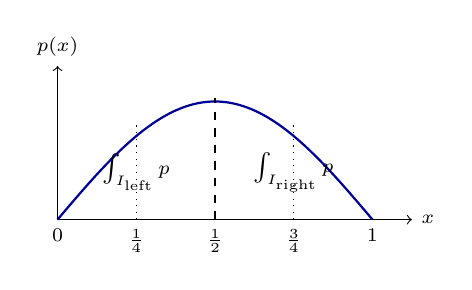
\begin{tikzpicture}[scale=1]
  \draw[->](0,0)--(4.5,0) node[right,font=\scriptsize]{$x$};
  \draw[->](0,0)--(0,1.95) node[above,font=\scriptsize]{$p(x)$};
  \draw[thick,blue!60!black,domain=0:1,smooth,variable=\x,samples=50]
       plot ({4*\x},{1.5*sin(180*\x)});
  \draw[dashed](2,0)--(2,1.55);
  \draw[dotted](1,0)--(1,1.25);  \draw[dotted](3,0)--(3,1.25);
  \foreach \px/\lab in {0/$0$,1/$\frac14$,2/$\frac12$,3/$\frac34$,4/$1$}
     \node[font=\scriptsize,below] at (\px,0){\lab};
  \node[font=\scriptsize] at (1,0.6){$\int_{I_{\mathrm{left}}}p$};
  \node[font=\scriptsize] at (3,0.6){$\int_{I_{\mathrm{right}}}p$};
\end{tikzpicture}
\caption{Grover--Rudolph 以二进分二分法分割质量。第一个比特的第一层旋转取
$\cos^2(\theta/2)=\int_{I_{\mathrm{left}}}p\big/\int_{[0,1)}p$（虚线分隔在 $\tfrac12$ 处）；随后每个
比特二分存留的区间（点线分隔在 $\tfrac14,\tfrac34$ 处），故第 $k$ 层携带 $2^{k-1}$ 个条件旋转。}
\label{fig:lec06-gr}
\end{figure}

关键在于\emph{为什么这只花 $\bigo(n)$ 个旋转}。在第 $k$ 层为 $2^{k-1}$ 个区间各硬编码一个单独的角度
会花掉 $\sum_{k=1}^{n}2^{k-1}=\bigo(2^{n})$——并不比一般的 \cref{prop:lec06-sp} 更好。增益完全
依赖于积分 $\int_{I}p$ 是\emph{经典可高效计算}这一假设：人们不去枚举区间，而是把已设定的比特
$i_1\cdots i_k$ 保存在一个寄存器中，由它们\emph{相干地}计算角度 $\theta$（在一个辅助比特上用 $p$ 的
累积分布做算术），作用一个由该寄存器所持角度决定的旋转，然后反计算。每一层都是一个这样的
$\poly(n)$ 门块，而共有 $n$ 层。一个告诫 (Herbert, 2021)：若积分只能由蒙特卡洛\emph{估计}而不能以
封闭形式求值，则采样代价可能抵消所加载态本应带来的那一份加速——因此该方法只对真正可积的密度
（对数凹、高斯及类似者）才有收益。
\end{remark}

\begin{example}[高效可积：四点上的 Grover--Rudolph]
\label{exa:lec06-grex}
在 $n=2$ 个量子比特上加载 $p=(3,1,1,3)/8$，即
$\ket{u}=\tfrac1{\sqrt8}\bigl(\sqrt3\,\ket{00}+\ket{01}+\ket{10}+\sqrt3\,\ket{11}\bigr)$。
以 $q_1$ 为最高有效位，两个半区 $\{00,01\}$ 与 $\{10,11\}$ 各携带相等的质量
$\tfrac12$，故第一层的角度满足 $\cos^2(\theta_1/2)=\tfrac12$，即对 $q_1$ 施加
$R_y(\pi/2)=\Hgate$。在 $q_1$ 的条件下，第二层的角度再把每一半区细分：
$q_1{=}0$ 给出 $\cos^2(\theta/2)=p_{00}/(p_{00}{+}p_{01})=\tfrac34$，故为 $R_y(\pi/3)$；
$q_1{=}1$ 给出 $p_{10}/(p_{10}{+}p_{11})=\tfrac14$，故为 $R_y(2\pi/3)$。于是第二层是一个
\emph{一致受控}（uniformly controlled）旋转——$q_1$ 的每个取值对应一个角度：
\begin{center}
\begin{quantikz}
  \lstick{$q_1:\ket0$} & \gate{\Hgate} & \octrl{1}          & \ctrl{1}            & \qw \\
  \lstick{$q_2:\ket0$} & \qw           & \gate{R_y(\pi/3)}  & \gate{R_y(2\pi/3)}  & \qw
\end{quantikz}
\end{center}
$\ket{00}$ 上的振幅为 $\cos\tfrac\pi4\cos\tfrac\pi6
=\tfrac1{\sqrt2}\cdot\tfrac{\sqrt3}2=\sqrt3/\sqrt8=\sqrt{p_{00}}$，正如所应。对于光滑的
密度，每一层的角度是在辅助比特上由 $\int_I p$ \emph{计算}得到、而非硬编码的，这正是
\cref{rem:lec06-gr} 的内容。
\end{example}

\begin{example}[稀疏向量]
\label{exa:lec06-sparsevec}
三量子比特态 $\ket{u}=\tfrac1{\sqrt2}(\ket{000}+\ket{101})$ 只有 $d=2$ 个非零振幅。
两个字上的相等权重由一个 Hadamard 和一个 $\CNOT$ 产生：对 $q_0$ 施加 $\Hgate$ 得到
$\tfrac1{\sqrt2}(\ket{000}+\ket{100})$，再用 $\CNOT_{q_0\to q_2}$ 翻转 $\ket{1\cdots}$
分支的最后一位，得到 $\ket{101}$。
\begin{center}
\begin{quantikz}
  \lstick{$q_0:\ket0$} & \gate{\Hgate} & \ctrl{2} & \qw \\
  \lstick{$q_1:\ket0$} & \qw           & \qw      & \qw \\
  \lstick{$q_2:\ket0$} & \qw           & \targ{}  & \qw
\end{quantikz}
\end{center}
一般而言，$d$-稀疏向量逐个振幅地加载：用 $\bigo(n)$ 个门寻址 $d$ 个位置中的每一个并
设定其大小与相位，共计 $\bigo(dn)$ 个门。
\end{example}

\begin{example}[矩阵乘积态：GHZ]
\label{exa:lec06-mps}
GHZ 态 $\ket{u}=\tfrac1{\sqrt2}(\ket{000}+\ket{111})$ 是最简单的非平凡矩阵乘积态，键维数
$\chi=2$。它的顺序式 MPS 制备就是教科书上的线路——对第一个量子比特施加 Hadamard，再接
一条沿寄存器传递键指标的 $\CNOT$ 链：
\begin{center}
\begin{quantikz}
  \lstick{$q_0:\ket0$} & \gate{\Hgate} & \ctrl{1} & \qw      & \qw \\
  \lstick{$q_1:\ket0$} & \qw           & \targ{}  & \ctrl{1} & \qw \\
  \lstick{$q_2:\ket0$} & \qw           & \qw      & \targ{}  & \qw
\end{quantikz}
\end{center}
每个门作用在 $\lceil\log_2\chi\rceil+1=2$ 个量子比特上，共有 $n-1$ 个，与
$\bigo(n\,\poly(\chi))$ 的计数相符；对更大的 $\chi$，这些 $\CNOT$ 换成 \cref{ch:lec15}
中的键酉算符。
\end{example}

\begin{remark}[一般 $n$ 的键维数：GHZ（$\chi=2$）与 Dicke（$\chi=3$）]
\label{rem:lec06-mpschi}
这两族都可推广到任意数目的量子比特，键指标恰好携带左块跨过某一割缝时必须传给右块的
那部分信息。

\emph{键维数 $2$（GHZ）。} $n$ 量子比特 GHZ 态
$\tfrac1{\sqrt2}(\ket0^{\otimes n}+\ket1^{\otimes n})$ 是具有对角 $2\times2$ 张量
$A^0=\proj0$、$A^1=\proj1$，以及边界余向量 $\bra{L}=\bra0+\bra1$、
$\ket{R}=\ket0+\ket1$ 的 MPS：乘积 $A^{x_1}\cdots A^{x_n}$ 仅当所有比特一致时才不为零
（任何混合串都含有一个因子 $\proj0\proj1=0$），只剩下两个均匀项。键只传递一个比特
——属于哪一支——故 $\chi=2$。顺序式线路为一个 $\Hgate$ 加上一条由 $n-1$ 个最近邻
$\CNOT$ 构成的链（此处以 $n=4$ 为例；那个被``携带''的单一量子比特\emph{就是}键）：
\begin{center}
\begin{quantikz}
  \lstick{$q_1:\ket0$} & \gate{\Hgate} & \ctrl{1} & \qw      & \qw      & \qw \\
  \lstick{$q_2:\ket0$} & \qw           & \targ{}  & \ctrl{1} & \qw      & \qw \\
  \lstick{$q_3:\ket0$} & \qw           & \qw      & \targ{}  & \ctrl{1} & \qw \\
  \lstick{$q_4:\ket0$} & \qw           & \qw      & \qw      & \targ{}  & \qw
\end{quantikz}
\end{center}

\emph{键维数 $3$（Dicke）。} 权重为 $2$ 的 Dicke 态
$\ket{D^n_2}=\binom n2^{-1/2}\sum_{\abs x=2}\ket x$ 是这样一个 MPS：其键指标
$m\in\{0,1,2\}$ 记录迄今已放置的 $1$ 的个数，张量为 $3\times3$ 的
\[
  A^0=\id_3,\qquad
  A^1=\begin{pmatrix}0&0&0\\ 1&0&0\\ 0&1&0\end{pmatrix},
\]
从起始键 $m=0$ 读到终止键 $m=2$。由于 $A^0$ 因子都是单位阵，乘积约化为
$(A^1)^{\abs x}$，而 $\bra{2}(A^1)^{\abs x}\ket0=\delta_{\abs x,2}$ 恰好挑出权重为 $2$ 的
串。跨过任一割缝，左块都必须宣告它已用掉多少个 $1$——$0$、$1$ 或 $2$，三条可区分的
消息——故施密特秩、也即键维数，为 $3$。（更一般地，$\ket{D^n_k}$ 有 $\chi=k+1$：键
一直计数到 $k$。）

\emph{代价。} 一个 $\chi$-MPS 由 $n$ 个顺序酉算符制备，每个作用在
$\lceil\log_2\chi\rceil+1$ 个量子比特上：GHZ（$\chi=2$，即上面的 $\Hgate$ 加 $\CNOT$
链）用两量子比特门，$\ket{D^n_2}$（$\chi=3$，一个 $\lceil\log_2 3\rceil=2$ 比特的键
寄存器依次与每个发射出的量子比特耦合）用三量子比特门——两种情形都是 $\bigo(n)$ 个门。
通用的单步复用键寄存器并发射一个物理量子比特：
\begin{center}
\begin{quantikz}
  \lstick{键 $\ket0$}   & \gate[3]{V_k} & \qw \\
  \lstick{键 $\ket0$}   &               & \qw \\
  \lstick{新鲜 $\ket0$} &               & \rstick{$q_k$}\qw
\end{quantikz}
\end{center}
依次施加 $V_1,\dots,V_n$ 并最终把键寄存器复位到 $\ket{00}$，便得到 $\ket{D^n_2}$；当
$\chi=2$ 时键是单个量子比特，每个 $V_k$ 即上面链中的那个两量子比特门。
\end{remark}

\begin{example}[显式的 Dicke 态 $\ket{D^3_2}$ 与 $\ket{D^4_2}$]
\label{exa:lec06-dicke34}
顺序式（MPS）制备背后的递推把第一个比特剥离出来：
\[
  \ket{D^n_k}=\sqrt{\tfrac{n-k}{n}}\,\ket0\otimes\ket{D^{n-1}_k}
             +\sqrt{\tfrac{k}{n}}\,\ket1\otimes\ket{D^{n-1}_{k-1}},
\]
因为在 $\binom nk$ 个权重为 $k$ 的串中，有 $(n-k)/n$ 的比例以 $0$ 开头、$k/n$ 的比例以 $1$ 开头。
将它展开即得显式的小线路。

\emph{$n=3$。} 以 $\ket{D^2_2}=\ket{11}$、$\ket{D^2_1}=\tfrac1{\sqrt2}(\ket{01}+\ket{10})$，
\[
  \ket{D^3_2}=\sqrt{\tfrac13}\,\ket0\ket{11}+\sqrt{\tfrac23}\,\ket1\ket{D^2_1}
             =\tfrac1{\sqrt3}\bigl(\ket{011}+\ket{101}+\ket{110}\bigr).
\]
分三步制备：对 $q_1$ 作 $R_y(\theta_1)$，$\theta_1=2\arccos\sqrt{\tfrac13}$（使
$q_1\mapsto\sqrt{\tfrac13}\ket0+\sqrt{\tfrac23}\ket1$）；在 $q_1{=}0$ 的条件下把 $q_2q_3$ 置为
$\ket{11}$；在 $q_1{=}1$ 的条件下在 $q_2q_3$ 上制备 $\ket{D^2_1}$（一个 $\Hgate$ 和一个 $\CNOT$，至多
差一次比特翻转）。由于对 $n=3$ 权重二是权重一的\emph{补}，等价地
$\ket{D^3_2}=X^{\otimes3}\ket{W_3}$，其中 $\ket{W_3}=\tfrac1{\sqrt3}(\ket{100}+\ket{010}+\ket{001})$。

\emph{$n=4$。} 此时 $\tfrac{n-k}{n}=\tfrac{k}{n}=\tfrac12$，故第一个旋转是 Hadamard：
\[
  \ket{D^4_2}=\tfrac1{\sqrt2}\,\ket0\ket{D^3_2}+\tfrac1{\sqrt2}\,\ket1\ket{W_3}
  =\tfrac1{\sqrt6}\bigl(\ket{0011}+\ket{0101}+\ket{0110}+\ket{1001}+\ket{1010}+\ket{1100}\bigr),
\]
这里用到 $\ket{D^3_1}=\ket{W_3}$。线路是：对 $q_1$ 作 $\Hgate$，再在 $q_1$ 控制下于 $q_2q_3q_4$ 上制备
——$q_1{=}0$ 时制备 $\ket{D^3_2}$，$q_1{=}1$ 时制备 $\ket{W_3}$——每个都是 $n=3$ 情形的三比特块。这就是
Bärtschi--Eidenbenz 递推；其扁平（非递归）版本复用单个``运行权重''辅助比特，达到
\cref{rem:lec06-mpschi} 所述的 $\bigo(kn)$ 门、$\bigo(n)$ 深度的线路。
\end{example}

\begin{example}[用相位梯度编码 $\sin(x_1+\cdots+x_d)$]
\label{exa:lec06-sinvec}
一个\emph{并非}各寄存器函数之乘积的函数，只要它的\emph{相位}是可乘的，仍可廉价地加载。
考虑 $d$ 个 $m$ 比特寄存器（每轴 $N=2^m$）上的实向量
$\ket\psi\propto\sum_{\mathbf x}\sin(x_1+\cdots+x_d)\,\ket{x_1}\cdots\ket{x_d}$。尽管
$\sin(\sum_k x_k)$ 不可因式分解，其相位却可以：
$\ee^{\ii\sum_k x_k}=\prod_{k}\prod_{b=0}^{m-1}\ee^{\ii 2^b(x_k)_b}$，于是\emph{相位梯度态}
\[
  \ket g=\sum_{\mathbf x}\ee^{\ii\sum_k x_k}\ket{\mathbf x}
   =\bigotimes_{k=1}^{d}\bigotimes_{b=0}^{m-1}\bigl(\ket0+\ee^{\ii 2^b}\ket1\bigr)
\]
是一个\emph{乘积}态——在 $dm$ 个量子比特的每一个上施加一个单比特相位
$P(2^b)=\diag(1,\ee^{\ii2^b})$（在一层 Hadamard 之后），没有任何纠缠门。\emph{相位梯度}
这一名称指的是相位在基上的分布方式：$\ket{\mathbf x}$ 的振幅携带相位 $\sum_k x_k$，它关于每个整数
坐标\emph{线性}增长——一个恒定的斜坡、即梯度——而比特 $b$ 贡献二进制加权的步长 $2^b$，这正是 QFT 与
Draper 加法器（\cref{sec:lec04-qftadder}）所用的那道相位阶梯。利用
$\sin\theta=(\ee^{\ii\theta}-\ee^{-\ii\theta})/2\ii$，
\[
  \ket\psi=\frac{1}{2\ii}\bigl(\ket g-\ket{g^{*}}\bigr),\qquad
  \ket{g^{*}}=\bigotimes_{k,b}\bigl(\ket0+\ee^{-\ii2^b}\ket1\bigr),
\]
这是一个两项组合，可用一个标志比特像 Hadamard 检验（\cref{sec:lec04-1}）那样提取：在数据上
制备均匀叠加、在标志上制备 $\ket+$，施加\emph{受标志控制}的相位梯度 $\Phi^{\pm}$（标志为
$\ket0$ 时相位取 $+2^b$，为 $\ket1$ 时取 $-2^b$），再对标志作 $\Hgate$ 并测量。
\begin{center}
\begin{quantikz}
  \lstick{$\ket0$ \,\scriptsize(标志)}  & \gate{\Hgate}              & \gate[2]{\Phi^{\pm}} & \gate{\Hgate} & \meter{} \\
  \lstick{$\ket{0^{dm}}$ \,\scriptsize(数据)} & \gate{\Hgate^{\otimes dm}} &                      & \qw           & \qw
\end{quantikz}
\end{center}
测得 $1$ 使数据处于归一化的正弦态
$\propto\sum_{\mathbf x}\sin(\sum_k x_k)\ket{\mathbf x}$；测得 $0$ 则给出\emph{余弦}态
$\propto\sum_{\mathbf x}\cos(\sum_k x_k)\ket{\mathbf x}$，即错误的向量——只需丢弃它并重跑这个（廉价的）
线路。标志读到 $1$ 的概率为 $N^{-d}\sum_{\mathbf x}\sin^2(\sum_k x_k)\approx\tfrac12$，故期望的尝试次数
为 $\bigo(1)$（约两次）；等价地，对标志作一轮振幅放大（\cref{ch:lec03}）即可使该制备\emph{确定化}、
无需重复。总代价是 $\bigo(dm)$ 个单比特与受控相位门——无需振幅加载、无需算术。同样的手法可编码任何线性型
$\sum_k a_k x_k$ 的 $\sin$ 或 $\cos$（相位取 $\ee^{\pm\ii a_k2^b}$）；只有取虚部这一步需要标志，
因为乘积 $\prod_k f_k(x_k)$ 本就可分解为单寄存器的制备。
\end{example}

\begin{remark}[可分离与相位多项式的变体]
\label{rem:lec06-phasepoly}
同样的想法按指数如何嵌入量子比特对相关编码作出分类。
\begin{itemize}[leftmargin=1.4em,nosep]
  \item \emph{可分离（最易）：$\ee^{\sum_k a_k x_k}$。}线性型的实指数\emph{可因式分解}，
        $\ee^{\sum_k a_k x_k}=\prod_{k,b}\ee^{a_k 2^b (x_k)_b}$，于是
        $\sum_{\mathbf x}\ee^{\sum_k a_k x_k}\ket{\mathbf x}
        =\bigotimes_{k,b}\bigl(\ket0+\ee^{a_k 2^b}\ket1\bigr)$ 是一个\emph{乘积}态——每个
        量子比特上一个单比特旋转 $R_y(\theta_{k,b})$，其中 $\theta_{k,b}$ 使寄存器 $k$ 的第 $b$ 个
        比特倾斜为 $R_y(\theta_{k,b})\ket0\propto\ket0+\ee^{a_k 2^b}\ket1$，即
        $\tan(\theta_{k,b}/2)=\ee^{a_k 2^b}$，等价地 $\theta_{k,b}=2\arctan(\ee^{a_k 2^b})$；
        既无辅助比特也无纠缠门。（各振幅跨越双指数的量级，故通常对自变量重标度，如 $\ee^{-a_k x_k}$，以免
        态坍缩到单一角点。）
  \item \emph{相位多项式：$\sin(x_1x_2\cdots x_d)$。}此时指数是一个\emph{乘积}。按比特展开，
        $x_1\cdots x_d=\sum_{b_1,\dots,b_d}2^{b_1+\cdots+b_d}(x_1)_{b_1}\cdots(x_d)_{b_d}$，
        故 $\ee^{\ii x_1\cdots x_d}$ 是 $m^d$ 个多重受控相位
        $C^{d-1}P\bigl(2^{\sum_k b_k}\bigr)$ 之积（仅当 $d$ 个被选比特全为 $1$ 时才施加相位）。
        于是 $\ket g=\sum_{\mathbf x}\ee^{\ii x_1\cdots x_d}\ket{\mathbf x}$ 是
        $\Hgate^{\otimes dm}$ 后接那 $m^d$ 个受控相位——有纠缠，但对固定 $d$ 为 $\poly(m)$——而
        $\sin(x_1\cdots x_d)$ 是其虚部，用 \cref{exa:lec06-sinvec} 的单标志步骤读出。代价关于
        $d$ 是指数的（$d$ 次单项式的个数），这是真正多线性指数的代价。
\end{itemize}
一般地，若 $f(\mathbf x)=\ee^{\ii\varphi(\mathbf x)}$ 的实部或虚部、而 $\varphi$ 是一个多线性
相位多项式，则相位态是一层（多重）受控相位——每个单项式一个——而单个标志比特把复相位态
转为实的 $\sin/\cos$ 振幅向量。
\end{remark}

\begin{example}[径向振幅 $1/\lvert\mathbf x\rvert$ 作为高斯之和]
\label{exa:lec06-coulomb}
库仑型向量 $1/\lvert\mathbf x\rvert$（$\lvert\mathbf x\rvert=\sqrt{x_1^2+\cdots+x_d^2}$）
既不可分离、也非相位多项式——和的平方根同时挫败了这两种技巧。标准手段是一个恢复可分离性的
\emph{积分表示}：
\[
  \frac{1}{\lvert\mathbf x\rvert}
  =\frac{2}{\sqrt\pi}\int_0^\infty \ee^{-\lvert\mathbf x\rvert^2 t^2}\,dt
  =\frac{2}{\sqrt\pi}\int_0^\infty \prod_{k=1}^d \ee^{-x_k^2 t^2}\,dt
  \qquad(\mathbf x\neq0),
\]
其被积函数是一个\emph{可分离}的高斯函数。把 $t$ 离散化到几何网格 $\{t_q\}$ 并配以权重
$\{w_q\}$（高斯型求积，$Q=\bigo\bigl(\log\tfrac1\epsilon\,\log\tfrac{r_{\max}}{r_{\min}}\bigr)$
个节点即足够，Beylkin--Monzón），便化为乘积态的有限线性组合，
\[
  \sum_{\mathbf x}\frac{1}{\lvert\mathbf x\rvert}\ket{\mathbf x}
  \ \approx\ \sum_{q} w_q\,\bigotimes_{k=1}^{d}
     \Bigl(\sum_{x_k}\ee^{-x_k^2 t_q^2}\ket{x_k}\Bigr).
\]
这里 $\mathbf x=(x_1,\dots,x_d)$ 是一个格点的 $d$ 个空间\emph{坐标}——$d$ 个数据寄存器的内容，即我们
所叠加的变量——而 $t_q$ 是\emph{求积节点}（高斯的宽度），一张预先固定的、含 $Q$ 个数的经典列表；二者
不应混淆。每个一维高斯寄存器 $\sum_{x_k}\ee^{-x_k^2 t_q^2}\ket{x_k}$ 是一个\emph{高效可积}分布，由
Grover--Rudolph（\cref{exa:lec06-grex}）用 $\bigo(m)$ 个受控旋转制备；这 $Q$ 项则由
\cref{ch:lec07} 的向量加法（LCU）基本操作组合起来——一个 $\lceil\log_2 Q\rceil$ 比特的索引
寄存器由 $\mathrm{PREP}$ 加载 $\sqrt{w_q}$，一个 $\mathrm{SEL}$ 受索引控制地制备宽度为 $t_q$
的高斯乘积，最后对索引标志作后选择：
\begin{center}
\begin{quantikz}
  \lstick{$\ket{0^{\lceil\log Q\rceil}}$ \,\scriptsize(索引)} & \gate{\mathrm{PREP}} & \ctrl{1} & \gate{\mathrm{PREP}^{\dagger}} & \meter{} \\
  \lstick{$\ket{0^{dm}}$ \,\scriptsize(数据 $x_1,\dots,x_d$)}  & \qwbundle{dm}        & \gate{\mathrm{SEL}} & \qw                    & \qw
\end{quantikz}
\end{center}
其中 $\mathrm{SEL}=\sum_q\proj{q}\otimes O_q$，而 $O_q$ 制备
$\bigotimes_k(\sum_{x_k}\ee^{-x_k^2 t_q^2}\ket{x_k})$。总代价为 $\bigo(Qdm)$ 个门，索引标志被
测得的概率为
$\lVert\sum_{\mathbf x}\lvert\mathbf x\rvert^{-1}\ket{\mathbf x}\rVert^2/\lVert w\rVert_1^2$。
同样的高斯求和配方可编码任何具有已知一维变换的径向函数——$\lvert\mathbf x\rvert^{-s}$、
$\ee^{-\mu\lvert\mathbf x\rvert}$、汤川核 $\ee^{-\mu\lvert\mathbf x\rvert}/\lvert\mathbf x\rvert$——
并支撑着库仑相互作用的量子处理。
\end{example}

\begin{remark}[用算术加载实多项式振幅：$\sum_{i\neq j}x_ix_j$]
\label{rem:lec06-polyamp}
当目标振幅是一个\emph{实多项式}、而非某个相位的实部或虚部时，相位梯度技巧不再直接适用；
通用工具是\emph{计算–旋转–反计算}。取 $f(\mathbf x)=\sum_{i\neq j}x_ix_j$。先作代数化简，
\[
  \sum_{i\neq j}x_ix_j=\Bigl(\sum_i x_i\Bigr)^{\!2}-\sum_i x_i^{2}=S^2-Q,
\]
于是 $f$ 只需线性型 $S=\sum_i x_i$（一棵 $\bigo(\log d)$ 深的模加法器之树，
\cref{sec:lec04-qftadder}）以及可分离的平方和 $Q=\sum_i x_i^2$（对每个寄存器平方后相加）。
用可逆算术把 $f(\mathbf x)=S^2-Q$ 算入一个工作寄存器，再按寄存器所存之值施加旋转
$R_y\!\bigl(2\arcsin(f(\mathbf x)/F)\bigr)$（$F=\max_{\mathbf x}\abs{f(\mathbf x)}$）到一个
信号比特上，最后反计算工作寄存器：
\begin{center}
\begin{quantikz}
  \lstick{$\ket{\mathbf x}$ \,\scriptsize(数据)}   & \gate[2]{\textsc{arith}} & \qw          & \gate[2]{\textsc{arith}^{\dagger}} & \qw \\
  \lstick{$\ket{0}$ \,\scriptsize(工作)}           &                          & \gate[2]{R_y} &                                   & \qw \\
  \lstick{$\ket{0}$ \,\scriptsize(信号)}           & \qw                      &               & \qw                               & \qw
\end{quantikz}
\end{center}
这正是用可逆数据通路实现的 \eqref{eq:lec06-OA} 之条目谕示 $O_A$。方框 $\textsc{arith}$ 就是这条数据
通路：它读入数据寄存器 $\ket{\mathbf x}$，用普通的可逆整数算术把 $f(\mathbf x)$ 写入一个新鲜的工作
寄存器——一棵计算 $S=\sum_i x_i$ 的加法器树、对每个 $x_i^2$（以及 $S^2$）的平方电路、以及形成 $S^2-Q$
的减法器——使得 $\textsc{arith}\,\ket{\mathbf x}\ket0=\ket{\mathbf x}\ket{f(\mathbf x)}$。旋转 $R_y$
\emph{受工作寄存器所存之值控制}（一个按寄存器编码之角度的旋转，如 \cref{rem:lec06-gr}），而
$\textsc{arith}^{\dagger}$ 把同一数据通路反向运行，把工作寄存器清回 $\ket0$，不留下与数据纠缠的垃圾。
净效果使信号携带振幅 $f(\mathbf x)/F$，故在均匀数据态上对信号作后选择即得
$\propto\sum_{\mathbf x}f(\mathbf x)\ket{\mathbf x}$，用 $\poly(d,m)$ 个门。同一配方可加载任何高效可
计算的实振幅（唯一改变的是 $\textsc{arith}$）。

还有一种避开算术但为近似的相位态方案：由于每个 $x_ix_j$ 是双线性的，
$\ee^{\ii\theta f(\mathbf x)}=\prod_{i\neq j}\prod_{a,b}
\ee^{\ii\theta 2^{a+b}(x_i)_a(x_j)_b}$ 是 $\bigo(d^2m^2)$ 个受控相位门之积（\cref{rem:lec06-phasepoly}
的两寄存器推广）；对小的 $\theta$，\cref{exa:lec06-sinvec} 的正弦态给出
$\sum_{\mathbf x}\sin(\theta f)\ket{\mathbf x}\approx\theta\sum_{\mathbf x}f\,
\ket{\mathbf x}$，即目标态，误差为 $\bigo(\theta^2)$、重复开销为 $\bigo(1/\theta^2)$。
\end{remark}

\begin{remark}[易于制备的振幅向量工具箱]
\label{rem:lec06-toolbox}
上面的例子都是少数几种\emph{结构性抓手}的实例，每一种都击败了 \cref{prop:lec06-sp} 的一般
$\Omega(2^n/n)$ 下界。只要 $f$ 具有以下形式之一，向量
$\sum_{\mathbf x}f(\mathbf x)\ket{\mathbf x}$ 便可高效制备。
\begin{itemize}[leftmargin=1.4em,nosep]
  \item \emph{可分离}，$f(\mathbf x)=\prod_k f_k(x_k)$：单寄存器制备的张量积——$\bigo(dm)$ 个门、
        无纠缠（\cref{exa:lec06-prod}；\cref{rem:lec06-phasepoly} 中的 $\ee^{\sum a_kx_k}$）。
  \item \emph{有界键维数}，即跨每条割缝的施密特秩 $\le\chi$：一个矩阵乘积态，顺序制备，
        $\bigo(n\,\poly\chi)$ 个门（\cref{exa:lec06-mps,rem:lec06-mpschi}——GHZ、$W$、Dicke）。
  \item \emph{高效可积的密度}，$f=\sqrt{p}$ 且累积分布可经典计算：Grover--Rudolph，用
        $\bigo(n)$ 个受控旋转（\cref{exa:lec06-grex}——高斯、对数凹分布）。
  \item \emph{低次多项式的相位}，$f=\ee^{\ii\varphi}$ 的实部或虚部：一层（多重）受控相位，
        每个单项式一个，外加一个取实/虚部的标志比特（\cref{exa:lec06-sinvec,rem:lec06-phasepoly}）。
  \item \emph{在易算函数上的短展开}，$f=\sum_{k} c_k b_k$，其中每个 $b_k$ 是相位梯度（傅里叶
        模）、高斯或单项式：用 \cref{ch:lec07} 的线性组合（向量加法）基本操作把各项合并。这涵盖
        截断的傅里叶／切比雪夫级数以及径向积分变换核 $1/\lvert\mathbf x\rvert$、
        $\ee^{-\mu\lvert\mathbf x\rvert}$（\cref{exa:lec06-coulomb}）。
  \item \emph{任何高效可计算的振幅}：用一个 $\poly$ 规模的可逆线路算出 $f(\mathbf x)$，按寄存器
        所存之值旋转一个信号比特，再反计算——即以数据通路实现的条目谕示 $O_A$
        （\cref{rem:lec06-polyamp}）。只要已知 $f$ 的公式，这便是通用的退路。
  \item \emph{稀疏}，仅有 $d=\poly(n)$ 个非零元：逐个加载，$\bigo(dn)$ 个门
        （\cref{exa:lec06-sparsevec}）；若以上皆不适用，QRAM 以 $\bigo(2^n)$ 的硬件代价在
        $\bigo(n)$ 深度内给出任意向量。
\end{itemize}
这些抓手可以\emph{复合}：易因子之积、易项之 LCU、易公式之振幅加载，仍然是易的；因此实践中遇到
的大多数结构化向量——光滑密度、低秩态、局域哈密顿量基态拟设、离散化的光滑函数——都落入这些类
之一或其组合。一个\emph{毫无}这些结构的向量（一般单位向量、密码学或伪随机的振幅分布）才是真正
昂贵的，达到 \cref{prop:lec06-sp} 的界。
\end{remark}

此后我们将 $O_u$ 视为一个给定的谕示，并计数对它的\emph{查询}，正如我们在 \cref{ch:lec05} 中计数对
$\ee^{-\ii Ht}$ 的查询那样。态制备谕示是输入模型的向量那一半；本讲余下部分构建矩阵那一半。
\section{块编码：定义与因子}
\label{sec:lec06-2}

非酉的 $A$ 无法由线路直接实现。块编码 (block encoding) 的思想是把 $A$ 的一个缩放副本
放进一个更大酉算符的某个\emph{块}中，并通过借助辅助比特 (ancilla) 投影到该块上来访问它。

\subsection*{单辅助比特图景}

从最简单的情形开始。假设我们能找到一个 $(n+1)$ 比特酉算符 $U_A$，其左上角的 $n$ 比特块等于 $A$，
\begin{equation}
  U_A=\begin{pmatrix} A & \ast\\ \ast & \ast\end{pmatrix},
  \label{eq:lec06-block1}
\end{equation}
其中 $\ast$ 表示与计算无关的块。对任意 $n$ 比特态
$\ket{b}$，输入带标志的态 $\ket{0}\ket{b}$：
\begin{equation}
  U_A\ket{0}\ket{b}=\ket{0}\,A\ket{b}+\ket{1}\ket{\perp},
  \label{eq:lec06-apply1}
\end{equation}
其中 $\ket{\perp}$ 是某个（未归一化的）态。要理解这一点，把每个 $(n+1)$ 比特
向量按其辅助比特分成一个\emph{顶}块（辅助比特 $\ket0$）和一个
\emph{底}块（辅助比特 $\ket1$），二者各为一个 $n$ 比特向量。（我们把辅助比特置于\emph{前导}寄存器，
故 $\ket0\ket b=\ket0\otimes\ket b
=\left(\begin{smallmatrix}\ket b\\ 0\end{smallmatrix}\right)$，而
$\ket1\ket b=\left(\begin{smallmatrix}0\\ \ket b\end{smallmatrix}\right)$：辅助比特
的 $\ket0$ 与 $\ket1$ 振幅选择顶块与底块。）在
此划分下，带标志的输入其底块为零，
$\ket{0}\ket{b}=\left(\begin{smallmatrix}\ket b\\ 0\end{smallmatrix}\right)$，于是，
把 $U_A$ 的左下块记为 $C$，
\[
  U_A\ket{0}\ket{b}
   =\begin{pmatrix}A&\ast\\ C&\ast\end{pmatrix}\!
    \begin{pmatrix}\ket b\\ 0\end{pmatrix}
   =\begin{pmatrix}A\ket b\\ C\ket b\end{pmatrix}
   =\ket{0}\,A\ket{b}+\ket{1}\,\ket{\perp},
   \qquad \ket{\perp}\defeq C\ket{b}.
\]
由于输入的底块为零，只有 $U_A$ 的第一\emph{块列}被探测；在该列中顶块 $A$ 产生辅助比特为 $\ket0$ 的部分
$\ket0\,A\ket b$，而左下块 $C$ 则把剩余振幅倾倒进
辅助比特为 $\ket1$ 的``垃圾''态 $\ket{\perp}$（未归一化，且一旦我们
进行后选择便无关紧要）。等价地，
$(\bra{0}\otimes\id)\,U_A\,(\ket{0}\otimes\id)=A$：把 $U_A$ 夹在
辅助比特标志 $\ket0$ 之间恰好抽取其左上块。测量辅助比特并保留
结果 $0$，系统便留在归一化态 $A\ket{b}/\norm{A\ket{b}}$ 上，
其以成功概率
\begin{equation}
  p(0)=\norm{A\ket{b}}^2=\bra{b}A\dg A\ket{b}.
  \label{eq:lec06-prob1}
\end{equation}
获得。于是那个``缺失''的标量 $\norm{A\ket{b}}$ 可从测量
统计中恢复；它只依赖于 $A$ 与 $\ket{b}$，而不依赖于 $U_A$ 的无关块。由于酉算符的一个块的算符范数至多为 $1$，
嵌入 \eqref{eq:lec06-block1} 要求 $\norm{A}\le1$。

\subsection*{缩放与一般定义}

大多数感兴趣的矩阵满足 $\norm{A}>1$，或者根本无法将 $A$ 精确嵌入。
通过允许 $U_A$ 编码 $A/\alpha$（其中 $\alpha\ge\norm{A}$ 为一个
\emph{子归一化因子} (subnormalization factor)）、使用 $a$ 个辅助比特，并
容忍误差 $\epsilon$，这两个障碍都可被消除。

\begin{definition}[块编码]
\label{def:lec06-be}
设 $A$ 为一个 $n$ 比特矩阵，并设 $\alpha,\epsilon\ge0$ 且 $a\in\N$。一个
$(a+n)$ 比特酉算符 $U_A$ 称为 $A$ 的 \emph{$(\alpha,a,\epsilon)$-块编码}，
如果
\begin{equation}
  \norm{\,A-\alpha\,\bigl(\bra{0^a}\otimes\id_n\bigr)\,U_A\,
         \bigl(\ket{0^a}\otimes\id_n\bigr)\,}\le\epsilon.
  \label{eq:lec06-bedef}
\end{equation}
当 $\epsilon=0$ 时该编码是\emph{精确的}，$U_A$ 称为
$(\alpha,a)$-块编码。我们记 $U_A\in\mathrm{BE}_{\alpha,a}(A,\epsilon)$，
以及 $\mathrm{BE}_{\alpha,a}(A)=\mathrm{BE}_{\alpha,a}(A,0)$。
\end{definition}

等价地，在精确情形下，$U_A$ 的左上角 $n$ 比特块等于
$A/\alpha$：
\begin{equation}
  \bigl(\bra{0^a}\otimes\id_n\bigr)\,U_A\,\bigl(\ket{0^a}\otimes\id_n\bigr)
  =\frac{A}{\alpha},
  \qquad
  U_A=\begin{pmatrix} A/\alpha & \ast\\ \ast & \ast\end{pmatrix},
  \label{eq:lec06-bealt}
\end{equation}
其具有 $2^{a}$ 个块行与块列。这三个参数是第~II~部分的通货：
\begin{itemize}[leftmargin=1.4em,nosep]
  \item $\alpha$（\emph{子归一化因子}）把 $A$ 缩放进一个
        酉算符的块中，因而遵从 $\alpha\ge\norm{A}$。它并非免费：将 $U_A$ 作用于
        $\ket{0^a}\ket{b}$ 产生 $\ket{0^a}(A/\alpha)\ket{b}+\ket{\perp}$，故
        标志 $\ket{0^a}$ 以概率
        $\norm{A\ket{b}}^2/\alpha^2$ 被读出。更大的 $\alpha$ 缩小成功
        概率，更重要的是，将每一个下游算法（QSVT、QLSP）的查询代价
        乘以 $\alpha$。因此让 $\alpha$ 接近
        $\norm{A}$ 是一个核心的设计目标。
  \item $a$ 是辅助（标志）比特的数目；有用的子空间由
        $\ket{0^a}$ 标志。
  \item $\epsilon$ 是谱范数误差，它通过 \cref{ch:lec07} 的算术以加法方式传播。
\end{itemize}

验证规则值得单独陈述，因为它被不断用到。

\begin{remark}[逐元验证块编码]
\label{rem:lec06-verify}
$U_A\in\mathrm{BE}_{1,a}(A)$ 当且仅当对所有 $i,j\in[N]$ 有
$\bra{0^a,i}U_A\ket{0^a,j}=A_{ij}$，其中
$\ket{0^a,j}\defeq\ket{0^a}\ket{j}$。当 $U_A=U_BU_C$ 分解时，可通过拆分乘积来计算
矩阵元，
$\bra{0^a,i}U_A\ket{0^a,j}=\bigl(U_B\dg\ket{0^a,i}\bigr)\dg\bigl(U_C\ket{0^a,j}\bigr)$，
分别独立地求出这两个态并取其内积。这是下面每一个构造的
主力计算。
\end{remark}

\subsection*{每个压缩映射都可块编码}

块编码在原理上并非一个限制性假设——它正是任何
压缩映射 (contraction) 被访问的方式——如下面的构造所示。

\begin{proposition}[$(1,1)$-块编码对压缩映射是通用的]
\label{prop:lec06-svd}
每个满足 $\norm{A}\le1$ 的 $n$ 比特矩阵 $A$ 都容许一个精确的
$(1,1)$-块编码。
\end{proposition}

\begin{proof}
设 $A=W\Sigma V\dg$ 为一个奇异值分解 (SVD)，其中 $W,V$ 酉，且
$\Sigma=\diag(\sigma_1,\dots,\sigma_N)$，由于 $\norm{A}\le1$ 故 $\sigma_i\in[0,1]$。
因为 $\sigma_i\le1$，对角矩阵 $\sqrt{\id-\Sigma^2}$ 为实，而
$(n+1)$ 比特矩阵
\begin{equation}
  U_A=\begin{pmatrix} W & 0\\ 0 & \id_n\end{pmatrix}
      \begin{pmatrix} \Sigma & \sqrt{\id_n-\Sigma^2}\\
                      \sqrt{\id_n-\Sigma^2} & -\Sigma\end{pmatrix}
      \begin{pmatrix} V\dg & 0\\ 0 & \id_n\end{pmatrix}
  \label{eq:lec06-svd}
\end{equation}
是酉的：外侧因子是酉的，而中间因子是酉的，因为
每个 $2\times2$ 块 $\left(\begin{smallmatrix}\sigma_i&\sqrt{1-\sigma_i^2}\\
\sqrt{1-\sigma_i^2}&-\sigma_i\end{smallmatrix}\right)$ 是一个反射（其各列
标准正交）。其左上块为 $W\Sigma V\dg=A$，所以
$U_A\in\mathrm{BE}_{1,1}(A)$。
\end{proof}

\cref{prop:lec06-svd} 表明块编码在原理上不花任何代价。第~II~部分的内容
在于：对于\emph{结构化}的 $A$——稀疏矩阵（\cref{sec:lec06-3}）、
块编码的和与积（\cref{ch:lec07}）、以及源自
物理哈密顿量的矩阵——人们可以用一个 $\polylog(N)$ 规模的线路和一个
小因子 $\alpha$ 构造出 $U_A$，使得整条流水线保持高效。

\begin{example}[对一个 $2\times2$ 矩阵做块编码；读出 $\alpha$]
\label{exa:lec06-2x2}
考虑单量子比特矩阵
\[
  A=\begin{pmatrix} 1 & 1\\ 0 & 1\end{pmatrix}.
\]
其奇异值 $\sigma_\pm$ 满足 $\sigma_+\sigma_-=\abs{\det A}=1$ 且
$\sigma_+^2+\sigma_-^2=\tr(A^\top A)=3$，故 $\sigma_\pm^2=(3\pm\sqrt5)/2$，即
$\sigma_\pm=\varphi^{\pm1}$，其中 $\varphi=\tfrac{1+\sqrt5}{2}\approx1.618$ 为黄金比例
(golden ratio)；于是 $\norm{A}=\sigma_+=\varphi$。由于 $\norm{A}>1$，不存在精确的
$(1,\cdot)$-块编码；取 $\alpha=2\ge\norm{A}$，并令
\[
  M\defeq\frac{A}{\alpha}=\begin{pmatrix}1/2&1/2\\0&1/2\end{pmatrix},
  \qquad \norm{M}=\frac{\varphi}{2}\approx0.809<1 ,
\]
它是一个压缩映射 (contraction)。\cref{prop:lec06-svd} 的膨胀 (dilation) 通过添加亏损块
(defect block) $\sqrt{\id-MM^\top}$ 与 $\sqrt{\id-M^\top M}$ 把 $M$ 补全为一个酉算符：
\[
  U_A=\begin{pmatrix} M & \sqrt{\id-MM^\top}\\[3pt]
                      \sqrt{\id-M^\top M} & -M^\top\end{pmatrix}
     \approx\begin{pmatrix}
        0.5 & 0.5 & 0.688 & -0.162\\
        0   & 0.5 & -0.162 & 0.851\\
        0.851 & -0.162 & -0.5 & 0\\
        -0.162 & 0.688 & -0.5 & -0.5
      \end{pmatrix},
\]
这是一个货真价实的 $2$ 比特正交矩阵（一个标志比特与一个系统比特），其左上角的
$2\times2$ 块恰为 $M=A/\alpha$；这便是 $A$ 的一个 $(2,1)$-块编码。两个亏损块正是上面
示意形式中带星的元，它们（在膨胀的符号约定下）由要求各列标准正交所确定。

将 $U_A$ 作用于 $\ket{0}\ket{b}$ 并在标志 $\ket{0}$ 上进行后选择，便以概率
$\norm{A\ket{b}}^2/\alpha^2$ 返回 $A\ket{b}/\norm{A\ket{b}}$。具体地，对
$\ket{b}=\ket{0}$ 有 $A\ket{0}=\ket{0}$，故 $\norm{A\ket{0}}^2=1$，成功概率为
$1/\alpha^2=1/4$；对 $\ket{b}=\ket{1}$ 有 $A\ket{1}=\ket{0}+\ket{1}$，故
$\norm{A\ket{1}}^2=2$，概率为 $2/4=1/2$。倘若我们浪费地选取 $\alpha=10$，同样的输出
态仍会出现，但这两个概率会降到 $1/100$ 与 $1/50$——小了 $(\alpha/2)^2=25$ 倍，直接拉长
了运行时间。这正是``让 $\alpha$ 接近 $\norm{A}$''的实践含义。
\end{example}
\section{矩阵–向量乘法 (matrix--vector multiplication)：第一个基本操作}
\label{sec:lec06-matvec}

有了这两种输入模型，我们已经可以执行最基本的
量子数值线性代数运算：给定作为块编码 (block encoding) 的矩阵 $A$
和作为态制备谕示 (state-preparation oracle) 的向量 $b$，产生归一化的
矩阵–向量乘积 $A\ket{b}/\norm{A\ket{b}}$。这一个基本操作正是
线性求解器、幂迭代以及对模拟态
$\ee^{-\ii Ht}\ket{b}$ 的读出背后的引擎。

\begin{proposition}[将块编码作用于一个态]
\label{prop:lec06-matvec}
设 $U_A\in\mathrm{BE}_{\alpha,a}(A)$，并设 $O_b$ 制备出 $\ket{b}=O_b\ket{0^n}$。
则
\[
  U_A\,\bigl(\id_a\otimes O_b\bigr)\ket{0^a}\ket{0^n}
  =\ket{0^a}\,\frac{A\ket{b}}{\alpha}+\ket{\Phi^{\perp}},
  \qquad \bigl(\proj{0^a}\otimes\id\bigr)\ket{\Phi^{\perp}}=0,
\]
且对 $a$ 量子比特标志位进行测量以概率
$p=\norm{A\ket{b}}^2/\alpha^2$ 返回 $\ket{0^a}$，此时系统寄存器坍缩到
$A\ket{b}/\norm{A\ket{b}}$。
\end{proposition}

\begin{proof}
$O_b$ 产生 $\ket{0^a}\ket{b}$；作用 $U_A$ 并利用
$(\bra{0^a}\otimes\id)U_A(\ket{0^a}\otimes\id)=A/\alpha$（\cref{def:lec06-be}）即得
所述的分解，其标志位为 $\ket{0^a}$ 的部分是 $\ket{0^a}(A/\alpha)\ket{b}$。它的
模方 $\norm{(A/\alpha)\ket{b}}^2=\norm{A\ket{b}}^2/\alpha^2$ 即为
读到 $\ket{0^a}$ 的概率，而测量后的系统态是
归一化的 $A\ket{b}/\norm{A\ket{b}}$。
\end{proof}

有三个特征使它成为第二部分所有内容的模板。
\begin{itemize}[leftmargin=1.4em,nosep]
  \item \emph{输入与输出共享同一种格式。} 结果仍是一个 $n$ 量子比特
        态，与输入 $\ket{b}$ 一样。因此块编码既是一种\emph{输入}
        模型也是一种\emph{输出}模型：乘积可直接馈入另一个块
        编码，于是矩阵–向量乘积链式串接为 $A_k\cdots A_1\ket{b}$，无需
        读出中间向量。
  \item \emph{代价由 $\alpha$ 和输出范数决定。} 单次运行以
        概率 $p=\norm{A\ket{b}}^2/\alpha^2$ 成功，故朴素重复的代价为
        $\bigo(\alpha^2/\norm{A\ket{b}}^2)$ 次查询。振幅放大
        （\cref{thm:lec03-aa}）去掉了平方，将其降为
        对 $U_A$ 和 $O_b$ 的 $\bigo\!\bigl(\alpha/\norm{A\ket{b}}\bigr)$ 次查询——即
        使该基本操作值得采用的平方增益，也是把 $\alpha$ 保持得小的
        定量理由：每一次矩阵–向量乘积都要为它线性地付出代价。
  \item \emph{只产生方向。} 标量 $\norm{A\ket{b}}$ 不由
        输出态携带；它从成功概率中恢复为
        $\norm{A\ket{b}}=\alpha\sqrt p$，正如一个被制备向量的范数在
        \cref{sec:lec06-1} 中必须在经典一侧被追踪那样。
\end{itemize}

\begin{example}[用 $2\times2$ 编码做矩阵–向量乘积]
\label{exa:lec06-matvec}
取 $A=\left(\begin{smallmatrix}1&1\\0&1\end{smallmatrix}\right)$，并用
\cref{exa:lec06-2x2} 的 $(2,1)$-块编码（$\alpha=2$）。对于 $\ket{b}=\ket{0}$
（故 $O_b=\id$），$A\ket{0}=\ket{0}$，$\norm{A\ket{0}}=1$，因此标志位以
概率 $p=1/\alpha^2=1/4$ 被读到，输出为 $\ket{0}$。对于 $\ket{b}=\ket{1}$，
$A\ket{1}=\ket{0}+\ket{1}$ 有 $\norm{A\ket{1}}=\sqrt2$，给出 $p=2/4=1/2$ 和输出
$(\ket{0}+\ket{1})/\sqrt2$。输出范数越大，成功概率
越大；倘若我们采用 \cref{exa:lec06-2x2} 中浪费的 $\alpha=10$，两个
概率都会下降 $25$ 倍。
\end{example}

块编码与态制备谕示也可以\emph{组合}出新的编码：人们可以把两个块编码的矩阵相加、把
两个制备好的向量相加，以及把两个块编码的矩阵相乘，使得输出再次是一个块编码（或一个
态），可供下一步使用。每一条这样的规则都是\emph{酉算符线性组合} (linear combination
of unitaries, LCU) 的特例，因此我们把它们放在一起处理——面向任意多个项，连同其线路、
误差传播与 $\ell^1$ 范数代价——详见 \cref{ch:lec07}。

\section{\texorpdfstring{$s$}{s}-稀疏矩阵的块编码}
\label{sec:lec06-3}

我们现在给出标准的高效构造：由两个谕示（oracle）构建的稀疏矩阵块编码（block encoding）——一个提供条目\emph{值}，一个提供非零\emph{位置}。几乎所有 QNLA 复杂度都是在这一模型下陈述的。

\subsection*{条目谕示与位置谕示}

假设 $\norm{A}_{\max}\defeq\max_{ij}\abs{A_{ij}}\le1$（否则将 $A$ 按
$\norm{A}_{\max}$ 重新标度）。\emph{条目谕示}（entry oracle）通过一个受控旋转把每个矩阵元编码到一个信号量子比特的振幅中：
\begin{equation}
  O_A\ket{0}\ket{i}\ket{j}
   =\Bigl(A_{ij}\ket{0}+\sqrt{1-\abs{A_{ij}}^2}\,\ket{1}\Bigr)\ket{i}\ket{j}.
  \label{eq:lec06-OA}
\end{equation}
（在实践中，一个返回 $A_{ij}$ 的 $d$ 比特表示的数据库谕示
$\widetilde O_A\ket{0^{d}}\ket{i}\ket{j}=\ket{\tilde A_{ij}}\ket{i}\ket{j}$ 通过一个受控旋转、再对工作寄存器反计算，即可转化为 \eqref{eq:lec06-OA}。）若一个矩阵的每一行和每一列至多有 $s$ 个非零条目，则称它是 \emph{$s$-稀疏}（$s$-sparse）的；\emph{位置谕示}（location oracle）将这些非零条目一一列出。对于 $1$-稀疏矩阵，每一列 $j$ 在第 $c(j)$ 行有唯一一个非零条目，且 $c$ 是一个置换，故存在一个酉算符
\begin{equation}
  O_c\ket{j}=\ket{c(j)},\qquad O_c\dg\ket{c(j)}=\ket{j}.
  \label{eq:lec06-Oc1}
\end{equation}
对于一般的 $s$-稀疏矩阵 $A$，记 $c(j,\ell)$ 为第 $j$ 列中第 $\ell$ 个非零条目所在的行（$\ell\in[s]$，$s=2^{s'}$），并假设存在一个酉算符
\begin{equation}
  O_c\ket{\ell}\ket{j}=\ket{\ell}\ket{c(j,\ell)}.
  \label{eq:lec06-Ocs}
\end{equation}
$O_c$ 的可逆性要求：给定行 $i=c(j,\ell)$ 和指标 $\ell$，能够恢复出列 $j$；满足
$c(j,\ell)=j+\ell-\ell_0\pmod N$ 的带状矩阵即满足此要求。条目谕示将额外的
$\ell$ 寄存器一并带上，
\begin{equation}
  O_A\ket{0}\ket{\ell}\ket{j}
   =\Bigl(A_{c(j,\ell),j}\ket{0}
     +\sqrt{1-\abs{A_{c(j,\ell),j}}^2}\,\ket{1}\Bigr)\ket{\ell}\ket{j}.
  \label{eq:lec06-OAs}
\end{equation}

\subsection*{一稀疏情形}

\begin{proposition}[$1$-稀疏矩阵的块编码]
\label{prop:lec06-1sparse}
设 $A$ 是 $1$-稀疏的且 $\norm{A}_{\max}\le1$，通过 \eqref{eq:lec06-Oc1} 的 $O_c$ 与
\eqref{eq:lec06-OA} 的 $O_A$ 访问。则
$U_A\defeq(\id\otimes O_c)\,O_A$ 是 $A$ 的一个 $(1,1)$-块编码。
\end{proposition}

\begin{proof}
将 $U_A$ 作用于带标志的基态 $\ket{0}\ket{j}$，并与 $\ket{0}\ket{i}$ 取交叠：
\[
  \bra{0}\bra{i}\,U_A\,\ket{0}\ket{j}
  =\bra{0}\bra{i}\Bigl(A_{c(j),j}\ket{0}
     +\sqrt{1-\abs{A_{c(j),j}}^2}\,\ket{1}\Bigr)\ket{c(j)}
  =A_{c(j),j}\,\delta_{i,c(j)}.
\]
$\ket{1}$ 分支被 $\bra{0}$ 湮灭，而 $\delta_{i,c(j)}$ 选出唯一的非零行，故交叠等于
$A_{ij}$（当 $i=c(j)$ 时为 $A_{c(j),j}$，否则为 $0$）。由 \cref{rem:lec06-verify}，
$U_A\in\mathrm{BE}_{1,1}(A)$。
\end{proof}

\begin{example}[一个 $1$-稀疏的具体编码：循环移位]
\label{exa:lec06-shift}
设 $N=4$，令 $A=S$ 为循环移位（cyclic shift）$S\ket{j}=\ket{(j+1)\bmod4}$，它是一个置换矩阵；它是 $1$-稀疏的且所有非零条目都等于 $1$，故
$c(j)=(j+1)\bmod4$，$A_{c(j),j}=1$。此处的条目谕示 \eqref{eq:lec06-OA} 是平凡的，
$O_A\ket{0}\ket{i}\ket{j}=\ket{0}\ket{i}\ket{j}$（所有幅值都是
$1$，故无需旋转到 $\ket{1}$），且 $O_c\ket{j}=\ket{(j+1)\bmod4}=S\ket{j}$。
于是 $U_A=(\id\otimes O_c)O_A$ 作用为 $\ket{0}\ket{j}\mapsto\ket{0}\ket{(j+1)
\bmod4}$，且 $\bra{0,i}U_A\ket{0,j}=\delta_{i,(j+1)\bmod4}=S_{ij}$。由于 $S$ 本身已是酉的，$U_A$ 以 $\alpha=1$ 将其块编码，且标志量子比特是惰性的——这是一个令人安心的合理性检验：一个酉算符就是它自身的 $(1,0)$-块编码（此处补足为一个闲置辅助比特）。
\end{example}

\begin{example}[对角矩阵的块编码]
\label{exa:lec06-diag}
对于对角矩阵 $A=\diag(A_{00},\dots,A_{N-1,N-1})$，位置映射是恒等映射，
$c(j)=j$，故 $O_c=\id$，条目谕示退化为
$O_A\ket{0}\ket{i}=(A_{ii}\ket{0}+\sqrt{1-\abs{A_{ii}}^2}\ket{1})\ket{i}$。取
$U_A=O_A$ 即得 $\bra{0,i}U_A\ket{0,j}=A_{ii}\delta_{ij}$，故
$U_A\in\mathrm{BE}_{1,1}(A)$：一个对角矩阵由单个多重受控旋转即可块编码。
\end{example}

\subsection*{一般 $s$-稀疏情形}

对于 $s>1$，我们在每一列的 $s$ 个非零位置上做叠加。令
$D\defeq\Hgate^{\otimes s'}$ 为\emph{扩散}（diffusion）算符（此术语承袭自 Grover 搜索，\cref{ch:lec03}），作用在 $s'$ 量子比特的 $\ell$ 寄存器上为
\begin{equation}
  D\ket{0^{s'}}=\frac{1}{\sqrt s}\sum_{\ell\in[s]}\ket{\ell}.
  \label{eq:lec06-diff}
\end{equation}

\begin{theorem}[$s$-稀疏矩阵的块编码]
\label{thm:lec06-ssparse}
设 $A$ 是 $s$-稀疏的且 $\norm{A}_{\max}\le1$，通过 \eqref{eq:lec06-Ocs} 的位置谕示
$O_c$ 与 \eqref{eq:lec06-OAs} 的条目谕示 $O_A$ 访问。定义
\begin{equation}
  U_A\defeq\bigl(\id\otimes D\otimes\id\bigr)\,
           \bigl(\id\otimes O_c\bigr)\,O_A\,
           \bigl(\id\otimes D\otimes\id\bigr),
  \label{eq:lec06-Uss}
\end{equation}
其中两个 $D$ 作用在 $\ell$ 寄存器上，中间的 $O_c$ 写入行指标。则
$U_A\in\mathrm{BE}_{s,\,s'+1}(A)$：它是 $A$ 的一个 $(s,s'+1)$-块编码，次归一化因子
$\alpha=s$。
\end{theorem}

\begin{proof}
辅助寄存器为信号量子比特（记为 $\ket{0}$）和 $s'$ 量子比特的
$\ell$ 寄存器；标志为 $\ket{0}\ket{0^{s'}}$。称 $\ket{0}\ket{0^{s'}}\ket{j}$
为\emph{源}，$\ket{0}\ket{0^{s'}}\ket{i}$ 为\emph{靶}。将源依次通过 $D$、$O_A$、$O_c$ 传播：
\begin{align*}
  \ket{0}\ket{0^{s'}}\ket{j}
  &\xrightarrow{\ D\ }
    \frac{1}{\sqrt s}\sum_{\ell\in[s]}\ket{0}\ket{\ell}\ket{j}\\
  &\xrightarrow{\ O_A\ }
    \frac{1}{\sqrt s}\sum_{\ell\in[s]}
    \Bigl(A_{c(j,\ell),j}\ket{0}+\sqrt{1-\abs{A_{c(j,\ell),j}}^2}\ket{1}\Bigr)
    \ket{\ell}\ket{j}\\
  &\xrightarrow{\ O_c\ }
    \frac{1}{\sqrt s}\sum_{\ell\in[s]}
    \Bigl(A_{c(j,\ell),j}\ket{0}+\sqrt{1-\abs{A_{c(j,\ell),j}}^2}\ket{1}\Bigr)
    \ket{\ell}\ket{c(j,\ell)}.
\end{align*}
由于只有标志分量存留，将靶向后演化，等价地对其施加（厄米的）$D$：
\[
  \ket{0}\ket{0^{s'}}\ket{i}\xrightarrow{\ D\ }
   \frac{1}{\sqrt s}\sum_{\ell'\in[s]}\ket{0}\ket{\ell'}\ket{i}.
\]
块矩阵元是二者的内积，其中 $\bra{0}$ 消去 $\ket{1}$ 分支，而 $\braket{\ell'|\ell}=\delta_{\ell\ell'}$、
$\braket{i|c(j,\ell)}=\delta_{i,c(j,\ell)}$ 将双重求和坍缩：
\[
  \bra{0}\bra{0^{s'}}\bra{i}\,U_A\,\ket{0}\ket{0^{s'}}\ket{j}
  =\frac{1}{s}\sum_{\ell}A_{c(j,\ell),j}\,\delta_{i,c(j,\ell)}
  =\frac{1}{s}A_{ij},
\]
因为对每一行 $i$ 都存在唯一的 $\ell$ 使 $c(j,\ell)=i$（或该项不存在，给出
$A_{ij}=0$）。于是左上块为 $A/s$，即
$U_A\in\mathrm{BE}_{s,s'+1}(A)$。
\end{proof}

因子 $\alpha=s$ 恰是两个扩散算符的代价：每个 $D$ 把单位振幅以权重
$1/\sqrt s$ 展布到 $s$ 个位置上，两者合起来对存留的块贡献
$1/s$。这正是为何稀疏性在 QNLA 中决定代价：一个 $s$-稀疏矩阵以 $\alpha=s$ 被块编码，而下游的查询次数随 $\alpha$ 线性增长。

\begin{example}[一个具体的 $2$-稀疏编码：最近邻跃迁]
\label{exa:lec06-hopping}
取 $N=4$ 的周期跃迁矩阵 $A=S+S\dg$，其中 $S\ket j=\ket{(j{+}1)\bmod4}$，即 $4$-圈的邻接矩阵，
\[
  A=\begin{pmatrix}0&1&0&1\\1&0&1&0\\0&1&0&1\\1&0&1&0\end{pmatrix},
\]
厄米、$2$-稀疏、$\norm{A}_{\max}=1$。把每列的两个非零元用 $\ell\in\{0,1\}$ 编号（一个标志比特，
$s'=1$，$D=\Hgate$）：$c(j,0)=(j{+}1)\bmod4$、$c(j,1)=(j{-}1)\bmod4$，故位置谕示是受 $\ell$ 选择的移位
$O_c\ket0\ket j=\ket0\ket{(j{+}1)\bmod4}$、$O_c\ket1\ket j=\ket1\ket{(j{-}1)\bmod4}$。所有条目都等于 $1$，
故条目谕示平凡，且 $U_A=(\id\otimes\Hgate)(\id\otimes O_c)(\id\otimes\Hgate)$（此处无需信号比特）。
$\ket{0}$ 所标志的块为
\[
  \bigl(\bra0\otimes\id\bigr)U_A\bigl(\ket0\otimes\id\bigr)=\tfrac12\bigl(S+S\dg\bigr)=\tfrac{A}{2},
\]
因为两个 Hadamard 以各 $\tfrac12$ 的权重平均 $\ell{=}0$ 与 $\ell{=}1$ 两个分支，分别沉积 $\tfrac12 S$ 与
$\tfrac12 S\dg$。于是 $U_A\in\mathrm{BE}_{2,1}(A)$，$\alpha=s=2$，恰为 \cref{thm:lec06-ssparse}。作为循环
矩阵，$A$ 由 QFT 对角化，本征值为 $2\cos(2\pi k/4)\in\{2,0,-2,0\}$。
\end{example}

\begin{remark}[更一般的位置谕示]
\label{rem:lec06-genloc}
单谕示模型 \eqref{eq:lec06-Ocs} 具有局限性：它要求行
$c(j,\ell)$ 是 $(j,\ell)$ 的一个固定函数且带有匹配的逆，这只有对带状矩阵才是自然的。一种更灵活的模型使用两个谕示，
$O_c\ket{\ell}\ket{j}=\ket{c(j,\ell)}\ket{j}$ 与
$O_r\ket{\ell}\ket{i}=\ket{r(i,\ell)}\ket{i}$，分别列出第 $j$ 列和第 $i$ 行中的第 $\ell$ 个非零条目；在两者之间插入一个 \textsc{swap}，通过同样的内积记账即得
$U_A\in\mathrm{BE}_{s,n+1}(A)$（这正是 Gily\'en--Su--Low--Wiebe 的构造，至多省去两个量子比特）。相应地，值谕示受控于两个指标，
$O_A\ket{0}\ket{i}\ket{j}=(A_{ij}\ket{0}+\sqrt{1-\abs{A_{ij}}^2}\ket{1})\ket{i}
\ket{j}$；$A_{ij}=0$ 的条目从不贡献，故那里的旋转无关紧要。
\end{remark}

\subsection*{两个具体编码：拉普拉斯算子与伊辛模型}

$s$-稀疏配方 \eqref{eq:lec06-Uss} 把两个物理上极为核心的算符化为带显式线路的块编码。
二者都是厄米的、且在乘积基下带状，故位置谕示是一个移位（或比特翻转），条目谕示只需加载
少数几个常数。两例的线路都是 \cref{thm:lec06-ssparse} 的夹心
$U_A=(\id\otimes D)(\id\otimes O_c)\,O_A\,(\id\otimes D)$，其中 $D=\Hgate^{\otimes s'}$
在 $s'=\lceil\log_2 s\rceil$ 比特的索引寄存器上展开。

\begin{example}[$\R^d$ 中的有限差分拉普拉斯算子]
\label{exa:lec06-laplacian}
在每轴 $N=2^m$ 个格点的周期 $d$ 维网格上离散化 $-\Delta$，位置为
$\ket{\mathbf x}=\ket{x_1}\cdots\ket{x_d}$，共 $dm$ 个量子比特。以逐轴循环移位
$S_k\colon x_k\mapsto x_k{+}1\bmod N$，负拉普拉斯算子是二阶差分之和
\[
  L=\sum_{k=1}^{d}\bigl(2\id-S_k-S_k\dg\bigr),
\]
它是一个 $(2d{+}1)$-稀疏的实对称矩阵：每个格点 $\mathbf x$ 与自身耦合（对角元 $2d$），
并与其 $2d$ 个近邻 $\mathbf x\pm\mathbf e_k$ 耦合（元 $-1$）。因此 $\norm{L}_{\max}=2d$；
令 $\hat L\defeq L/(2d)$，对角元为 $1$、非对角元为 $-\tfrac1{2d}$。把一列的 $s=2d{+}1$ 个
非零元用 $\ell\in\{0\}\cup\{(k,\pm)\}$ 编号。\emph{位置谕示}是受 $\ell$ 控制的移位
\[
  O_c\ket{\ell}\ket{\mathbf x}=\ket{\ell}\ket{\mathbf x+\delta_\ell},\qquad
  \delta_0=\mathbf 0,\quad \delta_{(k,\pm)}=\pm\mathbf e_k,
\]
即对\emph{被选中}的坐标寄存器做 $\pm1$ 增量——这正是 \cref{sec:lec04-qftadder} 的模加法器。
\emph{条目谕示}与 $\mathbf x$ 无关：对 $\ell=0$ 保持信号比特为 $\ket0$，否则把它旋转到
携带振幅 $-\tfrac1{2d}$，
\[
  O_{\hat L}\ket0\ket\ell=
   \begin{cases}\ket0\ket\ell, & \ell=0,\\[2pt]
   \bigl(-\tfrac1{2d}\ket0+\sqrt{1-\tfrac1{4d^2}}\,\ket1\bigr)\ket\ell, & \ell\neq0.
   \end{cases}
\]
于是 \cref{thm:lec06-ssparse} 给出 $U_{\hat L}\in\mathrm{BE}_{2d+1,\,s'+1}(\hat L)$：
\begin{center}
\begin{quantikz}
  \lstick{$\ket0$ \,\scriptsize(信号)}         & \qw          & \gate[2]{O_{\hat L}} & \qw           & \qw \\
  \lstick{$\ket{0^{s'}}$ \,\scriptsize($\ell$)} & \gate{D}     &                      & \gate[2]{O_c} & \gate{D} \\
  \lstick{$\ket{\mathbf x}$}                    & \qwbundle{dm} & \qw                  &               & \qw
\end{quantikz}
\end{center}
一维情形（$d=1$，$s=3$）索引为两个比特，$O_c$ 是``若 $\ell=1$ 则 $x$ 自增、$\ell=2$ 则
自减、$\ell=0$ 则空闲'',而 $O_{\hat L}$ 是作用在两个非对角分支上的一个受控
$R_y\!\bigl(2\arccos\tfrac12\bigr)=R_y(2\pi/3)$（带一个符号）。代价是 $2d$ 个受控模加法器
加 $\bigo(1)$ 个旋转，次归一化为 $\alpha=2d{+}1$。
\end{example}

\begin{example}[横场伊辛模型]
\label{exa:lec06-ising}
$n$ 自旋的横场伊辛模型 $H=-J\sum_i Z_iZ_{i+1}-h\sum_i X_i$ 在计算基下是 $(n{+}1)$-稀疏的：
\[
  H\ket{\mathbf x}=E(\mathbf x)\,\ket{\mathbf x}-h\sum_{i=1}^{n}\ket{\mathbf x\oplus\mathbf e_i},
  \qquad E(\mathbf x)=-J\sum_i(-1)^{x_i\oplus x_{i+1}},
\]
一个对角元加上 $n$ 个振幅为 $-h$ 的单自旋翻转近邻。故
$\norm{H}_{\max}=\max\{(n{-}1)J,\,h\}$；记 $\hat H=H/\norm{H}_{\max}$。把非零元用
$\ell\in\{0,1,\dots,n\}$ 编号。\emph{位置谕示}是受 $\ell$ 多路选择的比特翻转
\[
  O_c\ket{\ell}\ket{\mathbf x}=\ket{\ell}\ket{\mathbf x\oplus\mathbf e_\ell}\ (\ell\ge1),
  \qquad O_c\ket{0}\ket{\mathbf x}=\ket{0}\ket{\mathbf x},
\]
即对单量子比特 $X$ 门的一次 \textsc{select}。\emph{条目谕示}在 $\ell=0$ 分支加载对角能量
$E(\mathbf x)/\norm{H}_{\max}$（其旋转角由近邻奇偶 $x_i\oplus x_{i+1}$ 算出——例如用
$n{-}1$ 个 \textsc{cnot} 累加奇偶计数），并在每个 $\ell\ge1$ 分支加载常数
$-h/\norm{H}_{\max}$。\cref{thm:lec06-ssparse} 给出
$U_{\hat H}\in\mathrm{BE}_{n+1,\,s'+1}(\hat H)$，其中 $s'=\lceil\log_2(n{+}1)\rceil$：
\begin{center}
\begin{quantikz}
  \lstick{$\ket0$ \,\scriptsize(信号)}         & \qw         & \gate[3]{O_{\hat H}} & \qw           & \qw \\
  \lstick{$\ket{0^{s'}}$ \,\scriptsize($\ell$)} & \gate{D}    &                      & \gate[2]{O_c} & \gate{D} \\
  \lstick{$\ket{\mathbf x}$ \,\scriptsize($n$ 自旋)} & \qwbundle{n} &                 &               & \qw
\end{quantikz}
\end{center}
这里 $O_{\hat H}$ 读取自旋寄存器（用于 $\ell=0$ 的对角元），而 $O_c$ 只翻转由 $\ell$ 寻址
的那个自旋。由于 $H$ \emph{也}只是 $2n{-}1$ 个泡利串之和，\cref{ch:lec07} 的 LCU 路线以
次归一化 $\norm{c}_1=(n{-}1)J+nh$ 对其做块编码，而非稀疏界 $\alpha=n{+}1$，且避免了依赖
$\mathbf x$ 的条目旋转；参见 \cref{exa:lec07-tfim}。孰优取决于 $J,h$，但对局域哈密顿量通常
更偏好 LCU 编码。
\end{example}

\section{厄米块编码 (Hermitian block encoding)}
\label{sec:lec06-4}

\cref{def:lec06-be} 的块编码 (block encoding) 只对 $U_A$ 的左上块加以约束；即便 $A$
是厄米的，酉算符本身也不必是厄米的。然而若干下游构造——最重要的是量子化
(qubitization)（\cref{ch:lec08}）——在编码酉算符\emph{本身}是厄米时最为简洁。

\begin{definition}[厄米块编码]
\label{def:lec06-hbe}
若 $A$ 的 $(\alpha,a,\epsilon)$-块编码 $U_A$ 满足 $U_A=U_A\dg$，则称其为一个
\emph{$(\alpha,a,\epsilon)$-厄米块编码}。我们记作
$U_A\in\mathrm{HBE}_{\alpha,a}(A,\epsilon)$，并约定
$\mathrm{HBE}_{\alpha,a}(A)=\mathrm{HBE}_{\alpha,a}(A,0)$。
\end{definition}

有两点提醒为这一定义划定范围。第一，$A$ 是厄米的\emph{并不}使得某个给定的块编码也是
厄米的：对一个厄米对角矩阵 $A$，\cref{prop:lec06-1sparse} 中的 $1$-稀疏编码
$U_A=(\id\otimes O_c)O_A$ 一般并不自伴（\cref{ex:lec06-4}）。第二，一个既是厄米又是
酉的 $U_A$ 平方等于恒等，$U_A^2=\id$，因此 $U_A$ 是一个\emph{反射} (reflection)；其
谱为 $\{\pm1\}$。这恰是量子化所利用的结构：厄米 $A$ 的厄米块编码使得算符对
$(U_A,\;2\proj{0^a}\otimes\id-\id)$ 在 $A$ 的每个本征空间上生成一个
$\mathrm{SU}(2)$，从而把 $A$ 的矩阵函数转化为单量子比特旋转。我们将这套机制推迟到
\cref{ch:lec08}，此处只记录如何为一个厄米稀疏矩阵\emph{构造}一个厄米编码。

\begin{theorem}[厄米 $s$-稀疏矩阵的厄米块编码]
\label{thm:lec06-hbe}
设 $A$ 是厄米且 $s$-稀疏的，且 $\norm{A}_{\max}\le1$。假设其非零位置通过单个谕示
$O_c\ket{\ell}\ket{j}=\ket{c(j,\ell)}\ket{j}$ 访问（利用厄米性，第 $j$ 列的第 $\ell$
个非零元也是第 $j$ 行的第 $\ell$ 个非零元），而矩阵元通过一个平方根取值谕示
\begin{equation}
  O_A\ket{i}\ket{0}\ket{j}
   =\ket{i}\Bigl(\sqrt{A_{ij}}\,\ket{0}+\sqrt{1-\abs{A_{ij}}}\,\ket{1}\Bigr)\ket{j},
  \label{eq:lec06-OAsqrt}
\end{equation}
访问，其中对复数 $A_{ij}=\abs{A_{ij}}\ee^{\ii\theta_{ij}}$ 选取分支
$\sqrt{A_{ij}}=\sqrt{\abs{A_{ij}}}\,\ee^{\ii\theta_{ij}/2}$。那么存在一个由 $D$、
$O_c$、$O_A$、一个 \textsc{swap} 及它们的逆构成的线路，实现
$U_A\in\mathrm{HBE}_{s,\,n+2}(A)$。
\end{theorem}

\begin{proof}[证明思路]
使用\emph{两个}信号量子比特和两个指标寄存器，其计算基态为
$\ket{a}\ket{i}\ket{b}\ket{j}$，$a,b\in\{0,1\}$，并令 \textsc{swap} 交换两个
$(a,i)\leftrightarrow(b,j)$ 半部。将源 $\ket{0}\ket{0^n}\ket{0}\ket{j}$ 通过
$D,O_c,O_A$ 传播，会在存活分支上留下一个因子 $\sqrt{A_{c(j,\ell),j}}$；随后
\textsc{swap} 使线路在 $i\leftrightarrow j$ 下对称，而将目标
$\ket{0}\ket{0^n}\ket{0}\ket{i}$ 通过镜像门传播则留下一个匹配的
$\sqrt{A_{c(i,\ell'),i}}$。取内积并利用厄米性 $A_{ij}=A_{ji}^{\ast}$，
\[
  \bra{0}\bra{0^n}\bra{0}\bra{i}\,U_A\,\ket{0}\ket{0^n}\ket{0}\ket{j}
  =\frac{1}{s}\sqrt{A_{ij}}\sqrt{A_{ji}^{\ast}}
   \sum_{\ell,\ell'}\delta_{i,c(j,\ell)}\delta_{j,c(i,\ell')}
  =\frac{1}{s}A_{ij},
\]
因为 $\sqrt{A_{ij}}\sqrt{A_{ji}^{\ast}}=\sqrt{A_{ij}}\sqrt{A_{ij}}=A_{ij}$，而每个
Kronecker delta 都由唯一指标满足。$O_A$ 与 $O_A\dg$ 关于 \textsc{swap} 的对称放置使整
个线路等于自身的伴随，故 $U_A$ 是厄米的；来自两个扩散算符的因子 $1/s$ 给出
$\alpha=s$，而寄存器数为 $n+2$。这就是 Childs--Kothari--Somma 的量子游走构造。
\end{proof}

\begin{example}[一个厄米块编码：有限差分算子]
\label{exa:lec06-hbe-fd}
回到 \cref{exa:lec06-hopping} 的 $N=4$ 跃迁矩阵 $A=S+S\dg$——它是一维有限差分算子 $2\id-S-S\dg$ 的
非对角部分，厄米且 $2$-稀疏。其条目全为 $1$，故平方根取值谕示 \eqref{eq:lec06-OAsqrt} 平凡（两个非零元处
$\sqrt{A_{ij}}=1$），于是 \cref{thm:lec06-hbe} 以 $s=2$ 适用：由 $D,O_c,O_c\dg,D$ 构成的对称
$\textsc{swap}$ 夹心给出一个\emph{自伴}的 $U_A=U_A\dg$，其左上角块为 $A/2$，即
$U_A\in\mathrm{HBE}_{2,n+2}(A)$。由于厄米酉算符平方为恒等，$U_A$ 是一个谱为 $\{\pm1\}$ 的\emph{反射}
——量子化（\cref{ch:lec08}）正是把它化为 $A$ 的矩阵函数的那种结构。

对角化的基使谱一目了然。作为循环矩阵，$A$ 由傅里叶模 $\ket{f_k}=\tfrac12\sum_j\ii^{jk}\ket{j}$ 对角化，
本征值为 $2\cos(\pi k/2)=2,0,-2,0$（$k=0,1,2,3$）。最小的有限差分块把这一模式展示得最干净：对 $N=2$，
移位即 $S=X$，而 $2\id-S-S\dg=2\id-2X$ 由单比特的 $\{\ket+,\ket-\}$（Hadamard）基对角化——$\ket+$ 对应
本征值 $0$、$\ket-$ 对应本征值 $4$——这正是上述傅里叶模的两点类比。一个真正纠缠的、\emph{Bell}-对角的
厄米算符，例如交换相互作用 $\tfrac12\bigl(X\!\otimes\!X+Y\!\otimes\!Y+Z\!\otimes\!Z\bigr)$（本征向量为四个
Bell 态，三重态上本征值 $\tfrac12$、单态上 $-\tfrac32$），由\emph{同一个}厄米构造块编码。
\end{example}

\section{超越计算基的块编码}
\label{sec:lec06-5}

迄今为止，有用的块都是由辅助寄存器上的\emph{计算}态 $\ket{0^a}$ 来标记的。代数运算本身
并不要求如此：这个标记可以是任意子空间，由一个投影算符单独挑出。正是这一推广使得块编码
能够复合（\cref{ch:lec07}），并支撑起量子化（\cref{ch:lec08}）。

\begin{definition}[投影（广义）块编码]
\label{def:lec06-proj}
设 $U$ 是空间 $\Hilb'\supseteq\Hilb$ 上的酉算符，并设 $\Pi,\Pi'$ 是 $\Hilb'$ 上的正交
投影算符，其像通过固定的等距同构与 $\Hilb$ 同构。那么，若
\begin{equation}
  \norm{\,A-\alpha\,\Pi'\,U\,\Pi\,}\le\epsilon,
  \label{eq:lec06-projdef}
\end{equation}
则称 $U$ 是 $\Hilb$ 上算符 $A$ 的一个\emph{$(\alpha,\epsilon)$-投影块编码}，其中范数是在
把 $\operatorname{im}\Pi$ 与 $\operatorname{im}\Pi'$ 都认同为 $\Hilb$ 之后取的。
\end{definition}

计算基形式的 \cref{def:lec06-be} 是其特例
$\Pi=\Pi'=\proj{0^a}\otimes\id_n$，此时
$\Pi'U\Pi=(\ket{0^a}\bra{0^a}\otimes\id)U
(\ket{0^a}\bra{0^a}\otimes\id)$，其非平凡块恰为
$(\bra{0^a}\otimes\id)U(\ket{0^a}\otimes\id)$。允许 $\Pi\neq\Pi'$ 可以容纳矩形的 $A$ 以
及非对称编码；允许一般的 $\Pi$ 则使标记可以由\emph{任意}态制备酉算符来准备，而不仅是裸
的 $\ket{0^a}$。

\begin{example}[LCU 标记：酉算符的线性组合]
\label{exa:lec06-lcu}
预告 \cref{ch:lec07}，设 $A=\sum_{k=0}^{L-1}\beta_k V_k$，其中 $\beta_k>0$ 且每个 $V_k$
都是酉的，并令 $\alpha=\sum_k\beta_k$。设 $\mathrm{PREP}$ 为态制备酉算符
（\cref{def:lec06-sp}），满足
$\mathrm{PREP}\ket{0^a}=\frac{1}{\sqrt\alpha}\sum_k\sqrt{\beta_k}\,\ket{k}$，并设
$\mathrm{SEL}=\sum_k\proj{k}\otimes V_k$ 为多路复用的``选择''酉算符。那么
$U=(\mathrm{PREP}\dg\otimes\id)\,\mathrm{SEL}\,(\mathrm{PREP}\otimes\id)$ 是 $A$ 的一个
$(\alpha,a)$-块编码，因为
\[
  \bigl(\bra{0^a}\otimes\id\bigr)U\bigl(\ket{0^a}\otimes\id\bigr)
  =\sum_k\bigl(\tfrac{\sqrt{\beta_k}}{\sqrt\alpha}\bigr)^{\!2}\alpha\cdot
   \frac{V_k}{1}
  =\frac{1}{\alpha}\sum_k\beta_k V_k=\frac{A}{\alpha}.
\]
此处标记子空间 $\operatorname{im}\Pi$ 是\emph{经过} $\mathrm{PREP}$ 之后所见的
$\ket{0^a}$；\cref{def:lec06-proj} 那种``超越计算基''的视角使这一点显而易见，因为
$\Pi=\mathrm{PREP}\proj{0^a}\mathrm{PREP}\dg$ 投影到所制备的系数态上。这个 LCU 块编码，
其亚归一化 $\alpha=\sum_k\beta_k$ 即系数的 $\ell_1$-范数，是 QNLA 的第二根支柱，也是下一
讲的主题。
\end{example}

\begin{remark}[为何投影形式才是正确的抽象]
\label{rem:lec06-abstraction}
广义形式 \eqref{eq:lec06-projdef} 揭示了块编码真正的本质：一个酉算符 $U$，连同一种
``进入''（$\Pi$）与``退出''（$\Pi'$）某个特选子空间的方式，而 $U$ 在该子空间上作用如
$A/\alpha$。块编码的乘积使算符相乘（投影算符随之复合），其和通过一个 LCU 标记来组合，
而且——对 \cref{ch:lec08,ch:lec09} 至关重要的是——$A$ 的奇异值成为 $U,\Pi,\Pi'$ 在二维
不变子空间上所生成的 $\mathrm{SU}(2)$ 旋转的参数。第~II 部分中的每个算法，归根结底都是关
于算符 $\Pi'U\Pi$ 的多项式的一个陈述。
\end{remark}

\section{量子优势：它栖身何处，以及三条告诫}
\label{sec:lec06-advantage}

值得明确地指出这些运算中的加速来自何处——以及它在何处会悄然蒸发。一个 $n$-量子比特寄存
器存储 $N=2^n$ 个复振幅，而一个\emph{结构化}的块编码连同一个态制备谕示，仅用
$\polylog(N)$ 个门的线路就能把 $A/\alpha$ 作用到 $\ket{b}$ 上（\cref{sec:lec06-3} 对稀疏
的 $A$ 做到了这一点）。经典地，将一个向量乘以稠密的 $N\times N$ 矩阵要花费 $\bigo(N^2)$，
乘以 $s$-稀疏矩阵则要花费 $\bigo(sN)$——二者都至少与指数级大的维数成线性关系。因此矩阵-向
量乘法，以及同样地 \cref{ch:lec07} 中的那些和与积，都在 $\polylog(N)$ 的时间内作用
于 $2^n$ 维对象之上：这是一个\emph{关于维数的指数优势}。而是否该优势货真价实，则由三条告
诫来裁定。

\begin{itemize}[leftmargin=1.4em,nosep]
  \item \emph{输入。} 加速假定输入装载代价低廉。一个一般的向量需要 $\Omega(2^n/n)$ 个门
        来制备（\cref{prop:lec06-sp}），而一个一般的矩阵并没有 $\polylog$ 的块编码；只有
        结构化的数据——稀疏的、可高效积分的，或存于 QRAM 中的——才合格。若装载数据本身已
        花费 $\bigo(N)$，便没有优势可言。
  \item \emph{输出。} 结果 $A\ket{b}/\norm{A\ket{b}}$ 是一个含 $N$ 个振幅的量子态。把它们
        全部读出需要 $\Omega(N)$ 次测量，这又一次抹去了收益。唯有当所求答案是输出的一个
        \emph{简洁摘要}时——一个期望值 $\bra{\psi}M\ket{\psi}$、一个交叠、一个样本、一个单
        比特——而非整个向量，优势才得以存续。
  \item \emph{归一化。} 亚归一化 $\alpha$（以及对 \cref{ch:lec07} 的算术而言，$\ell^1$ 因
        子 $\norm{c}_1$ 和乘积 $\prod_j\alpha_j$）进入成功概率：一次矩阵-向量乘积需要
        $\bigo(\alpha/\norm{A\ket{b}})$ 次重复（\cref{sec:lec06-matvec}）。因此加速在维数
        上是指数的，但在 $\alpha$、条件数与精度上仅是多项式的。
\end{itemize}

简言之，这些原语是关于维数指数级的，而非无条件的：唯有当结构化的输入馈入一个
$\polylog(N)$ 的计算、其输出又是一个可测量的量时，优势才能端到端地实现——正如线性系统求解
器（\cref{ch:lec10}）、哈密顿量模拟（\cref{ch:lec11}）以及基态能量估计（\cref{ch:lec05}）
中那样。读清输入与输出上的``细则'',正是把一个货真价实的量子加速与一个海市蜃楼区分开来的
关键。

\exercisesection
\begin{exercise}\label{ex:lec06-1}
\emph{块上的范数约束。} 设 $U_A$ 是 $A$ 的一个精确 $(\alpha,a)$-块编码。证明
$\norm{A}\le\alpha$，从而 $\alpha\ge\norm{A}$ 是必要的。反之，对任意满足 $\norm{A}\le\alpha$
的 $A$，构造出 $A/\alpha$ 的一个 $(1,\cdot)$-块编码，进而得到 $A$ 的一个
$(\alpha,\cdot)$-块编码（参见 \cref{prop:lec06-svd}）。解释为何 $\norm{A}_{\max}\le1$
本身\emph{并不}蕴含 $\norm{A}\le1$，并给出一个 $2\times2$ 的例子，其中对 $s=2$ 有
$\norm{A}=s\,\norm{A}_{\max}$。
\end{exercise}

\begin{exercise}\label{ex:lec06-2}
\emph{成功概率与亚归一化。} 设 $U_A$ 是 $A$ 的一个 $(\alpha,a)$-块编码，$\ket{b}$ 是一个
$n$-量子比特态。证明：将 $U_A$ 作用于 $\ket{0^a}\ket{b}$ 并测量标记寄存器，以概率
$p=\norm{A\ket{b}}^2/\alpha^2$ 得到 $\ket{0^a}$，且在该结果条件下系统寄存器持有
$A\ket{b}/\norm{A\ket{b}}$。推导出为看到一次标记所需的期望重复次数如何随 $\alpha$ 标度，并
评论过大的 $\alpha$ 在实践上的代价（参见 \cref{exa:lec06-2x2}）。
\end{exercise}

\begin{exercise}\label{ex:lec06-3}
\emph{验证一个 $1$-稀疏编码。} 设 $A$ 是 $4\times4$ 矩阵，在行 $c(j)=(j+1)\bmod4$ 处有
$A_{c(j),j}=a_j$，其余为零，其中 $a_0,\dots,a_3\in[0,1]$。写出
\eqref{eq:lec06-Oc1}--\eqref{eq:lec06-OA} 的谕示 $O_c$ 与 $O_A$，构造
$U_A=(\id\otimes O_c)O_A$，并直接验证对所有 $i,j$ 有 $\bra{0,i}U_A\ket{0,j}=A_{ij}$，从而
确认 $U_A\in\mathrm{BE}_{1,1}(A)$。
\end{exercise}

\begin{exercise}\label{ex:lec06-4}
\emph{一个具有非厄米编码的厄米矩阵。} 取厄米对角矩阵 $A=\diag(a_0,a_1)$，其中
$a_0\neq a_1$ 且在 $[0,1]$ 内，以及它来自 \cref{exa:lec06-diag} 的 $(1,1)$-块编码
$U_A=O_A$（一个受控旋转）。把 $U_A$ 写成一个显式的 $4\times4$ 矩阵，并证明一般地
$U_A\neq U_A\dg$，即便 $A$ 是厄米的。用一句话解释为何这促成了对厄米块编码
（\cref{def:lec06-hbe}）这一单独概念的引入。
\end{exercise}

\begin{exercise}\label{ex:lec06-5}
\emph{稀疏因子 $\alpha=s$。} 在 \cref{thm:lec06-ssparse} 的证明中，追踪每一个 $1/\sqrt s$
因子的来源。证明两个扩散算符共同负责使该块为 $A/s$ 而非 $A$，并由此断定任何基于
\eqref{eq:lec06-Uss} 的构造都具有亚归一化 $\alpha=s$。以这种方式构造的稠密矩阵（$s=N$）的
块编码因子是多少？又为何这使得该构造对无结构的稠密矩阵毫无用处？
\end{exercise}

\begin{exercise}\label{ex:lec06-6}
\emph{泡利和的一个 LCU 块编码。} 设单量子比特上 $A=\tfrac12(\Xgate+\Zgate)$。利用
\cref{exa:lec06-lcu}，取 $L=2$、$\beta_0=\beta_1=\tfrac12$、$V_0=\Xgate$、$V_1=\Zgate$，
写出 $\mathrm{PREP}$（单个标记量子比特上的一个单量子比特旋转）、$\mathrm{SEL}$（施加
$\Xgate$ 或 $\Zgate$ 的一个双量子比特受控门），并验证
$U=(\mathrm{PREP}\dg\otimes\id)\mathrm{SEL}(\mathrm{PREP}\otimes\id)$ 是 $A$ 的一个
$(1,1)$-块编码。$\norm{A}$ 是多少，此处 $\alpha=1$ 是否最优？
\end{exercise}

\begin{exercise}\label{ex:lec06-7}
\emph{对单位圆上的厄米矩阵进行编码。} 设 $A\in\C^{N\times N}$（$N=2^n$）是厄米的，其矩阵元
位于复单位圆上，$A_{ij}=\ee^{\ii\theta_{ij}}$，$\theta_{ij}\in[0,2\pi)$，可通过一个
$2n$-量子比特酉算符 $V$ 访问，满足
\[
  V\ket{0^n}\ket{j}=\frac{1}{\sqrt N}\sum_{i\in[N]}\ee^{\ii\theta_{ij}/2}\ket{i}\ket{j},
  \qquad j\in[N].
\]
用 $V$ 构造 $A$ 的一个块编码 $U$，使用 $n$ 个辅助比特（提示：目标寄存器应由 $V$ 的一个镜像
副本处理，利用由厄米性得到的 $\theta_{ji}=-\theta_{ij}$），并确定亚归一化因子 $\alpha$。
\end{exercise}

\readingsection
\begin{itemize}[leftmargin=1.4em]
  \item Lin Lin, \emph{qasc notes}, Ch.~6（矩阵元的查询模型、块编码、$s$-稀疏与厄米块编
        码、一般查询模型）。
  \item Lin Lin, \emph{live notes}, Ch.~9（块编码、LCU 导引、矩阵之和与积的块编码，以及超
        越计算基的块编码）。
  \item Dong An, \emph{Quantum Numerical Linear Algebra} tutorial talk（向量与矩阵输入模型
        框架以及块编码定义）。
  \item A.~Gily\'en, Y.~Su, G.~H.~Low, and N.~Wiebe, \emph{Quantum singular value
        transformation and beyond}, STOC 2019（Lemma~48，稀疏矩阵块编码构造）。
\end{itemize}

\chapter{酉算符线性组合与块编码算术}
\label{ch:lec07}

\begin{objectives}
\begin{itemize}[leftmargin=1.4em,nosep]
  \item 用 \textsc{prepare}--\textsc{select}--\textsc{prepare}$\dg$（LCU）线路实现酉算符的加权求和，并读出其块编码（block encoding）参数。
  \item 通过 LCU 把矩阵与向量加法实现为一个块编码，其次归一化（subnormalization）等于系数的 $\ell^1$-范数。
  \item 复合多个块编码以实现矩阵乘法，并解释为何朴素堆叠会失败，而复制辅助比特（ancilla）与压缩小工具两种构造能够成功。
  \item 对比相干的 LCU 线路与混合式重要性采样估计量，并比较它们的开销。
  \item 追踪加法中的 $\ell^1$ 开销 $\norm{c}_1$ 与乘法中的乘积 $\prod\alpha_j$，并了解振幅放大何时能消除与之相关的成功概率代价。
\end{itemize}
\end{objectives}

上一讲（\cref{ch:lec06}）给出了两种输入模型：针对向量的态制备谕示，以及针对矩阵的块编码。然而，单个块编码的用处，仅在于我们能在其之上构建的算术。科学计算中出现的几乎每一个矩阵，都是以若干更简单部件的\emph{组合}形式给出的——哈密顿量是局部项之和，离散化的微分算符是移位之和，传播子是指数算符之积——因此我们需要一些规则，把各部件的块编码转化为整体的块编码。\cref{ch:lec06} 构造了\emph{单个}块编码，并把其中一个作用到向量上（\cref{sec:lec06-matvec}）；本讲则提供将它们\emph{组合}起来的算术——矩阵与向量加法、矩阵--矩阵乘法——并在完全一般的情形下处理任意多项，以及它们的误差传播与 $\ell^1$ 开销。我们会给出其中最重要的一条规则，即\emph{酉算符线性组合}（linear combination of unitaries，LCU），以及它所生成的复合演算：矩阵与向量\emph{和}（\cref{sec:lec07-2}）与\emph{积}（\cref{sec:lec07-3}）的块编码。LCU 就是 \cref{exa:lec06-lcu} 中已经预览过的
\textsc{prepare}--\textsc{select}--\textsc{prepare}$\dg$ 三明治夹层结构；此处我们完整地推导它，量化其成功概率与重复次数，并指出当目标（近似）为等距算符时，无意识振幅放大（\cref{ch:lec03}）如何消除次归一化带来的代价。随后我们把这一相干线路与一种纯经典的\emph{混合}替代方案——对各项做重要性采样——相对比，并在 \cref{sec:lec07-4} 分析其吸引力与方差。贯穿始终、并在 \cref{sec:lec07-5} 中精确刻画的主题是：LCU 的开销由组合系数的 $\ell^1$-范数 $\norm{c}_1=\sum_j\abs{c_j}$ 所支配，正如单个块编码的开销由其次归一化因子 $\alpha$ 所支配一样。全讲中，$A$ 是一个 $n$ 量子比特矩阵（$N=2^n$），并沿用 \cref{def:lec06-be} 的块编码记号 $\mathrm{BE}_{\alpha,a}(A,\epsilon)$。

\section{酉算符线性组合的构造}
\label{sec:lec07-1}

设一个目标算符以 $K$ 个酉算符的加权和形式给出，
\begin{equation}
  T=\sum_{j=0}^{K-1}c_j\,U_j,\qquad U_j\in\mathrm{U}(2^n),\quad c_j>0,\quad K=2^a.
  \label{eq:lec07-Tdef}
\end{equation}
（我们暂且取系数为正；相位 $c_j=\abs{c_j}\ee^{\ii\phi_j}$ 可被吸收进 $U_j\mapsto\ee^{\ii\phi_j}U_j$，后者仍为酉的，因此一般的实或复情形都可化归为此。）LCU 的思想是：把系数编码到一个 $a$ 量子比特\emph{控制}寄存器的振幅中，受该寄存器控制地叠加施加各 $U_j$，然后相干地把叠加态“折叠”回来，使得旗标 $\ket{0^a}$ 恰好挑出 $T$。两个要素是 \textsc{select} 与 \textsc{prepare} 谕示。

\begin{definition}[\textsc{select} 与 \textsc{prepare} 谕示]
\label{def:lec07-oracles}
算符族 $\{U_j\}_{j\in[K]}$ 的\emph{选择谕示}（select oracle）是如下 $(a+n)$ 量子比特酉算符
\begin{equation}
  \mathrm{SEL}\defeq\sum_{j\in[K]}\proj{j}\otimes U_j,
  \label{eq:lec07-sel}
\end{equation}
它在控制寄存器处于 $\ket{j}$ 的条件下对系统施加 $U_j$。系数 $c=(c_0,\dots,c_{K-1})$（$c_j\ge0$）的\emph{制备谕示}（prepare oracle）是任意满足下式的 $a$ 量子比特酉算符 $\mathrm{PREP}$：
\begin{equation}
  \mathrm{PREP}\ket{0^a}=\frac{1}{\sqrt{\norm{c}_1}}\sum_{j\in[K]}\sqrt{c_j}\,\ket{j},
  \qquad \norm{c}_1=\sum_{j\in[K]}\abs{c_j}.
  \label{eq:lec07-prep}
\end{equation}
\end{definition}

式 \eqref{eq:lec07-prep} 只固定了 $\mathrm{PREP}$ 的第一列；其余各列可以是任意补全成酉算符的方式（其存在性有保证，因为被指定的那一列是单位向量）。下面的引理是第~II 部分的主力工具。

\begin{theorem}[酉算符线性组合]
\label{thm:lec07-lcu}
设 $T=\sum_{j\in[K]}c_j U_j$，其中 $c_j\ge0$，$K=2^a$，并设 $\mathrm{SEL},\mathrm{PREP}$ 如 \cref{def:lec07-oracles} 所定义。则
\begin{equation}
  W\defeq\bigl(\mathrm{PREP}\dg\otimes\id_n\bigr)\,\mathrm{SEL}\,
          \bigl(\mathrm{PREP}\otimes\id_n\bigr)
  \label{eq:lec07-W}
\end{equation}
是 $T$ 的一个精确 $(\norm{c}_1,a)$-块编码，即
$W\in\mathrm{BE}_{\norm{c}_1,a}(T)$。
\end{theorem}

\begin{proof}
固定任意一个 $n$ 量子比特态 $\ket{\psi}$，并把带旗标的输入 $\ket{0^a}\ket{\psi}$ 依次通过三个因子。首先 $\mathrm{PREP}$ 用系数振幅装饰控制寄存器，
\begin{equation}
  \bigl(\mathrm{PREP}\otimes\id\bigr)\ket{0^a}\ket{\psi}
  =\frac{1}{\sqrt{\norm{c}_1}}\sum_{j}\sqrt{c_j}\,\ket{j}\ket{\psi}.
  \label{eq:lec07-step1}
\end{equation}
接着 $\mathrm{SEL}$ 在每个分支上施加 $U_j$：
\begin{equation}
  \mathrm{SEL}\,\frac{1}{\sqrt{\norm{c}_1}}\sum_{j}\sqrt{c_j}\,\ket{j}\ket{\psi}
  =\frac{1}{\sqrt{\norm{c}_1}}\sum_{j}\sqrt{c_j}\,\ket{j}\,U_j\ket{\psi}.
  \label{eq:lec07-step2}
\end{equation}
最后 $\mathrm{PREP}\dg$ 作用于控制寄存器。我们不需要整个像；只需要旗标 $\ket{0^a}$ 的振幅，它可通过用 $\bra{0^a}$ 投影得到。利用
$\bra{0^a}\mathrm{PREP}\dg=\bigl(\mathrm{PREP}\ket{0^a}\bigr)\dg
=\frac{1}{\sqrt{\norm{c}_1}}\sum_{j}\sqrt{c_j}\,\bra{j}$ 以及
$\braket{j'|j}=\delta_{jj'}$，
\begin{equation}
  \bigl(\bra{0^a}\otimes\id\bigr)W\bigl(\ket{0^a}\otimes\id\bigr)\ket{\psi}
  =\frac{1}{\norm{c}_1}\sum_{j,j'}\sqrt{c_{j'}}\sqrt{c_j}\,
   \braket{j'|j}\,U_j\ket{\psi}
  =\frac{1}{\norm{c}_1}\sum_{j}c_j U_j\ket{\psi}
  =\frac{T}{\norm{c}_1}\ket{\psi}.
  \label{eq:lec07-block}
\end{equation}
由于 $\ket{\psi}$ 是任意的，
$(\bra{0^a}\otimes\id)W(\ket{0^a}\otimes\id)=T/\norm{c}_1$，这正是带次归一化因子 $\alpha=\norm{c}_1$ 与 $a$ 个辅助比特的精确块编码关系 \eqref{eq:lec06-bealt}。
\end{proof}

\begin{figure}[ht]
\centering
\begin{quantikz}
  \lstick{control $\ket{0^a}$} & \gate{\mathrm{PREP}} & \gate[2]{\mathrm{SEL}}
    & \gate{\mathrm{PREP}^{\dagger}} & \qw \\
  \lstick{system $\ket{\psi}$} & \qwbundle{n} &  & \qw & \qw
\end{quantikz}
\caption{\cref{thm:lec07-lcu} 中的 LCU 线路 $W=(\mathrm{PREP}^{\dagger}\otimes\id)\,\mathrm{SEL}\,
(\mathrm{PREP}\otimes\id)$。$\mathrm{PREP}$ 把系数振幅
$\sqrt{c_j}/\sqrt{\norm{c}_1}$ 写入 $a$ 量子比特的控制
寄存器；$\mathrm{SEL}=\sum_j\proj{j}\otimes U_j$ 在分支
$\ket{j}$ 上施加 $U_j$；$\mathrm{PREP}^{\dagger}$ 把各分支折叠回来，使得旗标
$\ket{0^a}$ 携带 $T/\norm{c}_1$。\cref{sec:lec07-2,sec:lec07-3} 中两项示例以下的全部内容，都是这一张图的特例。}
\label{fig:lec07-lcu}
\end{figure}

三条注记确定了这一构造的含义。

\begin{remark}[解读线路；为何是 $\ell^1$]
\label{rem:lec07-read}
$W$ 作用于 $\ket{0^a}\ket{\psi}$ 的输出，在保留全部分支的情况下，为
\begin{equation}
  W\ket{0^a}\ket{\psi}
  =\frac{1}{\norm{c}_1}\ket{0^a}\,T\ket{\psi}+\ket{\perp},
  \qquad \bigl(\proj{0^a}\otimes\id\bigr)\ket{\perp}=0,
  \label{eq:lec07-output}
\end{equation}
因此旗标 $\ket{0^a}$ 以概率 $\norm{T\ket{\psi}}^2/\norm{c}_1^2$ 被测得，且在此条件下系统持有归一化的 $T\ket{\psi}/\norm{T\ket{\psi}}$，这与一般块编码图景（\cref{sec:lec06-2}）完全一致。次归一化是 $\ell^1$-范数 $\norm{c}_1$，\emph{而非} $\norm{T}$：因为
$\norm{T}\le\sum_j c_j\norm{U_j}=\norm{c}_1$，LCU 永远不会优于
$\alpha=\norm{c}_1$，且当各 $U_j$“同相”相加（例如全部 $U_j=\id$）时取到紧界。减小 $\norm{c}_1$——通过为 $T$ 选取一个更高效的酉算符分解——是控制开销的核心旋钮，也是 \cref{sec:lec07-5} 的主题。
\end{remark}

\begin{remark}[开销关于项数是对数的]
\label{rem:lec07-log}
承载该组合的寄存器只有 $a=\log_2 K$ 个量子比特，因此 LCU 能用线性数目的辅助比特叠加指数多的项。真正的开销藏在两个谕示里：$\mathrm{PREP}$ 必须装载这些 $\sqrt{c_j}$ 振幅（\cref{def:lec06-sp}，并受与任何态制备相同的结构性要求约束），而 $\mathrm{SEL}$ 必须施加一个 $K$ 路多路复用的酉算符。二者的直接实现都关于 $K$ 线性增长；因此一个\emph{高效}的 LCU 需要额外的结构——例如各 $U_j$ 是以其二进制标签寻址的泡利串，从而 $\mathrm{SEL}$ 是 $a$ 层受控泡利门的序列。
\end{remark}

\begin{remark}[系数的非对称拆分]
\label{rem:lec07-split}
没有任何东西强迫“装载”与“卸载”谕示互为共轭。将 $c_j=\beta_j\gamma_j$ 并用两个制备
$\mathrm{PREP}\ket{0^a}=\frac{1}{\norm{\beta}_2}\sum_j\beta_j\ket{j}$ 与
$\widetilde{\mathrm{PREP}}\ket{0^a}=\frac{1}{\norm{\gamma}_2}\sum_j\gamma_j\ket{j}$，
则夹层 $W=(\widetilde{\mathrm{PREP}}\dg\otimes\id)\,\mathrm{SEL}\,
(\mathrm{PREP}\otimes\id)$ 是 $T$ 的一个 $(\norm{\beta}_2\norm{\gamma}_2,a)$-块编码。由 Cauchy--Schwarz 不等式 $\norm{c}_1=\sum_j\abs{\beta_j\gamma_j}\le
\norm{\beta}_2\norm{\gamma}_2$，故对称选取
$\beta_j=\gamma_j=\sqrt{c_j}$（从而
$\widetilde{\mathrm{PREP}}=\mathrm{PREP}$）把次归一化最小化到 $\norm{c}_1$。当两个制备中有一个比其共轭更易构造时，这一自由度偶尔有用。
\end{remark}

\begin{example}[两个泡利矩阵的 LCU]
\label{exa:lec07-twopauli}
取单量子比特厄米算符 $T=\tfrac12\Xgate+\tfrac12\Zgate$，于是
$K=2$，$a=1$，$c_0=c_1=\tfrac12$，$U_0=\Xgate$，$U_1=\Zgate$，且
$\norm{c}_1=1$。制备谕示必须满足
$\mathrm{PREP}\ket{0}=\tfrac{1}{\sqrt1}\bigl(\sqrt{\tfrac12}\ket{0}
+\sqrt{\tfrac12}\ket{1}\bigr)=\tfrac{1}{\sqrt2}(\ket0+\ket1)$，这正是 Hadamard 门 $\mathrm{PREP}=\Hgate$（自逆，故
$\mathrm{PREP}\dg=\Hgate$）。选择谕示是
$\mathrm{SEL}=\proj{0}\otimes\Xgate+\proj{1}\otimes\Zgate$，即一个受控 $\Xgate$ 后接一个控制于 $\ket1$ 的 $\Zgate$。明确地说，在一个旗标比特与系统比特 $\ket\psi$ 上，
\begin{center}
\begin{quantikz}
  \lstick{$\ket0$ \,\scriptsize(旗标)} & \gate{\Hgate} & \octrl{1}     & \ctrl{1}      & \gate{\Hgate} & \qw \\
  \lstick{$\ket\psi$}                  & \qw           & \gate{\Xgate} & \gate{\Zgate} & \qw           & \qw
\end{quantikz}
\end{center}
其中空心控制（$\ket0$）施加 $\Xgate$、实心控制（$\ket1$）施加 $\Zgate$，故 $\mathrm{SEL}$ 实现
$\proj0\otimes\Xgate+\proj1\otimes\Zgate$。于是
$W=(\Hgate\otimes\id)\,\mathrm{SEL}\,(\Hgate\otimes\id)$，并且由
\eqref{eq:lec07-block}，
\[
  (\bra0\otimes\id)W(\ket0\otimes\id)
  =\tfrac12\Xgate+\tfrac12\Zgate
  =\begin{pmatrix}\tfrac12&\tfrac12\\[2pt]\tfrac12&-\tfrac12\end{pmatrix}=T,
\]
因此 $W\in\mathrm{BE}_{1,1}(T)$。此处 $\alpha=\norm{c}_1=1$ 是最优的：这两个泡利算符在 Hilbert--Schmidt 内积下正交，$\norm{T}=\tfrac{1}{\sqrt2}
\cdot\sqrt2=1$（其奇异值都是 $1/\sqrt2\cdot\sqrt2$；明确地说，
$T/\!\sqrt2$ 是一个反射，$\norm{T}=1$），因此没有任何块编码能做到优于
$\alpha=1$。把 $W$ 作用于 $\ket0\ket\psi$ 以概率
$\norm{T\ket\psi}^2$ 成功，而对每个 $\ket\psi$ 该概率都等于 $1$，因为 $T$（至多相差一个标量）是酉的；此处 LCU 无需重复。
\end{example}

\begin{remark}[无意识振幅放大（oblivious amplitude amplification）]
\label{rem:lec07-oaa}
当 $T$ 自身是酉算符（或等距算符）时，如 \cref{exa:lec07-twopauli} 中 $\norm{c}_1=1$ 的情形，旗标 $\ket{0^a}$ 仍只以概率
$\norm{T\ket\psi}^2/\norm{c}_1^2$ 出现，只要 $\norm{c}_1>1$ 该概率就 $<1$。朴素地看，人们会用振幅放大（\cref{ch:lec03}）来放大旗标，但标准流程需要关于\emph{输入}态 $\ket{\psi}$ 作反射，而该态是未知的且可能处于纠缠。\emph{无意识}振幅放大消除了这一障碍：因为 $W$ 在由 $\ket{0^a}\ket\psi$ 与 $\ket\perp$ 张成的二维子空间上、\emph{对每个} $\ket\psi$ 同时地，表现为固定的 $2\times2$ 旋转
$\bigl(\begin{smallmatrix}\sin\theta&\cos\theta\\ \cos\theta&-\sin\theta
\end{smallmatrix}\bigr)$（当 $T$ 正比于一个等距算符时 $\sin\theta=\norm{T}/\norm{c}_1$），故可以\emph{仅}在辅助比特上关于 $\ket{0^a}$ 作反射，并在 $\bigo(\norm{c}_1/\norm{T})$ 轮内将旗标驱动至确定，与 $\ket\psi$ 无关。这正是为什么一个写成 $H=\sum_j c_j P_j$（$P_j$ 为泡利串）的哈密顿量能够确定性地施加，只差一个 $\ell^1$ 开销。我们在 \cref{ch:lec12} 的泰勒级数模拟方法中会反复用到这一点。
\end{remark}

\begin{example}[横场伊辛哈密顿量的 LCU 块编码]
\label{exa:lec07-tfim}
\cref{exa:lec05-tfim} 的哈密顿量
\[
  H=-\sum_{i=1}^{n-1}Z_iZ_{i+1}-g\sum_{i=1}^{n}X_i,
\]
\emph{本身已经}是一个酉算符线性组合：每个 $Z_iZ_{i+1}$ 和每个
$X_i$ 都是泡利串，因而是酉的。共有 $K=(n-1)+n=2n-1$ 项，其中 $n-1$ 个耦合项的系数 $c_j=1$，$n$ 个场项的系数 $c_j=g$（负号是相位 $-P=\ee^{\ii\pi}P$，被吸收进酉算符，而 $K$ 用零权重项补齐到 $2$ 的幂）。由 \cref{thm:lec07-lcu}，用 $a=\lceil\log_2(2n-1)\rceil$ 个控制量子比特，
$\mathrm{PREP}\ket{0^a}=\tfrac{1}{\sqrt{\norm{c}_1}}\sum_j\sqrt{c_j}\,\ket{j}$
装载这些权重（每个耦合标签上振幅为 $1$，每个场标签上为 $\sqrt g$），而 $\mathrm{SEL}=\sum_j\proj{j}\otimes P_j$ 施加泡利串 $P_j$，则线路 $W=(\mathrm{PREP}\dg\otimes\id)\,\mathrm{SEL}\,(\mathrm{PREP}\otimes\id)$
是 $H$ 的一个精确块编码，其次归一化为
\[
  \alpha=\norm{c}_1=(n-1)+gn=\bigo(n).
\]
这正是为 \cref{sec:lec05-1} 的基态能量估计供料的输入模型：对 $\ee^{\ii 2\pi H/\alpha}$ 做 QPE，或者由 \cref{ch:lec09} 中 QSVT 构造的本征值滤波器，都在 $W$ 上运行，且其开销关于 $\alpha$ 线性增长。这种 $\ell^1$ 增长是一般的局部哈密顿量图景——一个带 $\bigo(n)$ 项、每项权重 $\bigo(1)$ 的 $n$ 量子比特哈密顿量，以 $\alpha=\bigo(n)$ 被块编码——正是 \cref{sec:lec07-5} 中所预算的开销。
\end{example}
\section{矩阵与向量的加法}
\label{sec:lec07-2}

\cref{sec:lec07-1} 的 LCU 引理可以直接特殊化到矩阵与向量的\emph{加法}。当其中的
``酉算符'' $U_j$ 本身是块编码（block encoding）或态制备谕示（state-preparation
oracle）时，该引理逐字成立：块编码的外层寄存器并入 LCU 标志位，而存活下来的块正是
所要的和——此时项数可以是\emph{任意}多，而且误差也被一并追踪。

\begin{proposition}[块编码矩阵之和]
\label{prop:lec07-sum}
设 $M=2^m$，并设 $A_0,\dots,A_{M-1}$ 为 $n$ 比特矩阵，各自由一个块编码
$U_{A_j}\in\mathrm{BE}_{\alpha_j,a}(A_j,\epsilon_j)$ 给出，其中 $\alpha_j\ge0$。令
$\gamma\defeq\sum_{j\in[M]}\alpha_j$。设
$\mathrm{SEL}=\sum_{j\in[M]}\proj{j}\otimes U_{A_j}$ 作用在一个 $m$ 比特控制
寄存器以及共享的 $a$ 比特标志位与系统上，并设 $\mathrm{PREP}$ 为任一满足
$\mathrm{PREP}\ket{0^m}=\frac{1}{\sqrt\gamma}\sum_{j\in[M]}\sqrt{\alpha_j}\,\ket{j}$
的 $m$ 比特酉算符。那么
\begin{equation}
  W\defeq\bigl(\mathrm{PREP}\dg\otimes\id\bigr)\,\mathrm{SEL}\,
          \bigl(\mathrm{PREP}\otimes\id\bigr)
  \in\mathrm{BE}_{\gamma,\,a+m}\!\Bigl(\textstyle\sum_{j\in[M]}A_j,\;
     \sum_{j\in[M]}\epsilon_j\Bigr).
  \label{eq:lec07-summBE}
\end{equation}
更一般地，对于加权和 $\sum_j c_j A_j$（$c_j\ge0$），只需将所制备的振幅重标度为
$\sqrt{c_j\alpha_j}$，即可得到次归一化（subnormalization）$\sum_j c_j\alpha_j$。
\end{proposition}

\begin{proof}
记 $B_j\defeq(\bra{0^a}\otimes\id)U_{A_j}(\ket{0^a}\otimes\id)$，即 $U_{A_j}$ 的块，
从而 $\norm{A_j-\alpha_j B_j}\le\epsilon_j$，且（作为酉算符的一个块）
$\norm{B_j}\le1$。$W$ 的标志位是联合态 $\ket{0^m}\ket{0^a}$。完全按照
\cref{thm:lec07-lcu} 中那样运行三个因子，只是现在每个分支的系统算符是块 $B_j$ 而非
完整的酉算符，便得到
\begin{equation}
  \bigl(\bra{0^m}\bra{0^a}\otimes\id\bigr)W
  \bigl(\ket{0^m}\ket{0^a}\otimes\id\bigr)
  =\frac{1}{\gamma}\sum_{j\in[M]}\alpha_j B_j.
  \label{eq:lec07-sumblock}
\end{equation}
唯一的新要点是 $\mathrm{SEL}$ 将 $U_{A_j}$ 的 $a$ 比特标志位原样保留，因此
$\ket{0^m}\ket{0^a}$ 投影在每个分支中都提取出 $\alpha_j B_j/\gamma$；对
$\ket{j}$ 寄存器的记账与 \eqref{eq:lec07-block} 完全相同。与目标
$\gamma^{-1}\sum_j A_j$ 相比较，并利用三角不等式，
\begin{equation}
  \Bigl\lVert\,\sum_{j}A_j-\gamma\cdot\tfrac1\gamma\sum_j\alpha_j B_j\Bigr\rVert
  =\Bigl\lVert\sum_j(A_j-\alpha_j B_j)\Bigr\rVert
  \le\sum_j\norm{A_j-\alpha_j B_j}\le\sum_j\epsilon_j,
  \label{eq:lec07-sumerr}
\end{equation}
这正是块编码论断 \eqref{eq:lec07-summBE}。加权情形只需在 $\mathrm{PREP}$ 中把
$\alpha_j$ 替换为 $c_j\alpha_j$ 即可。
\end{proof}

和的次归一化等于各次归一化之和，而误差相加。对于固定的项数，这种线性增长是良性的，
但它恰恰是我们必须纳入预算的 $\ell^1$ 开销；见 \cref{sec:lec07-5}。

\begin{remark}[凸权重不产生次归一化]
\label{rem:lec07-average}
当权重构成凸组合时，次归一化惩罚消失：对两个精确编码的平均 $\tfrac12(A+B)$，取
$M=2$、$\mathrm{PREP}=\Hgate$ 以及权重 $c_0=c_1=\tfrac12$，于是
$\gamma=\sum_j c_j=1$——求平均不付出任何代价。（\cref{exa:lec07-twopauli} 正是这个
线路，它块编码了 $\tfrac12(X+Z)$。）而\emph{未加权}的和 $A+B$ 则有 $\gamma=2$，这
反映出 $\norm{A+B}$ 可以达到 $\norm A+\norm B$。一般地，$\gamma=\norm{c}_1$ 就是
\cref{sec:lec07-5} 所分析的那种开销。
\end{remark}

\subsection*{向量加法}

当所选取的算符是态制备谕示而非块编码时，同样的构造便实现\emph{向量}的加法。对一般
非负权重 $c_j$，取 $\mathrm{SEL}=\sum_j\proj{j}\otimes O_j$ 以及
$\mathrm{PREP}\ket{0^m}=\norm{c}_1^{-1/2}\sum_j\sqrt{c_j}\ket{j}$，对标志位
$\ket{0^m}$ 做后选择后，留下
\[
  \frac{1}{\norm{c}_1}\ket{0^m}\sum_{j}c_j\ket{u_j}+\ket{\perp},
\]
其出现概率为 $\norm{\sum_j c_j\ket{u_j}}^2/\norm{c}_1^2$。例如，它正是在基于傅里叶的
矩阵函数算法中构造 $\sum_k \hat f(k)\,\ee^{\ii k H}\ket{\psi}$ 背后的基本构件——这是
一个真正的多项叠加，对它而言需要的是一般的 \cref{prop:lec07-sum}，而非两项的图景。

\begin{example}[通过将 $\ket0$ 与 $\ket1$ 相加来制备 $\ket+$]
\label{exa:lec07-vecadd}
取 $\ket{u_0}=\ket0$（$O_0=\id$）与 $\ket{u_1}=\ket1$（$O_1=X$），并取相等的权重
$c_0=c_1=1$（故 $\norm{c}_1=2$）。用一个控制比特，$\mathrm{PREP}=\Hgate$ 且
$\mathrm{SEL}=\proj0\otimes\id+\proj1\otimes X$，在对标志位 $\ket0$ 做后选择后，给出
系统态 $(\ket0+\ket1)/\sqrt2=\ket+$，其概率为
$\norm{\ket0+\ket1}^2/\norm{c}_1^2=2/4=\tfrac12$。这是 \cref{exa:lec07-twopauli} 的
向量类比：\emph{态}之和必须重新归一化，正如矩阵之和带有次归一化 $\norm{c}_1$ 一样。
\end{example}

\section{块编码的乘法}
\label{sec:lec07-3}

加法是把块编码并排组合，共享系统寄存器。而要\emph{相乘} $A$ 与 $B$，我们必须把一个的
输出送入另一个的输入；下面给出一般规则、其辅助比特代价，以及朴素堆叠为何失败的原因。
其中的微妙之处在于，块编码关系只在带标志的子空间上成立，因此我们不能简单地先作用
$U_A$ 再在同一批标志比特上作用 $U_B$。

\begin{remark}[朴素堆叠为何失败]
\label{rem:lec07-naive}
设 $U_A\in\mathrm{BE}_{\alpha,a}(A)$ 与 $U_B\in\mathrm{BE}_{\beta,a}(B)$ 共享
\emph{同一}批 $a$ 比特标志位。依次作用它们给出
\[
  U_B U_A\ket{0^a}\ket\psi
  =U_B\Bigl(\tfrac{1}{\alpha}\ket{0^a}A\ket\psi+\ket{\perp_A}\Bigr),
\]
而 $\ket{\perp_A}$ 分支——它\emph{并不}被 $\ket{0^a}$ 标记——会被 $U_B$ 以不受控的
方式映射回带标志的子空间。具体地，
$(\bra{0^a}\otimes\id)U_BU_A(\ket{0^a}\otimes\id)$ 会从 $\ket{\perp_A}$ 中带入交叉项，
从而\emph{不}等于 $\frac{1}{\alpha\beta}BA$。补救之道是让两个标志寄存器\emph{分离}，
使得回到联合标志 $\ket{0^{a}}\ket{0^{b}}$ 时，强迫\emph{两个}块编码都已经作用在各自的
带标志子空间上。
\end{remark}

\begin{proposition}[两个块编码矩阵之积]
\label{prop:lec07-prod}
设 $U_A\in\mathrm{BE}_{\alpha,a}(A)$ 与 $U_B\in\mathrm{BE}_{\beta,b}(B)$ 作用在
不相交的辅助寄存器（大小分别为 $a$ 与 $b$）以及一个公共的 $n$ 比特系统上。那么
\begin{equation}
  U_{AB}\defeq\bigl(U_A\otimes\id_b\bigr)\bigl(\id_a\otimes U_B\bigr)
  \in\mathrm{BE}_{\alpha\beta,\,a+b}(AB),
  \label{eq:lec07-prod}
\end{equation}
用到 $a+b$ 个辅助比特。（这里 $U_A$ 作用在标志寄存器 $a$ 与系统上，$U_B$ 作用在
标志寄存器 $b$ 与系统上，且两个标志寄存器互不重叠。）
\end{proposition}

\begin{figure}[ht]
\centering
\begin{quantikz}
  \lstick{flag $a$: $\ket{0^a}$} & \qw           & \gate[2]{U_A} & \qw \\
  \lstick{system $\ket{\psi}$}   & \gate[2]{U_B} &               & \qw \\
  \lstick{flag $b$: $\ket{0^b}$} &               & \qw           & \qw
\end{quantikz}
\caption{两个块编码相乘（\cref{prop:lec07-prod}）：
$U_{AB}=(U_A\otimes\id_b)(\id_a\otimes U_B)$。先由 $U_B$ 作用在其标志 $\ket{0^b}$
与系统上，再由 $U_A$ 作用在其标志 $\ket{0^a}$ 与同一系统上。由于两个标志\emph{不相交}，
要求二者都回到 $\ket{0}$ 就强迫每个因子都已作用在各自的带标志子空间上，于是联合带标志的
块为 $(A/\alpha)(B/\beta)=AB/(\alpha\beta)$。若改为共享一个标志，则会让 $U_B$ 的
拒绝分支重新进入 $U_A$ 的块（\cref{rem:lec07-naive}）。}
\label{fig:lec07-prod}
\end{figure}

\begin{proof}
联合标志是 $\ket{0^a}\ket{0^b}$。由于两个标志寄存器不相交，
$(\bra{0^a}\otimes\id)$ 与 $(\bra{0^b}\otimes\id)$ 彼此可交换，而乘积的块因子化为：
\begin{align}
  \bigl(\bra{0^a}\bra{0^b}\otimes\id\bigr)U_{AB}
  \bigl(\ket{0^a}\ket{0^b}\otimes\id\bigr)
  &=\bigl(\bra{0^a}\otimes\id\bigr)U_A\bigl(\ket{0^a}\otimes\id\bigr)\;
    \bigl(\bra{0^b}\otimes\id\bigr)U_B\bigl(\ket{0^b}\otimes\id\bigr)\notag\\
  &=\frac{A}{\alpha}\cdot\frac{B}{\beta}=\frac{AB}{\alpha\beta}.
  \label{eq:lec07-prodblock}
\end{align}
中间一步是关键：$\id_a\otimes U_B$ 不触碰标志寄存器 $a$，所以在 $U_B$ 之前和之后把它
投影到 $\ket{0^a}$ 可以穿过 $U_B$ 交换；同理 $U_A\otimes\id_b$ 不触碰标志寄存器 $b$。
于是两个块分离并相乘。与精确编码关系 \eqref{eq:lec06-bealt} 相比较即得
$U_{AB}\in\mathrm{BE}_{\alpha\beta,a+b}(AB)$。（若带有误差 $\epsilon_A,\epsilon_B$，
与 \cref{prop:lec07-sum} 中相同的伸缩求和界给出误差为 $\alpha\beta$ 乘以乘积规则的
展开；对我们而言精确情形已足够。）
\end{proof}

乘积把次归一化相乘为 $\alpha\beta$，并把辅助比特数\emph{相加}为 $a+b$。对 $L$ 个因子
迭代 \eqref{eq:lec07-prod} 给出次归一化 $\prod_{j}\alpha_j$ 与辅助比特数
$\sum_j a_j$——结果正确，但辅助比特消耗很大。

\begin{remark}[重复辅助比特与压缩小工具的代价对比]
\label{rem:lec07-compress}
有两种改进可以降低 $L$ 个块编码之积所需的辅助比特数，其中每个都在
$\mathrm{BE}_{\alpha,a}(A_i)$ 中。
\begin{itemize}[leftmargin=1.4em,nosep]
  \item \emph{重复辅助比特。}一种延迟测量技巧用单个额外比特记录\emph{所有}标志寄存器
        是否都回到了 $\ket{0^a}$；于是可以在 $L$ 个因子之间复用标志寄存器，只需
        $a+(L-1)$ 个辅助比特（除第一个因子外每个因子一个记账比特），即可得到一个属于
        $\mathrm{BE}_{\alpha^{L},\,a+L-1}(A_L\cdots A_1)$ 的酉算符。
  \item \emph{压缩小工具（compression gadget）。}那些记账比特高度冗余——我们只需知道
        \emph{是否有任何}因子离开了标志子空间，这是一个计数器就能保存的单比特信息。
        压缩小工具用一个 $\lceil\log_2(L+1)\rceil$ 比特的计数器取代那 $L-1$ 个记账
        比特，给出 $\mathrm{BE}_{\alpha^{L},\,a+\lceil\log_2(L+1)\rceil}(A_L\cdots A_1)$。
        这种辅助比特上的指数级节省，正是使长乘积（例如 QSVT 内部的
        Chebyshev/单项式展开，\cref{ch:lec09}）变得可行的原因。
\end{itemize}
两种改进都让次归一化保持在 $\alpha^L$。这种随 $L$ 的指数增长是乘积规则所固有的，并
\emph{不是}人为的假象：即使一个矩阵的谱半径 $\rho(A)<1$，从而 $\sup_L\norm{A^L}\le C<\infty$，
它仍可能有 $\norm{A}>1$，因而需要 $\alpha\ge\norm{A}>1$；用这种方式编码 $A^L$ 会带有
次归一化 $\alpha^L$，尽管 $\norm{A^L}$ 保持有界。调和这两个事实——幂次有界、次归一化
爆炸——正是专门的线性 ODE 算法（\cref{ch:lec13}）所要解决的困难。
\end{remark}

\begin{example}[两项之积]
\label{exa:lec07-prod2}
设 $A,B$ 是 $1$ 稀疏的，且 $\norm{A}_{\max},\norm{B}_{\max}\le1$，按
\cref{prop:lec06-1sparse} 由 $U_A\in\mathrm{BE}_{1,1}(A)$ 与
$U_B\in\mathrm{BE}_{1,1}(B)$ 块编码。使用\emph{两个}标志比特（寄存器 $a$ 与 $b$），
线路 $U_{AB}=(U_A\otimes\id)(\id\otimes U_B)$ 是 $AB$ 的一个 $(1,2)$-块编码：在标志
$\ket0\ket0$ 上它返回 $AB\ket\psi$，并使两个标志比特回到 $\ket0$。如果我们转而试图复用
单个标志比特（在同一辅助比特上作 $U_AU_B$），则 $U_B$ 产生的 $\ket1$ 分支会被送入
$U_A$ 并重新进入 $\ket0$ 块，从而破坏答案——这就是 \cref{rem:lec07-naive} 所述的失败。
那个额外的辅助比特恰恰就是使两个编码互不干扰的记账。
\end{example}

\begin{example}[对 $\tfrac12(X+Z)$ 求平方]
\label{exa:lec07-sq}
取 $M=\tfrac12(X+Z)$，用 \cref{exa:lec07-twopauli} 的 $(1,1)$-块编码 $W$，并在两个
不相交的标志比特上将两份副本相乘：
$W_{M^2}=(W\otimes\id)(\id\otimes W)\in\mathrm{BE}_{1,2}(M^2)$。由于 $X$ 与 $Z$
反对易（$\{X,Z\}=XZ+ZX=0$）且 $X^2=Z^2=\id$，
\[
  M^2=\frac{(X+Z)^2}{4}=\frac{X^2+XZ+ZX+Z^2}{4}=\frac{\id+0+\id}{4}=\frac{\id}{2},
\]
因此 $W_{M^2}$ 是 $\tfrac12\id$ 的一个 $(1,2)$-块编码（次归一化 $1\cdot1=1$，辅助比特数
$1+1=2$）。更长的乘积 $A_k\cdots A_1$ 只需迭代该规则，把次归一化相乘为 $\prod_j\alpha_j$
并把辅助比特相加——这就是压缩小工具（\cref{rem:lec07-compress}）所驯服的那种指数级辅助
比特增长。
\end{example}
\section{混合 LCU 与重要性采样}
\label{sec:lec07-4}

\cref{thm:lec07-lcu} 的线路 $W$ 以\emph{相干}方式实现 $T=\sum_j c_j U_j$：
所有 $K$ 个分支同时以叠加形式存在，单次运行即施加整个组合。然而，我们往往
并不需要态 $T\ket{\psi}$ 本身，而只需要某个可观测量 $O$ 在（未归一化）输出
$u=T\ket{u_0}=\sum_j c_j U_j\ket{u_0}$ 中的某个\emph{期望值} $u\dg O u$。此时就
可以采用\emph{混合}策略——在量子计算机上一次运行一项，再经典地加以组合——它可以
用线路深度换取重复次数。

展开该二次型，
\begin{equation}
  u\dg O u
  =\sum_{j,j'}c_j c_{j'}\,\bra{u_0}U_j\dg\,O\,U_{j'}\ket{u_0}.
  \label{eq:lec07-hybrid}
\end{equation}
其中每一项 $\bra{u_0}U_j\dg O U_{j'}\ket{u_0}$ 都是一个非对角矩阵元，量子计算机可用
\emph{Hadamard 检验}来估计它：制备 $\ket{u_0}$，施加受控对 $U_j\dg O U_{j'}$（或者，
对于单个酉算符 $O$，施加受控的 $U_{j'}$ 与 $U_j$），然后读取辅助比特。此处无需对 $j$
作叠加——每次运行只出现两个 $U$——因此线路与单项一样浅，代价是要估计一个含
$\bigo(K^2)$ 项的求和。

\begin{proposition}[$u\dg Ou$ 的重要性采样估计量]
\label{prop:lec07-is}
设 $c_j\ge0$，$\norm{c}_1=\sum_j c_j$，并在 $[K]$ 上定义概率分布
$p_j=c_j/\norm{c}_1$。独立抽取数对 $(j,j')$，使得
$\Prob[(j,j')]=p_j p_{j'}$，并对每一对构造 $h_{jj'}\defeq\bra{u_0}U_j\dg O U_{j'}\ket{u_0}$
的（Hadamard 检验）无偏估计 $\widehat{h}_{jj'}$。则
\begin{equation}
  \widehat{\mathcal E}\defeq\norm{c}_1^2\,\widehat{h}_{jj'}
  \qquad\text{是 } u\dg Ou \text{ 的无偏估计量},
  \label{eq:lec07-isest}
\end{equation}
并且对 $R$ 个独立样本取平均得到方差
$\Var[\tfrac1R\sum\widehat{\mathcal E}]=\bigo(\norm{c}_1^4\,\norm{O}^2/R)$。因此
$\bigo(\norm{c}_1^4\norm{O}^2/\varepsilon^2)$ 个样本足以把 $u\dg Ou$ 估计到加性误差
$\varepsilon$。
\end{proposition}

\begin{proof}
无偏性：由 $(j,j')\sim p_jp_{j'}$ 且 $\widehat h_{jj'}$ 条件地对 $h_{jj'}$ 无偏，
\[
  \E[\widehat{\mathcal E}]
  =\norm{c}_1^2\sum_{j,j'}p_j p_{j'}\,h_{jj'}
  =\norm{c}_1^2\sum_{j,j'}\frac{c_j}{\norm{c}_1}\frac{c_{j'}}{\norm{c}_1}h_{jj'}
  =\sum_{j,j'}c_j c_{j'}h_{jj'}
  =u\dg Ou,
\]
此即由 \eqref{eq:lec07-hybrid}。至于方差，每个 $\abs{h_{jj'}}\le\norm{O}$
（因为 $\norm{U_j\ket{u_0}}=1$），故单个估计满足
$\abs{\widehat{\mathcal E}}\le\norm{c}_1^2\norm{O}$（至多相差 $\bigo(1)$ 的 Hadamard 检验
方差），从而 $\Var[\widehat{\mathcal E}]=\bigo(\norm{c}_1^4\norm{O}^2)$；对 $R$ 个样本取
平均则把它除以 $R$。令标准差等于 $\varepsilon$ 便得到
$R=\bigo(\norm{c}_1^4\norm{O}^2/\varepsilon^2)$。
\end{proof}

\begin{remark}[相干 vs.\ 混合：权衡取舍]
\label{rem:lec07-tradeoff}
这两种实现方式位于深度--重复权衡的两个极端。
\begin{itemize}[leftmargin=1.4em,nosep]
  \item \emph{相干 LCU}（\cref{thm:lec07-lcu}）使用一条深线路，通过 $\mathrm{SEL}$
        将全部 $K$ 项包含其中，带有一个辅助寄存器，并且（若需要该态）作
        $\bigo(\norm{c}_1/\norm{u})$ 次放大；它产生量子态 $u/\norm{u}$，并保持相干性
        以供后续处理。
  \item \emph{混合重要性采样}（\cref{prop:lec07-is}）使用许多条浅线路，每条至多两项，
        且\emph{不}含复用的 $\mathrm{SEL}$，但代价是对 $\ell^1$ 范数 ($\ell^1$-norm)
        的依赖更差——样本数中是 $\norm{c}_1^4$，而相干方案的重复次数中只是
        $\norm{c}_1$——并且只能给出标量 $u\dg Ou$，而非态。
\end{itemize}
混合路线在近期硬件上颇具吸引力，因为那里线路深度与干净的辅助比特都稀缺，并且当最终
关心的量只是单个期望值时尤为合适；相干路线则在渐近意义上取胜，且当输出态必须被馈入
下游量子子程序时取胜。
\end{remark}

\section{代价：\texorpdfstring{$\ell^1$}{l1} 开销}
\label{sec:lec07-5}

上面每一种构造都由一个标量所支配：组合系数的 $\ell^1$ 范数。汇总这笔账：

\begin{itemize}[leftmargin=1.4em,nosep]
  \item 块编码的\emph{加法}，若其次归一化 (subnormalization) 为 $\alpha_j$，则产生
        次归一化 $\gamma=\sum_j\alpha_j$（\cref{prop:lec07-sum}）；对于满足
        $\norm{A_j}\le1$ 的加权和 $\sum_j c_j A_j$，其次归一化为 $\norm{c}_1$。为看到
        标志位，相干线路必须运行的次数为 $\bigo(\gamma/\norm{T\ket{\psi}})$
        （\cref{rem:lec07-read}），当 $T$ 正比于一个等距算符时，由无意识振幅放大
        （oblivious amplitude amplification）将其降为 $\bigo(\gamma/\norm{T})$
        （\cref{rem:lec07-oaa}）。
  \item $L$ 个块编码的\emph{乘法}产生次归一化 $\prod_j\alpha_j$
        （\cref{prop:lec07-prod}，\cref{rem:lec07-compress}）。当 $\alpha_j\equiv\alpha$
        时这就是 $\alpha^L$，是因子数的指数。
  \item \emph{混合采样}耗费 $\bigo(\norm{c}_1^4\norm{O}^2/\varepsilon^2)$ 次浅运行
        （\cref{prop:lec07-is}）。
\end{itemize}

其寓意是：$\norm{c}_1$ 之于 LCU，正如 $\alpha$ 之于单个块编码（\cref{ch:lec06}）：
它是一个次归一化，使成功概率平方地缩小，并把每一个下游查询次数线性地（对于乘积则是
随因子数指数地）成倍放大。因此将其最小化就是首要的设计问题。

\begin{remark}[算术的量子优势——及其代价]
\label{rem:lec07-advantage}
与经典代价相比，其胜出之处和单个块编码（\cref{sec:lec06-advantage}）一样，仍是维数
指数级的那套故事，只不过现在是针对\emph{组合}。经典地看，对 $K$ 个结构化的
$N\times N$ 项构造 $\sum_{j} c_j A_j\ket{b}$ 耗费 $\bigo(K\,sN)$，而乘积
$A_L\cdots A_1\ket{b}$ 耗费 $\bigo(L\,sN)$——随指数大的维数 $N=2^n$ 线性增长。LCU 线路
则改为在仅 $\lceil\log_2 K\rceil$ 个控制比特上对各项块编码作 $\bigo(K)$ 次调用，
对结构化项每次调用为 $\polylog(N)$，而乘法规则以 $\bigo(\log L)$ 个辅助比特串接 $L$
个编码（压缩小工具，\cref{rem:lec07-compress}）。于是该算术在维数上以 $\polylog(N)$
时间运行——一种指数优势——而组合的\emph{代价}则体现在次归一化上：和为 $\norm{c}_1$，
积为 $\prod_j\alpha_j$，各自使成功概率平方地缩小，并成倍放大下游查询次数（对和为线性，
对积为随因子数指数）。\cref{sec:lec06-advantage} 中关于输入与输出的告诫原封不动地适用：
只有当各项可被高效编码且最终读出为简洁摘要时，优势才是真实的。这正是量子线性系统求解器
（\cref{ch:lec10}）和哈密顿量模拟（\cref{ch:lec11}）所处的情形，其中 LCU 提供算术，而答案
是一个期望值或一个采样比特，而非完整的解向量。
\end{remark}

\begin{example}[$\ell^1$ 范数依赖于分解方式]
\label{exa:lec07-l1decomp}
给定的 $T$ 可以用多种方式写成酉算符的线性组合，由此得到的 $\norm{c}_1$ 也各不相同。
考虑 $n$ 个量子比特上的对角矩阵 $T=\diag(1,1,\dots,1,-1)$（仅在最后一个基态上翻一个
符号）。一种分解写作 $T=\id-2\proj{N-1}$；由于 $\proj{N-1}$ 不是酉的，把它展开成泡利项，
$\proj{N-1}=\prod_{k}\tfrac{\id-\Zgate_k}{2}$，其展开含 $2^n$ 个泡利项，每项系数为
$2^{-n}$，在抵消之后给出 $\norm{c}_1=\id\text{-项}+2\cdot2^{-n}\cdot 2^n=1+2=3$——但朴素
的逐项上界为 $\norm{c}_1=1+2\sum_k\ldots$，若不加小心会指数地更糟。一个远为更好的分解
认识到 $T$ 本身就是单个\emph{反射}（它既是酉的又是厄米的），故 $T=1\cdot T$，
$\norm{c}_1=1$，完全没有 LCU 开销。教训在于：在调用 LCU 之前，先检查目标是否已经是
（一个标量乘以）一个酉算符，否则就去寻求 $\ell^1$ 范数最小的分解。这正是为什么要把哈密顿量
归并成尽可能少的泡利项，也是为什么乘积公式（\cref{ch:lec11}）在模拟中有时会胜过 LCU。
\end{example}

\begin{remark}[LCU 在工具箱中的位置]
\label{rem:lec07-toolbox}
LCU 与单矩阵块编码（\cref{ch:lec06}）合在一起生成了块编码的完整算术：可编码矩阵的和、
加权和与积都是可编码的，遵循本讲的记账规则。LCU 所\emph{不}直接给出的，是超出可表示为
短 LCU 的多项式（如截断的 Chebyshev 或 Fourier 级数）之外的一般\emph{函数} $f(A)$。
为此我们需要量子比特化与量子信号处理（\cref{ch:lec08}）以及量子奇异值变换
（\cref{ch:lec09}），它们以一个与多项式次数无关的次归一化来实现本质上任意的 $A$ 的有界
多项式——往往比对应 LCU 的 $\norm{c}_1$ 要显著更好。一旦掌握了 QSVT，我们将回过头来比较
这两种方法。
\end{remark}

\exercisesection

\begin{exercise}\label{ex:lec07-1}
\emph{推导 LCU 块。} 设 $T=\sum_{j\in[K]}c_j U_j$，其中 $c_j\ge0$，
$K=2^a$，并如 \cref{thm:lec07-lcu} 那样设 $W=(\mathrm{PREP}\dg\otimes\id)\,\mathrm{SEL}\,(\mathrm{PREP}
\otimes\id)$。复现三行计算
\eqref{eq:lec07-step1}--\eqref{eq:lec07-block}，以证明
$(\bra{0^a}\otimes\id)W(\ket{0^a}\otimes\id)=T/\norm{c}_1$。然后证明：若输入标志位
为 $\ket{k}\ne\ket{0^a}$ 而非 $\ket{0^a}$，则存留的 $\bra{0^a}$ 块一般为
$\frac{1}{\norm{c}_1}\sum_j\sqrt{c_j}\,
\overline{(\mathrm{PREP})_{jk}}\,\sqrt{c_j}\,U_j$——即只有 $\mathrm{PREP}$ 的
$\ket{0^a}$ 列才对被编码的算符起作用。
\end{exercise}

\begin{exercise}\label{ex:lec07-2}
\emph{$\norm{c}_1$ 的最优性。} 利用 \cref{rem:lec07-split} 证明：对任意
因子分解 $c_j=\beta_j\gamma_j$，非对称线路以次归一化 $\norm{\beta}_2\norm{\gamma}_2$
块编码 $T$，并通过柯西--施瓦茨不等式证明它在 $\beta_j=\gamma_j=\sqrt{c_j}$ 处取到最小值
$\norm{c}_1$。据此得出结论：在对固定 $\{U_j\}$ 的所有
\textsc{prepare}--\textsc{select}--\textsc{unprepare} 线路中，对称者的次归一化最小。
\end{exercise}

\begin{exercise}\label{ex:lec07-3}
\emph{三个泡利项的 LCU。} 考虑单量子比特上的 $T=\Xgate+\Ygate+2\Zgate$。
确定 $\norm{c}_1$、控制比特数 $a$，并明确写出制备态 $\mathrm{PREP}\ket{0^a}$ 与选择谕示
$\mathrm{SEL}=\sum_j\proj{j}\otimes U_j$（你可以使用一个有一个标签未用的 $2$ 比特控制寄存器，
并把未用标签的系数设为 $0$）。写出所得的块编码参数 $(\alpha,a)$，并计算 $\norm{T}$ 以验证
此处 $\alpha=\norm{c}_1$ 超出了 $\norm{T}$。
\end{exercise}

\begin{exercise}\label{ex:lec07-4}
\emph{对加权和作块编码。} 设 $U_A\in\mathrm{BE}_{\alpha_A,a}(A)$ 与
$U_B\in\mathrm{BE}_{\alpha_B,a}(B)$ 共享一个标志寄存器。遵循
\cref{prop:lec07-sum}，构造一条对 $C=A+B$ 作块编码的线路，并指明其次归一化与辅助比特数。
然后对一般的 $\alpha_A\ne\alpha_B$ 做同样的事，写出所需的 $\mathrm{PREP}$ 振幅
$\propto(\sqrt{\alpha_A},\sqrt{\alpha_B})$，并确认次归一化为
$\alpha_A+\alpha_B$。
\end{exercise}

\begin{exercise}\label{ex:lec07-5}
\emph{为什么朴素乘法会失败。} 设 $U_A\in\mathrm{BE}_{1,1}(A)$ 与
$U_B\in\mathrm{BE}_{1,1}(B)$ 共享\emph{单个}标志比特。写出 $U_B\ket0\ket
\psi=\ket0 B\ket\psi+\ket1\ket{\chi}$ 与 $U_A(\ket0 B\ket\psi+\ket1\ket\chi)$，并
通过一个明确的 $2\times2$ 例子（比如取 $A=B=\tfrac12\Xgate$，使得
$\norm{A}=\norm{B}=\tfrac12$）证明：由于 $\ket1\ket\chi$ 交叉项，一般有
$(\bra0\otimes\id)U_AU_B(\ket0\otimes\id)\ne AB$。然后验证：将 $U_A,U_B$ 放在\emph{不相交}的
标志比特上（\cref{prop:lec07-prod}）会恢复 $(\bra{00}\otimes\id)U_{AB}
(\ket{00}\otimes\id)=AB$。
\end{exercise}

\begin{exercise}\label{ex:lec07-6}
\emph{幂的次归一化。} 设 $A$ 由
$U_A\in\mathrm{BE}_{\alpha,a}(A)$ 块编码，其中 $\alpha=\norm{A}$。迭代地使用
\cref{prop:lec07-prod}（或 \cref{rem:lec07-compress} 的压缩小工具），给出
$A^L$ 的一个块编码及其次归一化。
给出一个满足 $\rho(A)<1$ 但 $\norm{A}>1$ 的 $2\times2$ 矩阵 $A$（提示：取一个
非正规矩阵，如 $\bigl(\begin{smallmatrix}0&2\\0&0\end{smallmatrix}\bigr)$
作缩放使得 $\rho=0$，或取一个 Jordan 型块），并解释为何即便 $\norm{A^L}$ 不然，
次归一化 $\alpha^L$ 仍无界地增长。
\end{exercise}

\begin{exercise}\label{ex:lec07-7}
\emph{混合估计量的代价。} 在 \cref{prop:lec07-is} 的情形下，假设
$K=100$ 项且所有 $c_j=1$（故 $\norm{c}_1=100$），并有一个有界可观测量
$\norm{O}\le1$。要把 $u\dg Ou$ 估计到加性误差 $\varepsilon=10^{-2}$，需要多少次浅
Hadamard 检验运行 $R$？将其与相干 LCU 的重复次数 $\bigo(\norm{c}_1/\norm{u})$ 作比较
（假设 $\norm{u}=\Theta(\norm{c}_1)$），并评论你会选择哪种实现方式：(i) 在浅的近期设备上，
以及 (ii) 若需要态 $u/\norm{u}$ 用于后续量子子程序。
\end{exercise}

\readingsection
\begin{itemize}[leftmargin=1.4em]
  \item Lin Lin, \emph{qasc notes}, Sec.~7.3（酉算符的线性组合）。
  \item Lin Lin, \emph{live notes}, Ch.~9（LCU 引理、矩阵加法与乘法的块编码，以及
        包括高振荡积分和 Fourier/本征值变换在内的若干算例）。
  \item Dong An, \emph{Quantum Numerical Linear Algebra} tutorial talk（将 LCU 视作
        \textsc{prepare}--\textsc{select}--\textsc{unprepare}、矩阵与向量加法、
        借助重复辅助比特与压缩小工具实现矩阵乘法，以及混合重要性采样估计量）。
  \item G.~H.~Low and I.~L.~Chuang, \emph{Hamiltonian simulation by qubitization},
        Quantum \textbf{3}, 163 (2019), and A.~M.~Childs and N.~Wiebe,
        \emph{Hamiltonian simulation using linear combinations of unitary
        operations}, Quantum Inf.\ Comput.\ \textbf{12}, 901 (2012)，给出了最初的
        LCU 与无意识振幅放大论证。
\end{itemize}

% ... (further chapters added as translated)

\end{document}
